%             Exemple d'utilisation de la classe thesul
%             ------------------------------------------
%
%
% (de manière generale, les commandes de thesul sont celles
% qui ne sont pas complètement en minuscules)
%
% Voir la documentation complète pour plus de détails.
%   
%
% D. Roegel, 30 mars 2013
%
% \documentclass[12pt, oneside]{TUL/thesul}
\documentclass[12pt]{TUL/thesul}
%----------------------------------------------------------------------
%                     Chargement de quelques packages
%----------------------------------------------------------------------

% Si l'on veut produire une version PDF avec des hyperliens :
% \usepackage[pageanchor=false]{TUL/tulhypref}
% \usepackage[hidelinks, pdftex]{TUL/tulhypref}
\usepackage[hidelinks]{TUL/tulhypref}
% \usepackage[sc]{mathpazo}
\linespread{1.0}
% Si on veut le style de bibliographie named :
%\usepackage{named}

% Pour les figures :
\usepackage{graphicx}

% Si on veut des mini-tables des matières (utiliser minitoc-hyper 
% en conjonction avec tulhypref) :
\usepackage[french]{minitoc}

\usepackage{titlesec}
\usepackage{url}
\usepackage{listings}
\usepackage{pstricks}
\usepackage{subfigure}
\usepackage{amsmath}
\usepackage{amsthm}
\usepackage{amssymb}
\usepackage{tabularx}
\usepackage{textcomp}
\usepackage{multirow}
\usepackage[algoruled,french,onelanguage,algochapter]{algorithm2e}
\usepackage[section]{placeins}
\usepackage{xcolor}
\usepackage{colortbl}

\usepackage{epstopdf}
\usepackage{graphicx} % pour insérer des images
\usepackage{stmaryrd}
\usepackage{amsfonts}
% \usepackage{tikz}
% \usepackage{tikz-qtree}
% les figure imbriquées
\usepackage{epsfig}
% \usepackage{enumerate}

\usepackage{pgf}
\usepackage{tikz, calc}
% \usepackage{tikz-cd}
\usetikzlibrary{positioning}
\usetikzlibrary{fit}
\usetikzlibrary{shapes.multipart,calc}
\usetikzlibrary{arrows}

% \usepackage[math]{iwona} 
% \usepackage{iwona} 
% \SetMathAlphabet{\mathtt}{iwona}{OT1}{\ttdefault}{m}{n}

\usepackage[backend=biber, language=french, maxnames=5, citestyle=alphabetic,bibstyle=alphabetic,backref,abbreviate=false,dateabbrev=false,isbn=false,url=false,doi=true]{biblatex}
% \usepackage[backend=biber, language=french, maxnames=5,backref,abbreviate=false,dateabbrev=false,isbn=false,url=false,doi=true]{biblatex}
\addbibresource{these.bib}
% \usepackage[font=small,skip=0pt]{caption}
\usepackage[skip=0pt]{caption}
\usepackage{etoolbox}
\usepackage{needspace}

% Todo
\newcommand{\done}[1]{\todo[color=green!80!blue!80]{#1}}
\newcommand{\idone}[1]{\todo[inline,color=green!80!blue!80]{#1}}

% Samples
\newcommand{\telock}{tELock}

% Structure
\newtheorem{pb}{Problème}
\newtheorem{theo}{Théorème}
\newtheorem{defi}{Définition}
\newtheorem{prop}{Proposition}
\newtheorem{propri}{Propriété}
\newtheorem{pr}{Preuve}
\newtheorem{cor}{Corollaire}
\newtheorem{rem}{Remarque}
% \theoremstyle{remark}\newtheorem*{preuve}{Preuve}

% % Abbreviations :
\newcommand{\helloworld}{\texttt{Hello World}}
\newcommand{\nasm}{NASM}
\newcommand{\xq}{x86}
\newcommand{\xs}{x86$\_$64}

% Adresses mémoire :
\newcommand{\adr}[1]{$#1$}

% Registres
\newcommand{\eax}{\texttt{eax}}
\newcommand{\ebx}{\texttt{ebx}}
\newcommand{\ecx}{\texttt{ecx}}
\newcommand{\edi}{\texttt{edi}}

% Instructions
\newcommand{\mov}{\texttt{mov}}
\newcommand{\cmp}{\texttt{cmp}}
\newcommand{\add}{\texttt{add}}
\newcommand{\jmp}{\texttt{jmp}}
\newcommand{\ret}{\texttt{ret}}
\newcommand{\call}{\texttt{call}}
\newcommand{\push}{\texttt{push}}
\newcommand{\jne}{\texttt{jne}}
\newcommand{\je}{\texttt{je}}
\newcommand{\sub}{\texttt{sub}}

% Sémantique statique
\newcommand{\BN}{\mathbb N}
\newcommand{\BV}{\mathbb V}
\newcommand{\BX}{\mathbb X}
\newcommand{\BA}{\mathbb A}
\newcommand{\BP}{\mathbb P}
\newcommand{\BT}{\mathbb T}
\newcommand{\BL}{\mathbb L}
\newcommand{\BB}{\mathbb B}
\newcommand{\BNB}{\mathbb N\cup\{\bot\}}
\newcommand{\PN}{\mathcal{P}(\BN)}
\newcommand{\PMN}{\mathcal{P}_M(\BN)}
\newcommand{\Trs}{\mathbb N\cup\{\bot,\top\}}
\newcommand{\TTrs}{\mathcal P(\mathbb V\rightarrow\mathbb N\cup\{\bot,\top\})}
\newcommand{\Tr}{\PN\cup{\top,\bot}}
\newcommand{\TrM}{\PMN\cup\{\top,\bot\}}
\newcommand{\si}{\sigma_{init}}
\newcommand{\specialcell}[2][c]{%
  \begin{tabular}[#1]{@{}l@{}}#2\end{tabular}}
  
% Sémantique dynamique
\newcommand{\CA}{\mathcal A}
\newcommand{\CI}{\mathcal I}
\newcommand{\CC}{\mathcal C}
\newcommand{\CR}{\mathcal R}
\newcommand{\CW}{\mathcal W}
\newcommand{\da}[1]{$\CA[#1]$}
\newcommand{\di}[1]{$\CI[#1]$}
\newcommand{\dc}[1]{$\CC[#1]$}
\newcommand{\dr}[1]{$\CR[#1]$}
\newcommand{\dw}[1]{$\CW[#1]$}


\DefineBibliographyStrings{french}{
        in = {},%
%       in = {\emph{Dans}}%
        backrefpage = {cité page},
        backrefpages = {cité pages}
}

\titleformat{\chapter}[display]
  {\bfseries\huge}
  {\filleft\Large\chaptertitlename~\thechapter}
  {1ex}
  {\titlerule\vspace{1.5ex}\filright}
  [\vspace{1ex}\titlerule]

%-------------------------------------------------------------------
%                             Marges
%-------------------------------------------------------------------

% pour positionner les vraies marges:
%\SetRealMargins{1mm}{1mm}

%-------------------------------------------------------------------
%                             En-têtes
%-------------------------------------------------------------------

% Les en-têtes: quelques exemples
%\UppercaseHeadings 
%\UnderlineHeadings
%\newcommand\bfheadings[1]{{\bf #1}}
%\FormatHeadingsWith{\bfheadings}
%\FormatHeadingsWith{\uppercase}
%\FormatHeadingsWith{\underline}
\newcommand\upun[1]{\uppercase{\underline{\underline{#1}}}}
\FormatHeadingsWith\upun

\newcommand\itheadings[1]{\textit{#1}}
\FormatHeadingsWith{\itheadings}

% pour avoir un trait sous l'en-tete:
\setlength{\HeadRuleWidth}{0.4pt}

\usepackage[backgroundcolor=blue!20!white, linecolor=black]{todonotes}
% \usepackage[disable]{todonotes}
%-------------------------------------------------------------------
%                         Les références
%-------------------------------------------------------------------

\NoChapterNumberInRef
\NoChapterPrefix

%-------------------------------------------------------------------
%                           Brouillons
%-------------------------------------------------------------------

% ceci ajoute une marque « brouillon » et la date
%\ThesisDraft

%-------------------------------------------------------------------
%                   Pour collecter un glossaire et un index
%-------------------------------------------------------------------

\makeglossary
\makeindex


\begin{document}
\OddHead={{\leftmark\rightmark}{\hfil\slshape\rightmark}}
\EvenHead={{\leftmark}{{\slshape\leftmark}\hfil}}
\OddFoot={\hfil\thepage}
\EvenFoot={\thepage\hfil}
\pagestyle{ThesisHeadingsII}

%-------------------------------------------------------------------
%                          Encadrements
%-------------------------------------------------------------------

% encadre les chapitres dans la table des matières:
% (ces commandes doivent figurer apres \begin{document}

\FrameChaptersInToc  
%\FramePartsInToc


%-------------------------------------------------------------------
%            Réinitialisation de la numérotation des chapitres
%-------------------------------------------------------------------

% Si la commande suivante est présente,
% elle doit figurer APRÈS \begin{document}
% et avant la première commande \part
% \ResetChaptersAtParts 

%-------------------------------------------------------------------
%               mini-tables des matières par chapitre
%-------------------------------------------------------------------

% préparer les mini-tables des matières par chapitre.
% (commande de minitoc.sty)
\dominitoc

%-------------------------------------------------------------------
%                         Page de titre:
%-------------------------------------------------------------------

% \ThesisTitle{Analyse morphologique de logiciels malveillants auto-modifiants}
\ThesisTitle{Analyse et détection de logiciels malveillants auto-modifiants}
\ThesisDate{dd/mm/aaaa}
\ThesisAuthor{Aurélien Thierry}

% Type de la these
\ThesisUL

% Jury:

% (ne pas mettre de \\ apres la dernière entree)

% Exemple de création d'une nouvelle catégorie dans le jury:

% \NewJuryCategory{family}{\it Membre de la famille :}
%                         {\it Membres de la famille :}
% 
% \family={Mon frère\\Ma sœur}

\def\blanc{\hspace*{1cm}}

\President    = {Le président}
\Rapporteurs  = {Le rapporteur 1&de Paris\\
                 Le rapporteur 2\\
                 \blanc suite&taratata\\
                 Le rapporteur 3}
\Examinateurs = {L'examinateur 1&d'ici\\
                 L'examinateur 2}
%\Invites=       {}

% Création de la page de titre:
\MakeThesisTitlePage

% on peut en faire plusieurs:
%\MakeThesisTitlePage

%-------------------------------------------------------------------


%-------------------------------------------------------------------
%                          remerciements
%-------------------------------------------------------------------

%\DontFrameThisInToc
\begin{ThesisAcknowledgments}
Merci.
\end{ThesisAcknowledgments}

%-------------------------------------------------------------------
%                            dédicace
%-------------------------------------------------------------------

% \begin{ThesisDedication}
% Ah.
% \end{ThesisDedication}


%-------------------------------------------------------------------
%                  écriture de `Chapitre' et `Partie' 
%                      dans la table des matières
%-------------------------------------------------------------------

\WritePartLabelInToc
\WriteChapterLabelInToc

%-------------------------------------------------------------------
%                        table des matières
%-------------------------------------------------------------------

% \tableofcontents 
\SetTocSpacing{1.1}
\setcounter{tocdepth}{2}
\tableofcontents

%-------------------------------------------------------------------
%              Exemple d'utilisation de \SpecialSection
%-------------------------------------------------------------------

% \SpecialSection{Introduction générale}

% Pour ne pas avoir le mot « Chapitre » au début de chaque chapitre.
% \NoChapterHead

\DontWriteThisInToc   
\listoffigures


% La commande \mainmatter permet de passer
% à la numérotation arabe (ce que fait \pagenumbering{arabic}) 
% et de faire commencer la nouvelle page 1 sur une page impaire.
% On évitera donc d'utiliser directement \pagenumbering{arabic}.
\mainmatter

% \DontNumberThisInToc
\DontFrameThisInToc
\chapter*{Introduction\label{chap:introduction}}
% \section{Contexte et enjeux}
% \todo[inline]{Ajouter:
% Attaque -> Malware\\
% Marché des vulnérabilités, des malwares\\
% }
% Un logiciel opérant sur un ordinateur est dit malveillant s'il réalise volontairement des opérations allant à l'encontre de l'intérêt de l'utilisateur et ce à l'insu de celui-ci.
Un logiciel malveillant réalise volontairement des opérations allant à l'encontre de l'intérêt de l'utilisateur. 
Certaines de ces actions peuvent être objectivement malveillantes comme c'est le cas avec Stuxnet qui vise des éléments d'un système de contrôle industriel afin de le rendre inutilisable. 
% Les administrateurs utilisent quotidiennement des programmes de gestion de machine à distance. 
Un logiciel malveillant visant à fournir à un attaquant un accès à distance ne diffère pas fondamentalement, en termes de fonctionnalités, d'un logiciel légitime utilisé par un administrateur.
La différence entre les deux est que l'administrateur n'est pas au courant de l'installation du logiciel malveillant et ne peut pas le contrôler.
Nous proposons donc la définition suivante pour un logiciel malveillant.
\\

\textit{Un logiciel est dit malveillant s'il réalise volontairement des opérations allant à l'encontre de l'intérêt de l'utilisateur, et ce à l'insu de celui-ci.}
\\ 

Les actions malveillantes peuvent être de différentes natures. On parle d'atteinte à la confidentialité lorsque des données privées sont obtenues par l'attaquant, d'atteinte à l'intégrité lorsque de l'information présente sur le système attaqué est altérée par l'attaquant et d'atteinte à la disponibilité du système si l'attaquant rend le système inutilisable ou plus difficile à opérer.

Les logiciels malveillants s'attaquent en général à la confidentialité et la disponibilité du système bien que les outils d'administration à distance soient capables, une fois la machine infectée, d'attaquer les trois aspects de la sécurité de la machine.

Ainsi, en général, un logiciel malveillant diffère d'un logiciel légitime en ce qu'il cherche à dissimuler son existence et son action sur le système. Il déploie à cette fin des techniques de protection logicielles rendant son analyse plus difficile que celle du programme légitime.
On parle alors de \emph{charge utile} pour désigner l'action finale d'une attaque sur le système compromis. L'attaquant cherche à progresser dans le réseau en propageant son attaque tout en dissimulant la charge finale à des analystes éventuels.


\section*{Détection de logiciels malveillants}
Les premiers travaux traitant de virologie informatique datent de 1986 avec Cohen \cite{Cohen86} puis Adleman \cite{Adleman88} en 1988. Ils s'intéressent particulièrement au comportement auto-reproducteur de certains programmes. Déterminer si un programme a un comportement auto-reproducteur est un problème indécidable. De même il n'existe pas de programme capable de décider, sans jamais se tromper, si un programme analysé a un comportement malveillant.

Les décennies qui ont suivi ont vu apparaître différentes techniques de détection partielles dont la plus répandue est l'analyse de signatures syntaxiques. Les approches par signatures consistent dans un premier temps à extraire des caractéristiques d'un corpus de logiciels connus pour être malveillants : la présence de certaines chaînes de caractères dans le fichier contenant le programme ou l'utilisation de certaines instructions dans un ordre précis, par exemple. Dans un second temps, pour classifier un logiciel inconnu, on regarde s'il possède une des caractéristiques extraites du corpus.
Cette technique possède le double avantage d'être rapide et de générer peu de fausses alarmes.

Cependant chaque souche originale d'un logiciel malveillant est généralement déclinée en de nombreuses versions dont les fonctionnalités varient. Ces souches forment une famille de logiciels malveillants. Pour éviter la détection par signatures syntaxiques, il suffit souvent d'insérer du code inutile ou de réorganiser le code : le nouveau logiciel malveillant est identique fonctionnellement au code initial mais les signatures précédemment extraites n'y sont plus présentes.

Nous nous sommes alors intéressés à la technique de détection initiée par Kaczmarek \cite{BKM08} lors de sa thèse. Il s'agit d'une technique de détection par signatures basée sur la comparaison de graphes de flots de contrôles, c'est à dire du graphe structurant l'exécution du logiciel.
% \todo[inline]{exemple prog ->  CFG}

Dans la pratique, les logiciels malveillants sont souvent protégés par une technique d'encapsulation cachant complètement la charge utile à un analyste.
Aucune technique basée sur une observation passive du programme à analyser ne peut permettre de prédire le programme encapsulé et donc de détecter s'il est malveillant.

Afin de lutter contre différentes techniques d'obscurcissement, nous avons travaillé sur une méthode d'analyse hybride.
Dans un premier temps nous exécutons le programme pour lui faire décompresser les parties encapsulées. Dans un second temps nous analysons statiquement les parties non exécutées dans lesquelles nous identifions d'autres méthodes d'obscurcissement et y effectuons une détection.

\section*{Problèmes de recherche}
La principale difficulté lors de l'analyse d'un logiciel malveillant est qu'il est auto-modifiant : un programme encapsulé se décompresse en réécrivant sur lui-même en mémoire. L'auto-modification complexifie grandement la sémantique du programme puisqu'une instruction peut-être amenée à être modifiée au cours de l'exécution de celui-ci.

% \begin{pb}
%  Définir une sémantique et une technique d'analyse compatible avec l'auto-modification.
% \end{pb}

Afin de comprendre cette technique il est nécessaire d'utiliser une sémantique compatible avec l'auto-modification.
Nous avons repris les sémantiques définies par Reynaud \cite{Reynaud2010} et Calvet \cite{Calvet2013} séparant l'exécution d'un programme auto-modifiant en vagues. Chacune des vagues représente une étape d'exécution dans laquelle le programme n'est pas modifié. Cette représentation permet d'analyser chaque vague indépendamment des autres et d'articuler l'analyse d'un programme autour d'une trace d'exécution particulière.
Nous avons implémenté un émulateur de code \xq\ auto-modifiant : il est capable de reconstruire les vagues de la trace émulée.

% La contribution de cette thèse réside dans une sémantique et un algorithme permettant une analyse bornée de toutes les traces d'exécution possibles d'un programme. 

Nous avons ensuite cherché à désassembler un programme obscurci. Le but est de déterminer l'ensemble du code atteignable en étant à la fois correct (on doit couvrir tout le code potentiel) et précis (le code désassemblé doit pouvoir être exécuté). 

\begin{pbb}
 Désassembler et reconstruire le graphe de flot de contrôle d'un programme obscurci.
\end{pbb}

Puisque notre objectif est de comparer les graphes de programmes connus et inconnus, nous utilisons le désassemblage pour reconstruire un graphe de flot de contrôle du programme analysé.
Notre contribution est la définition et l'implémentation d'un désassembleur hybride partant d'une trace d'exécution et permettant de reconstruire le graphe de flot de contrôle de chacune des vagues du binaire à l'aide d'une analyse statique.

Enfin la comparaison des graphes de flot de contrôle, ou analyse morphologique, consistait en la détection d'isomorphismes de graphes entre des parties des graphes de flot considérés. 
L'algorithme utilisé à l'origine fonctionnait par reconnaissance d'arbres à l'aide d'un automate d'arbres. Il n'existait pas de cadre formel définissant les objets détectés par cette analyse. Sans cadre formel il était difficile de mesurer les performances des implémentations utilisées en termes de précision des résultats.

\begin{pbb}
 Formaliser et optimiser la reconnaissance de graphes dans l'optique de la détection de programmes malveillants.
\end{pbb}

Notre travail a permis de dégager la notion de site. Les sites sont des sous-graphes particuliers du graphe de flot de contrôle et sont l'entité atomique que nos algorithmes de détection d'isomorphismes cherchent à faire correspondre entre plusieurs programmes à analyser. Nous avons élaboré un algorithme correct et rapide pour des petites bases de logiciels malveillants ainsi qu'un algorithme sous-optimal mais donnant de bons résultats et dont le temps d'exécution ne dépend pas de la taille de la base.

\section*{Contributions}
Nous avons contribué à l'analyse de programmes obscurcis de deux manières.
D'une part nous avons décrit un langage assembleur disposant d'une sémantique concrète compatible avec l'exécution de programmes auto-modifiants.
Nous avons étendu BAP, une plateforme d'analyse de binaires existante, pour lui permettre d'évaluer des programmes auto-modifiants. Nous avons également formalisé le problème du chevauchement de code et étudié l'usage que les programmes obscurcis font de cette méthode de protection.
D'autre part nous avons proposé une technique de désassemblage consistant à effectuer une analyse dynamique que l'on complète à l'aide de techniques d'analyse statique. Cette technique a pour objectif de reconstruire un graphe de flot de contrôle dont nous avons défini la forme idéale.

Nous avons également contribué à l'analyse morphologique en formalisant le sous-problème d'isomorphisme de sous-graphes qu'elle cherche à résoudre. Nous avons développé et implémenté un algorithme correct et plus rapide que les approches précédentes pour résoudre ce problème ainsi qu'un algorithme incorrect mais de temps d'exécution constant.
Nous avons enfin proposé une application de la technique d'analyse morphologique au domaine de la détection de similarités logicielles \cite{REAT12,mal13} et démontré la technique sur quelques logiciels malveillants spécifiques \cite{sstic13,mal13}.


\section*{Organisation du document}

Nous commencerons, dans une première partie, par définir les notions d'assembleur et de désassemblage qui seront utilisées dans la suite du manuscrit, puis détaillerons une technique d'analyse statique, puis dynamique de programmes obscurcis. Cette partie se terminera par la combinaison des deux approches et la présentation de notre outil de désassemblage.

La seconde partie portera plus particulièrement sur l'analyse morphologique et les algorithmes de comparaison de graphes. Nous reviendrons sur les applications d'une telle méthode à la détection de programmes malveillants, à la détection de librairies logicielles et à l'analyse pratique de programmes malveillants avec l'exemple de \duqu\ et \stux.


% \WriteThisInToc
% \FrameThisInToc
% \NumberThisInToc
\part{Désassemblage et analyse de binaires}

% \NumberThisInToc
\DontFrameThisInToc
\chapter{Assembleur\label{chap:assembleur}}
Cette partie est consacrée à l'analyse d'un programme utilisant des méthodes de protection.
Dans ce chapitre nous expliquons dans un premier temps ce qu'est un programme binaire et les spécificités du langage assembleur dans lequel ces programmes sont écrits.
Dans un second temps nous définissons les objectifs de l'analyse d'un programme binaire ainsi que les difficultés rencontrées.


\section{Compilation et fichiers exécutables}
% Nous nous intéressons en premier lieu aux programmes malveillants fonctionnant sur des ordinateurs personnels et en particulier aux programmes compilés, qui s'exécutent nativement dans le langage assembleur spécifique au processeur de la machine.

Un exécutable est en général d'abord écrit dans un langage de haut niveau. Chacun de ses modules est ensuite compilé en un fichier \more{objet (binaire)} encodant le langage assembleur spécifique à la machine. La dernière étape est l'édition de liens qui consiste à regrouper tous ces fichiers compilés en un exécutable unique.

Prenons l'exemple d'un simple \helloworld\ en C (Figure \ref{fig:helloword_c}). Il est uniquement composé d'un appel à la fonction \texttt{printf} permettant l'affichage, à l'exécution, de la chaîne de caractère ``Hello, world.''.
Une implémentation possible en assembleur \nasm\ \xq\ (32 bits) pouvant tourner sous une distribution GNU/Linux est donnée en figure \ref{fig:helloword_asm}. Il est alors composé de deux appels système vers le noyau Linux : un premier (sys$\_$write) permettant l'affichage de la chaîne et un second (sys$\_$exit) permettant de fermer le processus.
On peut déjà remarquer que le programme est séparé en une section de données (\pdata) contenant la chaîne de caractère à afficher et une section de code (\ptext) contenant le code assembleur à exécuter.
\begin{figure}
\begin{lstlisting}[language={C}]
int main(int argc, char* argv[]){
  printf("Hello, world.");
}
\end{lstlisting}
\caption{Code C de \helloworld}
\label{fig:helloword_c}
\end{figure}


\begin{figure}
\begin{lstlisting}[language={[x86masm]Assembler}, escapechar=~]
section .data
msg     db      "Hello, world", 0xa	; ~La chaîne à afficher~
len     equ     13                      ; ~La taille de la chaîne~

section .text
global _start

_start:
; ~Afficher la chaîne de caractères~
mov     eax, 4      ; ~Numéro d'appel système (sys$\_$write)~
mov     ebx, 1      ; ~Premier argument : le fichier de sortie (ici stdout)~
mov     ecx, msg    ; ~Second argument : un pointeur vers la chaîne à afficher~
mov	edx, len    ; ~Troisième argument : la taille de la chaîne~
int     0x80        ; ~Appel au noyau~

; ~Fermer proprement le programme~
mov     eax, 1      ; ~Numéro d'appel système (sys$\_$exit)~
mov	ebx, 0	    ; ~Premier argument : le code de retour (0 : normal)~
int     0x80	    ; ~Appel au noyau~
\end{lstlisting}
\caption{Code assembleur \xq\ (32 bits) de \helloworld}
\label{fig:helloword_asm}
\end{figure}

Le fichier binaire exécutable résultant de la compilation est un exécutable binaire pour Linux, sous format ELF.
% Le format ELF est structuré de la manière suivante. 
Comme indiqué sur la figure \ref{fig:structure_elf}, il contient des entêtes dans lesquels sont indiqués des informations générales sur le binaire telles que le point d'entrée du programme, des informations sur les différentes sections du programme (leur taille, leurs adresses) et les sections : ici une section \pdata\ (Figure \ref{fig:data_helloworld}) contient les données du programme (dont la chaîne de caractères ``Hello World'') et une section \ptext\ (Figure \ref{fig:text_helloworld}) contenant le code assembleur à exécuter. L'entête de chargement (ou \emph{program header table}) contient des informations supplémentaires pour un binaire amené à être chargé en mémoire à une adresse spécifique.
À l'instar de la figure \ref{fig:structure_elf} donnant une structure simplifiée du format ELF pour Linux, la figure \ref{fig:structure_pe} donne un aperçu du format des fichiers exécutables pour un binaire \xq\ sous Windows (format PE).

% \begin{figure}
% \begin{center}
% \subfigure[Fichier ELF]{
% \begin{tabular}[b]{|l|}
% \hline
% Entête ELF\\
% \hline
% Table des entêtes du programme\\
% \hline
% Section .text\\
% \hline
% Section .rodata\\
% \hline
% Section ...\\
% \hline
% Section .data\\
% \hline
% Table des sections\\
% \hline
% \end{tabular}
% \label{fig:structure_elf}
% }
% \subfigure[Fichier PE]{
% \begin{tabular}[b]{|l|}
% \hline
% Entête PE\\
% \hline
% Table des sections\\
% \hline
% Sections de code\\
% \hline
% Sections d'imports\\
% \hline
% Sections de données\\
% \hline
% \end{tabular}
% \label{fig:structure_pe}
% }
% \ijym{à expliquer / détailler}
% \end{center}
% \caption{Format des exécutables ELF (Linux) et PE (Windows)}
% \label{fig:structure_exe}
% \end{figure}


\begin{figure}[h]
\begin{center}
\subfigure[Fichier ELF]{
\begin{tabular}[b]{|l|}
\hline
Entête ELF\\
\hline
Entête de chargement\\
\hline
Données des sections\\
~~~~.text\\
% \hline
~~~~.rodata\\
% \hline
~~~~.data\\
% \hline
~~~~...\\
\hline
Table des sections\\
\hline
\end{tabular}
\label{fig:structure_elf}
}
\subfigure[Fichier PE]{
\begin{tabular}[b]{|l|}
\hline
Entête PE\\
\hline
Table des sections\\
\hline
Données des sections\\
~~~~de code\\
% \hline
~~~~d'imports\\
% \hline
~~~~de données\\
% \hline
~~~~...\\
~~~~\\
\hline
\end{tabular}
\label{fig:structure_pe}
}
\end{center}
\caption{Format des exécutables ELF (Linux) et PE (Windows)}
\label{fig:structure_exe}
\end{figure}


\begin{figure}[h]
\begin{center}
\begin{tabular}{|c|c|l|l|}
\hline
Emplacement & Adresses de chargement & Octets & Caractères ascii \\
dans le fichier & &  & \\
\hline
94 & 80490a4 & 48 65 6c 6c 6f 2c 20 & H e l l o ,   \\
9b & 80490ab & 77 6f 72 6x 64 & W o r l d \\
a0 & 80490b0 & 0a & Fin de chaîne       \\
\hline
\end{tabular}
\end{center}
\caption{Section \pdata\ de \helloworld}
\label{fig:data_helloworld}
\end{figure}

\begin{figure}[h]
\begin{center}
\begin{tabular}{|c|c|l|l|}
\hline
Emplacement & Adresses de chargement & Octets & Instruction\\ 
dans le fichier & &  & \\ 
\hline
80 & 8048080 & b8 04 00 00 00 & mov    eax,0x4       \\
85 & 8048085 & bb 01 00 00 00 & mov    ebx,0x1       \\
8a & 804808a & b9 a4 90 04 08 & mov    ecx,0x80490a4 \\
8f & 804808f & ba 11 00 00 00 & mov    edx,0x11      \\
94 & 8048094 & cd 80          & int    0x80          \\
96 & 8048096 & bb 00 00 00 00 & mov    ebx,0x0       \\
9b & 804809b & b8 01 00 00 00 & mov    eax,0x1       \\
a0 & 80480a0 & cd 80          & int    0x80          \\
\hline
\end{tabular}
\end{center}
\caption{Section \ptext\ de \helloworld}
\label{fig:text_helloworld}
\end{figure}


% \x64
\paragraph{Analyse de binaires.}
La principale difficulté lors de l'analyse d'un programme malveillant est que le code source n'est pas disponible à l'analyste qui doit se contenter du fichier binaire compilé.
Un programme compilé se présente donc sous la forme d'un fichier binaire contenant le code machine devant être lancé à l'exécution du programme ainsi que des informations de chargement du binaire : la distinction de différentes sections, les adresses mémoires auxquelles le système devra les charger en mémoire, ainsi que les bibliothèques logicielles du système dont il a besoin et qui devront être chargées en mémoire à l'exécution.

La principale tâche de l'analyste est alors d'extraire du fichier binaire les informations utiles et surtout d'analyser les parties de code assembleur de l'exécutable. Nous détaillerons, dans la suite de ce chapitre, quelques spécificités du langage assembleur considéré et les difficultés rencontrées par l'analyste.

\label{section:assembleur}
\section{Assembleur \xq\ et \xs}
L'architecture la plus fréquente pour les processeurs des ordinateurs personnels est celle des processeurs Intel CISC avec le jeu d'instructions \xq\ pour les machines adressant la mémoire sur 32 bits, et le jeu d'instructions \xs\ pour celles adressant la mémoire sur 64 bits.

Nous allons présenter deux approches historiques pour l'architecture d'une machine et expliquerons quelles notions de ces deux architectures sont présentes dans les processeurs actuels.

\paragraph{Architecture de Harvard et de von Neumann.}
L'architecture de Harvard \cite{ibm_mark1}, sépare le code exécutable des données en deux mémoires distinctes.
La première implémentation de l'architecture de Harvard était L’ASCC (Automatic Sequence Controlled Calculator) d'IBM, également appelé le Mark I et considérée comme le premier calculateur universel, en 1944. 
Il lisait les instructions sur des cartes perforées et les données étaient entrées manuellement à l'aide d'interrupteurs. 
Ainsi le code exécutable était physiquement non modifiable et séparé des données. 

% \paragraph{Architecture de Von Neumann.}
L'architecture de von Neumann, nommée en référence aux travaux de John von Neumann, John William Mauchly et John Eckert en 1945, acceptait la modification de la logique des programmes \cite{timsit}.
Elle était cependant limitée à l'utilisation d'un seul bus de données entre le processeur et la mémoire.
Cette restriction limitait grandement les capacités de lecture et d'écriture mémoire d'une machine utilisant le modèle de von Neumann.

% \paragraph{Architecture actuelle.}
L'architecture utilisée actuellement pour les ordinateurs personnels est un mélange des deux approches.
Elle utilise plusieurs bus mémoire mais les instructions et les données sont stockées dans la même mémoire et donc accessibles autant en lecture qu'en écriture \cite{timsit}.
Dans ce modèle la machine est articulée autour du processeur et de son unité de contrôle chargée de synchroniser les autres composants, d'exécuter les instructions du binaire chargé en mémoire, de gérer les entrées et les sorties, de lire et d'écrire dans la mémoire et les registres.
Les registres ne peuvent contenir que des entiers dans les intervalles $\textlbrackdbl -2^{31},\ 2^{31}-1\textrbrackdbl$ ou  $\textlbrackdbl -2^{63},\ 2^{63}-1\textrbrackdbl$ en assembleur \xq\ et \xs\ respectivement.
L'unité arithmétique et logique opère toute l'arithmétique du processeur et modifie les drapeaux du registre d'état en conséquence selon les résultats des opérations effectuées. 
% Par exemple une addition provoque un débordement d'entier lorsque le résultat de l'addition ne peut être stocké dans un seul registre :  dans ce cas le drapeau de dépassement d'entier (OF) est passé à 1.
Une organisation simplifiée d'une machine utilisant ce modèle est donnée Figure \ref{fig:arch_harvard_mod}.

\begin{figure}[h]
\begin{center}
\scalebox{1}{
\begin{tikzpicture}[->,scale=1,>=stealth',thick]
\node[state] (UC){Unité de contrôle};
\node[state, above=2cm of UC] (MEM){Mémoire};
\node[state, above right=0.5cm and 3cm of UC.east] (REG){Registres};
\node[state, below right=1cm and -1cm of REG.south west] (UAL){Unité arithmétique et logique};
\node[state, below=2cm of UC.south] (INPUT){Entrées et sorties};

\path[->] ($(MEM.south) + (-0.2, 0) $)  edge   [bend right=10]  ($(UC.north) + (-0.2, 0) $);
\path[->] ($(UC.north) + (0.2, 0) $)  edge   [bend right=10]  ($(MEM.south) + (0.2, 0) $);
\path[->] ($(INPUT.north) + (-0.2, 0) $)  edge   [bend left=10]  ($(UC.south) + (-0.2, 0) $);
\path[->] ($(UC.south) + (0.2, 0) $)  edge   [bend left=10]  ($(INPUT.north) + (0.2, 0) $);

\path[->] ($(REG.west) + (0, 0) $)  edge   [bend right=10]  ($(UC.north east) + (0, 0) $);
\path[->] ($(UC.north east) + (0, -0.1) $)  edge   [bend right=10]  ($(REG.west) + (0, -0.1) $);
\path[->] ($(UAL.west) + (0, 0) $)  edge   [bend left=10]  ($(UC.south east) + (0, 0) $);
\path[->] ($(UC.south east) + (0, +0.1) $)  edge   [bend left=10]  ($(UAL.west) + (0, +0.1) $);

\path[->] ($(UAL.north) + (-0.7cm, 0) $)  edge   [bend right=10]  ($(REG.south) + (0, 0) $);

\node [fit={($(UC.west) + (0, 0)$) ($(REG.north east) + (0, 0)$) ($(UAL.south east) + (0, 0.0)$)}, draw, label=\large Processeur] {};
\end{tikzpicture}
}
\end{center}
\caption{Architecture simplifiée}
\label{fig:arch_harvard_mod}
\end{figure}

\paragraph{Structure de la mémoire.}
La mémoire physique de la machine peut-être faite, entre autres, de mémoire volatile (mémoire vive) et de supports amovibles (disques durs).
Chacun de ces supports peut être vu comme une liste d'adresses mémoire où l'on peut stocker des données et le système d'exploitation gère ces supports comme il l'entend.
Plus précisément un programme n'est pas nécessairement chargé sur une plage contiguë d'adresses mémoire.
Pour éviter au programmeur de devoir gérer des adresses mémoires qui ne concernent pas son programme, un mécanisme de mémoire virtuelle est mis en place : de son point de vue, le programme courant voit sa mémoire comme un intervalle d'adresses mémoire contiguës. C'est le système d'exploitation qui traduit les adresses virtuelles en adresses physiques lors de l'exécution du programme.
Cette technique permet au système d'exploitation de choisir, de manière transparente pour le programme, un support différent pour certaines parties du programme. Elle lui permet aussi de gérer plus finement l'accès à la mémoire, tant pour interdire l'accès à certaines zones que pour partager des zones entre plusieurs processus.

En pratique, lors de l'exécution d'un programme, des informations peuvent être stockées en plusieurs lieux. 
Tout d'abord les registres du processeur permettent un accès rapide à quelques variables.
Certains registres sont réservés, souvent par convention. Par exemple, lors d'un appel de fonction, la convention par défaut (CDECL) stipule que la valeur de retour est passée dans le registre \texttt{eax}.
La seconde structure de mémoire est la pile. 
Il s'agit d'une structure de type LIFO (\emph{Last In First Out}) dans laquelle les mots (de 32 bits en \xq, 64 en \xs) sont empilés à l'aide de l'instruction \texttt{push} et dépilés avec l'instruction \texttt{pull} de sorte que le mot dépilé est celui qui a été empilé en dernier.
Les variables locales sont en général enregistrées sur la pile et, lors d'un appel de fonction, les arguments sont passés sur la pile.
La dernière structure est le tas qui est géré par l'appel de fonctions d'allocations dynamiques (telles \texttt{malloc} en C) et est généralement utilisé pour entreposer les structures mémoire plus encombrantes telles que des tableaux ou des structures complexes.
En pratique la mémoire d'un processus contient d'abord les sections de code, puis les sections de données, puis le tas qui est susceptible de s'étendre ainsi que la pile qui peut également s'étendre, dans le sens inverse (Figure \ref{fig:mem_process}).

\begin{figure}[h]
\begin{center}
\scalebox{1}{
\begin{tikzpicture}[->,scale=1,>=stealth',thick]
\node[state, draw=none] (ADR1){\small Adresses mémoire basses};
\node[state, draw=none, below=6cm of ADR1.south] (ADR2){\small Adresses mémoire hautes};
\node[state, rectangle split, rectangle split parts=3, below right=0.7cm and -1cm of ADR1.east, draw, label=, text width=5cm] (MEM){Code \nodepart{second} Données \nodepart{third} Tas \\ ~\\ ~\\ ~\\ ~\\ ~\\ ~\\ Pile};
\draw (ADR1.south) -> node[right=.2cm]{} (ADR2.north);
\draw ($(MEM.north) + (0, -1.9) $) -> node[right=.2cm]{} ($(MEM.north) + (0, -2.9) $);
\draw ($(MEM.south) + (0, +0.7) $) -> node[right=.2cm]{} ($(MEM.south) + (0, +1.7) $);
\end{tikzpicture}
}
\end{center}
\caption{Organisation de la mémoire d'un processus}
\label{fig:mem_process}
\end{figure}



\paragraph{Jeu d'instructions.}
Les processeurs Intel \xq\ utilisent un jeu d'instruction complexe (CISC). La représentation d'une instruction en une suite d'octets inclut principalement un code d'opération (ou \emph{opcode}) et ses arguments. Des informations supplémentaire peuvent être codées dans l'instruction, comme des préfixes. Le format détaillé des instructions est donné à la figure \ref{fig:format_insts_x86}.
L'instruction \texttt{mov ecx, 0x080490a4} du programme précédent, codée sur les octets \texttt{b9 a4 90 04 08} est composée du code d'opération \texttt{b8+r} indiquant une opération de copie d'une valeur immédiate vers un registre. Ici r est égal à 1, ce qui indique que le registre concerné est \ecx. La valeur à copier vers le registre est \texttt{0x080490a4} soit les octets \texttt{a4 90 04 08} codés en petit-boutistes (\emph{little endianness}), c'est à dire que les mots de poids faible sont écrits en premier, à l'inverse de l'écriture usuelle.
% Il s'agit d'une assignation immédiate et la valeur à copier vers \texttt{ecx} est la valeur immédiate.
Le décalage permet de modifier une instruction d'adressage indirect comme \texttt{mov ecx, [eax]}, écrivant le contenu en mémoire à l'adresse \texttt{eax} dans le registre \texttt{ecx} en \texttt{mov ebx, [eax+d]} où \texttt{d} est le décalage.
Enfin les préfixes permettent par exemple de répéter plusieurs fois l'instruction jusqu'à ce qu'une condition sur un registre soit remplie.

\begin{figure}[h]
\begin{center} 
\begin{tabular}{l|l|l|l|l|l|}
\cline{2-6}
% Prefixe & Opcode & Modificateur & SIB & Déplacement d'octet & Adressage\\
% 1 à 4 & 1 à 3 & 0 ou 1 & 0 ou 1 & 0 à 4 & 0 à 4\\
& Préfixe & Opcode & Modificateur & Décalage & Valeur immédiate \\
& 1 à 4 & 1 à 3 & 0 à 2 & 0 à 4 & 0 à 4\\
\cline{2-6}
\multicolumn{1}{l}{Exemples :} & \multicolumn{5}{l}{}\\
\hline
\multicolumn{1}{|l|}{mov ecx, 0x080490a4} & & b9 & & & a4 90 04 08 \\
\multicolumn{1}{|l|}{add eax, 2} & & 83 & c0 & & 02 \\
\hline
\end{tabular}
\end{center} 
\caption{Format d'une instruction \xq\ et taille des opérandes en octets}
\label{fig:format_insts_x86}
\end{figure}

\paragraph{Intuition de sémantique.}
Bien que la documentation exhaustive d'Intel pour les processeurs \xq\ et \xs\ \cite{intel_vol2} détaille plusieurs centaines d'instructions, elles peuvent être regroupées en 3 classes informelles.
Prenons l'instruction \texttt{mov} : elle sert à copier des informations depuis une zone (mémoire ou registre) vers une autre zone.
Ainsi \texttt{mov eax, [ebx+10]} copie la valeur à l'adresse \texttt{ebx+10} dans le registre \eax. 
Cette instruction est déclinée en plusieurs dizaines de variantes selon la taille et le type des opérandes copiés.

Une seconde catégorie d'instructions permet de gérer les opérations arithmétiques sur les octets en mémoire et dans les registres.
Une instructions comme \texttt{add eax, ebx} ajoute la valeur de \ebx\ à celle de \eax\ et stocke le résultat de l'opération dans \eax.
Ce type d'opération combine en fait une opération arithmétique et une assignation. 
On peut y inclure l'instruction \cmp\ qui compare deux valeurs et met à jour les drapeaux de tests. 
Ces drapeaux indiquent entre autres le signe du résultat d'une opération ainsi que si elle a provoqué un débordement d'entier.
% En fait les instructions arithmétiques comme \add\ provoquent aussi une mise à jour de ces drapeaux : il s'agit d'une assignation implicite.\jym{sens ? expliquer ce qu'on veut dire par explicite/implicite?}
\imore{assignations implicites et explicites?}

Les instructions précédemment décrites sont séquentielles et ne modifient pas l'ordre d'exécution des instructions. 
Après l'exécution d'une instruction de type \mov\ à l'adresse $a$ codée sur $n$ octets, l'instruction située à l'adresse $a+n$ sera exécutée.
Le dernier type d'instruction modifie le flot de contrôle du programme : elles effectuent des sauts à des adresses spécifiées dans le programme.
Ces sauts peuvent être inconditionnels comme un \texttt{jmp 8048085} qui provoque un saut à l'adresse \adr{8048085} ou le saut dynamique \texttt{jmp eax} dont l'adresse cible du saut est la valeur de \eax.
Les sauts peuvent aussi être conditionnels : l'instruction \texttt{je~+10}, à l'adresse $a$ et de taille $n$, sera suivie de l'instruction à l'adresse $a+10$ si le registre ZF vaut 1 et de l'instruction à l'adresse $a+n$ dans le cas contraire.

\imore{parler du multi-threading, de cores et de l'accès mémoire en cas de multi-threading}


\section{Désassemblage}
Analyser un programme sous forme binaire est en général plus difficile que d'analyser le code source du programme écrit dans un langage de haut niveau.
La compilation provoque une perte d'informations de haut niveau.
Par exemple en assembleur il n'y a plus de noms ni de types pour les variables et les fonctions. 

Le désassemblage est l'opération inverse de l'assemblage : il consiste à récupérer le code assembleur source du binaire.
Cette tâche semble particulièrement simple puisque l'assemblage consiste à trouver les octets correspondants à chaque instruction à l'aide de la documentation officielle du processeur puis à mettre en forme le fichier binaire en remplissant correctement ses entêtes et ses sections.
Pourtant on a vu que, dans le modèle de von Neumann, les données et le code peuvent être mêlés. 
En particulier les parties de données (comme la section \pdata) peuvent être exécutées. 
De même les sections de code peuvent contenir des informations destinées à être simplement lues ou modifiées mais jamais exécutées.
La difficulté du désassemblage consiste donc à séparer les parties potentiellement exécutables des données.

Ainsi un désassemblage a priori cohérent de \helloworld\ consisterait à considérer les deux sections comme contenant du code potentiellement exécutable. Ce désassemblage sera composé de la section \ptext\ d'origine (figure \ref{fig:text_helloworld}) et de la section \pdata\ (figure \ref{fig:data_exec_helloworld}).

\begin{figure}[h]
\begin{center}
\begin{tabular}{|c|c|l|l|}
\hline
Emplacement & Adresses de chargement & Octets & Instruction\\ 
dans le fichier & &  & \\ 
\hline
94 & 80490a4 & 48    & dec    eax			\\
95 & 80490a5 & 65    & gs				\\
96 & 80490a6 & 6c    & ins    BYTE PTR es:[edi],dx	\\
97 & 80490a7 & 6c    & ins    BYTE PTR es:[edi],dx	\\
98 & 80490a8 & 6f    & outs   dx,DWORD PTR ds:[esi]	\\
99 & 80490a9 & 2c 20 & sub    al,0x20			\\
9b & 80490ab & 77 6f & ja     0x804911c			\\
9d & 80490ad & 72 6c & jb     0x804911b			\\
9f & 80490af & 64    & fs				\\
a0 & 80490b0 & 0a    & .byte 0xa			\\
\hline
\end{tabular}
\end{center}
\caption{Section \pdata\ de \helloworld\ désassemblée comme du code}
\label{fig:data_exec_helloworld}
\end{figure}

Ce désassemblage n'est pas correct et on peut le prédire. 
On connaît le point d'entrée du binaire, qui est l'adresse \texttt{8048080} dans la section \ptext.
Les instructions exécutées dans la section \ptext\ à la suite du point d'entrée sont séquentielles et ne peuvent détourner l'exécution vers la section \pdata. 
Le code désassemblé dans cette section n'est donc pas atteignable. Dans ce cas on sait alors que la section \pdata\ ne contient pas de code et ne doit pas être désassemblée.



% \paragraph{Utilisation de sauts dynamiques.}
En pratique un programme est constitué d'un grand nombre d'instructions de saut et notamment de sauts dynamiques de type \texttt{jmp eax}.
Ce type d'instructions pose un souci lors de l'analyse : sans connaître précisément la ou les valeurs potentielles d'\eax, il est impossible de prédire la cible du saut et donc de savoir le code potentiellement exécuté à la suite de cette instruction.
Dans l'exemple du \helloworld, si une telle instruction est présente dans la section \ptext, il devient difficile d'exclure l'exécution possible de code dans la section \pdata.
Une des principales difficultés lors du désassemblage réside dans la présence de ces sauts dynamiques dont la cible ne peut être déterminée qu'en ayant une connaissance fine de la ou des valeurs possibles des différents registres.
\\

Dans cette partie nous nous intéressons au problème du désassemblage, tant d'un point de vue théorique en définissant ses objectifs et les obstacles rencontrés, que d'un point de vue pratique en expliquant les différentes techniques mises en \oe uvre pour l'effectuer.

Nous utilisons les notions expliquées précédemment et l'architecture simplifiée que nous avons décrite, dans laquelle les instructions et les données ne sont pas séparées dans la mémoire.
Certains programmes, dits \sms, utilisent ce fait pour modifier leur code au fur et à mesure de leur exécution, rendant leur analyse plus difficile. Un des objets de cette thèse est l'étude de ces programmes : nous détaillerons dans les chapitres suivants leur fonctionnement et certaines techniques d'analyse.

Cependant, dans la suite de ce chapitre introductif, nous considérons que les programmes étudiés ne sont pas \sms. 
Cela nous permet de définir les notions de désassemblage et de graphe de flot de contrôle dans un cas plus simple tandis que nous étendrons ces définitions dans les chapitres suivants.
En conséquence, dans ce chapitre, l'intégralité du code des programmes est observable dès leur chargement en mémoire et ce code n'est pas amené à être modifié au cours de l'exécution.

\subsection{Reconstruction du graphe de flot de contrôle}
Nous avons utilisé jusqu'ici une représentation des programmes assembleur et binaires sous forme de code linéaire mais il est plus aisé de visualiser les programmes à l'aide d'un graphe de flot de contrôle (GFC).
Ce graphe représente les instructions sous forme de sommets et les sauts du flot de contrôle d'une instruction à une autre sous forme d'arcs.
Prenons le programme assembleur donné en figure \ref{fig:asm_eax_code}. Il ne fait que modifier le registre \eax, effectue des sauts selon la valeur d'\eax\ et se termine avec une valeur pour \eax\ à 1 ou 2. L'instruction \texttt{mov eax, 3} n'est pas atteignable puisqu'elle suit un saut inconditionnel et qu'aucune autre instruction ne provoque un saut vers elle.
Ainsi le graphe de flot de contrôle de ce programme est celui donné en figure \ref{fig:asm_eax_cfg}.

% Un graphe de flot parfait inclut exactement l'ensemble des instructions atteignables dans le programme et un arc ne relie deux instructions que s'il existe au moins une exécution du programme dans laquelle les deux instructions sont exécutées consécutivement.

\begin{figure}[h]
\begin{center}
\subfigure[Code assembleur]{
\begin{tabular}[b]{|l|l|l|}
\hline
Adresse & Octets & Instruction\\ 
\hline
 8048067  &  b8 00 00 00 00         &  mov    eax,0x0 \\
 804806c  &  eb 05                  &  jmp    0x8048073 \\
 804806e  &  b8 03 00 00 00         &  mov    eax,0x3 \\
 8048073  &  83 f8 00               &  cmp    eax,0x0 \\
 8048076  &  74 06                  &  je     0x804807e \\
 8048078  &  b8 01 00 00 00         &  mov    eax,0x1 \\
 804807d  &  c3                     &  ret     \\
 804807e  &  b8 02 00 00 00         &  mov    eax,0x2 \\
 8048083  &  c3                     &  ret     \\
\hline
\end{tabular}
\label{fig:asm_eax_code}
}
\subfigure[Graphe de flot de contrôle]{
\includegraphics[width=0.43\textwidth]{supports/eax-cfg/eax2_cropped0.pdf}
% 
\begin{tikzpicture}[>=latex,line join=bevel,]
  \pgfsetlinewidth{1bp}
%%
\pgfsetcolor{black}
  % Edge: 5 -> 6
  \draw [->] (105.6bp,144.41bp) .. controls (97.42bp,135.61bp) and (87.226bp,124.63bp)  .. (71.294bp,107.47bp);
  % Edge: 5 -> 8
  \pgfsetcolor{red}
  \draw [->] (136.4bp,144.41bp) .. controls (144.58bp,135.61bp) and (154.77bp,124.63bp)  .. (170.71bp,107.47bp);
  % Edge: 6 -> 7
  \pgfsetcolor{black}
  \draw [->] (56.0bp,71.697bp) .. controls (56.0bp,63.983bp) and (56.0bp,54.712bp)  .. (56.0bp,36.104bp);
  % Edge: 4 -> 5
  \draw [->] (121.0bp,215.7bp) .. controls (121.0bp,207.98bp) and (121.0bp,198.71bp)  .. (121.0bp,180.1bp);
  % Edge: 1 -> 2
  \draw [->] (121.0bp,359.7bp) .. controls (121.0bp,351.98bp) and (121.0bp,342.71bp)  .. (121.0bp,324.1bp);
  % Edge: 8 -> 9
  \draw [->] (186.0bp,71.697bp) .. controls (186.0bp,63.983bp) and (186.0bp,54.712bp)  .. (186.0bp,36.104bp);
  % Edge: 2 -> 4
  \pgfsetcolor{red}
  \draw [->] (121.0bp,287.7bp) .. controls (121.0bp,279.98bp) and (121.0bp,270.71bp)  .. (121.0bp,252.1bp);
  % Node: 1
\begin{scope}
  \definecolor{strokecol}{rgb}{0.0,0.0,0.0};
  \pgfsetstrokecolor{strokecol}
  \definecolor{fillcol}{rgb}{1.0,0.65,0.0};
  \pgfsetfillcolor{fillcol}
  \filldraw [opacity=1] [very thick] (121.0bp,378.0bp) ellipse (55.5bp and 18.0bp);
  \draw (121.0bp,378.0bp) node {8048067: mov eax, 0};
\end{scope}
  % Node: 2
\begin{scope}
  \definecolor{strokecol}{rgb}{0.0,0.0,0.0};
  \pgfsetstrokecolor{strokecol}
  \draw (121.0bp,306.0bp) ellipse (64.25bp and 18.0bp);
  \draw (121.0bp,306.0bp) node {804806c: jmp 0x8048073};
\end{scope}
  % Node: 5
\begin{scope}
  \definecolor{strokecol}{rgb}{0.0,0.0,0.0};
  \pgfsetstrokecolor{strokecol}
  \draw (121.0bp,162.0bp) ellipse (59.5bp and 18.0bp);
  \draw (121.0bp,162.0bp) node {8048076: je 0x804807e};
\end{scope}
  % Node: 4
\begin{scope}
  \definecolor{strokecol}{rgb}{0.0,0.0,0.0};
  \pgfsetstrokecolor{strokecol}
  \draw (121.0bp,234.0bp) ellipse (55.5bp and 18.0bp);
  \draw (121.0bp,234.0bp) node {8048073: cmp eax, 0};
\end{scope}
  % Node: 7
\begin{scope}
  \definecolor{strokecol}{rgb}{0.0,0.0,0.0};
  \pgfsetstrokecolor{strokecol}
  \draw (56.0bp,18.0bp) ellipse (38.25bp and 18.0bp);
  \draw (56.0bp,18.0bp) node {804807d: ret};
\end{scope}
  % Node: 6
\begin{scope}
  \definecolor{strokecol}{rgb}{0.0,0.0,0.0};
  \pgfsetstrokecolor{strokecol}
  \draw (56.0bp,90.0bp) ellipse (55.5bp and 18.0bp);
  \draw (56.0bp,90.0bp) node {8048078: mov eax, 1};
\end{scope}
  % Node: 9
\begin{scope}
  \definecolor{strokecol}{rgb}{0.0,0.0,0.0};
  \pgfsetstrokecolor{strokecol}
  \draw (186.0bp,18.0bp) ellipse (38.25bp and 18.0bp);
  \draw (186.0bp,18.0bp) node {8048083: ret};
\end{scope}
  % Node: 8
\begin{scope}
  \definecolor{strokecol}{rgb}{0.0,0.0,0.0};
  \pgfsetstrokecolor{strokecol}
  \draw (186.0bp,90.0bp) ellipse (55.25bp and 18.0bp);
  \draw (186.0bp,90.0bp) node {804807e: mov eax, 2};
\end{scope}
%
\end{tikzpicture}


\label{fig:asm_eax_cfg}
}
\end{center}
\caption{Représentation d'une fonction assembleur modifiant \eax}
\label{fig:asm_eax}
\end{figure}

Le sommet coloré en orange est le point d'entrée du programme. Dans le cas où le flot de contrôle peut passer de l'instruction $a$ à l'instruction $b$, l'arc entre $a$ et $b$ est en noir si $b$ suit $a$ en mémoire et en rouge dans le cas contraire, c'est à dire s'il s'agit d'un saut.

\FloatBarrier
\subsection{Parcours linéaire}
Un désassemblage suivant un parcours linéaire désassemble, pour chaque section, la première instruction à l'adresse $a$ puis l'instruction à l'adresse $a+k$ où $k$ est le nombre d'octets sur lesquels l'instruction est codée.
Ainsi pour une suite d'instructions séquentielles cette méthode suit le flot de contrôle mais si une instruction de type \jmp\ est rencontrée, le désassemblage s'intéressera à l'instruction qui suit en mémoire et non celle qui sera logiquement exécutée ensuite.
La figure \ref{fig:asm_eax_code}, donnée précédemment, est un exemple de désassemblage linéaire d'une fonction assembleur.

L'algorithme \ref{algo:parcours_lineaire} explicite le parcours linéaire d'un programme composé de plusieurs sections étant chacune un bloc d'octets présent à une adresse mémoire.
Un désassemblage consiste en la donnée d'un ensemble de couples dont chaque couple représente une instruction assembleur : le premier élément du couple est l'adresse où l'instruction est présente et le second élément est l'instruction \xq\ ou \xs\ étant à cette adresse.
Nous désassemblons entre la première et la dernière adresse mémoire de chaque section et supposons que l'on dispose de deux opérateurs supplémentaires $decode$ et $taille$.
Le premier fournit, à partir d'une adresse et d'un programme, l'instruction présente à cette adresse dans le programme.
Le second indique la taille d'une instruction, c'est à dire le nombre d'octets sur lesquels elle est codée.

\begin{algorithm}[H]
\caption{Désassemblage linéaire d'un programme P composé de plusieurs sections}
\SetAlgoLined
\KwIn{Un programme P composé de plusieurs sections}
\KwResult{Le désassemblage linéaire de P}
\SetKwProg{Fn}{}{}{}
\SetKwFunction{FRecurs}{desassemblageLineaire}
\Fn(
){\FRecurs{P}}{
$D \leftarrow\ \emptyset$\\
\For {toute section S de P}{
\tcp*[h]{On désassemble section par section}\\
  $D \leftarrow\ D\cup desassemblageSection(S, P)$\\
}
\Return $D$
}
~\\
\SetKwFunction{FRecurs}{desassemblageSection}
\Fn(
){\FRecurs{S, P}}{
  \tcp*[h]{On va désassembler entre la première et la dernière adresse mémoire où S est mappée}\\
  $debut \leftarrow premiereAdresse(S)$  \\
  $fin \leftarrow derniereAdresse(S)$    \\
  $a \leftarrow debut$ \\
  $D \leftarrow\ \emptyset$\\
  \While{$a\leq fin$}{
    \tcp*[h]{On récupère l'instruction de P présente à l'adresse a}\\
    $I\leftarrow decode(a, P)$ \\
    $D\leftarrow D\cup \{(a, I)\}$ \\
    $a\leftarrow a+taille(I)$
  }
  \Return $D$
}
\label{algo:parcours_lineaire}
\end{algorithm}

L'avantage de cette technique réside dans sa simplicité et le fait qu'elle couvre l'ensemble de la mémoire.
Pourtant, ne cherchant pas à suivre le flot de contrôle, elle ne permet pas de séparer le code exécutable des données et désassemble des instructions qui ne sont pas atteignables comme l'instruction \mov\ à l'adresse $804806e$ de la figure \ref{fig:asm_eax_code}.
C'est l'approche utilisée par le désassembleur standard du projet GNU, objdump \cite{objdump}.
La commande de désassemblage par défaut du désassembleur interactif libre Radare \cite{radare} fonctionne également par parcours linéaire.



\subsection{Parcours récursif}
À l'inverse du parcours linéaire, le parcours récursif suit le flot de contrôle et désassemble les instructions qui se suivent logiquement en partant du point d'entrée du programme. Le graphe de flot de contrôle peut être déduit du parcours récursif : la figure \ref{fig:asm_eax_cfg} donne celui de l'exemple précédent.

L'algorithme \ref{algo:parcours_recursif} détaille le parcours récursif d'un programme ayant un point d'entrée.
Nous avons cette fois besoin de connaître les enchaînements possibles à la suite de l'exécution d'une instruction : nous ajoutons alors l'opérateur $fils$ qui, à partir d'une instruction $I$, renvoie l'ensemble des adresses des instructions pouvant être exécutées à la suite de $I$.
Une instruction de saut conditionnel aura typiquement deux fils : le premier est atteint si la condition est remplie et on atteint le second dans le cas contraire.

\begin{algorithm}[H] %or another one check
\caption{Désassemblage récursif d'un programme P}
\SetAlgoLined
\KwIn{Un programme P de point d'entrée $ep$}
\KwResult{Le désassemblage récursif de P}
\SetKwProg{Fn}{}{}{}
\SetKwFunction{FRecurs}{desassemblageRecursif}
\Fn(
){\FRecurs{P}}{
\tcp*[h]{On désassemble à partir du point d'entrée de P}\\
\Return $desassemblage(ep, \emptyset, P)$
}
~\\
\SetKwFunction{FRecurs}{desassemblage}
\Fn(
){\FRecurs{a, D, P}}{
  $I\leftarrow decode(a, P)$ \\
  $D\leftarrow D\cup \{(a, I)\}$ \\
  \tcp*[h]{On désassemble récursivement tous les fils de I qui n'ont pas déjà été parcourus}\\
  \For {$a'\in fils(I)$}
  {
  \If {$a'$ n'est pas présent dans D}{
    $D\leftarrow D\cup desassemblage(a', D, P)$ \\
  }
  }
  \Return $D$
}
\label{algo:parcours_recursif}
\end{algorithm}

L'avantage de cette technique est qu'elle ne désassemble que des instructions dont on peut raisonnablement penser qu'elles sont atteignables.
Cependant certains chemins ne sont pas atteignables en raison de variables définies. 
L'instruction à l'adresse \texttt{8048076} provoque un saut vers l'adresse \texttt{804807e} si la comparaison effectuée à l'instruction précédente est vraie, c'est à dire si $\eax=0$, et saute vers l'adresse \texttt{8048078} dans le cas contraire.
Or la première instruction de la fonction donne à \eax\ la valeur 0. Dans tous les cas le saut se produira donc vers l'adresse \texttt{804807e} et l'autre branche n'est pas atteignable.

D'autre part si des sauts dynamiques sont utilisés comme avec l'instruction \texttt{jmp eax}, le parcours récursif s'arrête alors qu'il est clair que d'autres instructions seront exécutées.
La difficulté théorique vient du fait que déterminer l'ensemble des valeurs possibles pour \eax\ est dans certains cas un problème indécidable.
Le désassembleur commercial IDA~\cite{IDA} fonctionne par parcours récursif.
% \jym{déterminer eax peut être indécidable // le pb vient des embranchements et des prédicats opaques ?}


% \section{Désassemblage}
% Nous avons vu que le problème du désassemblage tient dans la difficulté à séparer les parties de codes des parties de données d'un programme binaire.


% Dans cette partie nous proposons une formalisation du problème du désassemblage et une preuve de son caractère indécidable puis nous décrirons brièvement les deux approches du problème que sont l'analyse statique et l'analyse dynamique.

\subsection{Désassemblage parfait et graphe de flot de contrôle parfait}
Il est aisé de définir ce que l'on appelle code lors d'un désassemblage : il s'agit de toute partie du programme sur laquelle est écrite une instruction atteignable lors d'une exécution du programme.
Les données sont les parties du programme qui peuvent être lues lors d'une exécution du programme. 
Les deux ne sont donc pas contradictoires\todo{reformuler}.
Une adresse d'un binaire chargé en mémoire peut donc être soit inutilisée, soit atteignable lors de l'exécution, soit potentiellement lue, soit potentiellement lue et exécutée.

% \setlength{\parskip}{5mm}
\begin{center}
\begin{tikzpicture}
% Definition of circles
\def\firstcircle{(0,0) circle (1cm)}
\def\secondcircle{(0,-1.5cm) circle (1cm)}
\def\thirdcircle{(0,-0.75cm) circle (2cm)}

\colorlet{circle edge}{black!100}
\colorlet{circle area}{black!20}

\tikzset{filled/.style={fill=circle area, draw=circle edge, thick},
    outline/.style={draw=circle edge, thick}}
    \begin{scope}
        \clip \firstcircle;
        \fill[filled] \secondcircle;
    \end{scope}
    \draw[outline] \firstcircle node {Code};
    \draw[outline] \secondcircle node {Données};
    \draw[outline] \thirdcircle node {};
    \node[anchor=south] at (current bounding box.north) {Programme};
\end{tikzpicture}
\end{center}

Une définition formelle du désassemblage parfait d'un programme P (définition \ref{def:desassemblage_parfait_nsm}) est alors la détermination de l'ensemble des instructions atteignables de P, munies de l'adresse à laquelle elles sont présentes dans P.
Nous utilisons, comme précédemment, l'opérateur $decode$ qui, à partir d'une adresse et d'un programme, renvoie l'instruction présente à cette adresse dans le programme.

\begin{defi}
 Étant donné un programme P \nsm\ prenant une entrée I, le désassemblage parfait de P est la donnée de $\bigcup_{I} \{(a, decode(a, P)),\ P(I)\ atteint\ a\}$.
\label{def:desassemblage_parfait_nsm}
\end{defi}

L'analyste est intéressé par davantage d'informations que la seule liste des instructions atteignables.
L'enchaînement des instructions lors des différentes exécutions du programme est une donnée primordiale.
Reprenons l'exemple de code assembleur de la figure \ref{fig:asm_eax_code}. Une exécution possible consiste à prendre les instructions \adr{8048067}, \adr{804806c}, \adr{8048073}, \adr{8048076}, \adr{804807e}, \adr{8048083} dans cet ordre. En fait quelles que soient les valeurs initiales de \eax, des autres registres ou de la mémoire, le chemin précédent est toujours emprunté : il s'agit du seul chemin d'exécution possible.
% Il est utile de connaître les enchaînements d'instructions possibles, représentés dans le graphe de flot de contrôle.
La meilleure source pour l'analyse d'un programme serait cette connaissance de tous les chemins d'exécution possibles, quelle que soit l'entrée donnée au programme (définition \ref{def:exec_possibles}).

\begin{defi}
 Étant donné un programme P prenant une entrée I, l'ensemble des chemins d'exécution possibles de P est l'union sur les entrées I des chemins d'exécution pris par P(I).
\label{def:exec_possibles}
\end{defi}

À partir de cette donnée il est possible de parcourir l'ensemble des comportements possibles du programme, que ce soit la valeur des différents registres au cours de l'exécution, les interactions entre le programme et le système d'exploitation ou les enchaînements possibles entre différentes instructions.
Nous nous intéressons en particulier au graphe de flot de contrôle parfait (définition \ref{def:cfg_parfait_nsm}) dans lequel les sommets seraient exactement les adresses de toutes les instructions atteignables et un arc relierait deux instructions si et seulement si il existe un chemin d'exécution dans lequel les deux instructions se suivent immédiatement.
% Cette définition d'un graphe de flot de contrôle parfait représente une instruction par son adresse en mémoire : il s'agit d'une simplification cohérente dans le cas d'un programme \nsm\ et 
Nous ne nous intéressons ici qu'aux programmes \nsms\ mais nous verrons par la suite comment étendre la notion de graphe de flot de contrôle parfait à un programme qui se modifie lui-même.

\begin{defi}
 Étant donné un programme \nsm\ P prenant une entrée I, le graphe de flot de contrôle parfait de P est le graphe orienté $T=(V, E)$ tel que :
 \begin{itemize}
  \item L'ensemble V des sommets de T est l'ensemble de couples (adresse, instruction) présents dans le désassemblage parfait de T
  \item $E\subset V\times V$ est l'ensemble des arcs de T
  \item $(a, b)\in E$ si et seulement si il existe un chemin d'exécution de P au sein duquel l'adresse $b$ suit immédiatement l'adresse $a$ dans l'ordre d'exécution.
 \end{itemize}
\label{def:cfg_parfait_nsm}
\end{defi}

En pratique nous ne disposons pas de la liste exhaustive de tous les chemins d'exécution possibles du programme à analyser. Notre objectif est alors d'obtenir une approximation cohérente du graphe de flot de contrôle parfait. 
% C'est à cette fin que nous décrivons et développons différentes techniques d'analyses dans les prochains chapitres.



\subsection{Difficulté théorique du désassemblage}
\idone{Pb de l'arrêt: il existe HALT / pour tout P,I : HALT(P,I) = 1 ssi P(I) termine}
\imore{Pb du désassemblage : borne min : intersection de CODE(P,I), borne max : union}
\imore{borne min ~ arrêt ?}
% On a vu que le problème du désassemblage tient dans la difficulté de séparer les parties de code potentiel des parties de données.
Si on cherche à séparer le code des données alors le but du désassemblage d'un programme P est de résoudre le problème suivant. On se limite dans un premier temps à un programme P non auto-modifiant.
\begin{pb*}
Soit \adr{a} une adresse, existe-t-il une entrée I de P telle que P(I) atteint \adr{a} ?
\end{pb*}

Nous reprenons ici un argument tiré de la thèse de Joan Calvet \cite{Calvet2013} montrant le caractère indécidable de ce problème en réduisant le problème de l'arrêt à celui-ci.

% Supposons que le problème soit décidable. 
Notons CODE le programme vérifiant, pour tout programme P et adresse \adr{a}, CODE(P, \adr{a}) = 1 si et seulement si il existe une entrée I de P telle que P(I) atteint \adr{a}. Dans le cas contraire CODE (P, \adr{a}) = 0.

Soit P un programme ne prenant pas d'entrée et ayant un unique point d'arrêt indiqué par l'instruction \halt\ à l'adresse $\alpha$.
CODE(P, $\alpha$) = 1 si et seulement si P atteint l'adresse $\alpha$, c'est à dire si et seulement si P termine.

On en déduit donc que le désassemblage permet de résoudre le problème de l'arrêt qui est pourtant connu pour être indécidable ; c'est absurde.
Ainsi le problème du désassemblage d'un programme \nsm\ est indécidable.
Le désassemblage d'un programme \sm\ est un cas plus difficile que celui traité ici : il s'agit également un problème indécidable.


\subsection{Analyse statique et dynamique}
Dans le domaine de l'analyse de code, on parle d'analyse dynamique lorsque le fichier binaire à analyser est exécuté au moins partiellement et que l'analyse consiste à observer une ou des exécutions du programme. Au contraire lors d'une analyse statique on cherche à inférer les propriétés du programme sans l'exécuter.

Les deux techniques permettent de récupérer du code assembleur à partir du programme et donc de réaliser un désassemblage et de reconstruire un graphe de flot de contrôle.
L'avantage de l'analyseur dynamique est que, puisqu'il travaille sur une exécution spécifique du programme, il est précis : les instructions qui sont exécutées doivent être inclues dans le désassemblage.
Les traces d'exécution fournissent ainsi une \sousa\ de l'ensemble des chemins d'exécution possibles.
Par contre l'analyseur dynamique n'est pas complet vu qu'il ne suivra pas des branches du programme qui pourraient être utilisées si leurs conditions étaient vérifiées. À l'inverse un analyseur statique n'est pas précis et ne peut en général pas être complet à cause de l'impossibilité de prédire certaines cibles de sauts dynamiques. En considérant que les sauts dynamiques dont les cibles sont inconnues peuvent aboutir à n'importe quelle adresse mémoire, l'analyse statique fournit une \sura\ de l'ensemble des chemins d'exécution possibles.

En pratique le désassemblage est classiquement du domaine de l'analyse statique. Nous expliquerons comment l'analyse dynamique peut aider à reconstruire les graphes de flot et le code des programmes obscurcis.

% \section{Difficulté calculatoire de l'analyse de binaire}
% \subsection{Désassemblage}
% \subsection{Décompilation}

\section{Conclusion}
\imore{Expliquer quelques différences entre \xq\ et \xs}
Nous avons décrit les machines sur lesquelles les programmes que nous étudions s'exécutent : il s'agit des ordinateurs avec une architecture \xq\ ou \xs.
Un programme assembleur est généralement initialement écrit dans un langage de haut niveau puis compilé en un binaire encodant les instructions dans le langage assembleur cible.

Le principal problème du désassemblage réside dans la difficulté de séparer le code exécutable des données dans un fichier binaire : cette séparation est un problème indécidable.
Le chapitre suivant présente plusieurs méthodes d'obscurcissement de code utilisées par les auteurs de logiciels malveillants pour compliquer davantage la tâche d'un analyste.


% \addtocontents{toc}{\protect\newpage} % aller a la ligne dans toc
\DontFrameThisInToc
\chapter{Techniques d'obscurcissement de code\label{chap:obscurcissement}}
L'analyse d'un logiciel malveillant a pour but de comprendre ses mécanismes internes : selon les logiciels il peut, entre autres, s'agir des techniques d'attaque, de communication avec d'autres instances du programme, ou de clés de chiffrement utilisées. Le programmeur a donc intérêt à protéger son logiciel contre l'analyse. Son but est de la rendre plus compliquée, nécessitant plus de ressources en temps ou en argent de la part de l'analyste.

De nombreuses techniques de protection sont applicables à un programme binaire pour rendre son analyse plus compliquée. Certaines rendent le code plus difficile à comprendre en ajoutant par exemple du code inutile. Une autre technique consiste à modifier le programme au cours de son exécution afin que le code réellement utile du binaire ne soit pas lisible à première vue : on parle alors d'auto-modification.

Un auteur de programmes malveillants peut produire dans un premier temps son programme sans protection puis utiliser un logiciel de protection qui produit un binaire sémantiquement équivalent mais qui est rendu plus difficile à analyser. En pratique l'exécutable final, protégé, combine plusieurs techniques d'obscurcissement dont des techniques d'auto-modification.

Dans ce chapitre nous chercherons rapidement à comprendre les difficultés rencontrées pour quiconque cherche à protéger son programme contre l'analyse. Dans un second temps nous nous intéresserons aux protections rencontrées lors de l'analyse de logiciels malveillants et en particulier aux problèmes liés au chevauchement de code assembleur et à l'auto-modification.

% Nous décrivons maintenant plusieurs techniques d'obscurcissement statiques ainsi que l'auto-modification.

% $\mathcal{T}$

\section{Théorie de l'obscurcissement}
Collberg et Nagra \cite{nagra2009surreptitious} définissent plusieurs propriétés souhaitables pour une protection logicielle, nous reprenons ici quelques uns de leurs arguments. La première propriété est que le programme protégé soit équivalent en terme de sorties au programme d'origine.
Une protection, ou obscurcissement, d'un programme P est une transformation $\mathcal{T}$ telle que le programme $\mathcal{T}(P)$ a le même comportement que P : quelle que soit l'entrée I de P, $\mathcal{T}(P)(I)=P(I)$.
On souhaite également ne pas affecter de manière importante les performances du programme, ni en temps d'exécution ni en taille des binaires.

Deux formes d'obscurcissement formelles sont décrites dans la littérature \cite{BR13} :
\begin{itemize}
 \item L'obscurcissement de type boîte noire : $\mathcal{T}$ est un opérateur d'obscurcissement de type boîte noire si, quel que soit le programme $P$, l'analyse de $\mathcal{T}(P)$ ne fournit pas plus d'informations que ce à quoi aurait accès un oracle pouvant simplement utiliser $P$ sur des entrées et en observer les sorties.
 \item L'obscurcissement indistinguable : $\mathcal{T}$ est un opérateur d'obscurcissement indistinguable si, pour toute classe de programmes $P_1, P_2, ...$ équivalents fonctionnellement, les programmes obscurcis $\mathcal{T}(P_1)$, $\mathcal{T}(P_2)$, ... sont indistinguables, c'est à dire identiques dans le cas de programmes assembleur.
\end{itemize}



% Prenons le cas d'une fonction point, c'est à dire une fonction renvoyant toujours la même valeur sauf en un point particulier : ce genre de fonction est typiquement utilisé pour vérifier un mot de passe. Nous prendrons la fonction qui renvoie 1 si l'entrée est ``motdepasse'' et 0 sinon. Le programme qui vérifie, caractère par caractère, que l'entrée est identique à ``motdepasse'' en commençant par ``m'' et en avançant est fonctionnellement équivalent à celui commençant par ``e'' puis en reculant.
% Un obscurcissement indistinguable 

L'obscurcissement indistinguable est plus faible que l'obscurcissement de type boîte noire.
L'obscurcissement de type boîte noire a été prouvé possible pour les programmes implémentant une fonction point \cite{LPS04}, c'est à dire renvoyant toujours la même valeur sauf en un point particulier : c'est le cas des fonctions vérifiant des mots de passe. 
Inversement il a été montré qu'il n'existe pas d'opérateur d'obscurcissement de type boîte noire fonctionnant pour n'importe quelle fonction de complexité polynomiale \cite{BGI12}.
% Une implémentation de cet obscurcissement peut utiliser une fonction calculant un haché cryptographique.

Garg, Gentry, Halevi, Raykova, Sahai et Waters \cite{GGH13} ont montré la possibilité de construire un opérateur d'obscurcissement indistinguable pour toute fonction de complexité polynomiale en utilisant le chiffrement homomorphe.
\\

% Afin d'évaluer l'efficacité des protections il est nécessaire de définir les actifs que l'on cherche à protéger. 
% Il peut s'agir de quelques algorithmes centraux au programme, de clé de chiffrement, du nom des fonctions et des variables utilisées, etc.
% Il est également utile de masquer l'utilisation de techniques de protection qui pourraient attirer l'attention lors d'une analyse antivirale. De même si l'analyste se doute que le binaire emploi des protections, il n'est pas souhaitable qu'il lui soit aisé d'identifier quelles méthodes sont employées. Ainsi dans les modifications apportées au programme il est préférable que le programme final ressemble à un programme qui aurait pu être compilé, par exemple en évitant d'utiliser des instructions exotiques rarement utilisées en général.


% En pratique ces techniques avancées ne sont pas (encore) exploitées par les autr
% un auteur de logiciels malveillants masque, à la compilation, les symboles utiles à l'analyse tels le nom des fonctions. Il est également utile que le vecteur de propagation réussisse à masquer qu'il est protégé, s'il l'est, pour éviter une détection prématurée par un antivirus. 

% On appelle une obscurcissement de type
% La charge finale et les éventuels mécanismes de communication sont eux protégés contre l'analyse.\todo{cite}

\section{Exemples d'obscurcissement  \label{sec:ex_obsc}}
De nombreuses techniques d'obscurcissement sont utilisées en pratique, nous en donnons quelques exemples ici.

\paragraph{Insertion de code mort.}
Insérer du code non atteignable (ou code mort) peut forcer un désassembleur par parcours linéaire à se désaligner avec le code réellement exécuté et à favoriser le code mort au détriment du code légitime.
L'exemple donné en figure \ref{fig:junk_right} montre du code assembleur avec deux octets de données placés à la suite d'une instruction \jmp. Ces deux octets aux adresses $0x08048062$ et $0x08048063$ ne sont pas atteignables. Pourtant un désassembleur linéaire (Figure \ref{fig:junk_fooled}) chercherait à les désassembler et serait alors incapable de voir une partie des instructions réellement exécutées.

\begin{figure}[H]
\begin{lstlisting}[language={[x86masm]Assembler}, escapechar=~]
jmp suite
db    0a 05	; ~Octets non atteignables~
suite:
cmp ecx, 0x2
je 0x8048069
mov ebx, 0x2 ;  0x00000002
\end{lstlisting}
\caption{Insertion de code mort dans du code légitime}
\label{fig:junk_right}
\end{figure}


\begin{figure}[H]
\begin{lstlisting}[language={[x86masm]Assembler}, escapechar=~]
08048060    eb 02               jmp 0x8048064
08048062    0a 05 83 f9 02 74   or al, [0x7402f983]
08048068    00 bb 02 00 00 00   add [ebx+0x2], bh
\end{lstlisting}
\caption{Sortie de \texttt{objdump} : L'insertion de code mort dupe facilement un désassemblage par parcours linéaire}
\label{fig:junk_fooled}
\end{figure}

\FloatBarrier

\paragraph{Appels de fonctions sans retour.}
L'utilisation d'un contrôle de flot non standard peut forcer un désassembleur par parcours récursif à explorer du code non atteignable. 
Le comportement par défaut de l'instruction \call\ à une adresse $a$ et de taille $n$ est d'empiler l'adresse de retour $a+n$ puis de sauter vers la première adresse de la fonction appelée.
L'instruction \ret\ placée à la fin de la fonction appelée dépile la première valeur de la pile et provoque un saut vers celle-ci.

Normalement la valeur dépilée lors du \ret\ est $a+n$ afin que le flot d'exécution revienne à la fonction appelant.
Ainsi un désassembleur récursif désassemble à partir de la cible du \call\ ainsi que de l'adresse de retour.

Une technique classique d'obscurcissement \cite{LD03,PMA} consiste à combiner l'empilement d'une adresse (\push\ $b$) et l'instruction \ret. Ces deux instructions provoquent un saut vers l'adresse $b$ sans que le \ret\ ne marque la fin de la fonction et le retour à l'instruction suivant le \call\ : cette instruction, à l'adresse \adr{a+n}, ne sera pas forcément atteinte. La transformation consiste alors à remplacer des instructions \jmp\ par la séquence \push\ puis \ret\ puisque les deux suites d'instructions suivantes sont équivalentes.
\begin{center}
\begin{tabular}{c|c}
\push\ \adr{b} & \jmp\ \adr{b}\\
\ret &
\end{tabular}
\end{center}

\paragraph{Prédicats opaques.}
% À l'instar de son comportement avec une instruction \call, 
Lorsqu'un désassembleur récursif rencontre une instruction de saut conditionnel comme \je, qui provoque un saut si les deux valeurs comparées sont égales, il cherche à désassembler à la fois la cible potentielle du saut comme l'instruction suivante, qui sera exécutée si la condition n'est pas remplie.
Une autre technique courante d'obscurcissement \cite{MKK07} consiste à utiliser comme condition du saut une relation que le programmeur sait toujours vraie ou fausse. De cette manière il prédit qu'une seule des deux branches est atteignable alors qu'un désassembleur va parcourir également la branche inutile.
Une telle condition est appelée un prédicat opaque et peut être implémentée par des relations d'arithmétique. Par exemple en appliquant le petit théorème de Fermat : quel que soit l'entier e, $e^3\ =\ e\ mod\ 3$.
Le programmeur sait que l'égalité est toujours vérifiée mais un analyseur statique ne pourra pas le déterminer aisément.

\paragraph{Aplatissement de graphe de flot de contrôle.}
Nous avons vu que le but principal de l'analyse est la construction d'un graphe de flot de contrôle cohérent du binaire.
Celui-ci peut être à la base d'une analyse automatique et, s'il est suffisamment lisible, permet à un analyste humain de gagner du temps dans la compréhension du programme.
% À partir d'un programme dont le GFC est facile à comprendre, le développeur de programmes malveillants à intérêt à appliquer des transformations permettant de le rendre plus opaque.
Le développeur de programmes malveillants peut transformer le GFC afin de le rendre plus difficile à interprêter.

Une de ces techniques est l'aplatissement du GFC \cite{Wang2000}. Elle consiste à transformer les changements de flot de contrôle, par exemple les appels à différentes fonctions, en un seul bloc déterminant l'adresse du saut et y effectuant un saut dynamique à l'instar d'un bloc d'aiguillage (ou \emph{switch}).

Prenons le programme \xq\ donné en figure \ref{fig:applatissement_asm_orig}, dont le graphe de flot de contrôle est donné à la figure \ref{fig:applatissement_cfg_orig}.
Ce programme modifie la valeur de \edi\ selon la valeur d'origine de \ebx. Son GFC est simple et l'on peut par exemple déterminer facilement les valeurs possibles de \edi\ en sortie (lorsque que l'instruction \ret\ est atteinte) : 1, 2 ou 3.

% \begin{figure}[h]
% \begin{center}
% \begin{tabular}[b]{|l|l|l|}
% \hline
% Adresse & Octets & Instruction\\ 
% \hline
%  8048060 <A>  &  83 fb 00               &  cmp    ebx,0x0 \\
%  8048063      &  75 07                  &  jne    804806c <E> \\
%  8048065 <B>  &  bf 00 00 00 00         &  mov    edi,0x0 \\
%  804806a <C>  &  47                     &  inc    edi \\
%  804806b <D>  &  c3                     &  ret     \\
%  804806c <E>  &  bf 01 00 00 00         &  mov    edi,0x1 \\
%  8048071      &  83 fb 01               &  cmp    ebx,0x1 \\
%  8048074      &  74 00                  &  jne     804807a <C> \\
%  8048076 <F>  &  83 c7 02               &  add    edi,0x2 \\
%  8048079      &  eb f0                  &  jmp    804806b <D> \\
% \hline
% \end{tabular}
% \end{center}
% \caption{Programme d'origine}
% \label{fig:applatissement_asm_orig}
% \end{figure}
% 
% \begin{figure}[h]
% \begin{center}
% \includegraphics[width=0.6\textwidth]{supports/applatissement/applatissement.pdf}
% \end{center}
% \caption{Graphe de flot de contrôle du programme d'origine}
% \label{fig:applatissement_cfg_orig}
% \end{figure}

\begin{figure}[h]
\begin{center}
\subfigure[Code assembleur]{
\begin{tabular}[b]{|l|l|l|}
\hline
Adresse & Octets & Instruction\\ 
\hline
 8048060 <A> &  83 fb 00               &  cmp    ebx,0x0 \\
 8048063     &  75 07                  &  jne    804806c <E> \\
 8048065 <B> &  bf 00 00 00 00         &  mov    edi,0x0 \\
 804806a <C> &  47                     &  inc    edi \\
 804806b <D> &  c3                     &  ret     \\
 804806c <E> &  bf 01 00 00 00         &  mov    edi,0x1 \\
 8048071     &  83 fb 01               &  cmp    ebx,0x1 \\
 8048074     &  74 00                  &  jne    804806a <C> \\
 8048076 <F> &  83 c7 02               &  add    edi,0x2 \\
 8048079     &  eb f0                  &  jmp    804806b <D> \\
\hline
\end{tabular}
\label{fig:applatissement_asm_orig}
}
\subfigure[Graphe de flot de contrôle]{
\includegraphics[width=0.45\textwidth]{supports/applatissement/applatissement_cropped0.pdf}
\label{fig:applatissement_cfg_orig}
}
\end{center}
\caption{Programme d'origine}
\label{fig:applatissement_orig}
\end{figure}

Il est équivalent au programme aplati donné en figure \ref{fig:applatissement_asm_applati} dont le GFC est donné en figure \ref{fig:applatissement_cfg_applati_simple}. 
Ce programme modifié est articulé autour de l'instruction de saut dynamique \texttt{jmp eax}.
On a remplacé chaque saut par l'assignation de l'adresse du saut à \eax\ suivi d'un appel à l'instruction de saut dynamique. 

% \begin{figure}[h]
% \begin{center}
% \begin{tabular}[b]{|l|l|l|}
% \hline
% Adresse & Octets & Instruction\\ 
% \hline
%  8048060  &  b8 67 80 04 08         &  mov    eax,0x8048067 \\
%  8048065 <S> &  ff e0                  &  jmp    eax \\
%  8048067 <A> &  83 fb 00               &  cmp    ebx,0x0 \\
%  804806a  &  75 07                  &  jne    8048073 <A2> \\
%  804806c <A1>  &  b8 7a 80 04 08         &  mov    eax,0x804807a \\
%  8048071  &  eb f2                  &  jmp    8048065 <S> \\
%  8048073 <A2> &  b8 8f 80 04 08         &  mov    eax,0x804808f \\
%  8048078  &  eb eb                  &  jmp    8048065 <S> \\
%  804807a <B> &  bf 00 00 00 00         &  mov    edi,0x0 \\
%  804807f  &  b8 86 80 04 08         &  mov    eax,0x8048086 \\
%  8048084  &  eb df                  &  jmp    8048065 <S> \\
%  8048086 <C> &  47                     &  inc    edi \\
%  8048087  &  b8 8e 80 04 08         &  mov    eax,0x804808e \\
%  804808c  &  eb d7                  &  jmp    8048065 <S> \\
%  804808e <D> &  c3                     &  ret     \\
%  804808f <E> &  bf 01 00 00 00         &  mov    edi,0x1 \\
%  8048094  &  83 fb 01               &  cmp    ebx,0x1 \\
%  8048097  &  75 07                  &  jne    80480a0 <E2> \\
%  8048099 <E1> &  b8 a7 80 04 08         &  mov    eax,0x80480a7 \\
%  804809e  &  eb c5                  &  jmp    8048065 <S> \\
%  80480a0 <E2> &  b8 86 80 04 08         &  mov    eax,0x8048086 \\
%  80480a5  &  eb be                  &  jmp    8048065 <S> \\
%  80480a7 <F> &  83 c7 02               &  add    edi,0x2 \\
%  80480aa  &  b8 8e 80 04 08         &  mov    eax,0x804808e \\
%  80480af  &  eb b4                  &  jmp    8048065 <S> \\
% \hline
% \end{tabular}
% \end{center}
% \caption{Programme aplati}
% \label{fig:applatissement_asm_applati}
% \end{figure}

% \begin{figure}
% \begin{center}
% \includegraphics[width=1.0\textwidth]{supports/applatissement/applatissement_applati.pdf}
% \end{center}
% \caption{Graphe de flot de contrôle du programme applati}
% \label{fig:applatissement_cfg_applati}
% \end{figure}

% \begin{figure}[h]
% \begin{center}
% \includegraphics[width=0.8\textwidth]{supports/applatissement/applatissement_applati_simple.pdf}
% \end{center}
% \caption{Graphe de flot de contrôle simplifié du programme aplati}
% \label{fig:applatissement_cfg_applati_simple}
% \end{figure}

\begin{figure}[h]
\begin{center}
\subfigure[Code assembleur]{
\begin{tabular}[b]{|l|l|l|}
\hline
Adresse & Octets & Instruction\\ 
\hline
 8048060  &  b8 67 80 04 08         &  mov    eax,0x8048067 \\
 8048065 <S> &  ff e0                  &  jmp    eax \\
 8048067 <A> &  83 fb 00               &  cmp    ebx,0x0 \\
 804806a  &  75 07                  &  jne    8048073 <A2> \\
 804806c <A1>  &  b8 7a 80 04 08         &  mov    eax,0x804807a \\
 8048071  &  eb f2                  &  jmp    8048065 <S> \\
 8048073 <A2> &  b8 8f 80 04 08         &  mov    eax,0x804808f \\
 8048078  &  eb eb                  &  jmp    8048065 <S> \\
 804807a <B> &  bf 00 00 00 00         &  mov    edi,0x0 \\
 804807f  &  b8 86 80 04 08         &  mov    eax,0x8048086 \\
 8048084  &  eb df                  &  jmp    8048065 <S> \\
 8048086 <C> &  47                     &  inc    edi \\
 8048087  &  b8 8e 80 04 08         &  mov    eax,0x804808e \\
 804808c  &  eb d7                  &  jmp    8048065 <S> \\
 804808e <D> &  c3                     &  ret     \\
 804808f <E> &  bf 01 00 00 00         &  mov    edi,0x1 \\
 8048094  &  83 fb 01               &  cmp    ebx,0x1 \\
 8048097  &  75 07                  &  jne    80480a0 <E2> \\
 8048099 <E1> &  b8 a7 80 04 08         &  mov    eax,0x80480a7 \\
 804809e  &  eb c5                  &  jmp    8048065 <S> \\
 80480a0 <E2> &  b8 86 80 04 08         &  mov    eax,0x8048086 \\
 80480a5  &  eb be                  &  jmp    8048065 <S> \\
 80480a7 <F> &  83 c7 02               &  add    edi,0x2 \\
 80480aa  &  b8 8e 80 04 08         &  mov    eax,0x804808e \\
 80480af  &  eb b4                  &  jmp    8048065 <S> \\
\hline
\end{tabular}
\label{fig:applatissement_asm_applati}
}
\subfigure[Graphe de flot de contrôle]{
\includegraphics[width=0.8\textwidth]{supports/applatissement/applatissement_applati_simple_cropped0.pdf}
\label{fig:applatissement_cfg_applati_simple}
}
\end{center}
\caption{Programme aplati}
\label{fig:applatissement_applati}
\end{figure}


Le graphe de flot de contrôle du programme obscurci ne peut pas être exploité en l'état pour connaître les valeurs possibles de \edi\ en sortie : l'enchaînement des blocs C, puis S, puis C n'est pas possible dans une exécution du programme mais l'observation du graphe de flot de contrôle de la figure \ref{fig:applatissement_cfg_applati_simple} ne permet pas de le conclure sans regarder en détail les instructions du programme.


% \begin{figure}
% \begin{center}
% \includegraphics[width=0.3\textwidth]{supports/applatissement/applatissement_simple.pdf}
% \end{center}
% \caption{Graphe de flot de contrôle simplifié du programme d'origine}
% \label{fig:applatissement_cfg_orig_simple}
% \end{figure}



\section{Chevauchement de code}
% \subsection{Définition}

La taille d'une instruction assembleur \xq\ varie de 1 à 15 octets \cite{intel_vol2}. \done{15 dans intel2 chercher 15}
Il est parfaitement possible que la cible d'un saut soit une adresse se trouvant au milieu d'une autre instruction.
Ainsi on parle de chevauchement de code lorsque deux instructions (ou plus) à des adresses différentes sont codées sur des adresses communes. Si une instruction à l'adresse \adr{a} de taille $k\geq 2$ est atteignable, il peut y avoir une autre instruction valide et atteignable à l'adresse \adr{a+1} et ces deux instructions se chevauchent.

Il est à noter que, comme indiqué par Sikorski et Honig \cite{PMA}, il n'y a dans ce cas aucun désassemblage sous forme de liste d'instructions assembleur qui soit correct et puisse être assemblé en la séquence d'octets originale. En effet une telle liste devra choisir entre l'instruction à l'adresse \adr{a} et celle à l'adresse \adr{a+1} alors qu'elles sont toutes les deux valides et atteignables. Une solution pour écrire un tel code assembleur est de mettre la première instruction en temps qu'instruction classique tandis que la deuxième sera présente sous forme d'octets codés en dur dans le fichier assembleur.

% \DontWriteThisInToc
\subsection*{Exemples de chevauchement}

\paragraph{Dans \telock.}
Le code de la figure \ref{fig:telock_obf_disas} est extrait d'un programme protégé par \telock\ et désassemblé à l'aide d'un parcours récursif à partir de l'adresse \adr{01006e7a}. Il y a une instruction \texttt{jmp +1} à l'adresse \adr{01006e7d} et codée sur les deux octets \texttt{eb ff}, qui saute vers l'adresse \adr{01006e7d+1} où est présente l'instruction \texttt{dec ecx}, codée sur \texttt{ff c9} et qui partage donc l'octet \texttt{ff} à l'adresse \adr{01006e7d+1} avec l'instruction \jmp.

\begin{figure}[h]
% \scriptsize
% 0x01006e73    00 0c 0b        add [ebx+ecx], cl
% 0x01006e76    80 34 0b 67     xor byte [ebx+ecx], 0x67
Octets à désassembler : \texttt{fe 04 0b eb ff c9 7f e6 8b c1}
\begin{lstlisting}[language={[x86masm]Assembler}, escapechar=~]
01006e7a    fe 04 0b        inc byte [ebx+ecx]
01006e7d    eb ff           jmp +1
01006e7e       ff c9        dec ecx
01006e80    7f e6           jg 01006e68
01006e82    8b c1           mov eax, ecx
\end{lstlisting}
% \end{framed}
\caption{Désassemblage récursif de \telock}
\label{fig:telock_obf_disas}
\end{figure}

Le code assembleur permettant d'être assemblé en ces octets est donné figure \ref{fig:telock_obf_asm} : la première instruction \jmp\ peut être présente dans le code tandis que l'instruction \dec\ la chevauchant est codée en dur grâce à l'octet \texttt{c9}.

\begin{figure}[h]
% \scriptsize
% 0x01006e73    00 0c 0b        add [ebx+ecx], cl
% 0x01006e76    80 34 0b 67     xor byte [ebx+ecx], 0x67
\begin{lstlisting}[language={[x86masm]Assembler}, escapechar=~]
inc byte [ebx+ecx]
jmp +1
db c9 		; ~l'ajout de l'octet \texttt{c9} complète l'instruction \texttt{dec ecx}~
jg 01006e68
mov eax, ecx
\end{lstlisting}
% \end{framed}
\caption{Code assembleur du chevauchement de \telock}
\label{fig:telock_obf_asm}
\end{figure}


Le graphe de flot de contrôle correct pour ce code est donné sur la figure \ref{fig:telock_cfg}. Le sommet orange est la première instruction et les lignes en pointillés reliant deux sommets marquent un chevauchement entre les instructions de ces sommets.

\begin{figure}[h]
\begin{center}
\includegraphics[width=0.8\textwidth]{supports/disasm/telock/telock_cropped0.pdf}
\end{center}
\caption{Graphe de flot de contrôle de \telock}
\label{fig:telock_cfg}
\end{figure}

% \begin{figure}
% \begin{center}
% \begin{tabular}{|l|c|c|c|c|c|}
% \hline
% Addresses & 0x01006e7d & 0x01006e7e & 0x01006e7f & 0x01006e80 & 0x01006e81\\
% \hline
% Bytes & eb & ff & c9 & 7f & e6\\
% \hline
% Layer 1 @0x01006e7d & \multicolumn{2}{c|}{jmp +1} & \cellcolor[gray]{0.0} & \multicolumn{2}{c|}{jg 0x1006e68}\\
% \hline
% Layer 2 @0x01006e7e & \cellcolor[gray]{0.0} & \multicolumn{2}{c|}{dec ecx} & \multicolumn{2}{c|}{\cellcolor[gray]{0.0}} \\
%  \hline
% % \\
% \end{tabular}
% \end{center}
% \caption{Layers of a subset of the TELock code segment}
% \label{fig:telock-layers-recursive}
% \end{figure}
% 
% \begin{figure}
% \begin{center}
% \begin{tabular}{|l|c|c|c|c|c|c|c|c|c|c|}
% \hline
% Addresses & 0xf2 & 0xf3 & ... & 0xf9 & 0xfa & 0xfb & 0xfc & 0xfd & 0xfe & 0xff\\
% \hline
% Bytes & 79 & 07 & ... & 47 & b9 & 57 & 48 & f2 & ae & 55\\
% \hline
% Layer 1 @0xf2 & \multicolumn{2}{c|}{jns +9 (0xfb)} & ... & inc edi & \multicolumn{5}{c|}{mov ecx, aef24857} & push ebp\\
% \hline
% Layer 2 @0xfb & \multicolumn{5}{c|}{\cellcolor[gray]{0.0}} & push edi & dec eax & \multicolumn{2}{c|}{repne scasb} & \cellcolor[gray]{0.0}\\
% \hline
% % \\
% \end{tabular}
% \end{center}
% \caption{Layers of a subset of the UPX code segment}
% \label{fig:upx-layers-recursive}
% \end{figure}

\paragraph{Dans UPX.}
UPX \cite{UPX} cherche à optimiser la taille du binaire protégé.
La procédure d'exécution du binaire protégé utilise un saut conditionnel pour séparer le contrôle de flot en deux blocs se chevauchant et finissant sur un bloc où ils se réalignent.
\more{expliquer les deux branches, rapidement en quoi elles sont utiles}
\begin{figure}[h]
% \scriptsize
Octets à désassembler : \texttt{89 f9 79 07 0f b7 07 47 50 47 b9 57 48 f2 ae 55}
\begin{lstlisting}[language={[x86masm]Assembler}, escapechar=~]
010059f0            89 f9           mov ecx, edi
010059f2            79 07           jns +9 <suite>
010059f4            0f b7 07        movzx eax, word [edi]
010059f7            47              inc edi
010059f8            50              push eax
010059f9            47              inc edi
010059fa            b9 57 48 f2 ae  mov ecx, aef24857
  010059fb <suite>     57           push edi
  010059fc                48        dec eax
  010059fd                   f2 ae  repne scasb
010059ff            55              push ebp
\end{lstlisting}
% \end{framed}
\caption{Chevauchement de code dans UPX\label{fig:upx_obf_disas}}
\end{figure}

Le graphe de flot de contrôle pour ce chevauchement est donné en figure \ref{fig:upx_cfg}.

\begin{figure}[h]
\begin{center}
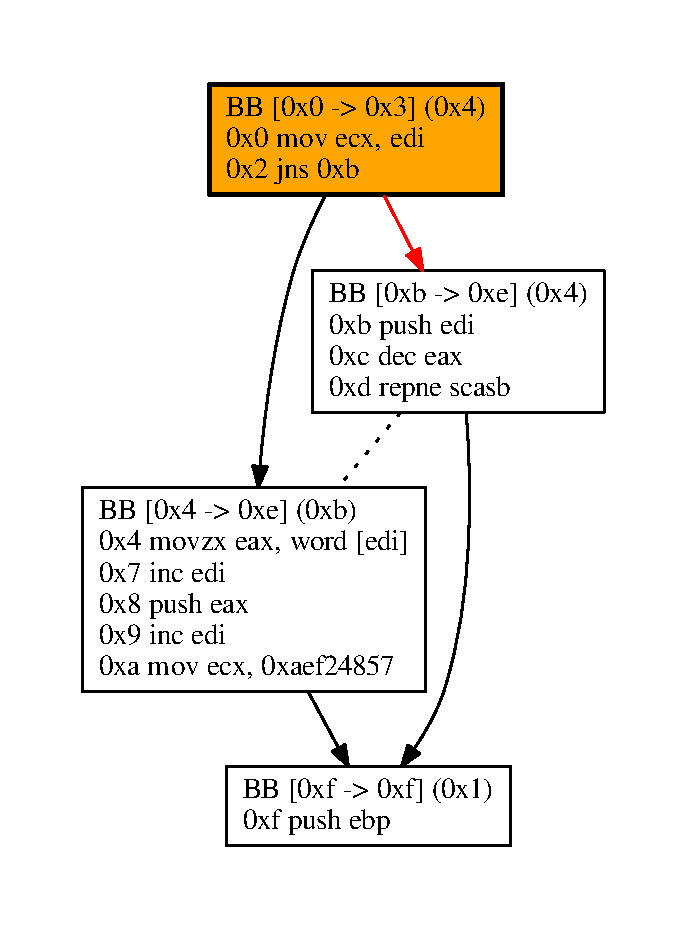
\includegraphics[width=0.4\textwidth]{supports/disasm/upx/upx.pdf}
\end{center}
\caption{Graphe de flot de contrôle de l'échantillon d'UPX}
\label{fig:upx_cfg}
\end{figure}

\FloatBarrier
\paragraph{Cacher une séquence de code de taille arbitraire.}
Jämthagen, Lantz et Hell \cite{JLH13} ont proposé un moyen d'inclure une longue séquence de code cachée au sein d'une séquence d'assembleur valide qui s'exécute sans provoquer d'erreur.

Une des possibilités est d'utiliser une instruction \nop\ avec préfixe qui se code sur neuf octets. La partie fixe (préfixe et opérande) est codée sur quatre octets (\texttt{66 0f 1f 84}) tandis que les cinq autres octets peuvent être choisis arbitrairement.
Ainsi chaque instruction \nop\ peut véhiculer 5 octets de code caché. Afin d'encoder une séquence de code dans une séquence de \nop\ il faut pouvoir utiliser les 4 octets fixes de l'instruction \nop\ suivante de manière utile ou non perturbante pour la séquence de code caché.
Une possibilité, si le registre \edx\ n'est pas utilisé dans la séquence à cacher, est de prendre \texttt{ba} pour dernier octet de chaque instruction \nop\ afin de former l'instruction \texttt{mov edx, 0x841f0f66} codée sur \texttt{ba 66 0f 1f 84}. On peut alors encoder n'importe quelles instructions de taille inférieure ou égale à quatre octets dans cette séquence de \nop.
Prenons la séquence d'octets suivante.
\begin{center}
\texttt{66 0f 1f 84} $\mathtt{x_1\ x_2\ x_3\ x_4}$ \texttt{ba 66 0f 1f 84} $\mathtt{y_1\ y_2\ y_3\ y_4}$ \texttt{ba 66 0f 1f 84} $\mathtt{z_1\ z_2\ z_3\ z_4}$.
\end{center}
Si on la désassemble linéairement à partir du premier octet il s'agit d'une séquence de trois \nop\ tandis que si on la désassemble à partir de $\mathtt{x_1}$, les instructions encodées dans les octets $\mathtt{x_i}$, $\mathtt{y_i}$ et $\mathtt{z_i}$ rentrent en considération :
\\

\begin{center}
\begin{tabular}{ll|ll}
\hline
 \multicolumn{2}{c|}{À partir du début} & \multicolumn{2}{c}{À partir de $x_1$} \\
\hline
 \texttt{66 0f 1f 84} $\mathtt{x_1\ x_2\ x_3\ x_4}$ \texttt{ba} & \nop & $\mathtt{x_1\ x_2\ x_3\ x_4}$ & ?\\
 \texttt{66 0f 1f 84} $\mathtt{y_1\ y_2\ y_3\ y_4}$ \texttt{ba} & \nop & \texttt{ba 66 0f 1f 84} & \texttt{mov edx, 0x841f0f66}\\
 \texttt{66 0f 1f 84} $\mathtt{z_1\ z_2\ z_3\ z_4}$ \texttt{ba} & \nop & $\mathtt{y_1\ y_2\ y_3\ y_4}$ & ?\\
  & & \texttt{ba 66 0f 1f 84} & \texttt{mov edx, 0x841f0f66}\\
    & & $\mathtt{z_1\ z_2\ z_3\ z_4}$ & ?\\
\end{tabular}
\end{center}

Les octets forment en fait deux chemins. L'un est exclusivement composé d'instructions \nop\ et est inoffensif : il s'agit du chemin d'exécution principal. Le second, le chemin d'exécution caché, débute à $\mathtt{x_1}$ et exécute le code que l'on souhaite dissimuler. En pratique le premier octet du chemin principal sera une cible valide et évidente du flot de contrôle tandis qu'il sera possible de sauter indirectement sur $\mathtt{x_1}$, par exemple avec un \texttt{jmp eax}. De cette manière le désassembleur est poussé à considérer le chemin principal sans examiner le chemin caché.

La limite est que les instructions cachées ne peuvent excéder une taille de 4 octets. Les auteurs expliquent cependant que beaucoup d'instructions \xq\ peuvent être séparées en plusieurs instructions plus petites, en utilisant par exemple des registres restreints comme \texttt{ax} ou \texttt{al} à la place d'\eax.

\section{Auto-modification}

% \begin{figure}
% \begin{center}
% \begin{tabular}{|l|l|l|}
% \hline
% Adresse & Octets & Instruction\\
% \hline
%  8048060  &  (...)         	& Pile -> RWX \\ 
%  804807c  &  bf 00 00 00 00         &  mov    edi, 0x0 \\
%  8048081  &  b8 91 80 04 08         &  mov    eax, 0x8048091 \\
%  8048086  &  66 c7 00 eb 00         &  mov    [eax], 0xeb \\
%  804808b  &  66 c7 40 01 07 00      &  mov    [eax+1], 0x7 \\
%  8048091  &  eb 0e                  &  jmp    80480a1 <edi3> \\
%  8048093  &  bf 01 00 00 00         &  mov    edi,0x1 \\
%  8048098  &  eb 0e                  &  jmp    80480a8 <fin> \\
%  804809a  &  bf 02 00 00 00         &  mov    edi,0x2 \\
%  804809f  &  eb 07                  &  jmp    80480a8 <fin> \\
%  80480a1  &  bf 03 00 00 00         &  mov    edi,0x3 \\
%  80480a6  &  eb 00                  &  jmp    80480a8 <fin> \\
%  80480a8  &  (...)		    &  Affiche edi \\
%  80480c3  &  (...)		    & Quitte \\
% \hline
% \end{tabular}
% \end{center}
% \caption{Exemple de code auto-modifiant}
% \label{fig:unevague_v0_code}
% \end{figure}

% \begin{figure}
% \begin{center}
% \subfigure[Code assembleur]{
% \begin{tabular}[b]{|l|l|l|}
% \hline
% Adresse & Octets & Instruction\\ 
% \hline
%  8048060  &  (...)         	& Pile -> RWX \\ 
%  804807c  &  bf 00 00 00 00         &  mov    edi, 0x0 \\
%  8048081  &  b8 91 80 04 08         &  mov    eax, 0x8048091 \\
%  8048086  &  66 c7 00 eb 00         &  mov    [eax], 0xeb \\
%  804808b  &  66 c7 40 01 07 00      &  mov    [eax+1], 0x7 \\
%  8048091  &  eb 0e                  &  jmp    80480a1 <edi3> \\
%  8048093  &  bf 01 00 00 00         &  mov    edi,0x1 \\
%  8048098  &  eb 0e                  &  jmp    80480a8 <fin> \\
%  804809a  &  bf 02 00 00 00         &  mov    edi,0x2 \\
%  804809f  &  eb 07                  &  jmp    80480a8 <fin> \\
%  80480a1  &  bf 03 00 00 00         &  mov    edi,0x3 \\
%  80480a6  &  eb 00                  &  jmp    80480a8 <fin> \\
%  80480a8  &  (...)		    &  Affiche edi \\
%  80480c3  &  (...)		    & Quitte \\
% \hline
% \end{tabular}
% \label{fig:unevague_v0_code}
% }
% \subfigure[Graphe de flot de contrôle]{
% 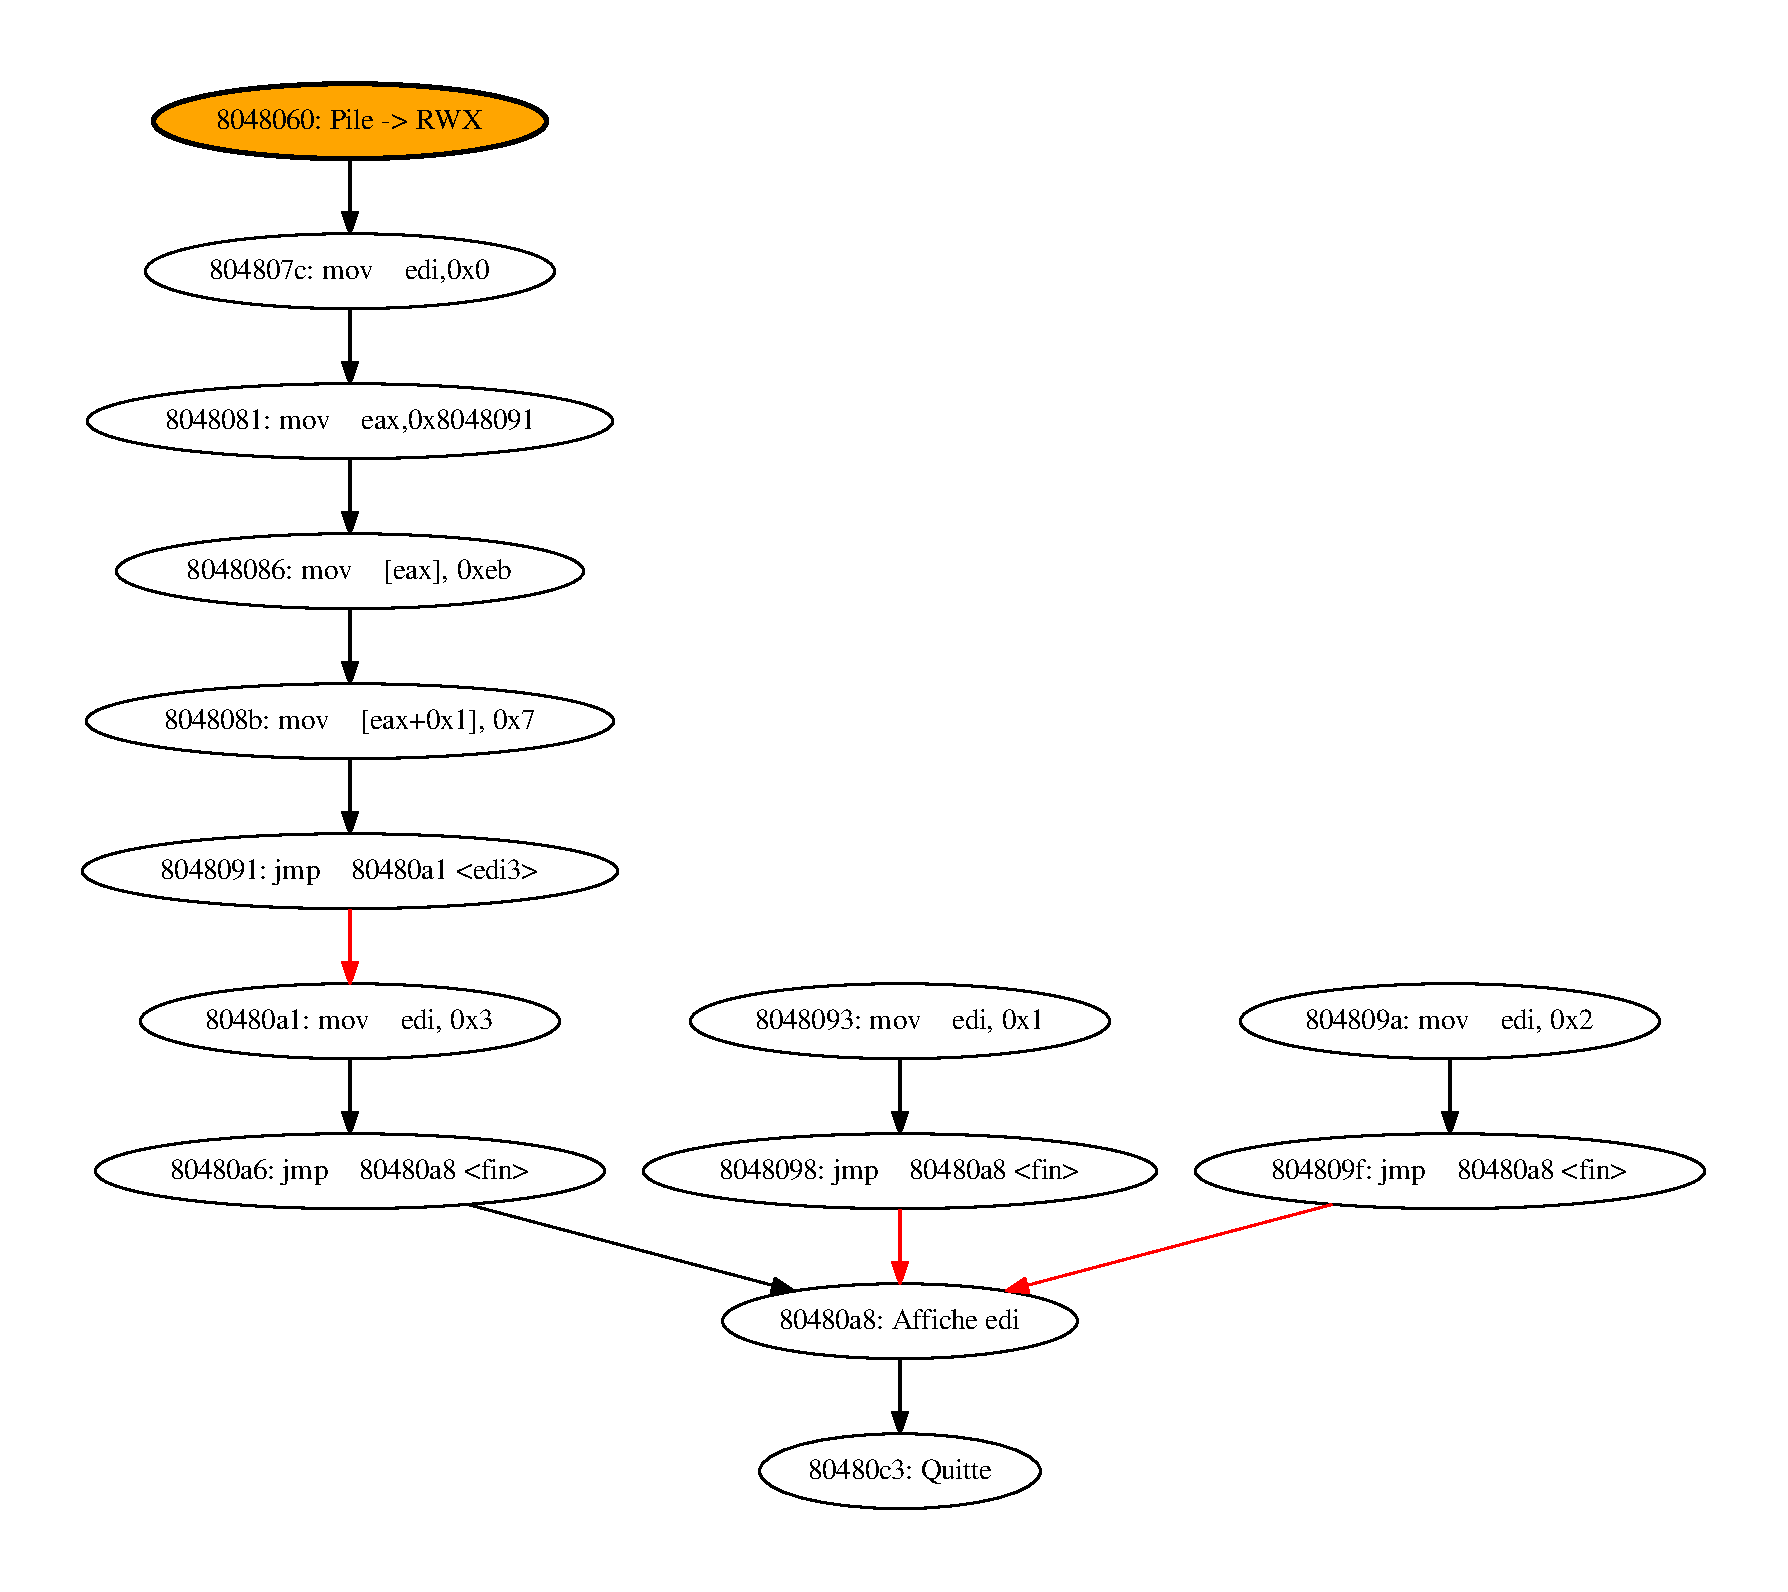
\includegraphics[width=1.0\textwidth]{supports/unevague/uv.pdf}
% \label{fig:unevague_v0_cfg}
% }
% \end{center}
% \ijym{détailler les ... (en annexe?)}
% \ijym{fonction f, adresses f, f+1, f+3, ...}
% \caption{Code assembleur auto-modifiant}
% \label{fig:unevague_v0}
% \end{figure}

Il a été expliqué dans la section \ref{section:assembleur} que, avec l'architecture de Von Neumann, le code n'est pas physiquement séparé des données lors de l'exécution sur une machine réelle.
Un programme auto-modifiant est simplement un programme utilisant cette propriété pour modifier le code assembleur le définissant au cours même de son exécution.
Ainsi on parle de comportement auto-modifiant lorsqu'une instruction du programme est codée sur au moins un octet qui a au préalable été modifié par ce programme.

En pratique les processeurs récents implémentent une protection, appelée bit NX ou W\textasciicircum X (prononcé ``W xor X''), permettant d'empêcher qu'une page mémoire puisse être à la fois écrite et exécutée lors de l'exécution du programme.
Cette protection a été ajoutée pour éviter des attaques par injection de code.
Ce type d'attaques résulte en l'exécution de code au sein de données entrées par l'utilisateur du programme.
Le choix d'activer ou non la protection revient au système d'exploitation mais en général ceux-ci l'autorisent par défaut parce que l'auto-modification a des cas d'utilisation légitimes.
De ce fait l'activation ou non de la protection est spécifiée lors de la compilation et si un programme n'est pas protégé il lui suffit d'utiliser un appel système (\texttt{mprotect} sous Linux) pour autoriser l'exécution de code dans les sections de données ou l'écriture dans les sections de code.

% Prenons le programme de la figure \ref{fig:unevague_v0_code}. Ce programme commence par autoriser l'accès en écriture à la section de code \ptext\ puis écrit sur la pile, modifie la valeur du registre \edi\ et termine par l'affichage de la valeur de \edi.
% Si on ne prend pas en compte l'écriture sur la pile, il semble évident au vu du graphe de flot de contrôle (Figure \ref{fig:unevague_v0_cfg}), vu que la première instruction de saut provoque un saut vers l'instruction \texttt{mov edi,0x3} et que la seconde provoque l'affichage de \edi, que la valeur finale du registre est 3.
% Pourtant les instructions \texttt{mov [eax],0xeb} et \texttt{mov [eax+1],0x07} aux l'adresse $0x8048086$ et $0x804808b$ remplacent le saut initial par un saut vers l'adresse $0x8048098$ où la valeur de \edi\ sera fixée à 2 avant l'affichage de celle-ci.

Prenons le programme de la figure \ref{fig:easy_sm}. Ce programme commence par autoriser l'accès en écriture à la section de code \ptext\ : les droits d'accès de cette section deviennent RWX (lecture, écriture et exécution sont autorisées).
Puis il place une adresse mémoire, \adr{8048076} dans \eax, puis l'instruction 2 écrit à l'adresse $eax+1$, provoquant la modification de l'instruction 4 en \texttt{mov edi, 2}, codée sur \texttt{bf 02 00 00 00}.
Puis l'instruction 3 provoque une seconde auto-modification en transformant l'instruction 5 en \texttt{mov ebx, 2}, codée sur \texttt{bb 02 00 00 00}.
Si on ne prend pas en compte les instructions auto-modifiantes la valeur finale, affichée, de \edi\ et \ebx\ est 1.
Pourtant les instructions 2 et 3 modifient le code de telle sorte que la valeur finale de ces deux registres soit 2 au moment de leur affichage.

\begin{figure}[h]
\begin{center}
\begin{tabular}[b]{|l|l|l|l|}
\hline
i & Adresse & Octets & Instruction\\ 
\hline
0 &  (...)   &  (...)                  &  \ptext\ -> RWX \\ 
1 & 8048060  &  b8 6b 80 04 08         &  mov    eax, 0x8048076\\
2 & 8048065  &  66 c7 40 01 02 00      &  mov    [eax+1], 2 \\
3 & 804806b  &  66 c7 40 06 02 00      &  mov    [eax+6], 2 \\
4 & 8048076  &  bf 01 00 00 00         &  mov    edi, 1 \\
5 & 804807b  &  bb 01 00 00 00         &  mov    ebx, 1 \\
6 &  (...)   &  (...)		       &  Affiche edi et ebx \\
7 &  (...)   &  (...)		       &  Quitte \\
\hline
\end{tabular}
\end{center}
\caption{Programme auto-modifiant}
\label{fig:easy_sm}
\end{figure}

On constate ici que le programme se modifie au cours de son exécution et donc on ne peut pas se contenter de la représentation d'origine du programme pour l'analyser.
De plus les instructions modifiées pourraient modifier le flot de contrôle du programme en rajoutant des instructions de saut conditionnel par exemple, donc le graphe de flot de contrôle initial peut être amené à évoluer au cours de l'exécution du programme.


\section{Logiciels malveillants et obscurcissement}
Un programmeur cherchant à protéger son binaire va se tourner vers les techniques d'obscurcissement dont nous avons donné quelques exemples ci-dessus. Puisque chacune des transformations a pour effet de rendre le programme plus difficile à comprendre, il n'y a souvent pas de limite au nombre de fois qu'il est possible d'itérer une technique de protection particulière. On peut alors chercher un compromis entre niveau de protection et complexité ajoutée au programme (en temps, en taille et en mémoire utilisée).

En pratique les auteurs des logiciels malveillants utilisent des logiciels existants pour protéger leurs binaires.
Ces logiciels de protection s'appliquent à l'ensemble du programme malveillant sans avoir à définir des atouts particuliers à protéger. On appelle ces programmes des empaqueteurs (\emph{packers}) : un empaqueteur prend un binaire en entrée et produit en sortie un binaire empaqueté, protégé. Une technique couramment utilisée est de cacher le binaire d'origine dans les données du binaire empaqueté, par exemple chiffré ou compressé (voir figure \ref{fig:packer}). Lors de l'exécution du binaire protégé une première phase consiste à restaurer le binaire d'origine en mémoire puis à effectuer un saut vers le point d'entrée du code restauré, provoquant ainsi l'exécution du binaire d'origine.

\begin{figure}[h]
\begin{center}
\scalebox{1}{
\begin{tikzpicture}[->,scale=1,>=stealth',thick]
\node[state, text width=3cm, minimum size=3cm] (BIN){Binaire d'origine};
\node[state, below right = -0.5cm and 4cm of BIN.east, text width=3cm, minimum size=3cm] (BINO){Données :\\Binaire d'origine caché};
\node[state, below = -2cm of BINO.north, text width=3cm, minimum size=2cm] (UNPACK){Code :\\Routine de dépaquetage};
% \draw ($(BIN.north west) + (-0.8, -0.1) $) -- node[left=0.3cm]{Point d'entrée} ($(BIN.north west) + (0, -0.1) $);
% \draw ($(UNPACK.north east) + (0.8, -0.1) $) -- node[right=0.3cm]{Point d'entrée} ($(UNPACK.north east) + (0, -0.1) $);
\draw ($(BIN.east) + (0.5, 0) $) -- node[below]{\large Enpaquetage} ($(BIN.east) + (3cm, 0) $);
\node [fit={($(UNPACK.north west) + (-0.1, 0.1)$) ($(BINO.south east) + (0.1, -0.1)$)}, draw, label=Binaire empaqueté] {};
\end{tikzpicture}
}
\end{center}
\caption{Empaquetage d'un binaire}
\label{fig:packer}
\end{figure}

L'empaqueteur libre UPX \cite{UPX} est un cas typique du schéma précédent. Il compresse le binaire d'origine et le restaure à l'exécution. Ainsi il est plutôt conçu pour optimiser la taille du binaire paqueté et non pour l'obscurcir. La transformation utilisée étant réversible, l'empaqueteur permet également de récupérer le programme binaire d'origine sans l'exécuter. Il est cela dit parfois utilisé par des auteurs de logiciels malveillants sous une forme modifiée ne permettant plus de le dépaqueter automatiquement.


\section{Conclusion}
Cette thèse s'intéresse particulièrement à l'analyse des programmes écrits en assembleur \xq\ et \xs. Ces programmes ont en général été compilés à partir d'un langage de haut niveau puis ont été modifiés à l'aide d'un logiciel de protection. Les binaires que l'on étudie sont donc protégés avec des techniques statiques et l'emploi de l'auto-modification. Notre travail consiste alors à chercher à désassembler correctement ces programmes dans le but de faciliter leur analyse.

Les chapitres suivants détailleront plusieurs techniques d'analyse que nous avons appliquées. 
Dans un premier temps nous nous intéresserons à l'aspect auto-modifiant des programmes et verrons comment l'analyse dynamique peut être utilisée pour reconstruire un modèle pour le programme auto-modifiant. 
Nous introduirons ensuite des techniques d'analyse statiques pour chercher à construire un graphe de flot de contrôle approximant le graphe de flot de contrôle parfait et contourner certaines méthodes de protection comme le chevauchement de code.


\DontFrameThisInToc
\chapter{Analyse statique et chevauchement de code\label{chap:chevauchement}}
Nous cherchons à parcourir le plus de code atteignable dans le but d'approximer le graphe de flot de contrôle parfait.
Il faut alors pallier à l'incomplétude d'un parcours récursif et au manque de précision d'un parcours linéaire.
Une des difficulté vient de l'obscurcissement par chevauchement de code. 
Dans ce chapitre nous commençons par dresser un état de l'art de quelques techniques d'analyse statique et de leur approche du chevauchement de code, puis nous proposerons une caractérisation des binaires utilisant cette technique.
% Nous cherchons donc des approches du désassemblage qui prennent en compte cette méthode de protection.


\section{Revue de littérature}
% \subsection{Couverture de code}
Bien que le problème du chevauchement de code ne soit pas une technique d'obscurcissement récente et soit bien documenté \cite{PMA}, la littérature portant sur le désassemblage fait souvent l'hypothèse qu'un octet à une adresse spécifique ne peut être présent que dans une seule instruction \cite{KruegelRVV04}. 
Cette contrainte empêche de détecter tout chevauchement mais permet un désassemblage plus précis sur un binaire qui n'utilise pas cette technique de protection.


\paragraph{Parcours spéculatif.}
Le parcours récursif étant moins sensible à des obscurcissements très simples comme l'injection de code mort, il est souvent pris comme point de départ dans les recherches sur le désassemblage statique.
Une fois une première recherche de code avec un parcours récursif effectuée, les octets restants peuvent subir un parcours linéaire qui cherchera à déterminer s'ils sont du code ou des données à l'aide d'heuristiques.
Une de ces approche évalue la probabilité qu'une suite d'octets soit effectivement du code en apprenant au préalable des suites d'octets codant réellement des instructions lancées lors de l'exécution de programmes \cite{KDF09}.
On appelle cet enchaînement des deux parcours un parcours spéculatif.

Prasaf et Chiueh \cite{PC03}, après un premier désassemblage récursif, tentent d'identifier les adresses de début de fonctions assembleur à l'aide de la suite d'instruction \push\ puis \mov, caractéristique de fonctions compilées : elles commencent par empiler le pointeur de pile de base avec \texttt{push ebp} pour le remplacer par le pointeur de pile avec \texttt{mov ebp, esp}. Ils identifient également toutes les adresses où sont codées une instruction valide. À partir de ces adresses ils effectuent à nouveau un parcours récursif jusqu'à une instruction de saut inconditionnel (\ret\ out \jmp), estimant que la séquence de code identifiée s'arrête sur ce saut. Le risque est grand que des chemins parcourus ainsi ne soient pas valides, ils éliminent alors les chemins qui aboutissent sur du code invalide ou des adresses connues pour être des données.

Krügel, Roberston, Valeur et Vigna \cite{KruegelRVV04} proposent aussi de séparer le code en fonctions assembleur. Ils effectuent une première analyse récursive pour détecter le maximum d'instructions atteignables et, lorsque que deux ou plusieurs instructions atteignables se chevauchent, ils considèrent qu'il s'agit d'un conflit qui se résoudra par le choix d'une des instructions.
Leurs hypothèses sont : (i) les instructions ne peuvent pas se chevaucher, (ii) les sauts conditionnels peuvent être suivis ou non, (iii) le binaire peut contenir du code mort, et (iv) le code suivant une instruction \call\ n'est pas nécessairement accessible. Pour résoudre les conflits de chevauchement ils favorisent les instructions atteignables depuis le point d'entrée (que l'on sait accessible), puis ils considèrent qu'une instruction permettant d'atteindre directement deux instructions qui se chevauchent n'est pas valide et enfin ils favorisent les instructions les plus connectées au graphe de flot de contrôle.
Leur approche est un point de départ pour le désassemblage de binaires obscurcis. Ils prennent par exemple en compte l'ajout de code mort et certaines modifications du flot de contrôle.

Schwarz, Debray et Andrews \cite{SDA02} introduisent un parcours linéaire capable de détecter certaines injections de données dans le code, comme les tables de saut (souvent présent dans du code compilé en C ou C++). Ils proposent de combiner les parcours récursifs et linéaires pour détecter les anomalies dans le désassemblage. Si, au sein d'une fonction, une instruction provenant du désassemblage récursif chevauche une instruction provenant du désassemblage linéaire, le désassemblage de la fonction est considéré comme contenant une erreur.
% \\

Partant du principe qu'un désassemblage correct ne contient pas de chevauchement de code, ces approches ne sont pas satisfaisantes pour désassembler des binaires utilisant du chevauchement de code, tels les programmes protégés avec \telock.
% \\


\paragraph{Désassembleurs disponibles.}
Les désassembleurs existants, qu'ils utilisent un parcours linéaire ou récursif, font l'hypothèse que le code ne peut pas se chevaucher et ne parviennent pas à afficher un désassemblage cohérent dans le cas contraire.

Le désassemblage récursif de l'exemple de \telock\ (figure \ref{fig:telock_obf_disas}) avec IDA Pro (version 6.3) \cite{IDA} est le suivant :
\begin{lstlisting}[language={[x86masm]Assembler}, escapechar=~]
01006E7A     inc     byte ptr [ebx+ecx]
01006E7D     jmp     short near ptr loc_1006E7D+1
; ~Les octets qui suivent n'ont pas été désassemblés~
01006E7F     db 0C9h
01006E80     db  7Fh
01006E81     db 0E6h
01006E82     db  8Bh
01006E83     db 0C1h
\end{lstlisting}
Radare \cite{radare} effectue le désassemblage linéaire suivant :
\begin{lstlisting}[language={[x86masm]Assembler}, escapechar=~]
01006e7a    fe 04 0b     inc byte [ebx+ecx]
01006e7d    eb ff        jmp 6e7e
01006e7f    c9           leave
01006e80    7f e6        jg 6e68
01006e82    8b c1        mov eax, ecx
\end{lstlisting}
Ni l'un ni l'autre n'est capable de suivre le saut de l'instruction \jmp\ : la cible du saut a déjà été prise en compte comme faisant partie d'une autre instruction.

De même ni Radare ni IDA ne détectent le second chemin d'exécution dans l'extrait d'UPX (figure \ref{fig:upx_obf_disas}) et désassemblent cet extrait comme suit.
\begin{lstlisting}[language={[x86masm]Assembler}, escapechar=~]
010059f0    89 f9            mov ecx, edi
010059f2    79 07            jns 0x10059fb
010059f4    0f b7 07         movzx eax, word [edi]
010059f7    47               inc edi
010059f8    50               push eax
010059f9    47               inc edi
010059fa    b9 57 48 f2 ae   mov ecx, 0xaef24857
010059ff    55               push ebp
\end{lstlisting}

\paragraph{Approches prenant en compte le chevauchement.}
Les auteurs de la technique de chevauchement détaillée au chapitre \ref{chap:obscurcissement}, permettant d'encoder une séquence de code cachée dans une séquence \cite{JLH13}, proposent de détecter la protection qu'ils exposent. 
L'idée est qu'il est improbable qu'une longue séquence d'octets représente une séquence valide de code. 
Si une telle séquence existe, c'est sûrement du code. Ainsi si deux longues séquences valides de code se chevauchent, il s'agit d'un obscurcissement délibéré et une des deux séquences contient du code caché. 
Cette approche fonctionne pour la protection qu'ils exposent mais n'est pas applicable aux cas d'UPX par exemple car les séquences d'octets sur lesquels des instructions se chevauchent sont très courtes et il est plausible que le chevauchement soit accidentel et que le code en chevauchement ne soit pas atteignable.

Dans sa thèse, Kinder \cite{Kinder10} indique que si la technique de désassemblage autorise que différentes instructions dans le graphe de flot de contrôle se chevauchent et réalise des désassemblages atomiques d'une seule instruction à la fois à partir de chaque adresse, alors on peut voir deux instructions qui se chevauchent comme indépendantes.

Effectivement les travaux présentés dans cet état de l'art ainsi que les désassembleurs existants prennent pour hypothèse que le code ne doit pas se chevaucher alors que nous avons représenté les chevauchements de \telock\ et UPX très simplement. 
L'hypothèse d'alignement permet en général de simplifier les critères de désassemblage et est justifiée par la non occurrence de ce phénomène dans des programmes légitimes.
Nous verrons qu'en pratique l'utilisation du chevauchement de code est rare même dans un binaire protégé et nous proposerons une technique de désassemblage capable de détecter les cas de chevauchement.

\section{Analyse statique du chevauchement de code}
Nous proposons une formalisation du problème du chevauchement de code.
Du point de vue du désassemblage, un programme qui présente une unique instruction qui en chevauche une autre peut se voir comme composé d'un chemin principal de désassemblage et d'un chemin secondaire dans lequel l'instruction en chevauchement se place.
Reprenons l'exemple de \telock : le segment d'octets \texttt{eb ff c9 7f e6} peut se voir comme composé des deux \layers\ de code données à la figure \ref{fig:telock-layers-simple} : il y a deux \layers, la première contient les instructions \texttt{jmp +1}, \texttt{leave} et \texttt{jg 0x1006e68} et la seconde contient l'instruction \texttt{dec ecx}, chevauchant \texttt{jmp +1}.
En fait le segment d'octets \texttt{eb ff c9 7f e6} contient exactement les quatre instructions précédentes : il y a au maximum une instruction valide à chaque adresse et la dernière instruction potentielle, codée sur \texttt{e6}, n'est pas valide.


\begin{figure}[h]
\begin{center}
\begin{tabular}{|l|c|c|c|c|c|}
\hline
Adresses & 0x01006e7d & 0x01006e7e & 0x01006e7f & 0x01006e80 & 0x01006e81\\
\hline
Octets & eb & ff & c9 & 7f & e6\\
\hline
\Layer\ 1 & \multicolumn{2}{c|}{jmp +1} & leave & \multicolumn{2}{c|}{jg 0x1006e68}\\
\hline
\Layer\ 2 & \cnoir & \multicolumn{2}{c|}{dec ecx} & \multicolumn{2}{c|}{\cnoir} \\
 \hline
% \\
\end{tabular}
\end{center}
\caption{Découpage cohérent en \layers\ de l'extrait de \telock}
\label{fig:telock-layers-simple}
\end{figure}

% \begin{figure}
% \begin{center}
% \begin{tabular}{|l|c|c|c|c|c|}
% \hline
% Adresses & 0x01006e7d & 0x01006e7e & 0x01006e7f & 0x01006e80 & 0x01006e81\\
% \hline
% Octets & eb & ff & c9 & 7f & e6\\
% \hline
% \Layer\ 1 & \multicolumn{2}{c|}{jmp +1} & \cnoir & \multicolumn{2}{c|}{jg 0x1006e68}\\
% \hline
% \Layer\ 2 & \cnoir & \multicolumn{2}{c|}{dec ecx} & \multicolumn{2}{c|}{\cnoir} \\
%  \hline
% % \\
% \end{tabular}
% \end{center}
% \caption{\Layers\ de l'extrait de \telock}
% \label{fig:telock-layers-recursive}
% \end{figure}

Formellement on définit une \layer\ comme un ensemble d'instructions qui ne se chevauchent pas (définition \ref{def:layer}).
Par conséquent lors du désassemblage on cherche à effectuer un découpage cohérent des instructions inclues dans le graphe de flot de contrôle en différentes \layers. Un découpage cohérent est simplement la donnée d'un ensemble de \layers\ deux à deux disjointes et recouvrant l'ensemble des instructions désassemblées.
L'exemple précédent pour \telock\ est un découpage cohérent.

\begin{defi}
 Une \layer\ de code $L$ est un ensemble d'instructions dynamiques qui ne se chevauchent pas : $\forall D_1, D_2\in L,\ $\dc{D_1}$\cap$\dc{D_2}$=\emptyset$ où \dc{D} est l'intervalle des adresses sur lesquelles D est codée.
\label{def:layer}
\end{defi}

\paragraph{Borne du nombre de \layers.}
Le nombre minimal de \layers\ permettant de former un découpage cohérent est borné par la taille maximale des instructions, c'est à dire 15 octets pour l'assembleur \xq.
Pour s'en convaincre il suffit de définir le découpage cohérent suivant. Pour un segment d'octets à l'adresse \adr{a}, on place dans la \layer\ i, pour $1\leq i\leq 15$ toutes les instructions aux adresses congrues à $a+i-1 (mod\ 15)$. C'est à dire que la \layer\ 1 contient les instructions aux adresses \adr{a}, \adr{a+15}, \adr{a+30}, etc ; la \layer\ 2 celles aux adresses \adr{a+1}, \adr{a+16}, \adr{a+31}, etc. Puisque les instructions dans chaque \layer\ sont distantes de 15 octets, il ne peut pas y avoir de chevauchement au sein d'une \layer\ et les \layers\ sont disjointes ; il s'agit bien d'un découpage cohérent une fois qu'on enlève les \layers\ ne contenant pas d'instructions valides. Ce découpage contient au plus 15 \layers.
\itodo{l'exemple qui donne 15 layers ?}

Nous définirons par la suite plusieurs découpages cohérents en \layers\ et discuterons de leur pertinence et de leurs implémentations.


\subsection{\Layers\ linéaires}
Une approche naturelle des \layers\ consiste à construire une première \layer\ par parcours linéaire à partir du début de la section de code du binaire.
Cette première \layer\ contient exactement les instructions qu'un désassembleur par parcours linéaire aurait détecté.
Les \layers\ suivantes seront construites également par parcours linéaire, à partir de chaque adresse du binaire.
Ainsi on peut construire une \layer\ de code à partir de chaque adresse du binaire.
Un tel découpage pour \telock\ donne les layers indiqués en figure \ref{fig:telock-layers-linear}.

Ce découpage est donc, par définition, basé sur l'alignement des instructions : au sein d'une \layer, les instructions sont alignées, c'est à dire qu'un désassemblage linéaire depuis la première instruction de la \layer\ parcourt toutes les autres instructions de la \layer. 
Il est à noter qu'en assembleur \xq\ ou \xs\ les instructions ont tendance à se réaligner rapidement : si deux instructions se chevauchent et qu'on l'on réalise un parcours linéaire depuis chacune d'entre elles, il suffit en général d'au plus quatre \todo{cite, vrai?}instructions pour que ces deux parcours se confondent.
Cette propriété a pour conséquence que la plupart des \layers\ linéaires se réalignent sur une \layer\ précédente, en général la première. Sur la figure \ref{fig:telock-layers-linear} les \layers\ 1 et 2 se réalignent et partagent l'instruction \texttt{jg 0x1006e68}.
Cette propriété n'est évidemment pas vérifiée si les instructions ont été spécialement choisie pour provoquer de longs chemins de chevauchement, comme avec l'obscurcissement précédemment cité \cite{JLH13}.

Nous souhaitons obtenir un découpage cohérent des \layers\ sous forme d'ensembles deux à deux disjoints.
Il suffit alors d'enlever des \layers\ les instructions existant déjà dans les \layers\ inférieures (colorées en gris sur la figure \ref{fig:telock-layers-linear}) et de ne garder que les \layers\ contenant des instructions valides.
Au final il reste les deux \layers\ données précédemment à la figure \ref{fig:telock-layers-simple}, obtenus linéairement.

\paragraph{Binaire composé de plusieurs segments.}
On peut étendre la définition précédente applicable à un segment d'octets à un binaire composé de plusieurs segments de code disjoints.
L'extension consiste à simplement à réaliser un découpage cohérent pour chaque segment puis à les réunir au sein d'un seul découpage par une union des \layers\ qui les composent, lui aussi cohérent puisque les segments sont deux à deux disjoints.

\paragraph{\Layers\ linéaires et désassemblage.}
% Les \layers\ linéaires sont en fait une extension du désassemblage linéaire. Un programme non obscurcis peut être désassemblé avec un minimum d'erreurs par un parcours linéaire représenté.
Le découpage en \layers\ linéaires n'est pas en soi un algorithme de désassemblage : il s'agit d'une analyse exhaustive de toutes les instructions codées dans le segment analysé, elle est donc par définition incorrecte.
On peut voir ce découpage comme une caractéristique du binaire qui contient l'ensemble des instructions potentiellement exécutées (hors auto-modification) et qui dépend de leur agencement en mémoire.


\paragraph{Caractérisations des binaires obscurcis.}
Considérons un programme désassemblé en son graphe de flot de contrôle parfait.
Si chaque instruction du graphe de flot de contrôle, présente dans le segment $s$, fait partie de la première \layer\ du découpage linéaire de $s$, il est clair qu'il n'y a pas de chevauchement de code possible.
En pratique c'est le cas la plupart du temps avec des binaires non obscurcis\todo{vrai?}.
L'inverse n'est par contre pas vrai puisque deux instructions peuvent ne pas être alignées à cause d'un ajout de code mort (voir chapitre \ref{chap:obscurcissement}) sans qu'il n'y ait de chevauchement de code dans le graphe de flot.

Lors du désassemblage d'un binaire plusieurs métriques peuvent être observées.
On peut d'une part observer combien de \layers\ différentes sont utilisées : chaque \layer, en dehors de la première de chaque segment, atteste du départ d'un chemin désaligné avec le chemin principal.
D'autre part on peut compter le nombre de sauts d'une instruction d'une \layer\ vers une instruction désalignée d'une autre \layer. Dans le cas de \telock, le saut depuis l'instruction \texttt{dec ecx} à l'adresse \adr{0x01006e7e} vers l'instruction \texttt{jg 0x1006e68} à l'adresse \adr{0x01006e80}, bien qu'il provoque un changement de \layer, n'est pas désaligné. Le nombre de ces sauts de désalignement atteste de la prévalence des chemins représentés par chaque \layer.

\itodo{rapport à un désassemblage linéaire}

\begin{figure}
\begin{center}
\begin{tabular}{|l|c|c|c|c|c|}
\hline
Adresses & 0x01006e7d & 0x01006e7e & 0x01006e7f & 0x01006e80 & 0x01006e81\\
\hline
Octets & eb & ff & c9 & 7f & e6\\
\hline
\Layer\ 1 @0x01006e7d & \multicolumn{2}{c|}{jmp +1} & leave & \multicolumn{2}{|c|}{jg 0x1006e68}\\
\hline
\Layer\ 2 @0x01006e7e & \cnoir & \multicolumn{2}{c|}{dec ecx} & \multicolumn{2}{|c|}{jg 0x1006e68 \cgris} \\
\hline
\Layer\ 3 @0x01006e7f & \multicolumn{2}{c|}{\cnoir} & leave \cgris & \multicolumn{2}{|c|}{jg 0x1006e68 \cgris} \\
\hline
\Layer\ 4 @0x01006e80 & \multicolumn{3}{c|}{\cnoir} & \multicolumn{2}{|c|}{jg 0x1006e68 \cgris} \\
\hline
\Layer\ 5 @0x01006e81 & \multicolumn{4}{|c|}{\cnoir} & (invalide) \\
\hline
% \\
\end{tabular}
\end{center}
\caption{\Layers\ linéaires de l'extrait de \telock}
\label{fig:telock-layers-linear}
\end{figure}

% \begin{figure}
% \begin{center}
% \begin{tabular}{|l|c|c|c|c|c|c|c|c|c|c|}
% \hline
% Addresses & 0xf2 & 0xf3 & ... & 0xf9 & 0xfa & 0xfb & 0xfc & 0xfd & 0xfe & 0xff\\
% \hline
% Bytes & 79 & 07 & ... & 47 & b9 & 57 & 48 & f2 & ae & 55\\
% \hline
% Layer 1 @0xf2 & \multicolumn{2}{c|}{jns +9 (0xfb)} & ... & inc edi & \multicolumn{5}{c|}{mov ecx, aef24857} & push ebp\\
% \hline
% Layer 2 @0xfb & \multicolumn{5}{c|}{\cnoir} & push edi & dec eax & \multicolumn{2}{c|}{repne scasb} & push ebp\\
% \hline
% % \\
% \end{tabular}
% \end{center}
% \caption{Layers of a subset of the UPX code segchevment}
% \label{fig:upx-layers-recursive}
% \end{figure}

\subsection{\Layers\ désassemblées}
Une autre approche consiste à construire des \layers\ de code au fur et à mesure du désassemblage du binaire.
Un désassemblage parfait de l'extrait de \telock\ précédent (figure \ref{fig:telock-layers-simple}) à partir du point d'entrée \adr{0x1006e7d} contient exactement les trois instructions \texttt{jmp +1}, \texttt{dec ecx}, \texttt{jg 0x1006e68}. La première instruction va provoquer la création d'une première \layer, la seconde étant en chevauchement avec la première, elle ne peut être placée que dans une nouvelle \layer. La dernière instruction peut être placée dans n'importe laquelle des deux \layers\ existantes, on la placera, arbitrairement, dans la première \layer. Un tel découpage est donné en figure \ref{fig:telock-layers-rec}.

\begin{figure}[h]
\begin{center}
\begin{tabular}{|l|c|c|c|c|c|}
\hline
Adresses & 0x01006e7d & 0x01006e7e & 0x01006e7f & 0x01006e80 & 0x01006e81\\
\hline
Octets & eb & ff & c9 & 7f & e6\\
\hline
\Layer\ 1 & \multicolumn{2}{c|}{jmp +1} & \cnoir & \multicolumn{2}{c|}{jg 0x1006e68}\\
\hline
\Layer\ 2 & \cnoir & \multicolumn{2}{c|}{dec ecx} & \multicolumn{2}{c|}{\cnoir} \\
 \hline
% \\
\end{tabular}
\end{center}
\caption{Découpage cohérent en \layers\ lors du désassemblage récursif de \telock}
\label{fig:telock-layers-rec}
\end{figure}

% Nous allons définir un algorithme de découpage cohérent en \layers\ lors d'un désassemblage récursif qui sera repris dans notre proposition de désassembleur. Nous tenterons \todo{ahah} de prouver quelques propriétés sur le découpage qui en résulte.

L'algorithme \ref{algo:ajout_inst_layers} explicite le choix fait lors de l'insertion d'une instruction dans un découpage cohérent existant : on choisit simplement la première \layer\ dont les instructions ne chevauchent pas l'instruction à ajouter. La création d'une nouvelle \layer\ peut être nécessaire. Ce découpage étant minimal [à prouver] \todo{à prouver}, il ne peut pas dépasser 15 \layers.

\begin{algorithm}[H] %or another one check
\caption{Ajout d'une instruction à un découpage cohérent en \layers}
\SetAlgoLined
\KwIn{Un découpage cohérent $C$ en $n$ \layers\ $L_i$, une instruction $D$}
\KwResult{Un découpage cohérent contenant l'instruction $D$}
\SetKwProg{Fn}{}{}{}
\SetKwFunction{FRecurs}{ajoutInstruction}
\Fn(
% \tcc*[h]{C : matrice des associations possibles, i : numéro du prochain sommet de P à associer, F : liste des couples d'associations déjà faites}
){\FRecurs{C, D}}{
\eIf {l'instruction D n'est pas comprise dans C} {
  \For {$i$ de $1$ à $n$}{
    \If {$\forall$ instruction $D'\in L_i$, D et D' ne se chevauchent pas}{
      $L_i\leftarrow L_i\cup \{D\}$\\
      \Return $C$
    }
  }
  $L_{n+1}\leftarrow\ \{D\}$ \\
  $C\leftarrow C\cup\{L_{n+1}\}$ \\
  \Return $C$
}
{
  \Return $C$
}
}
\label{algo:ajout_inst_layers}
\end{algorithm}

\paragraph{Non-unicité du découpage pour un parcours récursif.}
La technique de désassemblage que nous proposons est basée sur un parcours récursif. Il est à noter qu'avec ce type de parcours les \layers\ obtenus en applicant l'algorithme précédent dépendent de l'ordre dans lequel les fils de chaque sommet sont explorés.

Reprenons un graphe de flot simplifié de l'échantillon d'UPX donné au chapitre \ref{chap:obscurcissement}, donné en figure \ref{fig:upx_cfg_simple}. Le sommet 1 est le point d'entrée, le sommet 4 le point d'arrêt et les instructions aux sommets 2 et 3 se chevauchent. Le sommet 1 a deux fils : le sommet 2 qui est accessible séquentiellement (les instructions se suivent) et le sommet 3 qui est la cible d'un saut.

Le découpage sera composé de deux \layers\ dans tous les cas mais si l'on parcourt d'abord le sommet 2 alors les deux \layers\ sont $L_1=\{1, 2, 4\}$ et $L_2=\{3\}$. Au contraire si l'on choisit de d'abord parcourir le sommet 3, les \layers\ sont $L_1=\{1, 3, 4\}$ et $L_2=\{2\}$.

\begin{figure}
\begin{center}
\includegraphics[width=0.2\textwidth]{supports/disasm/upx/upx_simple.pdf}
\end{center}
\caption{Graphe de flot de contrôle simplifié de l'échantillon d'UPX}
\label{fig:upx_cfg_simple}
\end{figure}

\paragraph{Métriques.}
Le découpage précis en \layers\ dépend de la manière dont le parcours récursif est effectué mais \todo{à prouver} le nombre de \layers\ ainsi que le nombre de sauts de changement de \layers\ n'en dépendent pas.
On utilisera le nombre de \layers\ pour observer la complexité des chevauchements de code tandis que le nombre de sauts de changement de \layers\ indique la fréquence d'utilisation de cette technique d'obscurcissement.


\itodo{Découpage cohérent minimal.}
\itodo{discussion : pourquoi on préfère celui là ?}

\DontFrameThisInToc
\chapter{Sémantique de l'assembleur et langage intermédiaire\label{chap:semantique}}
% \section{Sémantique concrète pour un langage assembleur}

Dans ce chapitre nous proposons un modèle de langage simplifié pour l'assembleur et une sémantique concrète pour ce langage.

Lors de l'analyse d'un binaire, il est crucial de pouvoir analyser chaque instruction.
La question centrale est la suivante : quelle est l'opération réalisée par cette instruction ?
En particulier quels sont ses opérandes d'entrée, de sortie, et comment sont-ils lus et modifiés ?
Prenons l'instruction \texttt{push ecx}. 
Il est clair que le registre \ecx\ est un opérande mais cette information est insuffisante : cette instruction consiste à empiler la valeur de \ecx\ sur la pile, elle modifie donc le pointeur de pile \esp\ et écrit à une adresse mémoire.

Nous reprenons la classification informelle en trois niveaux d'information proposée par Calvet \cite{Calvet2013} à la figure \ref{fig:niveaux_sem}, par exemple pour l'instruction \texttt{push ecx} :
\begin{itemize}
 \item Niveau 1 - Opérandes explicites : \ecx
 \item Niveau 2 - Opérandes implicites précis : \ecx\ et \esp\ sont des entrées, l'adresse mémoire à l'adresse $esp-4$ est une sortie
 \item Niveau 3 - Opération : l'instruction décrémente \esp\ de 4 puis écrit à l'adresse mémoire pointée par \esp\ la valeur qui est dans \ecx
\end{itemize}

\begin{figure}
\begin{center}
\begin{tikzpicture}[text centered]
% Definition of circles
\colorlet{circle edge}{black!100}
\colorlet{circle area}{black!20}

\tikzset{filled/.style={fill=circle area, draw=circle edge, thick},
    outline/.style={draw=circle edge, thick}}
    \draw (0, -1) arc (-90:270:2.7cm) node[above=4.25cm, text width=4cm]{3\\Opération};
    \draw (0, -1) arc (-90:270:2.1cm) node[above=2.4cm, text width=4cm]{2\\Opérandes\\implicites};
    \draw (0, -1) arc (-90:270:1.2cm) node[above=0.4cm, text width=4cm]{1\\Opérandes\\explicites};
%     \node[anchor=south] at (current bounding box.north) {Progwramme};
\end{tikzpicture}
\end{center}
\caption{Niveaux de précision des informations sur une instruction}
\label{fig:niveaux_sem}
\end{figure}

Une sémantique concrète se place au niveau 3 : elle donne une information exhaustive sur l'opération réalisée par chaque instruction.
Ce chapitre sera donc consacré à la définition d'une sémantique concrète pour un langage assembleur simplifié.
Nous verrons par la suite que pour certaines analyses une sémantique de niveau 2 peut-être suffisante.

\section{Sémantique concrète pour un langage assembleur}
\paragraph{Représentation de la mémoire et des registres.}
On peut voir la mémoire comme un tableau indexé sur les entiers contenant la pile et le tas. Les registres sont des variables distinctes de la mémoire et sont en nombre limité.
L'assembleur distingue plusieurs modes d'adressage dont les adressage direct et indirect : à l'exécution \eax\ prend la valeur du registre \eax\ (adressage direct) tandis que \texttt{[eax]} fait référence à la valeur en mémoire à l'adresse contenue dans \eax\ (adressage indirect).
Ces éléments sont définis formellement à la définition \ref{def:sem_conc_var} : $\BA$ est l'ensemble des registres et $\BT$ représente la mémoire comme un tableau.

% \begin{rem}
%  Avec cette définition, une valeur en mémoire peut pointer vers un registre. De même un registre peut pointer vers un autre registre.
%  Ces deux possibilités ne sont pas réalisables avec l'assembleur \xq\ ou \xs.
% \end{rem}


% \begin{defi}
% On définit les symboles $x\in\BX$ comme constitués de variables $v\in\BV$ et de pointeurs $p\in\BP$ vers des variables. $\BV$ contient un ensemble fini de registres $a\in\BA$ et un tableau de taille finie $\BT=\textlbrackdbl 0,\ T\textrbrackdbl$. Les éléments de $\BP$ sont des pointeurs vers une variable : $\{[v],\ v\in \BV\}$.
% Les valeurs possibles pour les variables sont dans $\BN$.
% \label{def:sem_conc_var}
% \end{defi}

\begin{defi}
On définit un ensemble fini de registres $a\in\BA$ et un tableau de taille finie $\BT=\{T_n,\ n\in\textlbrackdbl 0,\ N\textrbrackdbl\}$. Les variables $v\in\BV=\BA\cup\BT$ sont soit un registre soit dans le tableau :\\
$var:=$ $a\in\BA$ $|$ $T_n$ avec $n\in\BN$.\\
% On définit un symbole $x\in\BX$ à partir d'une variable $v\in\BV$ comme étant soit une variable sous un mode d'adressage direct, représentée $v$, soit une variable sous un mode d'adressage indirect, notée $[v]$. On note $\BP$ l'ensemble des variables sous un adressage indirect : $\BX=\BV\cup\BP$.
Les expressions $\BE$ sont de l'un des types suivants :\\
% $empl:=$ $a\in\BA$ $|$ $T_n$ avec $n\in\BT$ $|$ $[v]$ avec $v\in\BA\cup\BT$ \\
% $expr:=$ $\bot$ $|$ $n\in\BN$ $|$ $a\in\BA$ $|$ $T_n$ avec $n\in\BN$ $|$ $[a]$ avec $a\in\BA$ $|$ $[T_n]$ avec $n\in\BN$
$expr:=$ $v\in\BV$ $|$ $[v]\in\BV$ $|$ $\bot$ $|$ $n\in\BN$.% $|$ $[a]$ avec $a\in\BA$ $|$ $[T_n]$ avec $n\in\BN$.
% Les valeurs possibles pour les variables sont dans $\BN$.
\label{def:sem_conc_var}
\end{defi}

% \begin{defi}
% On définit deux opérateurs. Le premier, $T$, permet d'accéder à la mémoire et s'applique à $T: \BT=\textlbrackdbl 0,\ N\textrbrackdbl$.\\
% $expr:= v\in\BV$ $|$ $[v]$ avec $v\in\BV$ $|$ $T(n)$ avec $n\in\BT=\textlbrackdbl 0,\ N\textrbrackdbl$
% \label{def:operateurs_expressions}
% \end{defi}

\paragraph{Langage assembleur simplifié.} Nous allons définir un langage intermédiaire dans lequel on peut transcrire chaque instruction \xq\ en une liste d'instructions atomiques de notre langage simplifié.
Les instructions \xq\ sont disponibles à différentes adresses entières. 
Les instructions atomiques sont de plusieurs types explicités en définition \ref{def:sem_instructions} : le premier consiste en l'assignation.
Il est possible d'assigner la valeur d'une expression à une variable représentée par une expression. 
Le second type d'instruction regroupe les sauts inconditionnels et conditionnels.
On distingue également l'instruction \texttt{end} forçant l'arrêt du programme.

\begin{defi}
Les instructions atomiques d'un programme sont de ce type, si l'on dispose d'un ensemble d'opérateurs g de $\BN^m$ dans $\BN$ avec $x_1, ..., x_m$, $x$ et $x'$ étant des expressions.\\
$inst:=\ $\emph{$x\leftarrow g(x_1, ..., x_m)$ $|$ goto $x$ $|$ if $x$ then goto $x'$ $|$ end}
\label{def:sem_instructions}
\end{defi}


% \paragraph{Exemples naïfs de la représentation d'instructions assembleur \xq.}
La figure \ref{fig:sem_exemples_insts} donne des exemples de transcription d'instructions \xq\ dans le langage défini précédemment. 
Ils sont naïfs au sens que les instructions \xq\ sont plus complexes et un simple \sub\ provoque des effets de bord modifiant des registres. Ce point sera développé par la suite lorsque nous discuterons des implémentations possibles pour cette sémantique concrète.

\begin{figure}[h]
 \begin{center}
  \begin{tabular}{|l|l|}
   \hline
   Instruction \xq & Instructions atomiques équivalentes\\
   \hline
   mov eax, 3 & $eax\leftarrow 3$ \\
   \hline
   mov [eax], 4 & $[eax]\leftarrow 4$ \\
   \hline
   mov [eax+1], 5 & $tmp\leftarrow addition(eax, 1)$ \\
    & $[tmp]\leftarrow 5$ \\
   \hline
   jmp eax & $goto\ eax$ \\
   \hline
   sub eax, 3 & $eax\leftarrow soustraction(eax, 3)$ \\
   \hline
  \end{tabular}
 \end{center}
\caption{Exemple de transcription d'instructions \xq\ dans le langage assembleur simplifié}
\label{fig:sem_exemples_insts}
\end{figure}


Comme nous l'avons vu dans les chapitres précédents, un programme est simplement composé d'un ou plusieurs blocs d'octets à charger en mémoire. Une fois ces segments chargés dans le tableau $\BT$ représentant la mémoire, le point d'entrée du programme est placé dans le registre \texttt{ep}.


% \begin{defi}
% L'adresse 
% \label{def:sem_programme}
% \end{defi}

% 
%On note $\PMN$ l'ensemble des parties de $\BN$ de taille inférieure ou égale à M $\in\BN$ en excluant l'ensemble vide (représenté par $\bot$).

Pour faire le lien entre la machine et les instructions exécutées, il est nécessaire de pouvoir désassembler des instructions en mémoire. C'est le rôle de l'opérateur de désassemblage (définition \ref{def:sem_desassembleur}).

\begin{defi}
% On appelle $D$ l'opérateur de désassemblage qui à une adresse de la mémoire $\BT$ associe une instruction et la taille de cette instruction dans $\BN$. \\
On appelle $D$ l'opérateur de désassemblage qui, à une adresse de la mémoire $\BT$ associe une liste d'instructions atomiques et la taille de cette instruction dans $\BN$.
Pour toute adresse $t\in\BT$, on note $D(t)=d_1..d_n$ et $D_S(t)$ respectivement la suite d'instructions atomiques à l'adresse $t$ et la taille de cette instruction.
Dans le cas où il n'y a pas d'instruction valide à l'adresse $t$, $D(t)=\bot$ et $D_S(t)=0$.
\label{def:sem_desassembleur}
\end{defi}

Une sémantique concrète cherche à définir les opérations de chaque instruction de la manière la plus précise qui soit afin de pouvoir simuler une exécution réelle du programme.
Pour cela on va utiliser un store qui conserve l'état des variables lors de l'exécution du programme.
Toute variable non initialisée a la valeur spéciale $\bot$ tandis que les variables définies ont des valeurs entières (définition \ref{def:sem_store_dynamique}).

\begin{defi}
 Un store dynamique $\Theta$ associe à chaque variable une valeur, $\Theta:\BV\rightarrow\BN\cup\{\bot\}$.
 Si v est une variable et n une valeur dans $\BN\cup\{\bot\}$, on note $\Theta[v\leftarrow n]$ l'assignation de v à n dans $\Theta$.
\label{def:sem_store_dynamique}
\end{defi}

Pour permettre l'adressage indirect on doit également définir le store sur l'ensemble des expressions de la forme $[v]$ et de toutes les expressions dans le cas général.
La définition \ref{def:sem_store_dynamique_pointeurs} étend la notion de store à l'adressage indirect afin que chaque symbole ait une valeur.


\begin{defi}
 Définissons une extension $\Theta_X$ d'un store aux expressions, c'est à dire $\Theta_X:\BE\rightarrow\BN\cup\{\bot\}$. Soit $x\in\BE$.
 \begin{itemize}
  \item Si $x\in\BV$ : $\Theta_X(x)=\Theta(x)$
  \item Si $x=\bot$, $\Theta_X(x)=\bot$
  \item Si $x\in\BN$, $\Theta_X(x)=x$
  \item Sinon, $x=\textlbrackdbl v\textrbrackdbl$ avec $v\in\BV$.
  \begin{itemize}
   \item Si $\Theta(v)=\bot$ alors $\Theta_X(x)=\bot$
   \item Si $\Theta(v)\in\BN$ et $\Theta(v)\notin\textlbrackdbl 0,\ N\textrbrackdbl$ alors $\Theta_X(x)=\bot$
   \item Sinon $\Theta(v)\in\BN$ et $\Theta(v)\in\textlbrackdbl 0,\ N\textrbrackdbl$, alors $\Theta_X(x)=\Theta(\Theta(v))$.
  \end{itemize}
 \end{itemize}
  De même on étend l'opération d'assignation d'une valeur à une expression de la manière suivante. Soit $x\in\BE$ et $n\in\BN\cup\{\bot\}$.
  \begin{itemize}
  \item Si $x=\bot$, $\Theta_X[x\leftarrow n]$ n'a aucun effet
  \item Si $x\in\BN$, $\Theta_X[x\leftarrow n]$ n'a aucun effet
  \item Si $x\in\BV$ : $\Theta_X[x\leftarrow n]$ est équivalent à $\Theta[x\leftarrow n]$.
  \item Sinon, $x=\textlbrackdbl v\textrbrackdbl$ avec $v\in\BV$.
    \begin{itemize}
   \item Si $\Theta(v)=\bot$ alors l'assignation n'a aucun effet
   \item Si $\Theta(v)\in\BN$ et $\Theta(v)\notin\textlbrackdbl 0,\ N\textrbrackdbl$ alors l'assignation n'a aucun effet
   \item Sinon $\Theta(v)\in\BN$ et $\Theta(v)\in\textlbrackdbl 0,\ N\textrbrackdbl$, alors $\Theta_X[x\leftarrow n]$ se résout par $\Theta[T_{\Theta(v)}\leftarrow n]$.
  \end{itemize}
  \end{itemize}
\label{def:sem_store_dynamique_pointeurs}
\end{defi}

\paragraph{Règles de transition.}
Les états d'exécution sont de la forme \textlangle$t, \Theta_X$\textrangle\ où $t$ est une adresse ou l'adresse invalide (ou finale) $\bot$. 
À chaque instruction exécutée, il y a une transition \textlangle$t, \Theta_X$\textrangle$\rightarrow$\textlangle$t', \Theta_X'$\textrangle.\\
S'il y a une suite de transitions amenant d'un état \textlangle$t, \Theta_X$\textrangle\ à l'état \textlangle$t', \Theta_X'$\textrangle, on note \textlangle$t, \Theta$\textrangle$\rightarrow^*$\textlangle$t', \Theta_X'$\textrangle.\\
Un programme s'arrête en partant de l'état initial \textlangle$ep, \Theta_X$\textrangle\ où \texttt{ep} est son point d'entrée si et seulement si \textlangle$ep, \Theta_X$\textrangle$\rightarrow^*$\textlangle$\bot, \Theta_X'$\textrangle. 
Le programme dans ce cas s'arrête à la première occurrence d'une adresse finale ou invalide $\bot$.

On définit par la suite la sémantique des instructions atomiques et on étend donc les états d'exécution à celles-ci : on note \textlangle$t:d_1..d_n, \Theta_X$\textrangle\ l'état \textlangle$t, \Theta_X$\textrangle\ sur lequel il y a les instructions atomiques $d_1..d_n$ à évaluer.
À partir d'un état \textlangle$t, \Theta_X$\textrangle, on commence par déterminer les instructions atomiques à évaluer à l'aide de l'opérateur de désassemblage : on arrive à un état \textlangle$t:D(t), \Theta_X$\textrangle=\textlangle$t:d_1..d_n, \Theta_X$\textrangle\ dans lequel on va pouvoir évaluer les instructions atomiques l'une après l'autre. 
Une fois que toutes ces instructions ont été évaluées et si aucune d'elle n'a provoqué de saut vers une adresse différente, on passe à l'instruction qui suit séquentiellement à l'adresse $t+D_S(t$\textrangle.

L'état initial du store est : $\forall v\in\BV, \Theta_X(v)=\bot$ et l'on part du point d'entrée \texttt{ep}. Les règles de transition suivantes permettent d'aboutir à une adresse finale ou invalide $\bot$ si le programme termine.

% \begin{tabbing}
% \textlangle$t:x\leftarrow g(x_1, ..., x_m),\ \Theta_X$\textrangle\ \=$ \longrightarrow $ \textlangle$t+D_S(t),\ \Theta_X[x\leftarrow\bot]$\textrangle~~~~~~~~~~~~~~~~~~~~~~~~~~~~~~~\=si $\exists i, \Theta_X(b_i)=\bot$\\
%                                                                    \>$ \longrightarrow $ \textlangle$t+D_S(t),\ \Theta_X[x\leftarrow g(\Theta_X(b_1),...,\ \Theta_X(b_m))]$\textrangle \> sinon\\ \\
% 
% \textlangle$t:goto\ x,\ \Theta_X$\textrangle\>$\longrightarrow $ \textlangle$\Theta_X(x),\ \Theta_X$\textrangle\> \\ \\
% 
%  \textlangle$t:if\ x\ then\ goto\ x',\ \Theta_X$\textrangle\>$ \longrightarrow $ \textlangle$\Theta_X(x'),\ \Theta_X$\textrangle\ \>si $\Theta_X(x)=1$\\
% 									    \>$ \longrightarrow $ \textlangle$ t+D_S(t),\ \Theta_X$\textrangle\ \>sinon\\ \\
% 
% \textlangle$t\notin\BT,\ \Theta_X$\textrangle\>$ \longrightarrow $ \textlangle$\bot,\ \Theta_X$\textrangle\\
% \textlangle$t:end,\ \Theta_X$\textrangle\>$ \longrightarrow $ \textlangle$\bot,\ \Theta_X$\textrangle
% \end{tabbing}


\begin{center}
\begin{tabular}{lcl}
% \hline
\textlangle$t\in\BT;\ \Theta_X$\textrangle & $\longrightarrow$ & \textlangle$t:D(t);\ \Theta_X$\textrangle  \\
& & \\
% \hline
\textlangle$t:x\leftarrow g(x_1, ..., x_m), d_2..d_n;\ \Theta_X$\textrangle & $\longrightarrow$  & \textlangle$t:\bot;\ \Theta_X$\textrangle\  \\
 &   & ~~~si $\exists i, \Theta_X(x_i)=\bot$  \\
 & $\longrightarrow$  & \textlangle$t:d_2..d_n;\ \Theta_X[x\leftarrow [\![g]\!](\Theta_X(x_1),...,\ \Theta_X(x_m))]$\textrangle\    \\
  &   & ~~~sinon  \\
% \hline
& & \\
\textlangle$t:$ goto $x, d_2..d_n;\ \Theta_X$\textrangle & $\longrightarrow$ & \textlangle$\Theta_X(x);\ \Theta_X$\textrangle  \\
% \hline
& & \\
\textlangle$t:$ if $x$ then goto $x', d_2..d_n;\ \Theta_X$\textrangle\ & $\longrightarrow$ & \textlangle$\Theta_X(x'),\ \Theta_X$\textrangle\\\
  &   & ~~~si $\Theta_X(x)=1$  \\
 & $\longrightarrow$ & \textlangle$ t+D_S(t),\ \Theta_X$\textrangle\\
   &   & ~~~sinon  \\
% \hline
& & \\
\textlangle$t:$ end$, d_2..d_n;\ \Theta_X$\textrangle\ & $\longrightarrow$ & \textlangle$\bot;\ \Theta_X$\textrangle  \\
% \hline
& & \\
\textlangle$t:\bot;\ \Theta_X$\textrangle\ & $\longrightarrow$ & \textlangle$\bot;\ \Theta_X$\textrangle  \\
% \hline
& & \\
\textlangle$t\in\BT:\emptyset;\ \Theta_X$\textrangle & $\longrightarrow$ & \textlangle$t+D_S(t);\ \Theta_X$\textrangle  \\
& & \\
\textlangle$t\notin\BT;\ \Theta_X$\textrangle\ & $\longrightarrow$ & \textlangle$\bot;\ \Theta_X$\textrangle  \\
% \hline
\end{tabular}
\end{center}

Dans la suite nous appellerons évaluation sémantique ou \texttt{sem\_eval} la fonction qui, à une adresse $t$ et un store $\Theta_X$, associe l'état suivant : si $t'$ et $\Theta_X'$ sont les premières valeurs vérifiant \textlangle$t, \Theta$\textrangle$\rightarrow^*$\textlangle$t', \Theta_X'$\textrangle\ avec $t\ne t'$ alors \texttt{sem\_eval}$(t, \Theta_X)=(t', \Theta_X')$.

\section{Assembleur et langage intermédiaire}
En pratique pour analyser un programme assembleur on veut en avoir une représentation dont on connaît la sémantique concrète.
On va pour cela réécrire le programme dans un langage intermédiaire et effectuer les analyses sur le programme en langage intermédiaire.
Le langage défini dans la section précédente est un langage intermédiaire possible.

Une des difficultés rencontrées dans la transformation d'un langage assembleur en langage intermédiaire est la richesse sémantique du langage \xq\ qui contient des centaines d'instructions et utilise de nombreux registres et drapeaux du processeur.
L'instruction \texttt{sub eax, b} par exemple soustrait l'opérande \texttt{b} à \eax\  en stockant le résultat de l'opérant dans \eax.
Le code d'opération \texttt{sub} désigne une vingtaine de variantes de la soustraction selon la taille des opérandes pris en compte. Elle effectue l'opération \texttt{eax-b} et met à jour les drapeaux CF et OF indiquant un dépassement de valeur entière, le drapeau de signe SF, le drapeau ZF (à 1 si le résultat est nul) et celui de parité PF.

Une instruction assembleur va donc être traduite en une ou plusieurs instructions atomiques dans le langage intermédiaire, que l'on sait équivalentes sémantiquement à l'instruction \xq\ et pour lesquelles on dispose d'une sémantique concrète permettant de les exécuter.
Une difficulté pratique vient de la richesse du langage \xq\ : écrire l'équivalence de chacune de ses instructions dans le langage intermédiaire choisi est une tâche longue et prône aux erreurs, notamment lors de l'analyse de la documentation. 
Pour cette raison nous avons rapidement choisi de nous orienter vers des langages intermédiaires pour lesquels cette étape a déjà été réalisée.
\\

Une seconde difficulté provient de l'implémentation des appels systèmes. 
Ces instructions (\texttt{int 80} en assembleur \xq\ et \texttt{syscall} en assembleur \xs) appellent des fonctions spécifiques du système d'exploitation sur lequel le programme est exécuté.
La sémantique pour l'entrée comme la sortie de ces instructions n'est donc pas spécifiée dans le langage assembleur mais par le système d'exploitation cible.
Ces appels sont omniprésents dans un programme réel puisque la plupart des interactions avec le système (lecture et écriture dans un fichier, connexion internet, allocation de mémoire via la fonction \emph{malloc} en C par exemple, etc.) passent par un appel système.

\section{Revue de littérature des langages intermédiaires}
\imore{LLVM ?}

\paragraph{BAP.} Parmi les projets de langages intermédiaires existants, fournissant d'une part une transcription depuis l'assembleur et d'autre part une sémantique concrète du langage considéré, nous nous sommes intéressés à BAP \cite{BAP11}. 
BAP est le successeur du projet BitBlaze qui a défini et développé une plateforme d'analyse statique basée sur le langage intermédiaire Vine IL \cite{bitblaze08}. 
Sémantiquement le langage intermédiaire défini par BAP ne diffère pas fondamentalement de celui défini dans ce chapitre. 
Ils définissent également un opérateur permettant de gérer l'adressage indirect : un appel à \texttt{load($e_1$, $e_2$, $e_3$, $\tau_{reg}$)} place la valeur de l'expression $e_1$ à l'adresse $e_2$, ainsi \texttt{load($x$, $eax$, $e_3$, $\tau_{reg}$)} effectue l'opération \texttt{$[eax]\leftarrow x$}. 
Le paramètre $e_3$ a une valeur booléenne indiquant si la machine fonctionne en petit ou grand boutiste et $\tau_{reg}$ indique le nombre d'octets qui doivent être copiés. 
L'avantage de BAP par rapport au langage présenté précédemment est qu'il est bien plus proche du langage assembleur : les valeurs des variables ne sont pas dans $\BN$ mais dans $\textlbrackdbl 0,\ 2^{32}-1\textrbrackdbl$, $\textlbrackdbl -2^{31},\ 2^{31}-1\textrbrackdbl$, $\textlbrackdbl 0,\ 2^{64}-1\textrbrackdbl$ ou $\textlbrackdbl -2^{63},\ 2^{63}-1\textrbrackdbl$ selon la machine que l'on cherche à modéliser et le type des variables (signé ou non). 
De même les fonctions entières sont explicitées et contiennent, entre autres, des opérations binaires comme l'addition, le ``ou'' logique, la comparaison de deux valeurs.

\paragraph{Jakstab.} Le projet Jakstab \cite{jakstab} ajoute un modèle de la mémoire pouvant gérer les allocations dynamiques de mémoire effectuées par l'appel système \emph{malloc} en incluant dans langage intermédiaire les instructions \emph{alloc} et \emph{free} \cite{jakstab-drivers}. 
La mémoire est alors scindée en trois régions : la région globale contient le code et les variables globales du programme, une seconde région contient la pile, et la dernière région inclut le tas, c'est à dire la mémoire allouée dynamiquement par des \emph{malloc}. 
Cette dernière région contient autant de blocs distincts qu'il y a eu d'allocations dynamiques.

\paragraph{DBA.}
Le langage intermédiaire DBA (\emph{Dynamic Bitvector Automata}) \cite{bincoa}, faisant partie du projet BinSec \cite{binsec}, intègre des permissions au sein de son modèle. À l'instar du comportement de Jakstab la mémoire est scindée en régions disjointes et chaque allocation dynamique crée une nouvelle région.
Une région de mémoire peut être marquée comme accessible en lecture, en écriture, en exécution ou une combinaison de ces trois permissions.
L'exécution d'une instruction provoquant un accès mémoire interdit est incluse dans la sémantique et provoque une erreur.
Cette spécificité permet à DBA de mieux représenter la mémoire d'une machine réelle où le système d'exploitation gère ces droits d'accès.

\paragraph{REIL.} Dullien et Porst \cite{reil} ont développé un langage intermédiaire adapté à l'analyse de la sécurité logicielle et en particulier à la recherche de vulnérabilités, REIL (\emph{Reverse Engineering Intermediate Language}). Il est composé de 17 instructions permettant les opérations de calculs arithmétiques, de lecture et d'écriture des registres et de la mémoire, et de sauts conditionnels.
Le langage intermédiaire REIL est un des composants inclus dans les logiciels d'analyse de binaires commercialisés par Zynamics \cite{binnavi,bindiff} : ils indiquent disposer d'une sémantique concrète utilisée pour l'analyse et d'implémentations de transformations depuis l'assembleur vers REIL mais n'ont pas publié sur ces résultats.


\section{Langage intermédiaire et analyse de binaires}
Un programme sous forme d'instructions dans un langage intermédiaire est plus facile à exploiter qu'un programme assembleur puisqu'on a une sémantique concrète clairement définie et assez compacte.
Il est donc, comme nous le verrons par la suite, fréquent de construire des méthodes de désassemblage et d'analyse de binaires autour d'une représentation intermédiaire.

\paragraph{Approche globale.}
Une première approche, suivie par exemple par BAP, consiste, à l'instar de la compilation, à transformer l'intégralité du programme assembleur en un programme en langage intermédiaire et à effectuer les analyses sur cette représentation intermédiaire.
Cette approche est illustrée par le graphique donné à la figure \ref{fig:diag_approche_globale}. La partie d'analyse consiste en l'exécution ou l'émulation du programme dans son langage intermédiaire en partant du point d'entrée.
Une première instruction est décodée, analysée et ajoutée dans le graphe de flot de contrôle du programme. Puis cette instruction est évaluée selon la méthode d'évaluation sémantique précédemment définie.
Cette évaluation a des conséquences sur l'état des registres du processeur et de la mémoire de la machine.
L'instruction qui doit être exécutée ensuite est celle présente à l'adresse donnée par le registre de compteur ordinal (\eip\ en assembleur \xq). On récupère alors cette instruction pour l'analyser à son tour.

\begin{figure}[h]
\begin{center}
\scalebox{1}{
\begin{tikzpicture}[->,scale=1,>=stealth',thick]
\node[state] (BIN){Binaire};
\node[state, right=1.4cm  of BIN] (ASM){ASM};
\node[state, right=1.4cm of ASM] (IR){LI};
\node[state, right=6cm of IR] (INST){Instruction};    
\node[state, above=1cm of INST.north] (CFG){GFC};
\node[state, rectangle split, rectangle split parts=2, draw, below left=1.5cm and -0.5cm of INST, label=État interne, text width=2cm] (ETAT_MEM){Registres \nodepart{second} Mémoire};

\draw (BIN) --  node[above=0.5cm]{\small Désassemblage} (ASM);-1
\draw (ASM) -- node[above=0.5cm]{\small Compilation} (IR);
\draw (IR) -- node[above]{Décodage} (INST);
\draw (INST) -- node[right=.2cm]{Ajout} (CFG);
\draw ($(ETAT_MEM.north west) + (0, -.4) $)  -| node[above right=.0cm and 0.4cm, text width=4cm](LEC){Lecture de la \\prochaine instruction} (IR);
\draw (INST) |- node[above right=0.3cm and .0cm, text width=4cm](EVAL){Évaluation \\sémantique} ($ (ETAT_MEM.north east) + (0,-.4) $);
\draw (INST) |- ($ (ETAT_MEM.south east) + (0,.35) $);

\node [fit={($ (LEC.west) + (0.20,0) $) ($(ETAT_MEM.south) + (0, +0)$) (INST) ($(CFG.north) + (0, 0.0)$) ($ (EVAL) + (0,0) $)}, draw, label=\large Analyse] {};
\end{tikzpicture}
}
\end{center}
\caption{Approche globale de l'analyse de binaires à l'aide d'un langage intermédiaire~(LI)}
\label{fig:diag_approche_globale}
\end{figure}


Le souci de cette approche est qu'elle induit une perte d'informations de bas niveau : la représentation d'origine du binaire sous forme d'octets n'est plus accessible dans la représentation intermédiaire.
Pourtant on ne peut pas séparer les instructions de leur représentation en mémoire : si une instruction est codée à l'adresse \adr{a} sur deux octets et que l'octet à l'adresse \adr{a+1} est modifié, cette modification peut être transcrite dans le langage intermédiaire mais il est toujours nécessaire de connaître l'octet à l'adresse \adr{a} pour pouvoir décoder la nouvelle instruction.

La figure \ref{fig:prg_asm_li} donne un exemple de ce cas. Le segment de code donné est constitué de trois instructions dont l'une modifie la valeur du registre \edi. Supposons que le but de l'analyse est de connaître la valeur de \edi\ à l'issue de l'exécution.

\begin{figure}[h]
\begin{center}
\begin{tabular}[b]{|l|l|l|l|}
\hline
Adresse & Octets & Instruction ASM & Transcription en LI\\ 
\hline
 8048060  &  b8 6b 80 04 08         &  mov    eax,0x804806b & eax $\leftarrow$ 0x804806b\\
 8048065  &  66 c7 40 01 02 00      &  mov    [eax+1], 2 & tmp $\leftarrow$ addition(eax, 1)\\
          &                         &                                & [tmp] $\leftarrow$ 2 \\
 804806b  &  bf 01 00 00 00         &  mov    edi, 1 & edi $\leftarrow$ 1 \\
\hline
\end{tabular}
\end{center}
\caption{Programme assembleur et sa transcription dans le langage intermédiaire}
\label{fig:prg_asm_li}
\end{figure}

Les deux premières instructions servent à modifier le second octet de l'instruction modifiant \edi\ de \texttt{01} à \texttt{02}, transformant l'instruction  \texttt{mov edi, 1} en \texttt{mov edi, 2}.
L'approche globale de la transcription du programme dans le langage intermédiaire, bien que chaque instruction assembleur soit sémantiquement équivalente aux instructions transcrites, résulte en un programme qui n'est pas auto-modifiant. Il est composé des quatre instructions de la dernière colonne du tableau.
Les trois premières écrivent la valeur 2 en mémoire à l'adresse \adr{804806c} et la dernière, indépendante, attribue la valeur 1 au registre \edi.
Ainsi l'analyse conclurait, à tort, que l'exécution du segment de code assembleur d'origine attribue 1 à \edi, au lieu de 2.

Ainsi, pour pouvoir utiliser ce langage intermédiaire dans le cas d'un programme auto-modifiant, il est nécessaire d'avoir accès à une représentation en mémoire du binaire exécuté lors de son exécution sous forme intermédiaire.

% \begin{figure}
% \begin{tabular}[b]{|l|l|l|}
% \hline
% Adresse & Octets & Instruction\\ 
% \hline
%  8048060  &  b8 6b 80 04 08         &  mov    eax,0x804806b \\
%  8048065  &  66 c7 40 01 02 00      &  mov    WORD PTR [eax+0x1],0x2 \\
%  804806b  &  bf 01 00 00 00         &  mov    edi,0x1 \\
%  8048070  &  c3                     &  ret     \\
% \hline
% \end{tabular}
% \caption{Programme transcrit dans le langage intermédiaire}
% \label{fig:prg_li}
% \end{figure}



\paragraph{Approche atomique.}
En pratique nous souhaitons donc avoir accès à la représentation sous forme binaire du programme intial.
Nous allons donc commencer par le charger en mémoire comme une partie intégrante de l'état interne de la machine.
C'est le comportement attendu d'une machine de Von Neumann et le comportement du programme peut donc être auto-modifiant. Le décodage, le désassemblage puis la transformation en langage intermédiaire et l'évaluation sémantique des instructions du programme se feront donc au fur et à mesure de l'analyse, une instruction à la fois, depuis l'état de la mémoire.
Ce modèle est illustré par le diagramme de la figure \ref{fig:diag_approche_atomique}.

\begin{figure}[h]
\begin{center}
\scalebox{1}{
\begin{tikzpicture}[->,scale=1,>=stealth',thick]
\node[state] (BIN){Binaire};
% \node[state, right=1.4cm  of BIN] (ASM){ASM};
% \node[state, right=1.4cm of ASM] (IR){LI};
\node[state, rectangle split, rectangle split parts=2, draw, below left=-0.8cm and -5.6cm of BIN.north east, label=État interne, text width=2cm] (ETAT_MEM){Registres \nodepart{second} Mémoire};
\node[state, above right=1cm and 2cm of ETAT_MEM.east, text width=3.5cm] (INST){Liste\\ d'instructions LI};    
\node[state, above=1cm of INST.north] (CFG){GFC};

% \coordinate [below right=-0.35 and 0.5cm of ETAT_MEM.south east] (C_DESA);
\coordinate [left=4.7cm of INST.west] (C_SEM);
% \draw (BIN) --  node[above=0.5cm]{\small Désassemblage} (ASM);-1
% \draw (ASM) -- node[above=0.5cm]{\small Transcodage} (IR);
\draw ($(BIN.east)$) -- node[below right=0.0cm and -1.55cm, text width=4cm]{Chargement\\ en mémoire} ($ (ETAT_MEM.south west) + (0,.10) $);
\draw (INST) -- node[right=.2cm]{Ajout} (CFG);
\draw ($ (ETAT_MEM.north east) + (0,-.4cm) $) -| (INST.south);
\draw ($ (ETAT_MEM.south east) + (0,.35cm) $) -| node[below left=0cm and -0.8cm, text width=4cm]{Désassemblage de la\\ prochaine instruction} (INST.south);
\draw [-] (INST.west) -- node[above]{Évaluation sémantique} (C_SEM);
\draw (C_SEM) |- ($(ETAT_MEM.north west) + (0, -.4) $);
\draw (C_SEM) |- ($(ETAT_MEM.south west) + (0, .5) $);
% \draw[->] (C_DESA) |- ($ (INST.south west) + (0,.15cm) $);
% \draw ($(ETAT_MEM.south west) + (0, -.4) $)  -| node[above right=.0cm and 0.4cm, text width=4cm](LEC){Lecture de la \\prochaine instruction} (INST);
% \draw (INST) |- node[above right=0.3cm and .0cm, text width=4cm](EVAL){Évaluation \\sémantique} ($ (ETAT_MEM.north east) + (0,-.4) $);
% \draw (INST) |- ($ (ETAT_MEM.south east) + (0,.35) $);


\node [fit={($(C_SEM) - (0.1, 0)$) ($(ETAT_MEM.south) + (0, -0.8)$) (INST) ($(CFG.north) + (0, 0.0)$)}, draw, label=\large Analyse] {};
\end{tikzpicture}
}
\end{center}
\caption{Approche atomique de l'analyse de binaires à l'aide d'un langage intermédiaire}
\label{fig:diag_approche_atomique}
\end{figure}

Au c\oe ur de cette architecture se trouvent deux opérateurs. Le premier est l'opérateur de désassemblage capable de transformer des octets présents à une certaine adresse mémoire en une liste d'instructions dans le langage intermédiaire, équivalentes sémantiquement à l'instruction assembleur codée sur ces octets. 
Le second est l'opérateur d'évaluation sémantique qui modifie l'état interne de la machine selon l'instruction dans le langage intermédiaire donnée en entrée.

\section{Implémentations}
L'objectif principal de l'implémentation est d'obtenir un couple d'opérateurs de désassemblage et d'évaluation sémantique permettant l'analyse de programmes auto-modifiants. Ces implémentations fonctionneront donc selon l'approche atomique définie à la partie précédente.
Les détails de la sémantique du langage intermédiaire utilisé n'ont pas d'importance vu qu'il n'est jamais utilisé en dehors de ces deux opérateurs et que seule la sortie de l'évaluation sémantique est observée.

\subsection{Preuve de concept en C}
Nous avons réalisé une implémentation en C de la sémantique concrète de notre langage.
Le langage intermédiaire est calqué sur celui défini dans ce chapitre : une instruction atomique est d'un des types suivants.
\begin{itemize}
 \item ASSIGN : Assignation
 \item GOTO : Saut inconditionnel
%  \item CGOTO : Saut inconditionnel dynamique
 \item IFTHENGOTO : Saut conditionnel
%  \item IFTHENCGOTO : Saut conditionnel dynamique
 \item NOP : cette instruction n'a pas d'effet
 \item END : indique la fin du programme
 \item UNKNOWN : l'instruction n'a pas été reconnue
\end{itemize}
~\\
Une variable est d'un des types suivants :
\begin{itemize}
  \item CONST : une constante entière
  \item MEM : une adresse de la mémoire
  \item REG : un registre
  \item FLAG : un drapeau du processeur
\end{itemize}

~\\
Un store associe à une variable une valeur qui est soit un entier (de type \emph{int}, à valeurs dans $\textlbrackdbl -2^{31},\   2^{31}-1\textrbrackdbl$), soit $\bot$ si la variable n'a pas été initialisée.

Pour les instructions d'assignation de la forme $x\leftarrow g(x_1, ..., x_m)$, nous avons implémenté quelques fonctions totales comme la somme de deux variables, l'opposé d'une variable, la fonction renvoyant $1$ si la variable est positive ou nulle, $1$ sinon.
Cette dernière fonction, avec celles permettant de déterminer si une variable est nulle ou si une variable est paire, est cruciale pour transcoder l'instruction assembleur \cmp\ permettant de comparer deux variables avant d'effectuer un saut selon le résultat de la comparaison.

\paragraph{Désassemblage.}
Nous avons utilisé la librairie XED d'Intel \cite{xed} qui permet d'encoder et de décoder des instructions assembleur sur demande.
À partir d'une séquence d'octets elle fournit une structure contenant, entre autres, les informations correspondant au niveau 2 de sémantique précédemment défini :
\begin{itemize}
 \item Une chaîne de caractères décrivant l'instruction
 \item Le type de l'instruction (\texttt{CMP}, \texttt{MOV}, \texttt{JMP} par exemple)
 \item Les arguments et leurs types (adresse mémoire, registre ou drapeau)
\end{itemize}
Ces informations ne suffisent pas en l'état pour construire une suite d'instructions dans le langage intermédiaire équivalentes sémantiquement à l'instruction assembleur décodée. 
Les informations fournies permettent par contre de classer les instructions en différentes catégories, selon la documentation officielle, et d'écrire des règles de transcription adaptées à chacune afin d'en déduire un désassemblage.
Cette étape de transcription des instructions assembleur est la plus pénible à implémenter puisqu'elle consiste principalement à lire la documentation des processeurs ciblés (ici les processeurs Intel \cite{intel_vol2}).
Prenons les instructions de type \texttt{CMP} prenant comme arguments deux variables à comparer, par exemple \texttt{cmp eax, ebx}.
Cette instruction met à jour les drapeaux du processeur selon des caractéristiques de $eax-ebx$.
Elle est sémantiquement équivalente à la suite d'instructions suivantes.
% \\
\begin{center}
\begin{tabular}[b]{l}
tmp $\leftarrow$ opposé(ebx)\\
tmp $\leftarrow$ somme(tmp, eax)\\
PF $\leftarrow$ parité(tmp) \\
ZF $\leftarrow$ nul(tmp) \\
SF $\leftarrow$ signe(tmp) \\
OF $\leftarrow$ débordement(tmp) \\
CF $\leftarrow$ retenue(tmp)
\end{tabular}
\end{center}

\paragraph{Évaluation sémantique.}
La seule instruction atomique provoquant la modification de la valeur d'une variable, hors compteur ordinal, est l'assignation, de la forme $x\leftarrow g(x_1, ..., x_m)$. L'évaluation concrète d'une assignation est donnée dans la sémantique du langage intermédiaire et consiste simplement à évaluer les arguments, puis à calculer la valeur de $g(x_1, ..., x_m)$ et à l'assigner à la variable $x$.

Le second aspect de l'évaluation sémantique est la détermination de l'adresse de la prochaine instruction à évaluer, c'est à dire de la valeur de \eip. Cette valeur est également donnée par la sémantique du langage intermédiaire.

\paragraph{Limites de l'approche.}
Nous avons implémenté la transcription de quelques instructions assembleur en langage intermédiaire mais le temps requis pour implémenter toutes les variantes de chaque instruction est suffisamment long pour qu'on se tourne vers des plateformes d'analyse de binaires où cette étape a déjà été réalisée.


\subsection{Émulation de code auto-modifiant avec BAP}
BAP permet de transcrire un programme en assembleur en un programme écrit dans le langage intermédiaire utilisé par BAP, en utilisant le modèle global décrit précédemment.
Il fournit également un émulateur permettant d'exécuter un programme en langage intermédiaire.
Seul l'assembleur \xq\ est supporté par la version 0.7 de BAP que nous avons utilisée et l'émulateur ne permet pas l'auto-modification.

Nous souhaitions utiliser BAP pour qu'il nous fournisse l'opérateur de désassemblage et d'évaluation sémantique et ainsi permettre l'analyse de code auto-modifiant.
Ces deux opérateurs sont déjà implémentés dans BAP mais ne sont pas normalement accessibles depuis l'interface de programmation. Nous avons donc légèrement modifié le code de BAP, codé en OCaml, pour les rendre accessibles et permettre le décodage d'une instruction puis son exécution dans un contexte donné.

\paragraph{Limites de l'approche.}
Nous sommes capables d'émuler l'exécution de programmes \sms\ simples mais les appels systèmes ne sont pas gérés par BAP.
La sémantique d'un appel système dépendant largement du système d'exploitation sur lequel le programme est exécution, il s'agit d'une limite naturelle de toute méthode basée sur l'émulation.
Notre implémentation n'est donc pas fonctionnelle pour des programmes réels qui utilisent de nombreux appels systèmes.

\section{Conclusion}
Nous avons présenté les différents niveaux d'information qu'une sémantique du langage assembleur utilisé peut nous apporter et avons détaillé un langage intermédiaire fournissant une sémantique de niveau 3 et des exemples de code équivalent entre l'assembleur et ce langage intermédiaire.
Ce langage intermédiaire permet de transcrire le comportement \sm\ de l'assembleur.
Nous avons implémenté un émulateur partiel utilisant ce langage intermédiaire et avons utilisé une plateforme existante, BAP, que nous avons entendue à l'émulation de programmes \sms.
Le chapitre suivant utilise ces notions afin de définir un méthode d'analyse adaptée aux programmes \sms.


\DontFrameThisInToc
\chapter{Analyse dynamique de programmes auto-modifiants\label{chap:auto-modification}}
Nous avons jusqu'à présent fait l'hypothèse que les programmes analysés ne sont pas auto-modifiants.
Dans ce chapitre nous détaillons une approche d'analyse dynamique adaptée aux programmes auto-modifiants et ayant pour but de réduire l'analyse d'un programme auto-modifiant en l'analyse de plusieurs sous-ensembles non auto-modifiants du programme.
Cette approche est donnée par la littérature existante, en particulier par les travaux de thèse de Reynaud \cite{Reynaud2010} et Calvet \cite{Calvet2013}.

\section{Auto-modification et vagues}
Prenons le programme auto-modifiant donné à la figure \ref{fig:prg_asm_sm} et analysons une exécution de ses instructions 1 à 5.
Deux instructions provoquent une auto-modification.
L'instruction 2 à l'adresse \adr{8048065} va provoquer une écriture à l'adresse pointée par la valeur de \eax\ incrémentée de 1, soit à l'adresse \adr{8048077}. Cette écriture modifie l'instruction 4 en \texttt{mov edi, 2}, codée sur les octets \texttt{bf 02 00 00 00}. De même l'instruction 3 modifie l'instruction 5 en \texttt{mov ebx, 2}, codée sur \texttt{bb 02 00 00 00}.
 
\begin{figure}
\begin{center}
\begin{tabular}[b]{|l|l|l|l|}
\hline
i & Adresse & Octets & Instruction\\ 
\hline
1 & 8048060  &  b8 6b 80 04 08         &  mov    eax, 0x8048076\\
2 & 8048065  &  66 c7 40 01 02 00      &  mov    [eax+1], 2 \\
3 & 804806b  &  66 c7 40 06 02 00      &  mov    [eax+6], 2 \\
4 & 8048076  &  bf 01 00 00 00         &  mov    edi, 1 \\
5 & 804807b  &  bb 01 00 00 00         &  mov    ebx, 1 \\
\hline
\end{tabular}
\end{center}
\caption{Programme auto-modifiant}
\label{fig:prg_asm_sm}
\end{figure}


Au vu de l'enchaînement des instructions, on peut construire trois représentations en mémoire des parties exécutables du programme.
La première correspond à la vision du programme lors de son chargement : la section .text est dans son état initial, donné en figure \ref{fig:prg_asm_sm}.
La seconde est celle après que la première modification du programme faite par l'instruction 2 et la troisième après la seconde modification effectuée par l'instruction 3.
En fait vu qu'aucune des adresses modifiées par la première instruction auto-modifiante n'est exécutée avant que la seconde modification ne soit faite, on peut regrouper les deux instructions auto-modifiantes et considérer que le programme n'a que deux représentations en mémoire : la représentation initiale et la représentation après que l'instruction 3 ait été exécutée. 
Beaucoup de logiciels protégés restaurent de grandes parties de code au démarrage : un grand nombre d'instructions sont modifiées sans que les instructions modifiées ne soient exécutées. 
Il nous paraît plus cohérent que toutes ces modifications soient réunies puisqu'elles correspondent à une étape lors de l'exécution du programme, l'étape suivante étant l'exécution d'une de ces instructions modifiées.

Dans ce découpage informel on appelle vague le désassemblage d'un instantané de la mémoire, pris à un instant donné. 
L'exécution d'un programme est alors caractérisée par une suite d'exécutions sur des vagues successives comme représenté en figure \ref{fig:vagues_visuel}. Les instructions qui sont présentes dans la trace sont colorées en rose tandis que le point d'entrée et la dernière instruction sont en orange et bleu clair, respectivement.
On passe d'une vague $k$ à la vague suivante $k+1$ lorsqu'une adresse mémoire écrite dans la vague $k$ est exécutée.
Ainsi dans une vague $k$, toutes les instructions exécutées ont été écrites au moins à la vague $k-1$. 
En ce sens chacune des vagues, prise indépendamment des autres, ne présente pas d'auto-modification.

Nous détaillerons par la suite, formellement, ce qu'est une trace d'exécution pour l'analyse dynamique ainsi que la sémantique d'enchaînement des vagues.

\begin{figure}
 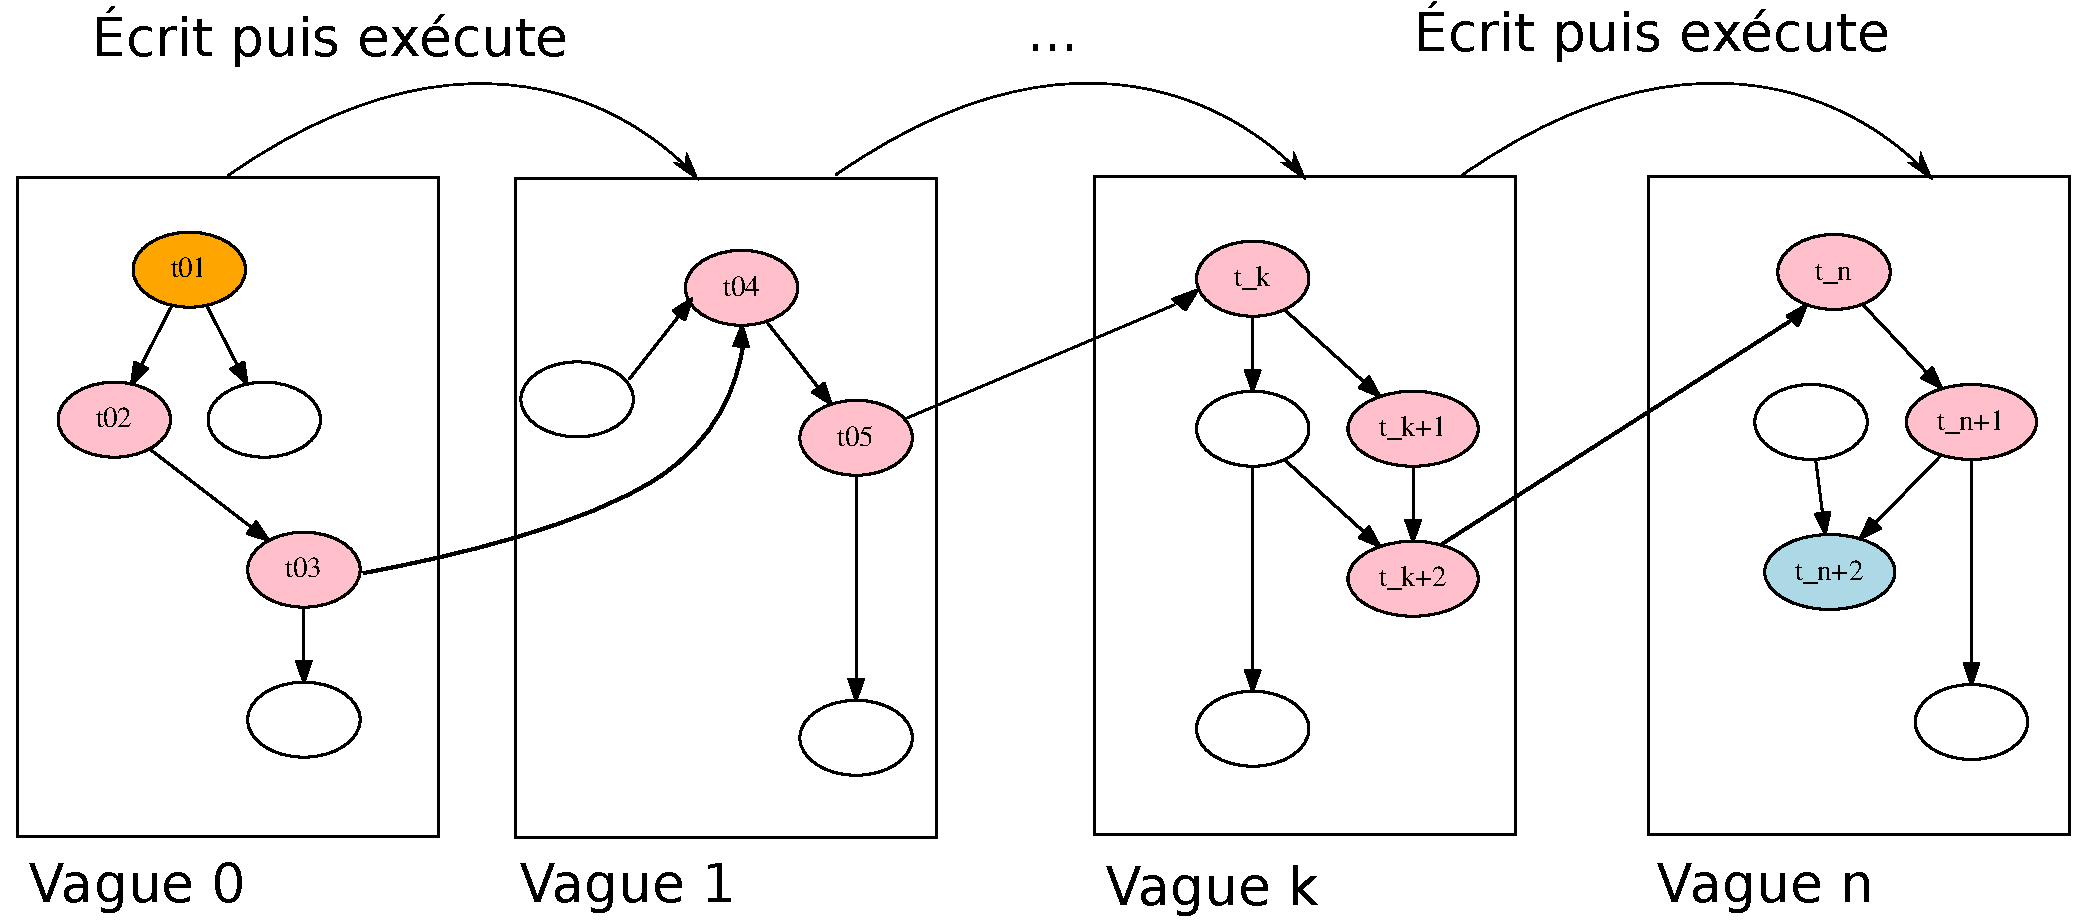
\includegraphics[width=1.0\textwidth]{supports/automodification/phases2_final.pdf}
 \caption{Vision informelle des vagues}
 \label{fig:vagues_visuel}
\end{figure}

\section{Trace, niveaux d'exécution et vagues}
Le programme exécuté a pour sources principales de données les registres et la mémoire constituée de la pile et du tas qui sont tous les deux adressables par des entiers. Une variable d'un programme est donc soit un registre du processeur soit une adresse mémoire, de même que défini dans la sémantique du langage intermédiaire défini au chapitre précédent (définition \ref{def:sem_conc_var}).

En utilisant la sémantique concrète précédemment définie on est capable, à partir d'un ensemble de valeurs initiales pour les registres et la mémoire, d'exécuter un programme sur cette entrée.
Schématiquement, l'exécution d'un programme consiste en la définition d'un contexte d'exécution initial $E_0$, l'évaluation sémantique de la première instruction $D_1$ dans ce contexte, puis l'évaluation de l'instruction suivante dans le contexte mis à jour, et ainsi de suite. Dans cette partie nous définirons formellement ces éléments mais leur enchaînement est schématiquement le suivant.

% \begin{figure}
\begin{center}
\scalebox{1}{
\begin{tikzpicture}[->,scale=1,>=stealth',thick]
\node[state, draw=none] (E0){$E_0$};
\node[state, draw=none, right=2cm of E0] (E1){$E_1$};
\node[state, draw=none, right=2cm of E1] (E2){$E_2$};
\node[state, draw=none, right=2cm of E2] (EP){$...$};
\node[state, draw=none, right=2cm of EP] (EN){$E_n$};
\draw (E0.east) -> node[above]{$D_1$} (E1.west);
\draw (E1.east) -> node[above]{$D_2$} (E2.west);
\draw (E2.east) -> node[above]{...} (EP.west);
\draw (EP.east) -> node[above]{$D_n$} (EN.west);
\end{tikzpicture}
}
\end{center}
% \caption{Enchaînement des contextes d'exécution et des instructions dynamiques}
% \label{fig:mem_process}
% \end{figure}

Nous rappelons que nous notons, à tout instant durant l'exécution, $\BT$ le tableau contenant les adresses mémoires et $\Theta$ le store représentant l'état des variables (mémoire et registres), comme indiqué aux définitions \ref{def:sem_conc_var} et \ref{def:sem_store_dynamique}.
Nous définissons une instruction dynamique (définition \ref{def:ensembles_inst_dyn}) par son adresse, les adresses mémoires sur lesquelles elle est codée et l'instruction machine correspondant. Ces informations sont données par le décodage d'une instruction à l'adresse mémoire spécifiée dans un contexte donné. 

\begin{defi}
On note $D$ une instruction dynamique constituée des éléments suivants.
\begin{itemize}
 \item \da{D} l'adresse mémoire de l'instruction dynamique
 \item \dc{D} l'intervalle des adresses mémoire sur lequel $D$ est codée
 \item \di{D} l'instruction machine à l'adresse \da{D}
%  \item \dr{D_i} l'ensemble des variables sur lesquelles l'exécution de \di{D_i} provoque une lecture
%  \item \dw{D} l'ensemble des variables sur lesquelles l'exécution de \di{D} provoque une écriture
\end{itemize}
On définit l'opérateur \texttt{decode} qui associe à une adresse mémoire $a$ et un store $\Theta$ l'instruction dynamique $D=$\texttt{decode}$(a, \Theta)$ présente à l'adresse $a$.
\label{def:ensembles_inst_dyn}
\end{defi}

Si l'on dispose d'un langage intermédiaire comme défini au chapitre précédent, son opérateur de désassemblage atomique nous donne ces informations. Pour l'assembleur \xq, une instruction est codée au maximum sur 15 octets.
% Si on cherche à désassembler \telock\ à l'adresse \adr{0x01006e7a}, et qu'à l'adresse \adr{0x01006e7d} sont présents les octets suivant : $\Theta[0x01006e7d..0x01006e8b]=$ \texttt{eb ff c9 7f e6 8b c1 29 00 00 00 f3 aa 66 ab}, l'opérateur \texttt{decode} renvoie la première instruction dynamique D à cette adresse : il s'agit de l'instruction assembleur \di{D}=\texttt{jmp +1} (d'une taille de deux octets : \texttt{eb ff}) à l'adresse \da{D}=\adr{0x01006e7d}, codée sur l'intervalle d'adresses \dc{D}=[\adr{0x01006e7d}, \adr{0x01006e7e}].
Si on cherche à désassembler l'exemple précédent à l'adresse \adr{0x8048060} : à l'adresse \adr{0x8048060} sont présents les octets suivants : $\Theta[0x8048060..0x804806e]=$ \texttt{b8 6b 80 04 08 b8 6b 80 04 08 66 c7 40 06 02}, l'opérateur \texttt{decode} renvoie la première instruction dynamique D à cette adresse : il s'agit de l'instruction assembleur \di{D}=\texttt{mov eax, 0x8048076} (d'une taille de cinq octets : \texttt{b8 6b 80 04 08}) à l'adresse \da{D}=\adr{0x8048060}, codée sur l'intervalle d'adresses \dc{D}=[\adr{0x8048060}, \adr{0x8048064}].

Afin de pouvoir séparer la trace d'exécution selon le moment où chaque instruction a été écrite, nous définissons aussi, pour une instruction dynamique et un store $\Theta$, l'ensemble des adresses mémoire sur lesquelles l'instruction elle provoque une écriture (définition \ref{def:ensembles_inst_dyn_write}).

\begin{defi}
Soit $D$ une instruction dynamique et $\Theta$ un store représentant l'état des variables (mémoire et registres). On note \dww{\Theta}{D} l'ensemble des adresses mémoire sur lesquelles l'exécution de $D$ provoque une écriture.
\label{def:ensembles_inst_dyn_write}
\end{defi}

Cette information est donnée par la sémantique concrète choisie : si l'instruction assembleur \di{D} est sémantiquement équivalente, avec le store $\Theta$, à la suite d'instructions atomiques $d_1, ..., d_n$ dans un langage intermédiaire alors l'ensemble des adresses écrites par D est l'union de adresses écrites par chacune des instructions atomiques $d_i$ dans la sémantique concrète choisie pour ce langage intermédiaire (propriété \ref{propri:eq_W_D_di}).

\begin{propri}
Soit $D$ une instruction dynamique, $\Theta$ un store représentant l'état des variables (mémoire et registres) et $d_1, ..., d_n$ une suite d'instruction atomiques dans un langage intermédiaire telle que la suite d'instruction $d_1, ..., d_n$ dans le langage intermédiaire est sémantiquement équivalente à l'instruction assembleur \di{D}. On a :
$$\mdww{\Theta}{D}=\mdww{\Theta}{d_1,..., d_n}=\mdww{\Theta}{d_1}\ \cup\ ...\ \cup\ \mdww{\Theta}{d_n}.$$
\label{propri:eq_W_D_di}
\end{propri}

Avec la sémantique définie au chapitre précédent les seules instructions qui provoquent des écritures sont celles dont la liste d'instructions atomiques donnée par le désassemblage contiennent des assignations écrivant, par adressage direct ou indirect, à une adresse mémoire $m$. Si \di{D} est une instruction assembleur sémantiquement équivalente, avec le store $\Theta$, à l'enchaînement des instructions atomiques $d_1, ..., d_n$ dans le langage intermédiaire précédent, alors \dww{\Theta}{D}=\dww{\Theta}{d_1}$\ \cup\ ...\ \cup\ $\dww{\Theta}{d_n} (propriété \ref{propri:eq_W_D_di}) avec
% \\
$$\mdww{\Theta}{d_i}=
\left\{
  \begin{array}{ll}
	  m &$ si $d_i=m\leftarrow g(x_1, ..., x_k)\ et\ m\in\BT
	\\\Theta(v) &$ si $d_i=[v]\leftarrow g(x_1, ..., x_k)\ et\ \Theta(v)\in\BT
	\\ \emptyset &$ sinon.$
  \end{array}
\right.
$$

% \begin{defi}
% Nous définissons le niveau d'écriture d'une adresse mémoire comme un entier naturel et le store $W^M: \BT\rightarrow\BN$ associant à une adresse mémoire son niveau d'écriture.
% \label{def:store_mem}
% \end{defi}

Nous définissons plus formellement la notion de contexte d'exécution (définition \ref{def:contexte_exec}) comme la donnée d'un niveau d'exécution, d'un store contenant les valeurs de la mémoire et des registres et d'un store contenant les niveaux d'écriture courants de chaque adresse mémoire.

\begin{defi}
Un contexte d'exécution est la donnée d'un triplet $E=(X, \Theta, W^M)$ où
\begin{itemize}
 \item $X\in\BN$ est le niveau d'exécution du contexte
 \item $\Theta$ est le store des valeurs du contexte, associant une valeur à chaque registre et chaque adresse mémoire
 \item $W^M$ est le store des niveaux d'écriture du contexte, associant à chaque adresse mémoire un niveau d'écriture dans $\BN$
\end{itemize}
Une exécution d'un programme, dont le point d'entrée est $ep$, est la donnée d'une suite finie de contextes d'exécution $E_0, E_1, ..., E_n$ tel que :
\begin{itemize}
 \item $X_0=1$, $\Theta_0[eip]=ep$ et $\forall m\in \BT, W_0^M[m\leftarrow 0]$
 \item En notant $D_{i+1}=$\texttt{decode}$(\Theta_i[eip], \Theta_i)$ l'instruction dynamique exécutée lors de la transition entre le contexte $E_i$ et $E_{i+1}$, on a :
    \begin{itemize}
     \item Le niveau d'écriture de $D_{i+1}$ est le niveau d'écriture maximum des octets qui la composent : $W_D=max(\{W^M[m],\ m\in\ $\dc{D_{i+1}}$\})$
     \item $X_{i+1}=max(X_i, W_D+1)$
     \item $\Theta_{i+1}$ est $\Theta_i$ mis à jour par l'évaluation sémantique de \di{D}
     \item $W_{i+1}^M=W_{i}^M$ sauf pour les adresses mémoire écrites par $D_{i+1}$:\\ $\forall m\in\ $\dw{D_{i+1}}$,\ W_{i+1}^M[m\leftarrow X_i]$
    \end{itemize}
\end{itemize}
\label{def:contexte_exec}
\end{defi}

Une exécution consiste en une série de contextes d'exécution dont la transition de l'un au suivant est provoquée par l'évaluation sémantique de l'instruction pointée par le registre de compteur ordinal (noté en général \pc\ ou \eip\ en assembleur \xq). Une trace d'exécution est une signature d'une exécution, elle contient les instructions successives avec leurs niveau d'exécution respectifs (définition \ref{def:trace}).

\begin{defi}
Étant donnée une exécution d'un programme composée des contextes d'exécution $E_0, E_1, ..., E_n$ avec $E_i=(X_i, \Theta_i, W_i^M)$, on appelle trace d'exécution la suite $T=(t_1, t_2, ..., t_n)$ où $t_i=(i, X_{i-1}, D_i)$ avec $D_i=$\texttt{decode}$(\Theta_{i-1}[eip], \Theta_{i-1})$.
\label{def:trace}
\end{defi}

Nous avons donc, pour une exécution donnée, des niveaux d'exécution successifs $1, 2, ..., n$.
À chaque contexte d'exécution, toute adresse en mémoire $m$ a un niveau d'écriture $W^M[m]$ correspondant au dernier niveau d'exécution durant lequel une instruction a modifié la valeur à l'adresse $m$.
Une instruction $D$ a un niveau d'écriture $W_D$ qui est le niveau d'écriture le plus élevé parmi les adresses sur lesquelles elle est codée.
Lors d'une exécution le niveau d'exécution ainsi que le niveau d'écriture de chaque adresse mémoire sont croissants.


% \begin{defi}
% Nous définissons une trace d'exécution comme la donnée d'une suite $T=t_1, t_2, ..., t_n$ composée de triplets de la forme $t_i=(i, D_i, X_i)$ tels que
% \begin{itemize}
%  \item $D_i$ est la $i^{eme}$ instruction dynamique exécutée.
%  \item Avant l'exécution de l'instruction $D_i$, le niveau d'exécution est \texttt{$X_{i-1}$}.
%  \item Après l'exécution de l'instruction $D_i$, le niveau d'exécution est \texttt{$X_i$}.
% \end{itemize}
% \label{def:write_exec_levels}
% \end{defi}



% \begin{propri}
%  Si le niveau d'exécution courant est $X$, le niveau d'exécution de l'instruction à exécuter $D_i$ est :\\
%  $X=max(X, W_D+1)$ avec $W_D=max(W^M[a],\ a\in\ $\dc{D_i}$)$.\\
%  Après l'exécution de $D_i$, les niveaux d'écriture dans la mémoire sont mis à jour de la manière suivante :\\
%  $\forall a\in$ \dw{D_i}, $W^M[a]=X$.
% \label{propri:niveau_exec}
% \end{propri}

En pratique une instruction $D$ écrite par une instruction ayant pour niveau d'exécution $k$ puis directement exécutée aura pour niveau d'écriture $W_D=k$ et pour niveau d'exécution $X=k+1$. On définit alors un instantané du niveau d'exécution $k$ selon la définition \ref{def:instantane} et une vague comme étant le désassemblage parfait de cet instantané (définition \ref{def:vagues}).

\begin{defi}
 Étant donnée une exécution d'un programme composée des contextes d'exécution $E_0, E_1, ..., E_n$ avec $E_i=(X_i, \Theta_i, W_i^M)$, on appelle instantané du niveau d'exécution $k$ l'état de la mémoire contenu dans $\Theta_j$ où $E_j$ est le premier contexte d'exécution dont le niveau d'exécution est $X_j=k$.
 On appelle point d'entrée et point de sortie de cet instantané respectivement $D_{in}=$\texttt{decode}$(\Theta_{j}[eip], \Theta_{j})$ et  $D_{out}=$\texttt{decode}$(\Theta_{l}[eip], \Theta_{l})$ où $E_l$ est le dernier contexte d'exécution dont le niveau d'exécution est $X_l=k$.
 \label{def:instantane}
\end{defi}

\begin{defi}
 Étant donnée une exécution d'un programme, on appelle vague $k$ le graphe de flot de contrôle parfait du programme représenté par l'instantané du niveau d'exécution $k$ muni de son point d'entrée.
 \label{def:vagues}
\end{defi}

Une première vague est définie dès l'exécution de la première instruction du programme puis à chaque changement de niveau d'exécution une nouvelle vague est construite.
L'algorithme \ref{algo:analyse_dyn_vagues} permet d'exécuter un programme dynamiquement avec la sémantique concrète choisie tout en déterminant les niveaux d'exécution de d'écriture au fur et à mesure de l'exécution. 
Il fournit en sortie la trace d'exécution et la liste des vagues reconstruites.

\begin{figure}[h]
\begin{center}
\begin{tabular}[b]{|l|l|l|l|l|l|l|}
\hline
i & \da{D_i} & \dc{D_i} & \di{D_i} & \dw{D_i} & $W^\Theta_i$ & $X_i$ \\
\hline
1 & 8048060  & [8048060, 8048064] & mov    eax, 0x8048076  &           & 0 & 1 \\
2 & 8048065  & [8048065, 804806a] & mov    [eax+1], 2      & 0x8048077 & 0 & 1 \\
3 & 804806b  & [804806b, 8048075] & mov    [eax+6], 2      & 0x804807c & 0 & 1 \\
4 & 8048076  & [8048076, 804807a] & mov    edi, 1          &           & 1 & 2 \\
5 & 804807b  & [804807b, 804807f] & mov    ebx, 1          &           & 1 & 2 \\
\hline
\end{tabular}
\end{center}
\caption{Trace d'exécution du programme auto-modifiant de la figure \ref{fig:prg_asm_sm}}
\label{fig:prg_asm_sm_trace}
\end{figure}

Reprenons l'exemple du programme \sm\ précédent.
La figure \ref{fig:prg_asm_sm_trace} donne une trace d'exécution de ce programme en détaillant les informations sur chaque instruction dynamique ainsi que les niveaux d'écriture et d'exécution de chaque instruction.
Au départ toute la mémoire est dans son état d'origine et a pour niveau d'exécution 0. Lorsque l'instruction $D_1$ est exécutée, il n'y a pas eu d'auto-modification donc le niveau d'écriture est 0 et le niveau d'exécution est 1.
Les instructions $D_2$ et $D_3$ provoquent une auto-modification : les octets aux adresses \adr{0x8048077} et \adr{0x804807c} sont modifiés et leurs niveaux d'écriture deviennent donc le niveau d'exécution courant, soit 1.
Lorsque l'exécution atteint $D_4$, qui a été modifié, le niveau d'écriture est 1 donc le niveau d'exécution devient 2.
L'instruction suivante $D_5$ a également un niveau d'écriture de 1 donc le niveau d'exécution est inchangé.

Cette exécution est donc séparée en deux vagues : la vague initiale, $v_0$ dont l'instantané est l'état de la mémoire avant l'exécution de la première instruction et la vague $v_1$ contenant l'état de la mémoire juste après l'exécution de $D_3$ et avant l'exécution de la première instruction modifiée $D_4$.


% \begin{figure}
% \begin{center}
% \begin{tabular}[b]{|l|l|l|l|l|l|l|}
% \hline
% i & \da{D_i} & \dc{D_i} & \di{D_i} & \dw{D_i} & $W_i$ & $X_i$ \\
% \hline
% & 8048060  &  (...)         	        & Pile -> RWX &  & 0 & 1 \\ 
% 1 & 804807c  &  [804807c, 8048080]         &  mov    edi, 0x0 & edi & 0 & 1 \\
% 2 & 8048081  &  [8048081, 8048086]         &  mov    eax, 0x8048091 & eax & 0 & 1 \\
% 3 & 8048086  &  [8048086, 804808a]         &  mov    [eax], 0xeb & 0x8048091 & 0 & 1 \\
% 4 & 804808b  &  [804808b, 8048090]         &  mov    [eax+1], 0x7 & 0x8048092 & 0 & 1 \\
% 5 & 8048091  &  [8048091, 8048092]         &  jmp    80480a1 <edi3> &  & 1 & 2  \\
% 6 & 804809a  &  [804809a, 804809d]         &  mov    edi,0x2 & edi & 0 & 2\\
% 7 & 804809f  &  [804809f, 80480a0]         &  jmp    80480a8 <fin> &  & 0 & 2\\
%  & 80480a8  &  (...)		        &  Affiche edi &  & 0 & 2\\
%  & 80480c3  &  (...)		        &  Quitte &  & 0 & 2\\
% \hline
% \end{tabular}
% \end{center}
% \caption{Trace d'exécution du programme auto-modifiant de la figure \ref{fig:unevague_v0}}
% \label{fig:unevague_trace}
% \end{figure}

\begin{algorithm}[h] %or another one check
\caption{Mise à jour du niveau d'exécution d'une instruction}
\SetAlgoLined
\KwIn{La mémoire, l'opérateur de niveau d'écriture, une instruction dynamique et le niveau d'exécution courant}
\KwResult{Le niveau d'exécution courant mis à jour}
\SetKwProg{Fn}{}{}{}
\SetKwFunction{FRecurs}{MAJExecution}
\Fn(
){\FRecurs{M, $W^M$, D, X}}{
$W_D \leftarrow\ max(W^M[a],\ a\in\ $\dc{D}$)$\\
$X \leftarrow\ max(X,\ W_D+1)$ \\
\Return X
}
\label{algo:update_exec_level}
\end{algorithm}

\begin{algorithm}[h] %or another one check
\caption{Mise à jour des niveaux d'écriture lors de l'exécution d'une instruction}
\SetAlgoLined
\KwIn{La mémoire, l'opérateur de niveau d'écriture, une instruction dynamique et le niveau d'exécution courant}
\KwResult{L'opérateur de niveau d'écriture mis à jour}
\SetKwProg{Fn}{}{}{}
\SetKwFunction{FRecurs}{MAJEcriture}
\Fn(
){\FRecurs{M, $W^M$, D, X}}{
\For {$m\in\ $\dw{D}}{
  $W^M[m]\leftarrow\ X$
}
\Return $W^M$
}
\label{algo:update_write_level}
\end{algorithm}

\begin{algorithm}[H] %or another one check
\caption{Analyse dynamique avec calcul des vagues}
\SetAlgoLined
\KwIn{Les registres R et une mémoire M dans laquelle un programme de point d'entrée \texttt{ep} a été chargé}
\KwResult{La trace des instructions dynamiques chacune associée à leur niveau d'exécution et les différentes vagues de la trace}
\SetKwProg{Fn}{}{}{}
\SetKwFunction{FRecurs}{analyseDynamique}
\Fn(
% \tcc*[h]{C : matrice des associations possibles, i : numéro du prochain sommet de P à associer, F : liste des couples d'associations déjà faites}
){\FRecurs{R, M, ep}}{
\For{$m\in M$}{
  $W^M[m]\leftarrow 0$\\
}
$(X, X_{-1}, i, T, instantanes, eip)\leftarrow (1, 0, 1, \emptyset, \emptyset, ep)$\\
% $X\leftarrow 1$\\
% $X_{-1}\leftarrow 0$\\
% $i\leftarrow 0$\\
% $T\leftarrow \emptyset$\\
% $vagues\leftarrow \emptyset$\\
% $eip\leftarrow ep$\\
\While {la fin du programme n'est pas atteinte}{
\tcc{Le programme est exécuté en prenant l'instruction suivante à l'adresse eip}
$D\leftarrow decode(eip, M)$\\
$X\leftarrow MAJExecution(M, W^M, D, X)$\\
\If {$X \ne X_{-1}$}{
  \tcc{Quand le niveau d'exécution change, on prend un instantané de la mémoire}
  $instantanes\leftarrow instantanes\cup \{(X_{-1}, M)\}$
}
$X_{-1} \leftarrow X$\\
~\\
\tcc{On met à jour le contexte à partir de l'instruction courante en l'évaluant sémantiquement}
$(eip, R, M)\leftarrow sem\_eval(eip, R, M)$\\
$W^M\leftarrow MAJEcriture(M, W^M, D, X)$\\
$T\leftarrow T\cup\{(i, X, D_i)\}$\\
$i\leftarrow i+1$\\
}
\Return T, instantanes
}
\label{algo:analyse_dyn_vagues}
\end{algorithm}

\begin{rem}
 Étant donné la définition croissante des niveaux d'exécution, une instruction dynamique peut-être exécutée non seulement plusieurs fois au même niveau d'exécution mais également être présente à des niveaux d'exécution différents.
\end{rem}

\section{Revue de littérature}
La notion de vague présentée dans ce chapitre a été développée dans les thèse de Reynaud \cite{Reynaud2010} et Calvet \cite{Calvet2013}.
Elle est similaire à la notion de \emph{phase} présentée par Debray et Patel \cite{DP10} et utilisée pour automatiser la suppression de la protection d'un binaire. Le découpage d'une trace en phases est, chez eux, identique au découpage en vagues que l'on présente dans ce chapitre.
En particulier le programme auto-modifiant précédent (figure \ref{fig:prg_asm_sm}), exécuté, forme deux vagues : la vague initiale est le programme initial et la seconde, modifiée, est identique à l'exception des instructions 4 et 5 qui ont été modifiées en \texttt{mov edi, 2} et \texttt{mov ebx, 2} respectivement.
En général la suppression des protections se fait à l'aide d'une analyse dynamique et d'une image de la mémoire à un instant donné au cours de l'exécution. C'est cette image mémoire qui sera considérée comme étant le programme d'origine. La difficulté réside alors dans le choix de l'instant où prendre l'image mémoire : il s'agit souvent la dernière phase.

Preda, Giacobazzi, Debray, Coogan et Townsend \cite{PGDCT10} effectuent un découpage en phases mais chaque exécution d'une instruction écrite lors d'une vague précédente (pas uniquement lors de la phase en cours) provoque la création d'une nouvelle phase.
Avec l'exemple précédent, leur approche crée trois phases : la phase initiale, celle où uniquement l'instruction 4 a été modifiée, puis celle où les instructions 4 et 5 ont été modifiées.

\section{Implémentations}
Plusieurs choix s'offrent à qui cherche à implémenter un système d'analyse dynamique de binaire tels l'émulation, l'instrumentation et le débogage.

L'émulation consiste à lancer l'exécution dans un environnement d'exécution simulé, qui peut être un système d'exploitation complet comme c'est le cas avec BAP ou TEMU, le module d'analyse dynamique du projet BitBlaze \cite{bitblaze08}, basé sur l'émulateur QEMU \cite{QEMU05}.

On instrumente un binaire exécuté en y insérant, généralement au cours de son exécution, du code assembleur servant à son analyse. Intel développe PinTools \cite{pintools} pour l'analyse de programmes tournant sur leurs processeurs.

Enfin le débogage suit pas à pas l'exécution d'un programme en utilisant le drapeau de trappe (\emph{Trap Flag}), permettant de reprendre la main après chaque instruction du programme débogué afin d'examiner son environnement d'exécution.
\\

Le débogage comme l'instrumentation n'utilisent pas de langage intermédiaire tandis qu'un émulateur tel que BAP transcrit d'abord les instructions dans son langage intermédiaire pour les exécuter avec la sémantique concrète du langage intermédiaire.
L'émulation est donc intéressante parce qu'à aucun moment le programme analysé n'a un accès libre au système sur lequel il s'exécute.
La limitation est donc que les interactions du programme émulé avec le système d'exploitation visé sont restreintes.
En particulier les appels systèmes, qui ne sont pas transcrits par BAP, ne peuvent pas être émulés directement, rendant l'analyse très partielle.
Les approches nécessitant une exécution non restreinte sur le système sont alors réalisées au sein d'une machine virtuelle.

Une caractéristique cruciale d'un analyseur dynamique est qu'il doit être transparent : le programme analysé ne doit pas être capable de différencier son exécution dans l'analyseur de son exécution sur un système réel.
Cette transparence est en général partielle, que ce soit avec un émulateur, un débogueur ou une technique d'instrumentation. \more{cite blue pill ou autre}

L'instrumentation, par rapport au débogage, offre des performances temporelles d'exécution bien supérieures.
Pour ces raisons, nous nous sommes intéressés à l'émulation comme à l'instrumentation.
\\

L'émulation permet une analyse plus abstraite et nous avons développé un analyseur partiel de programmes auto-modifiants basé sur BAP.
L'instrumentation permet d'exécuter plus fidèlement le programme à analyser, nous avons donc principalement favorisé cette approche pour l'analyse de programmes malveillants. Nous avons choisi Pin qui, sans fournir de sémantique concrète pour l'assembleur, permet d'obtenir d'une instruction dynamique l'ensemble des adresses sur lesquelles elle écrit, comme souhaité à la définition \ref{def:ensembles_inst_dyn_write}.

\subsection{Émulation avec BAP}
Nous avons repris l'implémentation d'un émulateur pour programmes \sms\ basée sur BAP présentée au chapitre \ref{chap:semantique} et avons ajouté la séparation de la trace en plusieurs vagues d'exécution, selon l'algorithme \ref{algo:analyse_dyn_vagues}.

Cette implémentation donne le résultat attendu avec des programmes simples et qui n'utilisent pas d'appels système.
Sur l'exemple de programme \sm\ donné en début de chapitre, la sortie est la suivante.
L'exécution, de la première (\emph{pc: 1}) à la dernière instruction, est correctement découpée en vagues et les instructions correspondent à celles modifiées lors de l'exécution.

\begin{center}
\begin{verbatim}
Vague 1, pc: 1: addr 0x8048060 @asm "mov    eax, 0x8048071"
Vague 1, pc: 2: addr 0x8048065 @asm "movw   [eax+1], 2"
Vague 1, pc: 3: addr 0x804806b @asm "movw   [eax+6], 2"
Vague 2, pc: 4: addr 0x8048071 @asm "mov    edi, 2"
Vague 2, pc: 5: addr 0x8048076 @asm "mov    ebx, 2"
\end{verbatim}
\end{center}

Ne pouvant pas émuler des programmes utilisant des appels systèmes, nous avons laissé de coté cette approche pour une approche par instrumentation permettant l'analyse de programmes réels.


\subsection{Instrumentation avec Pin}
\itodo{tracesurfer?}
Pin est l'outil d'instrumentation développé par Intel pour ses processeurs \xq\ et \xs.
Il fournit un niveau d'information sémantique de niveau 2, donc suffisant pour suivre chaque instruction et connaître l'ensemble des adresses mémoire que l'instruction modifie. 
Nous avons repris l'implémentation de l'algorithme \ref{algo:analyse_dyn_vagues} développé par Reynaud \cite{Reynaud2010} sous la forme d'un PinTool : codé en C, il s'agit d'un programme définissant les actions à effectuer avant et après l'exécution de chaque instruction selon le type de l'instruction considérée.

L'analyse d'un programme malveillant a lieu sur une machine virtuelle munie de Pin et ne souffre pas des limitations de l'émulation : les appels systèmes sont correctement analysés et exécutés. 
Dans la suite de cette thèse, nous avons exclusivement utilisé cette approche pour l'analyse dynamique.



\DontFrameThisInToc
\chapter{Désassemblage d'un programme \sm\label{chap:desassembleur}}


% \section{Analyse dynamique et auto-modification}
% L'analyse dynamique consiste donc à se baser sur une ou des exécutions particulières d'un programme pour inférer des propriétés sur son fonctionnement.
% Elle demande donc de se munir d'une langage modélisant le fonctionnement de la machine durant l'exécution du programme, d'une sémantique concrète de l'assembleur utilisé et de lancer l'évaluation sémantique du programme sur une ou plusieurs entrées.
% Les entrées d'un programme sont par exemple les paramètres passés lors de l'appel au programme, l'état de la machine lors du démarrage, les données lues depuis la mémoire et les saisies faites par l'utilisateur au clavier ou à la souris lors de l'exécution s'il s'agit d'une application dotée d'une interface graphique.
% Dans cette partie nous reprendrons la sémantique simplifiée pour un langage assembleur définie au chapitre précédent et expliquerons comment séparer une exécution d'un programme auto-modifiant en plusieurs sous-exécution non auto-modifiantes afin d'utiliser des techniques standard d'analyse sur chacune de ces sous-exécutions.

Nous avons précédemment détaillé plusieurs techniques d'obscurcissement de code. 
Nous avons décrit des méthodes d'analyse de programmes \nsm\ présentant des chevauchements de code et une méthode permettant de ramener l'analyse d'un programme \sm\ à l'analyse de plusieurs programmes \nsms\ par découpage en instantanés.

Dans ce chapitre nous présentons une méthode d'analyse combinant l'approche dynamique pour gérer les programmes \sms\ et une analyse statique de chaque sous programme considéré à partir d'un instantané et de la trace d'exécution.

\section{Désassemblage parfait}
% \subsection{}
Nous avons, au chapitre \ref{chap:assembleur}, défini le désassemblage parfait d'un programme \nsm\ comme la donnée de l'ensemble des adresses auxquelles des instructions peuvent être atteintes lors de l'exécution.
Dans le cas d'un programme \sm, cette définition n'est pas suffisante puisque l'instruction présente à une adresse dépend du contexte d'exécution et des éventuelles modifications qui ont été faites à cette adresse.

Nous considérons toujours que la donnée que l'analyste cherche à
déterminer et représenter est l'ensemble des exécution possibles du
programme : nous notons $E_T$ l'ensemble des traces d'exécution possibles.
En particulier une entrée spécifique provoque une exécution que nous observons sous la forme d'une trace.
Cette trace peut être découpée en niveaux d'exécution et chaque vague est le désassemblage parfait de l'instantané.

Le désassemblage, pris au sens de l'opération inverse de l'assemblage,
consiste à déterminer les adresses contenant des instructions, les
autres contenant des données.
Au sein d'une exécution les octets sur lesquelles une instruction ayant
un niveau d'exécution strictement supérieur à 1, c'est à dire que ces
octets ont été modifiés avant que l'instruction ne soit exécutée, ne
sont présents dans la représentation d'origine du programme qu'en temps
que données.
Ainsi le désassemblage parfait d'un programme \sm\ ne prend en compte
que les instructions exécutées avec un le niveau d'exécution 1
(proposition \ref{prop:desassemblage_parfait_sm}).

\begin{prop}
 Étant donné un programme P \sm\ et l'ensemble de ses traces d'exécution
$E_T$, le désassemblage parfait de P est l'ensemble des adresses où une
instruction de niveau d'exécution 1 est exécutée dans au moins une
trace, c'est à dire
 $\{a, \exists\ T\in E_T, \exists\ (i, X, D)\in T, X=1,\ $\da{D}$=a\}$.
\label{prop:desassemblage_parfait_sm}
\end{prop}


\subsection{Graphe de flot de contrôle parfait}
Le graphe de flot de contrôle ne peut plus se contenter de représenter
une instruction par son adresse puisque plusieurs instructions
différentes peuvent être présentes à la même adresse.
Le graphe de flot de contrôle parfait est alors le graphe dont les
sommets sont des couples $(a, I)$ où \adr{a} est une adresse et $I$ une
instruction assembleur. Il y a un arc entre deux sommets si le second
suit directement le premier dans une trace d'exécution (définition
\ref{def:cfg_parfait_sm}).

\begin{defi}
 Étant donné un programme \sm\ P et l'ensemble de ses traces d'exécution
$E_T$, le graphe de flot de contrôle parfait de P est le graphe orienté
$G=(V, E)$ tel que :
 \begin{itemize}
  \item $V=\{(\mda{D}, \mdi{D}),  (i, X, D)\in E_T\}$
  \item $((a_1, I_1), (a_2, I_2))\in E\ si\ et\ seulement\ si\ (a_1,
I_1)\ et\ (a_2, I_2)\ se\ suivent\ dans\ une\ trace\ : \exists T\in
E_T,\ i\in \BN, (i, X_1, D_1)\ et\ (i+1, X_2, D_2)\in T\ avec\
$\da{D_1}$=a_1,\ $\di{D_1}$=I_1,$~\da{D_2}$=a_2,\ $\di{D_2}$=I_2$.
 \end{itemize}
\label{def:cfg_parfait_sm}
\end{defi}

Le problème de cette définition d'un GFC pour un programme \sm\ est qu'%e souvent les vagues se suivent et ont peu de rapport les unes avec les autres.
elle ne permet pas de visualiser l'enchaînement des vagues et peut conduire à une interprêtation biaisée des exécutions possibles.

\paragraph{Exemple.}
Prenons le programme donné en figure \ref{fig:sm_asm} dont le graphe de flot de contrôle construit par analyse statique à l'aide d'un parcours récursif est en figure \ref{fig:sm_cfg_statique}.

\begin{figure}[h]
\begin{center}
% \subfigure[]{
\begin{tabular}[b]{|l|l|l|l|}
\hline
Adresse & Octets & Instruction & Instruction écrite\\ 
\hline
 8048060 <debut>  &  31 ff             &  xor    edi,edi		& \\
 8048062  &  40                        &  inc    eax			& \\
 8048063  &  74 07                     &  je     804806c <si\_zero> 	& \\
 	  &			       &				& \\
 8048065  &  bf 02 00 00 00            &  mov    edi, 0x2 		& \\
 804806a  &  eb f4                     &  jmp    8048060 <debut> 	& \\
	  &			       &				& \\
 804806c <si\_zero> &  bf 01 00 00 00  &  mov    edi, 0x1 		& \\
 8048071  &  bb 60 80 04 08            &  mov    ebx, 0x8048060 	& \\
 8048076  &  66 c7 03 47 00            &  mov    [ebx], 0x47 		& inc edi\\
 804807b  &  66 c7 43 01 47 00         &  mov    [ebx+0x1], 0x47	& inc edi \\
 8048081  &  66 c7 43 03 c3 00         &  mov    [ebx+0x3], 0xc3	& ret \\
 8048087  &  eb d7                     &  jmp    8048060 <debut> 	& \\
\hline
\end{tabular}
\caption{Code \sm}
\label{fig:sm_asm}
\end{center}
\end{figure}

\begin{figure}[h]
\begin{center}
\includegraphics[width=0.8\textwidth]{supports/disas_sm/ex2_statique.pdf}
% \label{fig:sm_cfg_statique}
% }
\caption{GFC par analyse statique et récursive}
\label{fig:sm_cfg_statique}
\end{center}
\end{figure}

% \FloatBarrier

La branche du saut effectué à l'adresse \adr{0x8048063} dans le cas où \eax\ est différent de zéro revient vers le point d'entrée, incrémente \eax\ et passe à nouveau dans le saut conditionnel. Cette boucle provoquera à terme un dépassement d'entier sur la valeur \eax\ qui sera remise à zéro et l'autre branche du saut sera appelée.
Cette seconde branche a pour effet de modifier les instructions aux adresses \adr{0x8048060}, \adr{0x8048061} et \adr{0x8048063} pour y placer les instructions \texttt{inc edi}, \texttt{inc edi} et \texttt{ret} respectivement, puis de sauter sur l'adresse \adr{0x8048060}, provoquant l'exécution des instructions écrites ainsi que de l'instruction \texttt{inc eax}, non modifiée.

Ainsi toutes les exécutions possibles, paramétrées par la valeur initiale d'\eax, bouclent sur la branche conditionnelle un nombre fini, qui peut être nul, de fois et exécutent la seconde branche, qui met la valeur 1 dans \edi, provoque une auto-modification, incrémente \edi\ deux fois puis quitte la fonction. Dans toutes les exécutions possibles la valeur finale de \edi\ est toujours 3.

Le GFC parfait de ce programme est donné en figure \ref{fig:sm_cfg_parfait}. En raison du mélange des instructions à différents niveaux d'exécution, il n'est pas possible de distinguer les vagues d'exécution et un analyseur statique simple approxime la valeur de \edi\ à 2 ou 3.

\begin{figure}[h]
\begin{center}
  \includegraphics[width=0.7\textwidth]{supports/disas_sm/ex2_parfait.pdf}
\end{center}
\caption{GFC parfait}
\label{fig:sm_cfg_parfait}
\end{figure}



Cette difficulté n'est pas intrinsèque aux programmes \sm\ et provient du fait même que le graphe de flot de contrôle est sur une \sura\ de l'ensemble des exécutions possibles. Il est cependant exacerbé dans le cas des programmes \sm\ puisque souvent les vagues successives n'ont que peu de code commun entre elles et il n'est pas cohérent de les mélanger dans le CFG.

\FloatBarrier
\subsection{Graphe de flot de contrôle paramétré par une exécution}
Nous proposons une représentation du GFC basée sur une exécution particulière et son découpage en différents niveaux d'exécution.
Nous donnons la définition d'une exécution (définition \ref{def:execution}), issue du résultat de l'analyse dynamique définie au chapitre précédent. L'exécution d'un programme sur une entrée I est caractérisée, via l'algorithme \ref{algo:analyse_dyn_vagues}, par le couple $(T, S)$ où $T$ est une trace et $S$ une liste d'instantanés d'exécution, un pour chaque niveau d'exécution.

\begin{defi}
 Soit un programme P prenant une entrée et ayant pour point d'entrée $ep$.
 $(T, S)$ est une exécution de P si et seulement si il existe une entrée I telle que (T, S)=\texttt{exécution(P, I, ep)}.
 
 On note $E_X$ l'ensemble des exécutions de P : $E_X=\bigcup_I\{\texttt{exécution(P, I, ep)}\}$.
\label{def:execution}
\end{defi}

L'exécution choisie, dite de référence, consiste donc en une trace et un enchaînement d'instantanés de chaque niveau d'exécution.
Chaque instantané est pris comme un programme ayant pour point d'entrée la première instruction de la trace ayant le niveau d'exécution correspondant et un point de sortie étant la dernière instruction ayant ce même niveau d'exécution.

Nous appelons GFC paramétré par cette exécution l'union des GFC parfaits de chaque de ces instantanés dans lequel les sommets sont caractérisés par le niveau d'exécution de l'instantané, une adresse et une instruction assembleur.
Formellement cette définition est possible si l'on se restreint à vouloir construire le GFC des seules exécutions dont les instantanés sont identiques à ceux de l'exécution de référence, on dit alors que ces exécutions sont compatibles (définition \ref{def:executions_compatibles}).

\begin{defi}
 Soit un programme P et $(T, S)$ et $(T', S')$ deux exécutions de P.
 $(T, S)$ et $(T', S')$ sont dites compatibles si et seulement si $S=S'$.
\label{def:executions_compatibles}
\end{defi}

Le GFC paramétré (définition \ref{def:cfg_param_sm}) représente chaque instruction contenue dans une trace dont l'exécution est compatible avec l'exécution de référence comme un sommet en prenant en compte son niveau d'exécution, son adresse et l'instruction assembleur. Deux sommets sont reliés par un arc si, dans une trace d'une exécution compatible, leurs deux instructions se suivent immédiatement.

\begin{defi}
 Étant donné un programme P \sm, $(T, S)$ une exécution de P et $E_C$ l'ensemble des exécutions de P compatibles avec $(T, S)$.
 Nous appelons GFC paramétré par $T$ le graphe $G=(V, E)$ tel que :
 \begin{itemize}
  \item $V=\{(X,\ $\da{D}$,\ $\di{D}$), (i, X, D)\in T',\ (T', S')\in E_C \}$%\in E_C, \exists\ (i, X, D)\in T',\
%$\da{D}$=a,\ $\di{D}$=I\}$
  \item $((X_1, a_1, I_1), (X_2, a_2, I_2))\in E$ si et seulement si $(X_1, a_1,
I_1)\ et\ (X_2, a_2, I_2)$ se suivent dans une trace : $\exists (T', S')\in
E_C,\ i\in \BN, (i, X_1, D_1)\ et\ (i+1, X_2, D_2)\in T$ avec \da{D_1}$=a_1,\ $\di{D_1}$=I_1,$~\da{D_2}$=a_2,\ $\di{D_2}$=I_2$.
 \end{itemize}
\label{def:cfg_param_sm}
\end{defi}


Un tel GFC pour le programme \sm\ précédent est donné en figure \ref{fig:sm_cfg_vagues} : l'exécution prise en compte est celle démarrant avec \eax=-2. La boucle directe est exécutée une fois, puis comme \eax=0, la partie auto-modifiante est activée. Dans l'exemple choisi ici, toutes les exécution partagent le même découpage en vagues et le GFC est séparé en deux GFC partiels (définition \ref{def:GFC_partiel}), celui de la vague 1 et celui de la vague 2.

\begin{defi}
 On appelle GFC partiel paramétré par une exécution $(T, S)$ et un instantané du niveau d'exécution $X$ le GFC paramétré par $T$ restreint aux sommets dont le niveau d'exécution est $X$.
\label{def:GFC_partiel}
\end{defi}


% \begin{defi}
%  Étant donné un programme \sm\ P et une trace d'exécution $T$, le graphe de flot de contrôle de P paramétré par $T$ est $G=(V, E)$ tel que :
%  \begin{itemize}
%   \item $V=\{(a, I),  \exists\ T\in E_T, \exists\ (i, X, D)\in T,\
% $\da{D}$=a,\ $\di{D}$=I\}$
%   \item $((a_1, I_1), (a_2, I_2))\in E\ si\ et\ seulement\ si\ (a_1,
% I_1)\ et\ (a_2, I_2)\ se\ suivent\ dans\ une\ trace\ : \exists T\in
% E_T,\ i\in \BN, (i, X_1, D_1)\ et\ (i+1, X_2, D_2)\in T\ avec\
% $\da{D_1}$=a_1,\ $\di{D_1}$=I_1,$~\da{D_2}$=a_2,\ $\di{D_2}$=I_2$.
%  \end{itemize}
% \label{def:cfg_param_sm}
% \end{defi}

\begin{figure}[h]
\begin{center}
  \includegraphics[width=0.6\textwidth]{supports/disas_sm/ex2_vagues.pdf}
\end{center}
\caption{GFC paramétré par l'exécution démarrant avec \eax=-2}
\label{fig:sm_cfg_vagues}
\end{figure}


L'idée consiste donc à obtenir une exécution particulière d'un programme puis à augmenter la couverture de code à l'aide d'une analyse statique sur chaque instantané de l'exécution. Nous discuterons de la pertinence de cette approche.

\FloatBarrier
\subsection{Revue de littérature}
\itodo{renovo ?}
Anckaert, Madou et Bosschere \cite{AMB06} proposent d'introduire la représentation sous forme d'octets de chaque instruction au sein du graphe de flot de contrôle et d'ajouter aux arcs les conditions sur les octets en mémoire. Sur l'exemple précédent, leur GFC, présenté en figure \ref{fig:sm_cfg_parfait_amb}, est identique au GFC parfait mais il est alors possible de différencier les chemins selon l'état de la mémoire et donc plus précis pour une analyse automatique.
En fait le graphe qu'ils représentent est un automate, permettant de compléter la notion d'automate de flot de contrôle introduit comme extension au graphe de flot de contrôle \cite{HJMS02} pour des programmes \sms.

\begin{figure}[h]
\begin{center}
  \includegraphics[width=0.8\textwidth]{supports/disas_sm/ex2_parfait_amb.pdf}
\end{center}
\caption{GFC parfait augmenté des octets et des conditions de transition}
\label{fig:sm_cfg_parfait_amb}
\end{figure}

\FloatBarrier
\section{Approche hybride}
% Nous avons vu comment séparer une trace d'exécution en plusieurs sous-traces définissant des vagues d'exécution.
% Chaque sous trace, au sein d'une vague, ne présente pas d'auto-modification.
% Nous décidons alors d'effectuer, pour chaque vague, un désassemblage par analyse statique en séparant le code en plusieurs \layers. Cette analyse est pertinente si les vagues ne présentent pas d'auto-modification. Nous discuterons ce point\todo{todo}.

Notre objectif est donc de construire un GFC paramétré par une exécution représentative du programme à analyser.
L'analyse dynamique du programme est faite selon l'algorithme \ref{algo:analyse_dyn_vagues} du chapitre précédent et fournit une trace d'exécution générale et un découpage de l'exécution en plusieurs instantanés de la mémoire.
Nous obtenons les traces et les instantanés par instrumentation avec Pin comme indiqué au chapitre précédent.
L'architecture générale du désassembleur est donnée par la figure \ref{fig:diag_codisasm}.

% \subsection{Architecture générale}
\begin{figure}[h]
\begin{center}
\scalebox{1}{
\begin{tikzpicture}[->,scale=1,>=stealth',thick]
\newcommand\espace{0.3cm}
\node[state] (BIN){Binaire};
\node[state, above right=2cm and 3.8cm of BIN] (TRACE) {Trace};
\node[state, below=1.8cm of TRACE.west, anchor=west] (I0) {Instantané 0};
\node[state, below=3.0cm of TRACE.west, anchor=west] (I1) {Instantané 1};
\node[state, below=4.2cm of TRACE.west, anchor=west] (Ip) {Instantané ...};
\node[state, below=5.4cm of TRACE.west, anchor=west] (In) {Instantané n};
% \node[state, right=1.4cm  of BIN] (ASM){ASM};
% \node[state, right=1.4cm of ASM] (IR){LI};

\node[state, right=4cm of I0] (V0) {Vague 0};
\node[state, below=1.2 of V0.west, anchor=west] (V1) {Vague 1};
\node[state, below=2.4 of V0.west, anchor=west] (Vp) {Vague ...};
\node[state, below=3.6 of V0.west, anchor=west] (Vn) {Vague n};

\coordinate [right=2cm of BIN.east] (DYN);
\coordinate [right=1.6cm of TRACE.east] (C0);
\coordinate [right=0.5cm of C0] (C1);
\coordinate [right=0.5cm of C1] (Cp);
\coordinate [right=0.5cm of Cp] (Cn);
% \coordinate [above=0.1cm of C1] (C10m);
% \coordinate [below=0.1cm of C1] (C10p);
\draw [-] (TRACE.east) -- (C0);
\draw [-] (C0) -- (C1);
\draw [-] (C1) -- (Cp);
\draw [-] (Cp) -- (Cn);
\draw (C0) -- ($(C0)+(0, -1.8cm)$);
\draw (C1) -- ($(C1)+(0, -3cm)$);
\draw (Cp) -- ($(Cp)+(0, -4.2cm)$);
\draw (Cn) -- ($(Cn)+(0, -5.4cm)$);
% \draw (C1) -- (C10m);
% \draw (C10p) -- ($(C1)+(0, -1.8cm)$);
\draw [-] (BIN.east) -- node[below left=3.0cm and -3.2cm, text width=4cm](DYNAMIC){Analyse dynamique} (DYN);
\draw (DYN) |- (TRACE.west);
\draw (DYN) |- (I0.west);
\draw (DYN) |- (I1.west);
\draw (DYN) |- (Ip.west);
\draw (DYN) |- (In.west);
\draw (I0) -- (V0);
\draw (I1) -- (V1);
\draw (Ip) -- (Vp);
\draw (In) -- node[below right=0.5cm and -1.8cm, text width=4cm](STATIC){Analyse statique} (Vn);
\node [fit={($(V0.north west) + (-0.2, 0)$) ($(V1) + (0.0, 0)$) ($(Vp) + (0.0, 0)$) ($(Vn.south east) + (0.3, 0)$)}, draw, label=GFC paramétré par la trace] {};
\end{tikzpicture}
}
\end{center}
\caption{Architecture générale du désassembleur hybride}
\label{fig:diag_codisasm}
\end{figure}

\paragraph{Pertinence de l'approche.}
L'exécution à partir de laquelle on cherche à reconstruire le GFC se doit d'être représentative d'une exécution standard du programme sur une machine cible.
Dans le cas des programmes malveillants on tente donc de se faire passer pour une machine ciblée par l'attaquant pour laisser le programme mener son attaque. 
À part les informations provenant du système d'exploitation, un programme malveillant ne prend en général pas d'entrée et ne nécessite pas d'interaction avec l'utilisateur. Une seule exécution devrait donc permettre d'analyser son comportement.
D'autre part la plupart des logiciels malveillants sont compilés sans comportement auto-modifiant et sont ensuite empaquetés. C'est le binaire empaqueté qui est obscurcis et auto-modifiant.
Dans ce cas il est fréquent \cite{Calvet2013} que la charge utile, c'est à dire le binaire d'origine, ne soit activé qu'à la dernière vague de l'exécution.
Par conséquent c'est principalement le logiciel de protection qui peut empêcher l'exécution de référence d'être représentative en détectant que le programme est instrumenté, débogué ou émulé et en détournant l'exécution dans ce cas.

\itodo{citer des cas de détection}

% \subsection{Obtention des traces et des vagues}
\subsection{Analyse statique de chaque instantané}
Pour l'analyse statique nous disposons de la trace et des instantanés munis de leurs points d'entrée et sortie respectifs.
Nous cherchons, à partir de la trace et d'un instantané, à reconstruire la vague correspondante, c'est à dire le désassemblage parfait de l'instantané.
Nous appelons trace partielle la liste des éléments de la trace qui sont exécutés au même niveau d'exécution que l'instantané étudié.
Nous utilisons la trace partielle comme guide dans l'analyse de l'instantané. Toute instruction présente dans la trace est nécessaire du code et doit être inclue dans la vague et le GFC.

\paragraph{Reconstruction du GFC par parcours récursif.}
Nous effectuons un désassemblage par parcours récursif de l'instantané à partir de chaque instruction présente dans la trace partielle.
Dans le GFC partiel \todo{def} reconstitué, les instructions présentes dans la trace sont en rose, les autres en blanc. Le point d'entrée et le point de sortie sont colorés en orange et bleu clair respectivement.
Si deux instructions se suivent dans la trace alors l'arc dirigé les reliant provient de l'analyse dynamique et est plein. Si elles se suivent dans l'analyse récursive alors l'arc dirigé provient de l'analyse statique et est en pointillés. Un arc étant parcouru par l'analyse dynamique et statique est en gras. Les arcs en noir relie une instruction et l'instruction séquentielle suivante tandis que les arcs en noir représentent le saut d'un appel ou d'un saut (\call\ ou \jmp\ par exemple).

\paragraph{Point de sortie.}
La dernière instruction présente dans la trace partielle constitue le point de sortie de l'instantané.
Dans le cas où cette instruction n'est exécutées qu'une seule fois dans la trace partielle, c'est à dire que le changement de niveau d'exécution intervient dès qu'elle est exécutée la première fois, nous stoppons le parcours du programme après cette instruction en considérant que les instructions suivantes doivent être analysées dans l'instantané suivant.

\paragraph{Chemins invalides.}
Si tous les chemins d'exécution passant par une instruction $D$ aboutissent nécessairement sur une instruction provoquant une erreur, soit parce que son adresse n'est pas valide, soit parce qu'elle n'est pas une adresse \xq\ valide, alors l'instruction $D$ n'est pas valide non plus.
Nous n'incluons donc par ces instructions dans le GFC.
Une instruction dont les chemins aboutissent à un saut dont les cibles ne sont pas connues ne sont pas concernées puisqu'il est possible qu'une de ces cibles soit valide.


\paragraph{Mesure du chevauchement à l'aide des \layers.}
Nous utilisons le découpage cohérent en \layers\ adapté au parcours récursif défini à la section \ref{sec:layers_decoupage_recursif} du chapitre \ref{chap:chevauchement}.
Dans le GFC deux instructions qui se chevauchent sont liées par un arc noir non dirigé tracé en pointillés.


\paragraph{Construction des blocs de base.}
Dans les exemples de GFC déjà vus précédemment, nous avons regroupé certaines instructions dans le même bloc, dit bloc de base, lorsque le regroupement aide à la lisibilité et ne fait pas perdre d'informations. Nous regrouperons deux instructions $I_1$ et $I_2$ du GFC si et seulement si :
\begin{itemize}
 \item Elles se suivent séquentiellement : elles sont reliées par un arc dirigé de $I_1$ vers $I_2$ de couleur noire, et
 \item $I_1$ n'a pas d'autres arcs sortant que celui aboutissant sur $I_2$
 \item $I_2$ n'a pas d'autres arcs entrant que celui provenant de $I_1$
 \item $I_1$ et $I_2$ ne sont pas en chevauchement avec d'autres instructions
\end{itemize}



\section{Revue de littérature}


% \DontFrameThiswInToc
% \chapter{Analyse statique\label{chap:analyse-statique}}
% \todo[inline]{Objectifs : Code -> CFG + trouver tout le code possible}
\todo[inline]{Analyse statique : les possibilités et un exemple}

\paragraph{Découvrir exactement le code atteignable.}

\paragraph{Reconstruction du graphe de flot de contrôle.}


\section{Sémantique pour un langage de type assembleur}
\todo[inline]{Comment elle gère l'auto-modification, les layers ?}

\paragraph{Structure des variables et de la mémoire.}

\begin{defi}
On définit les symboles $x\in\BX$ comme constitués de variables $v\in\BV$ et de pointeurs $p\in\BP$ vers des variables. $\BV$ contient un ensemble fini de registres $a\in\BA$ et un tableau de taille finie $\mathbb{T}=\textlbrackdbl 0,\ t\textrbrackdbl$. Les éléments de $\BP$ sont des pointeurs vers une variable : $\{[v],\ v\in \BV\}$.
\end{defi}


\paragraph{Instructions et programmes.}
\begin{defi}
Des labels $l\in\BL$ numérotent les instructions où $\BL$ est un sous-ensemble fini de $\BN$ contenant $\bot$. Les instructions sont de ce type : \\
$inst:=\ $\emph{$x\leftarrow g(x_1, ..., x_m)$ $|$ goto $x$ $|$ if $x$ then $goto\ x'$ $|$ end}\\
$prog:=\ $\emph{$l:inst\ |\ prog;\ l:inst$}\\
Les valeurs possibles pour les variables sont dans $\BN$.
\end{defi}
%On note $\PMN$ l'ensemble des parties de $\BN$ de taille inférieure ou égale à M $\in\BN$ en excluant l'ensemble vide (représenté par $\bot$).

\todo[inline]{Un opérateur D de désassemblage! D : l -> inst, taille}

\begin{defi}
$\sigma : \BV \rightarrow \Trs$ représente un store : à une variable du programme est associée soit une valeur, soit $\bot$ (valeur initiale) lorsqu'aucune valeur n'est connue, soit $\top$ lorsque toute valeur est possible ou que le maximum de valeurs M est atteint. Un ensemble de store est représenté par $\Sigma$ : $\Sigma\in\TTrs$.\\
\end{defi}

\todo[inline]{Exemple de programme}

\section{Interprêtation abstraite}
\todo[inline]{citer \cite{Kildall73}, \cite{CousotC77}, \cite{BHV11}}
\section{Value Set Analysis (VSA)}
\todo[inline]{Sémantique + interp abstraite pour VSA || explication informelle + limites ?}

\section{VSA pour les programmes auto-modifiants}

\todo[inline]{Relire pour comprendre}
\todo[inline]{Polir les notations avec D et adapter aussi pour VSA (?)}
\todo[inline]{Ajouter les sous-titres}

\section{Limites de VSA}

\section{Propagation}
\begin{defi}
Soit $\Sigma$ et $\Sigma'$ dans $\TTrs,\ \Sigma \vee \Sigma'=\Sigma \cup \Sigma'$ avec : 
\begin{itemize}
 \item Si $\exists\ v\in\BV,\ \sigma\in\Sigma\cup\Sigma',\ \sigma(v)=\top$ alors $\forall\sigma\in\Sigma\vee\Sigma',\ \sigma[v\leftarrow\top]$
 \item $\forall v\in\BV$, si $|\{\sigma(v), \sigma\in\Sigma\cup\Sigma'\}|>M$ alors $\forall\sigma\in\Sigma\vee\Sigma',\sigma[v\leftarrow\top]$
\end{itemize}
\end{defi}

\begin{defi}
 Définissons une extension $\sigma_X$ d'un store $\sigma : \BV \rightarrow \Trs$ à $\BX \rightarrow \Trs$. Soit $x\in\BX$.
 \begin{itemize}
  \item Si $x\in\BV$ : $\sigma_X(x)=\sigma(x)$
  \item Sinon, $x\in\BP$ : $x=\textlbrackdbl v\textrbrackdbl$ avec $v\in\BV$.
  \begin{itemize}
   \item Si $\sigma(v)=\top$ alors $\sigma_X(x)=\top$
   \item Si $\sigma(v)=\bot$ alors $\sigma_X(x)=\bot$
   \item Si $\sigma(v)\in\BN$ et $\sigma(v)>t$ alors $\sigma_X(x)=\bot$
   \item Sinon $\sigma(v)\in\BN$ et $\sigma(v)\in\BT$, alors $\sigma_X(x)=\sigma(\sigma(v))$.
  \end{itemize}

 \end{itemize}
\end{defi}

\begin{defi}
Soit $g:\BN^m  \rightarrow \BN$ (avec $m\in\BN$) une fonction totale sur son domaine.
Notons V l'évaluation de $g(x_1, ..., x_m)$ :
$V=
\left\{
  \begin{array}{ll}
	  \bot &$ si $\exists i / \sigma_X(x_i)=\bot
	\\\top &$ si $\exists i / \sigma_X(x_i)=\top
	\\ g(\sigma_X(x_1), ..., \sigma_X(x_m)) &$ sinon.$
  \end{array}
\right.
$\\
\end{defi}

\begin{defi}
Soit $g:\BN^m  \rightarrow \BN$ (avec $m\in\BN$) une fonction totale sur son domaine, on définit $f(l,\sigma)$ :
\begin{itemize}
\item Si l'instruction $l$ est de type $x\leftarrow g(x_1, ..., x_m)$ avec $x_1, x_2, ..., x_m$ dans $\BX$ alors : \\
$f(l, \sigma) = \sigma$ modifié comme suit : $
\left\{
  \begin{array}{ll}
	  \sigma\leftarrow\sigma[x\leftarrow V] &$ si $x\in\BV
	\\$non modifié$ &$ si $\sigma_X(x)=\bot
	\\\forall v\in\BV,\ \sigma(v)=V &$ si $\sigma_X(x)=\top
	\\\sigma\leftarrow\sigma[\sigma_X(x)\leftarrow V] &$ sinon ($\sigma_X(x)\in\BN$ et $\sigma_X(x)\in\BT)
  \end{array}
\right.
$\\

\item Sinon $f(l, \sigma)=\sigma$.
\end{itemize}
\end{defi}

\section{Analyse statique progressive et bornée}
On définit, pour un label $l\in\BN$ et un store $\sigma$, l'ensemble des labels successeurs $I(l, \sigma)$ comme suit.
\begin{itemize}
 \item Si $l : x\leftarrow g(x_1, ..., x_m)$ alors $I(l, \sigma)=\{l+1\}$

 \item Si $l : goto\ x$ alors
 \begin{itemize}
  \item Si $\sigma_X(x)=\bot$ alors $I(l, \sigma)=\emptyset$
  \item Si $\sigma_X(x)\in\BN$% $I(l, \sigma)=\sigma(v)$
  \begin{itemize}
   \item Si $\sigma_X(x)\notin\BL$, $I(l, \sigma)=\emptyset$
   \item Sinon, $\sigma_X(x)\in\BL$ et $I(l, \sigma)=\{\sigma(x)\}$
  \end{itemize}
  \item Sinon, $\sigma_X(x)=\top$ et $I(l, \sigma)=\BL$
 \end{itemize}
 \item Si $l : if \ b\ then\ goto\ x$ alors
 \begin{itemize}
  \item Si $\sigma_X(b)=1$ alors $I(l, \sigma)=I(l:goto\ x, \sigma)$
  \item Si $\sigma_X(b)\in\BN\cup\{\bot\}$ alors $I(l, \sigma)=I(l:goto\ l+1, \sigma)$
  \item Sinon, $\sigma_X(b)=\top$ et $I(l, \sigma)=I(l:goto\ x, \sigma)\cup I(l:goto\ l+1, \sigma)$
 \end{itemize}
 \item Si $l : end$ alors $I(l, \sigma)=\emptyset$
 \item Si $l\notin\BL$ alors $I(l, \sigma)=\emptyset$
%  \item Si $l=\bot$ alors $I(l, \sigma)=\emptyset$
\end{itemize}

 On définit, pour un ensemble de stores, ses labels successeurs par $I(l, \Sigma)=\bigcup_{\sigma\in\Sigma}I(l,\sigma)$.\\


% \begin{algo}
Soit l'algorithme suivant. On note $\Sigma_l$ l'approximation courante à l'instruction de label $l$, et $E_l$ indique si l'instruction a déjà été explorée.\\
On conserve une liste de labels à explorer sous la forme de couples $(l,\Sigma)$ où $l$ est un label et $\Sigma$ un ensemble de stores.\\
Notons $\sigma_{init}$ le store vide défini par : $\forall v \in \mathbb{V}, \sigma_{init}(v)=\bot$.
On initialise L à partir des points d'entrée : pour chaque point d'entrée de label $l$, L contient $(l, \{\si\})$.
\\
\\
$\begin{array}{ll}
 Init & \forall i \in \BL$, $\Sigma_i\leftarrow\emptyset$, $E_i\leftarrow false\\
  & L\leftarrow e$ (points d'entrée, par exemple (1, $\{\si\}$))$\\
Boucle & $Si $L=\emptyset$, arrêt$\\
Selection & $Soit (l, $\Sigma)\in L$, $L\leftarrow L-{(l, \Sigma)}\\
Avancer & $Si $\Sigma\leq\Sigma_l$ et $E_l=true$ alors aller à Boucle$\\
  & $Sinon $\Sigma'_l\leftarrow\Sigma_l\vee\Sigma\\
  & \ \ \ \ \ \ \ \ \Sigma^{diff}\leftarrow\Sigma'_l-\Sigma_l\\
  & \ \ \ \ \ \ \ \ \Sigma_l\leftarrow\Sigma'_l\\
  & \ \ \ \ \ \ \ \ \forall s\in I(l,\Sigma^{diff}), \Sigma^+_s=\{f(I,\ \sigma),\ \sigma\in\Sigma^{diff},\ s\in I(l,\sigma)\}\\
  & \ \ \ \ \ \ \ \ L\leftarrow L\cup \bigcup_{s}(s,\Sigma^+_s)\\
  & \ \ \ \ \ \ \ \ E_l=true\\
  & \ \ \ \ \ \ \ $ aller à Boucle$\\
\end{array}$
\\
\\\\
Lors de l'étape Avancer, l'idée est simplement de séparer les stores selon leurs successeurs et de n'ajouter à L que ceux qui n'y ont jamais été ajoutés (les autres ont déjà été propagés).\\
En sortie de l'algorithme, on a, pour chaque instruction $l$, une sur-approximation $\Sigma_l$ de l'ensemble des stores possibles en entrée de l'instruction.
\\

\section{Exemples}
\subsection{Boucle simple}

\begin{tabbing}
1\ \  \=: a=3\\
2 \>: a=a+1\\
3 \>: if $a\leq 4$ goto 2\\
4 \>: end
\end{tabbing}

Appliquons l'analyse pour M=2.

\begin{tabbing}
Init. L=(1, $\{\si\}$).\\
Sélection de (1,\= $\{\si\}$).\\
Avancer. \> $E_1=false$ donc $\Sigma_1=\Sigma_1\vee\{\si\}=\{\si\}=\Sigma^{diff}$\\
\> $I(1,\Sigma^{diff})=\{2\}$, $\Sigma^+_2=\{[a\leftarrow 3]\}$.\\
\> $L=(2,\{[a\leftarrow 3]\})$\\
\> $E_1=true$\\

Sélection de $(2,\{[a\leftarrow 3]\})$.\\
Avancer. \> $E_2=false$ donc $\Sigma_2=\Sigma_2\vee\{[a\leftarrow 3]\}$=$\{[a\leftarrow 3]\}=\Sigma^{diff}$.\\
\> $I(2,\Sigma^{diff})=\{3\}$, $\Sigma^+_3=\{[a\leftarrow 4]\}$.\\
\> $L=\{[a\leftarrow 4]\}$\\
\> $E_2=true$\\

Sélection de $(3,\{[a\leftarrow 4]\})$.\\
Avancer. \> $E_3=false$ donc $\Sigma_3=\Sigma_3\vee\{[a\leftarrow 4]\}$=$\{[a\leftarrow 4]\}=\Sigma^{diff}$.\\
\> $I(3,\Sigma^{diff})=\{2\}$ car $[a\leftarrow 4](a)=4$, $\Sigma^+_2=\{[a\leftarrow 4]\}$.\\
\> $L=(2,\{[a\leftarrow 4]\})$\\
\> $E_3=true$\\

Sélection de $(2,\{[a\leftarrow 4]\})$.\\
Avancer. \> $\Sigma$ et $\Sigma_2$ ne sont pas comparables donc $\Sigma_2=\Sigma_2\vee\{[a\leftarrow 4]\}$=$\{[a\leftarrow 3],[a\leftarrow 4]\}$ et $\Sigma^{diff}=[a\leftarrow 4].$\\
\> $I(2,\Sigma^{diff})=\{3\}$, $\Sigma^+_3=\{[a\leftarrow 5]\}$.\\
\> $L=(3,\{[a\leftarrow 5]\}$)\\

Sélection de $(3,\{[a\leftarrow 5]\})$.\\
Avancer. \> $\Sigma$ et $\Sigma_3$ ne sont pas comparables donc $\Sigma_3=\Sigma_3\vee\{[a\leftarrow 5]\}$=$\{[a\leftarrow 4],[a\leftarrow 5]\}$ et $\Sigma^{diff}=[a\leftarrow 5].$\\
\> $[a\leftarrow 5](a)=5>4$ donc $I(3,\Sigma^{diff})=\{4\}$, $\Sigma^+_4=\{[a\leftarrow 5]\}$.\\
\> $L=(4,\{[a\leftarrow 5]\})$\\

Sélection de $(4,\{[a\leftarrow 5]\})$.\\
Avancer. \> $\Sigma$ et $\Sigma_4$ ne sont pas comparables donc $\Sigma_3=\Sigma_3\vee\{[a\leftarrow 5]\}$=$\{[a\leftarrow 5]\}$\\
\> $I(4,\Sigma^{diff})=\emptyset$.\\
\> $L=\emptyset$\\
Arrêt sur Boucle.

\end{tabbing}

On peut consigner ces résultats dans un tableau. Les colonnes $l$ et $\Sigma$ suivent l'exécution de l'algorithme en montrant le choix fait à l'étape Sélection. $\Sigma^{in}_l$ est le $\Sigma_l$ au moment de sa première lecture dans l'étape Avancer, $\Sigma^{out}_l$ celui au moment la sortie de l'étape Avancer, et L l'ensemble L à la sortie de l'étape Avancer.
Il est à noter que $\Sigma_l$ correspond toujours à l'état de l'approximation \emph{avant} l'interprêtation de l'instruction au label $l$.\\ 

\begin{tabular}{|l|l|l|l|l|l|}
 \hline 
 l & $\Sigma$ & $\Sigma^{in}_i$ & $\Sigma^{out}_l$ & $\Sigma^{diff}$ & L\\
 \hline
 Init & - & - & - & - & (1, $\{\si\}$)\\
 1 & $\{\si\}$ & $\emptyset$ & $\{\si\}$ & $\{\si\}$ & $(2,\{[a\leftarrow 3]\})$\\
 2 & $\{[a\leftarrow 3]\}$ & $\emptyset$ & $\{[a\leftarrow 3]\}$ &  $\{[a\leftarrow 3]\}$ &  $(3,\{[a\leftarrow 4]\})$\\
 3 & $\{[a\leftarrow 4]\}$ & $\emptyset$ & $\{[a\leftarrow 4]\}$ &  $\{[a\leftarrow 4]\}$ &  $(2,\{[a\leftarrow 4]\})$\\
 2 & $\{[a\leftarrow 4]\}$ & $\{[a\leftarrow 3]\}$ & $\{[a\leftarrow 3]\, [a\leftarrow 4]\}$ &  $\{[a\leftarrow 4]\}$ &  $(3,\{[a\leftarrow 5]\})$\\
 3 & $\{[a\leftarrow 5]\}$ & $\{[a\leftarrow 4]\}$ & $\{[a\leftarrow 4],[a\leftarrow 5]\}$ &  $\{[a\leftarrow 5]\}$ &  $(4,\{[a\leftarrow 5]\})$\\
 4 & $\{[a\leftarrow 5]\}$ & $\emptyset$ & $\{[a\leftarrow 5]\}$ &  $\{[a\leftarrow 5]\}$ &  $\emptyset$\\
 \hline
\end{tabular}

\section{Preuve de terminaison}
\subsection{Propriétés et corollaires}
\begin{defi}
 Soit $\leq$ l'ordre partiel sur $\Trs$ défini par :
 \begin{itemize}
  \item $\forall A\in \Trs, A \leq \top$
  \item $\forall A\in \Trs, A \leq A$
%  \item $\forall A\in \Trs, \bot \leq A$
%   \item $\forall A, B$ dans $\BN, \leq$ est l'ordre sur les entiers naturels
 \end{itemize}
\end{defi}

\begin{defi}
 Soit $\Sigma,\ \Sigma'\ dans\ \TTrs$, $\Sigma\leq\Sigma'$ si et seulement si $\forall\sigma\in\Sigma,\exists\sigma'\in\Sigma', \sigma\leq\sigma'$.
\end{defi}

\begin{defi}
 On définit la valuation d'une variable dans un ensemble de store comme suit :\\
 $V(\Sigma,v)=\left\{
  \begin{array}{ll}
	  M+1 &$ si $\exists \sigma\in\Sigma,\ \sigma(v)=\top\\
	|\{\sigma(v),\ \sigma\in\Sigma\}| &$ sinon$
  \end{array}
\right.$
\end{defi}

\begin{defi}
 On définit la valuation d'un ensemble de stores par : $V(\Sigma)=\sum_{v\in\BV} V(\Sigma,v)$.
\end{defi}

\begin{defi}
 Un ensemble de store $\Sigma$ est bien formé s'il vérifie les deux conditions suivantes :
 \begin{itemize}
  \item $\forall v\in\BV$, si $\exists \sigma\in\Sigma,\ \sigma(v)=\top$ alors $\forall\sigma\in\Sigma,\sigma(v)=\top$
  \item $\forall v\in\BV,\ |\{\sigma(v),\ \sigma\in\Sigma\}|\leq M$
 \end{itemize}
\end{defi}

\begin{prop}
 $\vee$ est commutatif et associatif. \qed
\end{prop}

\begin{prop}
Quels que soient $\Sigma$ et $\Sigma'$ dans $\TTrs$, $\Sigma\vee\Sigma'$ est bien formé. \qed
\end{prop}

\begin{prop}
\label{propSup}
Quels que soient $\Sigma$ et $\Sigma'$ dans $\TTrs$, $\Sigma\leq\Sigma\vee\Sigma'$. \qed
\end{prop}

\begin{prop}
\label{propCard}
 $\forall\ \Sigma,\ \Sigma'$ dans $\TTrs$ bien formés,$\ \Sigma \leq \Sigma'\Rightarrow V(\Sigma) \leq V(\Sigma')$ et $\forall v\in\BV,\ V(\Sigma,v) \leq V(\Sigma',v)$. \qed
\end{prop}

\begin{pr}
 Soit $v\in\BV$, on montre que $V(\Sigma,v)\leq V(\Sigma',v)$. Par cas.
 \begin{itemize}
  \item Si $\exists \sigma\in\Sigma,\ \sigma(v)=\top$ alors $\exists \sigma'\in\Sigma',\ \sigma'(v)\geq\sigma(v)=\top$ donc $\sigma'(v)=\top$ et $V(\Sigma',v)=V(\Sigma,v)=M+1$.
  \item Sinon, notons $(\sigma_1,...,\sigma_m)$ dans $\Sigma$ tels que $V(\Sigma,v)=m$. En particulier toutes les valeurs $\sigma_i(v)$ sont dans $\BN\cup\{\bot\}$ et deux à deux disjointes. $\Sigma\leq\Sigma'$ donc $\exists (\sigma'_1,...,\sigma'_m)$ tel que $\forall i,\ \sigma_i\leq\sigma'_i$ donc $\sigma_i(v)\leq\sigma'_i(v)$. Par définition de l'ordre partiel, soit $\exists i,\ \sigma'_i(v)=\top$ et $M+1=V(\Sigma',v)\geq V(\Sigma,v)$ car $V(\Sigma,v)\leq M$, soit $\forall i, \sigma'_i(v)=\sigma_i(v)$ et $\{\sigma(v),\ \sigma\in\Sigma\}\subset\{\sigma'(v),\ \sigma'\in\Sigma'\}$ donc $V(\Sigma,v)\leq V(\Sigma',v)$.
 \end{itemize}
\end{pr}


\begin{prop}
\label{propCard2}
 $\forall\ \Sigma,\ \Sigma'$ dans $\TTrs$ bien formés,$\ \Sigma < \Sigma\vee\Sigma'$ $\Rightarrow$ 
 $\left\{
  \begin{array}{ll}
	  V(\Sigma) < V(\Sigma\vee\Sigma')
	\\ou
	\\Card\ \Sigma < Card\ \Sigma\vee\Sigma'
  \end{array}
\right.$
\end{prop}

\begin{pr}
Notons $\Sigma''=\Sigma\vee\Sigma'$.\\
Par définition de $\vee$, deux cas sont possibles :
\begin{itemize}
 \item $\Sigma''\neq\Sigma\cup\Sigma'$ :\\
       Dans ce cas, un $\top$ a été ajouté comme valeur. Soit $v\in\BV$ tel que $\exists (\sigma,\sigma'')\in\Sigma\times\Sigma'', \sigma(v)\neq\top$ et $\sigma''(v)=\top$.\\
       Comme $\Sigma$ et $\Sigma''$ sont bien formés, $\forall (\sigma,\sigma'')\in\Sigma\times\Sigma'', \sigma(v)\neq\top$ et $\sigma''(v)=\top$.\\
       On en déduit que $V(\Sigma,v)\leq M$ et $V(\Sigma'',v)=M+1$.\\
       De plus $\Sigma\leq \Sigma''$ donc $\forall v\in\BV,\ V(\Sigma,v)\leq V(\Sigma'',v)$.\\
       Donc $V(\Sigma)<V(\Sigma'')$.
 \item $\Sigma''=\Sigma\cup\Sigma'$ :\\
       Comme $\Sigma''\neq\Sigma$, $Card\ \Sigma<Card\ \Sigma''$.
\end{itemize}

\end{pr}

\begin{cor}
\label{corCard}
 $\forall\ \Sigma,\ \Sigma'$ bien formés, si $V(\Sigma) = V(\Sigma\vee\Sigma')$ alors $Card\ \Sigma \leq Card\ \Sigma\vee\Sigma'$ 
\end{cor}
\begin{pr}
 Si $\Sigma=\Sigma\vee\Sigma'$ alors $Card\ \Sigma = Card\ \Sigma\vee\Sigma'$.\\
 Sinon $\Sigma<\Sigma\vee\Sigma'$, et comme $V(\Sigma) = V(\Sigma\vee\Sigma')$, $Card\ \Sigma < Card\ \Sigma\vee\Sigma'$.
\end{pr}

\begin{prop}
 La valuation et le cardinal sont bornés pour des stores bien formés :
 \begin{itemize}
  \item $\exists C\in\BN, \forall\ \Sigma\in\TTrs$ bien formé, $V(\Sigma)\leq C$.
  \item $\exists C\in\BN, \forall\ \Sigma\in\TTrs$ bien formé, $Card\ Sigma\leq C$.
 \end{itemize}
\end{prop}

\begin{pr}
 $V(\Sigma)=\sum_{v\in\BV} V(\Sigma,v)$ avec $\forall v\in\BV,\ V(\Sigma,v)\leq M+1$ donc $V(\Sigma)\leq (M+1)*Card\ \BV$.\\
 Quel que soit $v\in\BV$, il y a au plus M+1 valeurs pour $\sigma(v),$ où $\sigma\in\Sigma$ et $\sigma$ est défini par $(\sigma(v_1), \sigma(v_2)..., \sigma(v_n))$ avec $n$ le nombre de variables dans $\BV$.
 On en déduit que $Card\ \Sigma\leq (M+1)^{Card\ \BV}$. 
\end{pr}

\subsection{Terminaison}
On cherche à prouver que, passé un certains nombre d'itérations dans la boucle, il n'y a plus d'éléments à ajouter à L. Donc, puisqu'à chaque itération un élément en est retiré (étape Sélection), il arrivera que $L=\emptyset$ et donc l'algorithme se terminera (test de Boucle).\\

On numérote les passages dans la boucle (à l'étape Avancer) avec $k\in\mathbb{N}$ et $\Sigma_{l, k}$ est le $\Sigma_l$ calculé à la $k^{\text{ième}}$ itération. Dans le cas où $\Sigma_l$ n'est pas modifié à l'étape Avancer ($l$ n'est pas sélectionné ou si $\Sigma\leq\Sigma_l$), on prend $\Sigma_{l, k}=\Sigma_{l, k-1}$.

En vertu de la propriété \ref{propSup}, quels que soient i, k dans $\BN$, $\Sigma_{i, k}\leq\Sigma_{i, k+1}$, donc d'après la propriété \ref{propCard}, la suite $(V(\Sigma_{i,k}))_k$ est croissante. Elle est de plus bornée donc stationnaire à partir de $C\in\BN$. En vertu du corollaire \ref{corCard}, à partir de $k\geq C$ la suite $(Card\ \Sigma_{i,k})_{k\geq C}$ est croissante. Elle est également bornée donc stationnaire à partir de $C'\in\BN$.


Supposons que la suite $(\Sigma_{i,k})_k$ n'est pas stationnaire. Il existe alors $C''\in\BN$ avec $C''\geq C'$ vérifiant $\Sigma_{i,C''+1}>\Sigma_{i,C''}$. On en déduit, d'après la proposition \ref{propCard2}, que $Card\ \Sigma_{i,C''+1}>Card\ \Sigma_{i,C''}$, ce qui est contradictoire. Chaque suite $(\Sigma_{i,k})_k$ est donc stationnaire.
\\

Il y a un nombre fini de variables et d'instructions dans le programme donc $\exists K\in\BN, \forall i\in\BL, \forall k\in\BN, \Sigma_{i,k+K}=\Sigma_{i,K}$.
On en déduit qu'à partir de l'itération K de l'algorithme, on n'ajoute plus d'éléments à L. À ce point L est donc fini, de taille $|L|$ et sera vidé en un nombre maximum $|L|$ d'itérations supplémentaires.
L'algorithme termine.

% \end{algo}

\section{Correction de l'algorithme}
Soit t une exécution du programme : $t=(t_1,\ t_2..., t_p)$ avec $t_i=(l_i, \Theta_i)$, $t_1\longrightarrow t_2\longrightarrow ...\longrightarrow t_p$ et $l_p = \bot$.\\
On cherche à montrer que, à chaque instruction, le store calculé sémantiquement est bien un des stores trouvé par l'analyse statique, aux problèmes de surcapacité ($\top$) près, c'est à dire : $\forall n, \{\Theta_n\}\leq\Sigma_{l_n}$.


\subsection{Preuve par récurrence}
Soit $n\in \BN$, supposons que $l_n$ n'est pas $\bot$, que $l_n$ est atteint au moins une fois par l'analyse statique et que $\{\Theta_n\}\leq\Sigma_{l_n}$. On cherche à montrer que, dans le cas où $l_{n+1}$ n'est pas $\bot$, $l_{n+1}$ est atteint par l'analyse statique et que $\{\Theta_{n+1}\}\leq\Sigma_{l_{n+1}}$.
\subsection{Initialisation}
A l'initialisation, l'analyse statique débute avec $l_0$ comme point d'entrée et $\forall v\in\BV, \Theta_0(v)=\bot$ donc $\{\Theta_0\}\leq\Sigma_{l_0}$.
\subsection{Récurrence}
Soit k le dernier indice (dans la boucle de déroulement de l'algorithme) auquel $\Sigma_{{l_n},k}$ est modifié. k existe car $l_n$ est atteint par l'analyse statique et $\Sigma_{l_n}$ est modifié au moins une fois s'il est atteint (variables $E_i$). On règle chaque cas (selon l'instruction $l_n$) séparément en se plaçant à la $k^e$ itération de l'algorithme.\\
Notons $\Sigma^{-}_{l_n}=\Sigma_{{l_n},k-1}$, sachant que $\Sigma_{l_n}=\Sigma_{{l_n},k}$.

\begin{itemize}
 \item $l_n : a\leftarrow g(b_1, ..., b_m)$ :\\
 Sémantiquement, $t_{n+1}=(l_n+1, \Theta_n[a\leftarrow g(\Theta_n(b_1),\ \Theta_n(b_2)...,\ \Theta_n(b_m))])$ \\où $t_{n+1}=(l_n+1, \Theta_n[v\leftarrow\bot])$.\\
 Comme $\{\Theta_n\}\leq\Sigma_{l_n}$, $\exists\sigma\in\Sigma_{l_n}$ tel que $\forall v\in\BV,\ \Theta_n(v)\leq\sigma(v)$. Soit $\sigma$ un store vérifiant cette propriété.
 Notons $\sigma'$ le store résultant de l'opération d'union et $\sigma''$ le store finalement ajouté à L (après interprêtation de l'action de g sur a).\\
 Dans le déroulement de l'algorithme, à l'étape Avancer pour $\Sigma^-_{{l_n},k}$, comme $I(l_n,\sigma'')=\{l_n+1\}$, $(l_n+1, \Sigma_1)$ est ajouté à L avec $\sigma''\in\Sigma_1$.\\
 Dans une étape Sélection suivante, $(l_n+1, \Sigma_1)$ est donc sélectionné, on en conclut que le label $l_{n+1}=l_n+1$ est atteint par l'analyse statique.\\
 On veut montrer que le store $\sigma''$ résultant de l'analyse statique vérifie : $\forall v\in\BV,\ \Theta_{n+1}(v)\leq\sigma''(v)$.
 Seule la variable a est modifiée sémantiquement. Dans l'analyse statique d'autres variables peuvent être modifiées, mais uniquement lors de l'union des deux ensembles de stores et dans ce cas la variable v modifiée devient $\sigma''(v)=\top$, vérifiant systématiquement la propriété $\Theta_{n+1}(v)\leq\sigma''(v)$.\\
 Traitons le cas où l'opération d'union résulte en l'ajout d'un $b_i$ pour lequel $\sigma'(b_i)=\top$. Dans ce cas $\sigma''(a)=\top$ et $\Theta_{n+1}(a)\leq\top$.\\
 Vérifions à présent le cas contraire où $\sigma=\sigma'$, il y a à nouveau trois possibilités.
 \begin{itemize}
  \item Si $\exists i, \sigma(b_i)=\bot$, dans ce cas, comme $\Theta_n(b_i)\leq\sigma(b_i)$, on a : $\Theta_n(b_i)=\bot$. Donc $\Theta_{n+1}(a)=\bot=\sigma''(a)$.
  \item Si $\exists i, \sigma(b_i)=\top$, dans ce cas $\sigma''(a)=\top$ et $\Theta_{n+1}(a)\leq\top$.
  \item Sinon $\forall i,\sigma(b_i)\in\PN$. Si $\exists i,\Theta_n(b_i)=\bot$ alors $\Theta_{n+1}(a)=\bot\leq\sigma''(a)$. Dans le cas contraire, comme $\forall i,\Theta_n(b_i)\leq\sigma(b_i)$, on en déduit que $\forall i,\Theta_n(b_i)\in\PN$ et donc que $\forall i,\Theta_n(b_i)=\sigma(b_i)$. Donc $\Theta_{n+1}(a)=\sigma''(a)$.
 \end{itemize}
 On a démontré qu'on ajoute à L un élément $(l_{n+1}, \Sigma_1)$ avec $\sigma''\in\Sigma_1$ et $\Theta_{n+1}\leq\sigma''$. Dans une étape suivante, $(l_{n+1}, \Sigma_1)$ sera sélectionné et, après réunion, on aura bien $\{\Theta_{n+1}\}\leq\{\sigma''\}\leq\Sigma_{l_{n+1}}$ car $\sigma''\in\Sigma_1$ donc $\{\sigma''\}\leq\Sigma_1$ et $\Sigma_1\leq\Sigma_1\vee\Sigma^-_{l_{n+1}}=\Sigma_{l_{n+1}}$ d'après la propriété \ref{propSup}.
 \item $l_n : goto\ l$ :\\
  $t_{n+1}=(l, \Theta_n)$ et dans l'analyse, à l'étape Avancer, $(l, \Sigma_{{l_n},k})$ est ajouté à L. Donc dans une étape suivante, le label $l$ est atteint avec $\{\Theta_{n+1}\}=\{\Theta_n\}\leq\Sigma_{l_n}\leq\Sigma_{l_{n+1}}$.
 \item $l_n : if\ b\ then\ goto\ l$ :\\
  Comme $\{\Theta_n\}\leq\Sigma_{l_n}$, $\exists\sigma\in\Sigma_{l_n}$ tel que $\forall v\in\BV,\ \Theta_n(v)\leq\sigma(v)$. Soit $\sigma$ un store vérifiant cette propriété.
 % Dans l'analyse, à l'étape avancer, $(l, \Sigma_{{l_n},k})\cup(l_n+1, \Sigma_{{l_n},k})$ est ajouté à L.
  \begin{itemize}
   \item Si $\sigma(b)$ est $1$ :\\
   $\Theta(b)\leq\sigma(b)$ donc $\Theta(b)=1$. $(l, \Sigma_{l_n})$ est ajouté à L et $l_{n+1}=l$. $l_{n+1}$ est donc atteint par l'analyse statique et $\Sigma_{l_n}$ comme $\Theta_n$ n'ont pas été modifiés donc $\{\Theta_{n+1}\}\leq\Sigma_{l_{n+1}}$.
  
   \item Si $\sigma(b)$ est soit un entier différent de 1, soit $\bot$ :\\
   $\Theta(b)\leq\sigma(b)$ donc $\Theta(b)=\sigma(b)$. $(l_n+1, \Sigma_{l_n})$ est ajouté à L et $l_{n+1}=l_n+1$. $l_{n+1}$ est donc atteint par l'analyse statique et $\Sigma_{l_n}$ comme $\Theta_n$ n'ont pas été modifiés donc $\{\Theta_{n+1}\}\leq\Sigma_{l_{n+1}}$.
  
   \item Sinon $\sigma(b)$ est $\top$ :\\
   Dans ce cas $(l, \Sigma_{l_n})\cup(l_n+1, \Sigma_{l_n})$ est ajouté à L alors que $l_{n+1}$ est soit $l$, soit $l_n+1$. $l_{n+1}$ est donc atteint par l'analyse statique et $\Sigma_{l_n}$ comme $\Theta_n$ n'ont pas été modifiés donc $\{\Theta_{n+1}\}\leq\Sigma_{l_{n+1}}$.
  \end{itemize}
 \item $l_n : end$ :\\
   Les stores ne sont pas modifiés et le label suivant $l_{n+1}=\bot$ est atteint avec $I(l_n,\sigma)=\bot$ ($\sigma$ vérifie $\Theta_n\leq\sigma$).
 \item $l_n : \bot$ :\\
   Il n'y a pas de label suivant, la récurrence s'arrête et le résultat est prouvé.
\end{itemize}

\subsection{Cas des sauts dynamiques}
Si on enrichit le language des sauts dynamiques $cgoto\ v$. On a les cas supplémentaires suivants :
\begin{itemize}
 \item $l_n : cgoto\ v$ :\\ 
 On remarque que sémantiquement, comme dans l'analyse, les store ($\Theta,\sigma$) ne sont pas modifiés lors de ce type d'instructions, on veut donc simplement montrer que $l_{n+1}$ est atteint par l'analyse.
   Comme $\{\Theta_n\}\leq\Sigma_{l_n}$, $\exists\sigma\in\Sigma_{l_n}$ tel que $\forall v\in\BV,\ \Theta_n(v)\leq\sigma(v)$. Soit $\sigma$ un store vérifiant cette propriété.
  \begin{itemize}
   \item Si $\sigma(v)$ est $\bot$ :\\
   $\Theta(v)\leq\sigma(v)$ donc $\Theta(v)=\bot$. $(\bot, \Sigma_{l_n})$ est ajouté à L et $l_{n+1}=\bot$. $l_{n+1}$ est donc atteint par l'analyse statique.
  
   \item Si $\sigma(v)$ est entier :\\
   $\Theta(v)\leq\sigma(v)$ donc $\Theta(v)=\sigma(v)$.
   Si $\sigma(v)$ n'est pas dans $\BL$ alors $l_{n+1}=\bot$ et le cas est prouvé.
   Dans le cas où $\sigma(v)\in\BL$, $(\sigma(v), \Sigma_{l_n})$ est ajouté à L et $l_{n+1}=\Theta_n(v)$. $l_{n+1}$ est donc atteint par l'analyse statique.
  
   \item Sinon $\sigma(v)$ est $\top$ :\\
   Si $\Theta_n(v)=\bot$ ou $\Theta_n(v)$ est un entier qui n'est pas dans $\BL$ alors $l_{n+1}=\bot$ et le cas est prouvé.
   Dans le cas contraire $\Theta_n(v)$ est un entier dans $\BL$. $\forall l\in\BL,(l,\Sigma_{l_n})$ est ajouté à L. En particulier $(l_{n+1},\Sigma_{l_n})$ y est ajouté et est donc atteint par l'analyse statique.
  \end{itemize}
 \item $l_n : if\ b\ then\ cgoto\ v$ :\\
Comme $\{\Theta_n\}\leq\Sigma_{l_n}$, $\exists\sigma\in\Sigma_{l_n}$ tel que $\forall v\in\BV,\ \Theta_n(v)\leq\sigma(v)$. Soit $\sigma$ un store vérifiant cette propriété.
 % Dans l'analyse, à l'étape avancer, $(l, \Sigma_{{l_n},k})\cup(l_n+1, \Sigma_{{l_n},k})$ est ajouté à L.
  \begin{itemize}
   \item Si $\sigma(b)$ est $1$ :\\
   $\Theta(b)\leq\sigma(b)$ donc $\Theta(b)=1$. Sémantiquement comme dans l'analyse statique, l'instruction devient $cgoto\ v$, on se reporte au cas précédent.
  
   \item Si $\sigma(b)$ est soit un entier différent de 1, soit $\bot$ :\\
   $\Theta(b)\leq\sigma(b)$ donc $\Theta(b)=\sigma(b)$. Sémantiquement comme dans l'analyse statique, l'instruction devient $goto\ l_n+1$, on se reporte au cas $goto\ l$.
  
   \item Sinon $\sigma(b)$ est $\top$ :\\
   $\Theta_n(v)$ est soit $1$, soit un entier différent de 1 et, par définition, l'analyse statique visite les labels des deux cas précédents. Le premier cas couvre $\Theta_n(v)$ s'il est égal à 1 et le second cas couvre $\Theta_n(v)$ s'il est différent de 1. On en déduit que $l_{n+1}$ est atteint par l'analyse statique.
  \end{itemize}
\end{itemize}


\subsection{Limites de l'approche}

\todo[inline]{Pistes : refi}

\section{Émulation de programmes auto-modifiants}

% \WriteThisInToc
% \FrameThisInToc
% \NumberThisInToc
\part{Détection et analyse morphologique}

\DontFrameThisInToc
\chapter{Détection des logiciels malveillants\label{chap:detection}}
Le second objet d'étude de cette thèse est une technique de détection de logiciels malveillants fonctionnant par comparaison de leurs graphes de flot de contrôle (GFC).
Cette partie est organisée comme suit. Nous présentons en premier lieu différentes approches de la détection de programme malveillants, puis nous détaillerons l'analyse morphologique fonctionnant par comparaison des graphes de flot de contrôle et expliquerons comment optimiser cette approche. Enfin nous donnerons des exemples d'études de codes malveillants basées sur cette approche.

Dans ce chapitre nous présentons plusieurs techniques de détection de programmes malveillants et introduisons l'analyse morphologique.

\section{Contexte de détection}
Nous rappelons la définition d'un programme malveillant, donnée en introduction (définition \ref{def:malware}).

\begin{defi}
Un logiciel est dit malveillant s'il réalise volontairement des opérations allant à l'encontre de l'intérêt de l'utilisateur, et ce à l'insu de celui-ci.
\label{def:malware}
\end{defi}

La définition varie en fait d'un utilisateur à un autre et une technique plus formelle permettant de classifier un programme fait intervenir la spécification d'une politique de sécurité. 
Cette politique de sécurité décrit les différents flots de données autorisés et ceux étant interdits. Par exemple elle pourrait interdire de lire le fichier /etc/shadow, contenant des informations relatives aux mots de passe d'un ordinateur sous Linux, et d'exfiltrer ces informations hors de la machine (via le réseau ou un support amovible par exemple).

Il n'existe pas de programme capable d'analyser tout programme binaire pour connaître à priori leur comportement de manière exacte : on ne peut déjà pas construire un analyseur déterminant si les programmes analysés lisent /etc/shadow.
La raison est que le problème du désassemblage est déjà indécidable ; celui de la détection l'est également.

Puisqu'il n'existe pas de méthode de détection parfaite mais que l'on est en pratique capable d'analyser des programmes à la main, nous disposons de corpus de programmes malveillants d'une part et d'un corpus de programmes légitimes d'autre part.
Certaines méthodes mesurent une distance entre le programme analysé et les programmes malveillants connus, puis entre le programme analysé et les programmes légitimes connus. Si le programme analysé est suffisamment proche d'un programme malveillant il sera considéré comme malveillant. S'il est identique ou très proche d'un programme légitime, il pourra être classifié comme légitime.

\paragraph{Programmes obscurcis et \sms.}
La plupart des programmes malveillants utilisent de l'obscurcissement et sont \sms.
De plus certains programmes légitimes sont également \sms, tels ceux permettant la compilation à la volée.
De nombreux éditeurs de logiciels non libres, cherchant à empêcher ou ralentir l'analyse de leur code afin de protéger leur propriété intellectuelle, utilisent le même arsenal de protection que les auteurs de logiciels malveillants.

\paragraph{Critères de classification.}
La classification en logiciel légitime ou malveillant peut s'effectuer sur divers critères, que l'on compare à ceux de programmes ou de comportements connus :
\begin{itemize}
 \item Sa représentation sous forme de fichier
 \item Des traces d'exécution
 \item Son code assembleur désassemblé
 \item Le code assembleur du programme dont on aurait enlevé les protections
 \item Son graphe de flot (GFC) de contrôle parfait
 \item Son graphe de flot (GFC) de contrôle paramétré par une exécution
\end{itemize}

Ces caractéristiques et les techniques permettant de les déterminer ont été étudiées dans la première partie de ce document.
Nous considérons que leur extraction ne fait pas à proprement partie de la détection : il s'agit de données à partir desquelles nous pouvons construire des signatures de programmes malveillants ou des comportements de référence.

Dans le cas d'une détection par signature, les corpus de logiciels malveillants et légitimes contiennent des programmes dont ont préalablement été extraits les critères précédents et à partir desquels des règles de détection ont été décidées.
Une détection de comportements contient également une liste de comportements connus servant à classifier un programme analysée. Le schéma général de détection par signatures est donné en figure \ref{fig:detection}.

\begin{figure}[h]
\begin{center}
\scalebox{1}{
\begin{tikzpicture}[->,scale=1,>=stealth',thick]
\newcommand\espace{0.3cm}
\node[state] (BIN){Binaire};
\node[state, right=3.8cm of BIN.west, anchor=west] (CODE) {Code};
\node[state, above=1.2cm of CODE.west, anchor=west] (TRACE) {Traces};
\node[state, below=1.2cm of CODE.west, anchor=west] (GFC) {GFC};
\coordinate [right=1cm of BIN.east] (DYN);
\coordinate [right=4cm of DYN] (CLASS);
\coordinate [right=1cm of CLASS] (IN);
\coordinate [right=1cm of IN] (OUT);
% \node[state, above=2cm of IN] (COMP) {Liste de comportements};
\node[state, above=2cm of IN] (SIG) {Corpus de programmes classés};
\node[state, above right=1cm and 1cm of OUT, anchor=west] (MAL) {Malveillant};
\node[state, below right=1cm and 1cm of OUT, anchor=west] (LEG) {Légitime};
\draw [-] (BIN.east) -- node[below left=1.6cm and -3.2cm, text width=4cm](DYNAMIC){Extraction} (DYN);
\draw [-] (CLASS) -- (IN);
\draw [-] (IN) -- node[below right=1.6cm and -1.8cm, text width=4cm](STATIC){Classification} (OUT);
\draw (DYN) |- (TRACE.west);
\draw (DYN) |- (CODE.west);
\draw (DYN) |- (GFC.west);
\draw (OUT) -- (MAL.west);
\draw (OUT) -- (LEG.west);
% \draw (COMP.south) -- (IN);
\draw (SIG.south) -- (IN);
\draw [-] (TRACE.east) -| (CLASS);
\draw [-] (CODE.east) -| (CLASS);
\draw [-] (GFC.east) -| (CLASS);
% \draw (In) --  (Vn);
% \node [fit={($(V0.north west) + (-0.2, 0)$) ($(V1) + (0.0, 0)$) ($(Vp) + (0.0, 0)$) ($(Vn.south east) + (0.3, 0)$)}, draw, label=GFC paramétré par la trace] {};
\end{tikzpicture}
}
\end{center}
\caption{Architecture générique d'un détecteur par signatures}
\label{fig:detection}
\end{figure}


\section{État de l'art}
\paragraph{Approche syntaxique par expressions régulières.}
L'approche traditionnelle pour la classification consiste en l'extraction, pour chaque logiciel malveillant du corpus, d'une chaîne de caractère présente dans sa représentation sous forme de fichier \cite{Szor05}.
Elle peut être complétée pour gérer, pour chaque logiciel du corpus, une expression régulière plutôt qu'une chaîne exacte.
Cette approche, purement syntaxique, nécessite qu'un analyste choisisse l'expression régulière à prendre en compte pour chaque logiciel du corpus : il s'agit en général d'une chaîne de données caractéristique (un numéro de version, une clé de chiffrement, un nom, etc.) ou de la représentation en octets de quelques instructions représentatives du programme.
Son avantage est que, mise en \oe uvre correctement, elle génère très peu de faux positifs. Son premier inconvénient majeur est qu'elle est très sensible à une légère modification du programme malveillant : il suffit souvent de rajouter ou de réorganiser le code pour empêcher la détection \cite{CJ04}. Le second inconvénient de cette approche est qu'elle nécessite une analyse manuelle pour extraire la signature, opération d'autant plus contraignante si de nombreuses variantes du programme existe et qu'une nouvelle signature doit être générée pour chaque variante.

\paragraph{Approches comportementales.}
Les méthodes de détection comportementales utilisent peuvent cherchent à connaître le comportement d'un programme et à le comparer, soit à une liste de comportements connus comme légitimes, soit à des comportements classés comme malveillants \cite{JDF08}.
Il s'agit en général dans une premier temps de définir un certain nombre de comportements de haut niveau, comme l'utilisation de fichiers, de flux réseau ou de certaines fonctionnalités sensibles du système d'exploitation.
Ensuite des scénarios de détection sont définis : il peut s'agir d'un enchaînement d'actions (lecture d'un fichier puis ouverture d'une connexion distante) ou simplement la définition d'un seuil (au delà d'un certain nombre d'actions sensibles effectuée).
La réalisation d'un de ces scénarios par le programme analysé provoque sa classification comme logiciel malveillant.
Certaines implémentations ont montré l'efficacité de l'approche, comme sur l'analyse d'extensions malveillantes pour Internet Explorer \cite{KKBVK06}.

\paragraph{Mesure automatique de distance.}
Une technique générique de détection par signatures consiste à chercher des similarités entre deux programmes en définissant par exemple une distance entre eux. 
Ensuite la classification se fait par mesure de la distance entre le programme analysé et les différents programmes du corpus.
Une possibilité est de décomposer le code des programmes en n-grammes contenant $n$ instructions séquentielles d'un même bloc de base. La signature du programme est alors l'ensemble de ces groupes de $n$ instructions. Pour rendre les instructions plus génériques, JBV11 et Zhou~\cite{UZ13} ne prennent pas les instructions entière mais seulement leur mnémonique (\texttt{mov eax, 3} devient \mov).

\paragraph{Familles de logiciels malveillants.}
Jang, Brumley et Venkataraman \cite{JBV11} proposent un outil générique de classification des logiciels en familles, quelles que soient les caractéristiques et donc les mesures choisies. Ce type d'approches permettent d'aller plus loin que la simple classification en logiciel légitime ou malveillant et peut donner des informations sur ce qu'on peut attendre d'un logiciel en fonction de la famille à laquelle il appartient.

\section{Analyse morphologique}
L'analyse morphologique, introduite par Kaczmarek \cite{Kacz08}, Bonfante et Marion \cite{BKM08}, propose une détection 
basée sur la comparaison des graphes de flot de contrôle. L'idée est de comparer la forme des graphes de flot de contrôle plutôt que les instructions exactes qui y sont présentes.
Cette approche fonctionne donc par signatures, les signatures étant des graphes de flot de contrôle, et cherche à mesurer une distance automatique entre un programme et le corpus de programmes malveillants connus.
Prenons le programme assembleur défini à la figure \ref{fig:am_prog}. La structure utile de son graphe de flot contrôle réside dans les instructions de sauts inconditionnels \jne\ aux adresses \adr{8048068} et \adr{8048076}. Ce sont ces deux instructions qui donnent sa forme au GFC : deux chemins principaux dont l'un est constitué d'une boucle.

\begin{figure}[h]
% \def\imagetop#1{\vtop{\null\hbox{#1}}}
\begin{center}
\subfigure[Code assembleur]{
\begin{tabular}[b]{|l|l|l|}
\hline
Adresse & Octets & Instruction\\ 
\hline
 8048060           &  bf 00 00 00 00 &  mov edi, 0 \\
 8048065           &  83 f8 00       &  cmp eax, 0 \\
 8048068           &  75 0e          &  jne 8048078 <suite> \\
		   &		     &			\\
 804806a           &  b8 0a 00 00 00 &  mov eax, 9 \\
 		   &		     &			\\
<boucle>           &		     &			\\
 804806f           &  48             &  dec eax \\
 8048070           &  47             &  inc edi \\
 8048071           &  83 f8 00       &  cmp eax, 0 \\
 8048074           &  75 f9          &  jne 804806f <boucle> \\
 		   &		     &			\\
 8048076           &  eb 01          &  jmp 8048079 <fin> \\
 		   &		     &	            \\
<suite>  	   &		     &			\\
 8048078           &  47             &  inc edi \\
  		   &		     &			\\
<fin>		   &		     &			\\
 8048079           &  c3             &  ret \\
\hline
\end{tabular}
\label{fig:am_prog_asm}
}
\subfigure[Graphe de flot de contrôle]{
\includegraphics[width=0.34\textwidth]{supports/detection/detection_cropped0.pdf}
\label{fig:am_prog_cfg}
}
\end{center}
\caption{Programme et graphe de flot de contrôle extraits}
\label{fig:am_prog}
\end{figure}


% \FloatBarrier

\subsection{Comparaison des graphes de flot de contrôle}
La technique consiste à rechercher des parties du graphe de flot de contrôle de programmes du corpus dans le programme analysé.
Si une portion suffisante du graphe de flot de contrôle de programmes malveillants connus est présente dans le programme testé, on peut le classer comme indésirable. Formellement il s'agit de trouver des isomorphismes de sous-graphe entre les deux graphes de flot de contrôle. Nous définirons plus précisément le problème et détaillerons plusieurs algorithmes de résolution dans le chapitre suivant. Avant de comparer les GFC, ceux-ci sont mis dans une forme canonique à l'aide de réduction.

\paragraph{Simplification des sommets.}
Les sommets des GFC sont modifiés afin que chaque instruction soit d'un des types suivants : saut inconditionnel ($JMP$), saut conditionnel ($JCC$), appel de fonction ($CALL$), retour de fonction ($RET$), fin du programme ($HLT$), instruction séquentielle ($INST$) ou instruction inconnue ($UNDEF$). De même la distinction entre les arcs reliant deux instructions séquentielles, en noir dans GFC, et
Cette transformation permet aux signatures d'être plus génériques.

\paragraph{Réduction des graphes de flot de contrôle.}
Plusieurs réductions ont été proposées (figure \ref{fig:am_reductions}) afin de résister à certaines formes d'obscurcissement comme l'insertion de code mort, la réorganisation d'instructions séquentielles, l'ajout de sauts inconditionnels ou d'appels inutiles.

\begin{figure}[h]
\begin{tabular}[t]{|c|c|}
\hline
Concaténation des instructions séquentielles & Réalignement des sauts inconditionnels \\
\hline
\scalebox{0.7}{
\begin{tikzpicture}[->,scale=1,>=stealth',thick, text centered]
\node [draw, circle, text width=1.1cm] (c1) at (0,0) {$I_n$};
\node [draw, circle, text width=1.1cm] (c2) at (0,-2.3) {$INST$};
% \node [left=1cm of c2.west, anchor=east] (LEGENDE) {\large Concaténation des instructions séquentielles};
\node [draw, circle, text width=1.1cm] (c3) at (0,-4.6) {$I_{n+2}$};
\draw[->] (c1) -- (c2);
\draw[->] (c2) -- (c3);

\node [draw, circle, text width=1.1cm] (cp1) at (4,-1.2) {$I_n$};
\node [draw, circle, text width=1.1cm] (cp2) at (4,-3.5) {$I_{n+2}$};
\draw[->] (cp1) -- (cp2);
\coordinate [right=0.7cm of c2.east] (R1);
\coordinate [right=1.6cm of R1] (R2);
\draw[->] (R1) -- node[below=0cm, text width=4cm](RED){Réduction} (R2);
\node [fit={($(c1.north) + (0, 0)$) ($(c1.west) + (0, 0)$) ($(c3.south) + (0.0, 0)$) ($(cp1.east) + (0.0, 0)$)}] {};
\end{tikzpicture}
} &
\scalebox{0.7}{
\begin{tikzpicture}[->,scale=1,>=stealth',thick, text centered]
\node [draw, circle, text width=1.1cm] (c1) at (0,0) {$I$};
\node [draw, circle, text width=1.1cm] (c2) at (0,-2.3) {$JMP$};
% \node [left=1cm of c2.west, anchor=east] (LEGENDE) {\large Réalignement des sauts inconditionnels};
\node [draw, circle, text width=1.1cm] (c3) at (0,-4.6) {$I'$};
\draw[->] (c1) -- (c2);
\draw[->] (c2) -- (c3);

\node [draw, circle, text width=1.1cm] (cp1) at (4,-1.2) {$I$};
\node [draw, circle, text width=1.1cm] (cp2) at (4,-3.5) {$I'$};
\draw[->] (cp1) -- (cp2);
\coordinate [right=0.7cm of c2.east] (R1);
\coordinate [right=1.6cm of R1] (R2);
\draw[->] (R1) -- node[below=0cm, text width=4cm](RED){Réduction} (R2);
\node [fit={($(c1.north) + (0, 0)$) ($(c1.west) + (0, 0)$) ($(c3.south) + (0.0, 0)$) ($(cp1.east) + (0.0, 0)$)}] {};
\end{tikzpicture}
} \\
\hline
\hline
Suppression des appels inutiles & Fusion des sauts conditionnels \\
\hline
\scalebox{0.7}{
\begin{tikzpicture}[->,scale=1,>=stealth',thick, text centered]
\node [draw, circle, text width=1.1cm] (c1) at (0,0) {$I_n$};
\node [draw, circle, text width=1.1cm] (c2) at (0,-2.3) {$CALL$};
% \node [left=1cm of c2.west, anchor=east] (LEGENDE) {\large Suppression des appels (\call) frauduleux};
\node [draw, circle, text width=1.1cm] (c3) at (-1,-4.6) {$I_{n+2}$};
\node [draw, circle, text width=1.1cm] (c4) at (-1,-6.9) {$I_{n+3}$};
\node [draw, circle, text width=1.1cm] (c5) at (1,-4.6) {$RET$};
\draw[->] (c1) -- (c2);
\draw[->] (c2) -- (c3);
\draw[->] (c2) -- (c5);
\draw[->] (c3) -- (c4);

\node [draw, circle, text width=1.1cm] (cp1) at (6,-1.2) {$I_n$};
\node [draw, circle, text width=1.1cm] (cp2) at (6,-3.5) {$I_{n+2}$};
\node [draw, circle, text width=1.1cm] (cp3) at (6,-5.8) {$I_{n+3}$};
\draw[->] (cp1) -- (cp2);
\draw[->] (cp2) -- (cp3);
\coordinate [below right=1cm and 1.3cm of c2.east] (R1);
\coordinate [right=2.6cm of R1] (R2);
\draw[->] (R1) -- node[below=0cm, text width=4cm](RED){Réduction} (R2);
\node [fit={($(c1.north) + (0, 0)$) ($(c3.west) + (0, 0)$) ($(c5.south) + (0.0, 0)$) ($(cp1.east) + (0.0, 0)$)}] {};
\end{tikzpicture}
}&
\scalebox{0.7}{
\begin{tikzpicture}[->,scale=1,>=stealth',thick, text centered]
\node [draw, circle, text width=1.1cm] (c1) at (0,0) {$JCC$};
\node [draw, circle, text width=1.1cm] (c2) at (-1,-2.3) {$JCC$};
% \node [left=1cm of c2.west, anchor=east] (LEGENDE) {\large Fusion des sauts conditionnels};
\node [draw, circle, text width=1.1cm] (c3) at (-1,-4.6) {$I_1$};
\node [draw, circle, text width=1.1cm] (c4) at (1,-4.6) {$I_2$};
\draw[->] (c1) -- (c2);
\draw[->] (c2) -- (c3);
\draw[->] (c2) -- (c4);
\draw[->] (c1) -- (c4);

\node [draw, circle, text width=1.1cm] (cp1) at (7,-1.2) {$JCC$};
\node [draw, circle, text width=1.1cm] (cp2) at (6,-3.5) {$I_1$};
\node [draw, circle, text width=1.1cm] (cp3) at (8,-3.5) {$I_2$};
\draw[->] (cp1) -- (cp2);
\draw[->] (cp1) -- (cp3);
\coordinate [right=2.3cm of c2.east] (R1);
\coordinate [right=2.6cm of R1] (R2);
\draw[->] (R1) -- node[below=0cm, text width=4cm](RED){Réduction} (R2);
\node [fit={($(c1.north) + (0, 0)$) ($(c3.west) + (0, 0)$) ($(c3.south) + (0.0, 0)$) ($(cp3.east) + (0.0, 0)$)}] {};
\end{tikzpicture}
}\\
\hline
\end{tabular}
\caption{Réductions proposées du GFC}
\label{fig:am_reductions}
\end{figure}

Les graphes comparés au final sont sont les graphes sous forme réduite. Le graphe de flot du programme pris en exemple précédemment est rappelé, simplifié et réduit en figure \ref{fig:am_prog_cfgs}.

\begin{figure}[h]
\begin{center}
\def\imagetop#1{\vtop{\null\hbox{#1}}}
\begin{tabular}[t]{|c|c|c|}
\hline
Graphe de flot de contrôle & GFC simplifié & GFC réduit\\
\hline
\imagetop{\includegraphics[width=0.34\textwidth]{supports/detection/detection_cropped10.pdf}}
&
\imagetop{\includegraphics[width=0.2\textwidth]{supports/detection/detectionSimple_cropped10.pdf}}
&
\imagetop{\includegraphics[width=0.18\textwidth]{supports/detection/detectionReduit_cropped10.pdf}}
\\
\hline
\end{tabular}
\end{center}
\caption{Transformations du graphe de flot de contrôle de l'exemple de la figure \ref{fig:am_prog}}
\label{fig:am_prog_cfgs}
\end{figure}

\todo[inline]{Limitations : obfuscation du CFG}
\subsection{Algorithme de comparaison}
L'algorithme de comparaison des graphes de flot de contrôle et de détection d'isomorphismes de sous-graphes développé à l'origine pour l'analyse morphologique \cite{BKM08} transforme les GFC en arbres et crée un automate d'arbres dans lequel les programme du corpus sont ajoutés.
La classification d'un programme à analyser découpe son GFC réduit en sous-graphes de petite taille (typiquement entre 12 et 24 sommets), les transforme en arbres et détermine s'ils sont reconnus ou non par l'automate d'arbres.
Un pourcentage de reconnaissance est extrait et selon sa valeur le programme est considéré malveillant ou légitime.

% \FloatBarrier
\subsection{Revue de littérature}
Cesare et Xiang \cite{CX10} proposent une approche similaire cherchant également à classer de manière automatique un programme par comparaison de son GFC avec celui des programmes du corpus.
Ils détectent les fonctions assembleur en utilisant des heuristiques et créent un GFC pour chacune de ces fonctions.
Ces GFC sont ensuite transformés dans un langage intermédiaire pour les simplifiés, à l'instar des réductions que nous leur appliquons.
Deux graphes de flot de contrôle de deux fonctions correspondent s'ils sont exacts. 
Une base de GFC est donc créée et les auteurs formalisent une mesure de distance entre un programme et cette base.
La principale différence est donc que les auteurs cherchent à détecter des fonctions dans le programme assembleur tandis que nous construisons un GFC global que nous découpons seulement ensuite.

L'application de techniques de réduction afin de rendre plus générique des codes malveillants et ainsi que les signatures soient plus efficaces est assez présente dans la littérature. 
Certains travaux \cite{CKJKVM05} proposent des méthodes luttant spécifiquement contre certaines techniques d'obscurcissement comme la réorganisation de code ; c'est l'objectif des réductions proposées à la figure \ref{fig:am_reductions} dont le réalignement des sauts inconditionnels.
Bruschi, Martignoni et Monga \cite{BMM06} proposent d'utiliser un panel de techniques d'analyse statique existantes pour définir une forme réduite, dite canonique, pour les binaires, puis de comparer les graphes de flots de contrôle résultants.

\DontFrameThisInToc
\chapter{Algorithmes de détection de sous-graphes\label{chap:algos}}
% \documentclass[a4paper,10pt]{article}
% \usepackage[utf8]{inputenc}
% \usepackage{fullpage}
% \usepackage{graphicx} % pour insérer des images
% \usepackage{epstopdf}
% % Les N, Z..., math quoi
% \usepackage{amsthm}
% \usepackage{amsmath}
% \usepackage{stmaryrd}
% \usepackage{amsfonts}
% \usepackage{tikz}
% \usepackage{tikz-qtree}
% % les figure imbriquées
% \usepackage{epsfig}
% \usepackage{subfigure}
% \usepackage[francais]{babel}
% \usepackage[algoruled,french,onelanguage]{algorithm2e}


% %opening
% \title{}
\todo[inline]{Perfs + FP/FN}
\todo[inline]{Limitations : obfuscation du CFG}

\section{Comparaison de graphes de flots de contrôles et détection}
On cherche à identifier des parties d'un graphe de flot inconnu qui seraient présentes dans une collection de graphes de flots de contrôles donnée (base de malware par exemple).
On note T le graphe de flot de test à analyser.
On définit formellement la reconnaissance de deux parties communes dans deux graphes par l'existence d'un isomorphisme de sous-graphe entre un graphe de la base et T.
\begin{defi}\label{def-graphe-oriente}
Un graphe orienté et étiqueté $T=(V, L, l, E)$ est composé par les ensembles finis V, L, E, et la fonction totale $l:V\rightarrow L$.
V est l'ensemble des sommets de T, L un ensemble d'étiquettes, l la fonction donnant l'étiquette d'un sommet, et $E\subset V\times V$ est l'ensemble des arcs de T tel que $(t, h)\in E$ ssi il y a un arc entre le sommet t et le sommet h.
\end{defi}

\begin{defi}\label{def:valence}
 La valence d'un sommet d'un graphe est le nombre de fils de ce sommet.
\end{defi}

Les graphes sur lesquels nous sommes amenés à travailler peuvent être partiels : il y a des branches qui peuvent être inconnues. De plus pour simplifier les algorithmes impliqués dans la recherche de parties communes à plusieurs graphes, il est pratique de forcer les fils de chaque sommet à être ordonnés.

\begin{defi}\label{def:gf}
Un graphe de flot est un graphe orienté et étiqueté vérifiant :
\begin{enumerate}
%  \item Chaque sommet a une étiquette, et
%  \begin{enumerate}
%   \item La valence d'un sommet est son nombre de fils
\item On associe à chaque étiquette une arité dans $\mathbb{N}$ : il s'agit de la valence maximale pour tous les sommets ayant cette étiquette, et
%   \item L'arité associée à une étiquette est la valence maximale pour les sommets ayant cette étiquette, et
%  \end{enumerate}
 \begin{enumerate}
  \item Si la valence de chaque sommet est égale à l'arité de son étiquette, le graphe de flot est dit complet
  \item Dans le cas contraire, il s'agit d'un graphe de flot incomplet
 \end{enumerate}
 \item Les fils de chaque sommet sont ordonnés : les arcs ont pour label l'ordre i du fils (où i est un entier compris entre 1 et la valence du sommet)\\
       L'ensemble des arcs est $E\subset V\times \mathbb{N}\times V$ tel que $(t, i, h)\in E$ ssi il y a un arc numeroté i entre le sommet t et le sommet h.
%  \item La valence de ses sommets est bornée
\end{enumerate}
\end{defi}
% Un graphe de flot (définition \ref{def:gf}) est un graphe orienté particulier.

% Le point 1 force à expliciter les fils ; par exemple un \emph{JCC} a nécessairement deux successeurs, selon que la condition vérifiée est satisfaite ou non. Les sites incomplets sont une extension autorisant que certains fils ne soit pas connus (on peut les omettre dans la représentation ou ajouter un fils artificiel $\bot$).
% Le point 2 est une restriction forte utilisée pour rendre la détection possible en un temps raisonnable.

\section{Isomorphisme de graphes et de sous-graphes de flot}


Deux graphes de flot sont isomorphes s'ils vérifient les
propriétés de la définition \ref{def-iso-go}. On définit le sous-graphe d'un graphe T selon la définition \ref{def-sousgrapheflot}.
% il est
% important de noter qu'un sous-graphe a des sommets pris arbitrairement au graphe de base mais que ses arcs sont exactement tous ceux
% du graphe de base qui s'appliquent aux sommets choisis. 
Notre problème
consiste donc, à partir du graphe de flot T à analyser, à déterminer si un de ses sous-graphes est isomorphe à un des graphes de flot de la base.
Par exemple sur la figure \ref{fig:ex-gf-sous-gf}, on cherche à savoir si le graphe P peut-être vu comme identique à un sous-graphe de T en préservant sa
structure. Ici le graphe P est isomorphe au sous-graphe constitué des sommets $\{d, e, a\}$ comme à celui formé par les sommets $\{b, d, a\}$.


\begin{figure}[ht]
\begin{center}
  \subfigure[Graphe de flot T]{
\label{fig:ex-gf}
% \epsfig{figure=images/def-graphe2.pdf,height=3.5cm}}\quad
\epsfig{figure=supports/algos/images/c_gTGF.pdf,height=3.5cm}}\quad
  \subfigure[Graphe de flot P, isomorphe à un sous-graphe de T]{
\label{fig:ex-sous-gf}
% \epsfig{figure=images/def-graphe1.pdf,height=3cm}}\\
\epsfig{figure=supports/algos/images/c_gPGF.pdf,height=3cm}}\\
\end{center}
\caption{Exemple de graphe de flot et d'un sous-graphe}
\label{fig:ex-gf-sous-gf}
\end{figure}

\begin{defi}\label{def-iso-go}
Soit $T=(V_T, L_T, l_T, E_T)$ et $P=(V_P, L_P, l_P, E_P)$ deux graphes de flot. Ils sont dits isomorphes s'il existe une bijection $f:V_T\rightarrow V_P$ entre les sommets de T et ceux de P et
si f préserve la structure d'adjacence des graphes avec l'ordre des fils, c'est à dire si \\
$\forall u, v \in V_T$ et $i\in\mathbb{N} : (u, i, v) \in E_T \Leftrightarrow (f(u), i, f(v)) \in E_P$.
\end{defi}

% \begin{defi}\label{def-sousgraphe}
% Un graphe orienté $P=(V_P, E_P)$ est un sous-graphe du graphe $T=(V_T, E_T)$ si et seulement si $V_P \subset V_T$, et $E_P=\{(t, h)\in E_T / t, h \in V_P \}$
% \end{defi}

\begin{defi}\label{def-sousgrapheflot}
Un graphe de flot $P=(V_P, L_P, l_P, E_P)$ est un sous-graphe du graphe de flot $T=(V_T, L_T, l_T, E_T)$ si et seulement si $V_P \subset V_T$, $E_P\subset\{(t, i, h)\in E_T / t, h \in V_P \}$, et $\forall u\in V_P, l_P(u)=l_T(u)$
\end{defi}

\begin{defi}\label{def-sousgrapheflot-induit}
Le sous-graphe induit d'un graphe de flot $T=(V_T, L_T, l_T, E_T)$ à partir de l'ensemble de sommets $V_P \subset V_T$ est le graphe de flot $P=(V_P, L_P, l_P, E_P)$ tel que $E_P=\{(t, i, h)\in E_T / t, h \in V_P \}$, $L_P=L_T$, et $l_P=l_{T\vert V_P}$.
\end{defi}


% TODO: def \ref{def-sousgraphe} et def \ref{def-sousgraphe2} sont équivalentes pour les sites!

\section{Sites}
En pratique on va choisir un certain nombre de sous-graphes particuliers de la base, appelés sites, qui seront les motifs qu'on cherche à détecter : on note généralement P un graphe de motif. Un site est un graphe de flot ayant une racine (définition \ref{def-site}). Un site peut être un sous-graphe d'un graphe de flot (définition \ref{def-soussite}) comme dans l'exemple de la figure \ref{fig:ex-gf-site}.

\begin{defi}\label{def-site}
Un site P est un graphe de flot ayant une racine : un sommet à partir duquel on peut atteindre n'importe quel autre sommet de P
\end{defi}

\begin{defi}\label{def-soussite}
On appelle sous-site d'un graphe de flot $T$ tout site étant un sous-graphe de $T$.
\end{defi}

\begin{figure}[ht]
\begin{center}
  \subfigure[Graphe de flot T]{
\label{fig:ex-gf}
% \epsfig{figure=images/def-graphe2.pdf,height=3.5cm}}\quad
\epsfig{figure=supports/algos/images/c_gTGF.pdf,height=3.5cm}}\quad
  \subfigure[Site P, de racine b, isomorphe à un sous-graphe de T]{
\label{fig:ex-site}
% \epsfig{figure=images/def-graphe1.pdf,height=3cm}}\\
\epsfig{figure=supports/algos/images/c_gPsite.pdf,height=3cm}}\\
\end{center}
\caption{Exemple de graphe de flot et d'un sous-site}
\label{fig:ex-gf-site}
\end{figure}


% \begin{defi}\label{def-site-incomplet}
% Un site incomplet est un site dans lequel certains n\oe uds n'ont pas le bon nombre de fils mais ces fils sont tout de même ordonnés.
% \end{defi}

\section{Problème de la détection des sites isomorphes}
Le problème se pose alors de la manière suivante. On dispose d'une liste de sites et %provenant de multiples graphes de flot de contrôle différents.
on veut déterminer, dans le graphe de flot T, les sites qui sont isomorphes à (au moins) un site présent dans la liste connue. Dans une optique de détection, il est aussi nécessaire d'associer chaque site de la base connue au programme dont il est issu.

On a alors trois problèmes successifs, de difficulté croissante et faisant intervenir différents algorithmes.
\begin{pb}\label{pbisog}
 Comment savoir si deux graphes sont isomorphes ?
\end{pb}

\begin{pb}\label{pbisosg}
 À partir d'un site $P$ et d'un graphe de flot $T$, comment savoir si $P$ est un sous-site de $T$ ?
\end{pb}

% Dans le problème~\ref{pbisosg}, on nomme $P$ le site de motif et $T$ le graphe de test.

\begin{pb}\label{pbisosgbase}
 À partir d'un ensemble de sites $L_P$ et d'un graphe de flot $T$, comment savoir s'il existe $P\in L_P$ tel que $P$ est un sous-site $T$ ?
\end{pb}

\section{Représentation sous forme matricielle}
\begin{figure}[ht]
\begin{center}
  \subfigure[Graphe T]{
\label{fig:ex-graphe}
% \epsfig{figure=images/def-graphe2.pdf,height=3.5cm}}\quad
\epsfig{figure=supports/algos/images/c_gT.pdf,height=3.5cm}}\quad
  \subfigure[Graphe P, isomorphe à un sous-graphe de T]{
\label{fig:ex-sg}
% \epsfig{figure=images/def-graphe1.pdf,height=3cm}}\\
\epsfig{figure=supports/algos/images/c_gP.pdf,height=3cm}}\\
\end{center}
\caption{Exemple de graphe et d'un sous-graphe}
\label{fig:ex-graphe-sg}
\end{figure}

Dans cette section et la suivante, on traite le cas général de l'isomorphisme de graphes et de sous-graphes orientés comme dans l'exemple de la figure \ref{fig:ex-graphe-sg}. En particulier ces graphes ne sont, sauf mention du contraire, pas étiquetés et les fils des sommets ne sont pas ordonnés. Nous redonnons les définitions précédentes de graphes orientés, de sous-graphe et sous-graphe induit ainsi que d'isomorphisme de graphes dans le cas des graphes orientés quelconques.

\begin{defi}\label{def-graphe}
Un graphe orienté $T=(V, E)$ est composé par les ensembles finis V et E.
V est l'ensemble des sommets de T, $E\subset V\times V$ est l'ensemble des arcs de T tel que $(t, h)\in E$ ssi il y a un arc entre le sommet t et le sommet h.
\end{defi}

\begin{defi}\label{def-sousgraphe}
Un graphe orienté $P=(V_P, E_P)$ est un sous-graphe du graphe orienté et étiqueté $T=(V_T, E_T)$ si et seulement si $V_P \subset V_T$ et $E_P\subset\{(t, h)\in E_T / t, h \in V_P \}$.
\end{defi}

\begin{defi}\label{def-sousgraphe-induit}
Le sous-graphe induit d'un graphe orienté et étiqueté $T=(V_T, E_T)$ à partir de l'ensemble de sommets $V_P \subset V_T$ est le graphe $P=(V_P, E_P)$ tel que $E_P=\{(t, h)\in E_T / t, h \in V_P \}$.
\end{defi}

\begin{defi}\label{def:isog}
Soit $T=(V_T, E_T)$ et $P=(V_P, E_P)$ deux graphes orientés. Ils sont dits isomorphes s'il existe une bijection $f:V_T\rightarrow V_P$ entre les sommets de T et ceux de P et si f préserve la structure d'adjacence des graphes, c'est à dire si : $\forall u, v \in V_T, (u, v) \in E_T \Leftrightarrow (f(u), f(v)) \in E_P$.
\end{defi}

On peut représenter les graphes sous forme de matrices. On définit la matrice d'adjacence M d'un graphe T suivant les arcs qu'il contient si ses sommets sont ordonnés dans $V=\{v_1, v_2, ..., v_n\}$. Ensuite s'il y a un arc du sommet $v_i$ vers le sommet
$v_j~\mbox{alors}~M_{i, j}=~1,~\mbox{sinon}~M_{i,~j}=~0$ (définition \ref{def-adjmatrice}).
Pour un graphe donné dont les sommets ne sont pas ordonnés, on peut choisir arbitrairement un ordre à ses sommets et dans ce cas il y a autant de matrices d'adjacence possibles pour ce graphe qu'il y a de permutations de ses sommets. 

Par la suite la matrice $M_T$ d'adjacence d'un graphe T représente une de ces matrices, arbitrairement fixée à la première occurence de $M_T$.
En théorie le choix d'une matrice d'adjacence n'a pas d'impact sur les solutions trouvées puisque toutes les matrices d'adjacence d'un graphe sont les mêmes à une permutation des sommets près, et que par la suite on n'utilise des égalités entre ces matrices qu'à une permutation près.
Dans les implémentations il est facile de fixer arbitrairement un ordre aux sommets. 
% En mémoire chaque sommet du graphe est réprésenté par une structure, il suffit de les ordonner selon l'adresse mémoire de cette structure. Enregistrés dans un fichier, les sommets sont décrits un par un, ce qui donne un ordre naturel.

\begin{defi}\label{def-adjmatrice}
Soit T=(V, E) un graphe orienté à $n \in \mathbb{N}$ sommets ordonnés. La matrice d'adjacence M associée à T est la matrice $n \times n$ définie par : 
$M_{i, j} = \left\{
  \begin{array}{ll}
	  1 & si\ (i, j) \in E
	\\0 & \mbox{sinon.}
  \end{array}
\right.
$
\end{defi}

Par exemple, les graphe P et T de la figure \ref{fig:ex-graphe-sg} ont pour matrice d'adjacence les matrices de la figure~\ref{fig:mat-adj}. 

% \begin{figure}[ht]
% \begin{center}
% $M_{i, j} = \begin{array}{r|ccc}  & a & b & c \\ \hline a & 0 & 1 & 1 \\ b & 0 & 0 & 1 \\ c & 0 & 0 & 0 \end{array}$
% \\
% \end{center}
% \caption{Matrice d'adjacence du graphe P}
% \label{fig:mat-adj}
% \end{figure}

\begin{figure}[ht]
\begin{center}
  \subfigure[$M_T$]{
\label{fig:mat-adjT}
$M_{i, j} = \begin{array}{r|ccccc}  & a & b & c & d & e \\ \hline a & 0 & 0 & 0 & 0 & 0 
							\\ b & 1 & 0 & 0 & 1 & 0
							\\ c & 0 & 0 & 0 & 0 & 0
							\\ d & 1 & 0 & 0 & 0 & 1
							\\ e & 1 & 0 & 1 & 0 & 0
 \end{array}$}\quad
  \subfigure[$M_P$]{
\label{fig:mat-adjP}
$M_{i, j} = \begin{array}{r|ccc}  & a & b & c \\ \hline a & 0 & 0 & 0 \\ b & 1 & 0 & 1 \\ c & 1 & 0 & 0 \end{array}$}\\
\end{center}
\caption{Matrices d'adjacence des graphes T et P}
\label{fig:mat-adj}
\end{figure}

Le problème de l'isomorphisme peut alors se reformuler. Deux graphes T et P sont isomorphes si et seulement si il existe une permutation $\sigma$ des sommets du graphe T telle
que $M_{\sigma(T)}=M_P$. Il est donc nécessaire et suffisant qu'il existe une matrice de permutation K telle que $M_P = K.M_T.K^t$ (car $K^{-1}=K^t$ pour une matrice de permutation).


On note $n_T$ et $n_P$ le nombre de sommets des graphes T et P, respectivement. Pour l'isomorphisme de sous-graphe on cherche un sous-ensemble $\{s_1, s_2, ..., s_{n_P}\}$ de $n_P$ sommets de T et un sous-ensemble d'arcs de T entre les sommets $\{s_1, s_2, ..., s_{n_P}\}$ tels que le sous-graphe défini par ces sommets et ces arcs soit isomorphe à P. Supposons qu'il existe un tel isomorphisme et on note $\sigma$ de $\mathfrak{S}(n_T)$ telle que $\forall i \leq n_P,\ \sigma(s_i) \leq n_P$ donnant les $n_P$ sommets de T y participant. Les autres éléments n'ont pas d'importance
puisqu'ils ne participent pas à l'isomorphisme recherché. Soit K la matrice de permutation associée à $\sigma$.
Les arcs présents dans P doivent être présents dans le sous-graphe de T induit à partir de $\{s_1, s_2, ..., s_{n_P}\}$, ce qui en terme de matrices d'adjacence équivaut à ce que, si on note la matrice du graphe induit $M_{\sigma(T)}=K.M_T.K^t$, ses éléments, pour les sommets qui participent à l'isomorphisme (les $n_P$ premiers sommets), soient supérieurs aux éléments à la même place dans $M_P$ : $\forall k,l\leq n_P, (M_P)_{k,l}\leq (K.M_T.K^t)_{k,l}$. Il suffit alors de réduire la taille de la matrice en utilisant une matrice $I_{n_P, n_T}$ définie par
$(I_{n_P, n_T})_{i, j} = \left\{
  \begin{array}{ll}
	  1 & si\ i=j
	\\0 & \mbox{sinon}
  \end{array}
\right.
$.


Dans ce cas, et si on pose $Q=I_{n_P, n_T}.K$ avec $Q\in \mathbb{M}_{n_P, n_T}$, on a $Q.M_T.Q^t=I_{n_P, n_T}.K.M_T.K^t.I_{n_T, n_P}$, les deux matrices $M_P$ et la condition devient : il est nécessaire qu'il existe une matrice $Q\in \mathbb{M}_{n_P, n_T}$ telle que pour toute ligne k et colonne l de $M_P$, $(M_P)_{k,l}\leq (Q.M_T.Q^t)_{k,l}$.

Inversement, s'il existe une matrice de permutation $K$ (carrée de taille $n_T$) telle que, en notant $Q=I_{n_P, n_T}.K$, $\forall k,l\leq n_P, (M_P)_{k,l}\leq (Q.M_T.Q^t)_{k,l}$ alors il existe bien un isomorphisme de graphes entre un sous-graphe de T et P.

Dans l'exemple des graphes de la figure \ref{fig:ex-graphe-sg}, P est isomorphe au sous-graphe de T composé des sommets $\{d, e, a\}$ en faisant correspondre les couples (a, a), (d, b) et (e, c) entre T et P, soit la
permutation $\sigma$ telle que $\sigma(1)=~1,\ \sigma(4)=~2\ et\ \sigma(5)=~3$. La matrice de permutation K est donnée en figure \ref{fig:mat-perm}.
La transformation qu'elle induit est donnée par la matrice $M_{\sigma(T)}$ en figure \ref{fig:mat-Tsigma}. Il paraît alors évident qu'en ne prenant que la sous-matrice $3\times 3$, on obtient $M_P$, opération
réalisée à l'aide de $I_{n_P, n_T}$ (figure \ref{fig:mat-Inm}).


\begin{figure}[ht]
\begin{center}
  \subfigure[Matrice de permutation K]{
\label{fig:mat-perm}
$\left( \begin{array}{ccccc}
1 & 0 & 0 & 0 & 0 \\
0 & 0 & 0 & 1 & 0 \\
0 & 0 & 0 & 0 & 1 \\
0 & 1 & 0 & 0 & 0 \\
0 & 0 & 1 & 0 & 0 \end{array} \right)$
}\quad
  \subfigure[$M_{\sigma(T)}=K.M_T.K^t$]{
\label{fig:mat-Tsigma}
$\left( \begin{array}{ccccc}
0 & 0 & 0 & 0 & 0 \\
1 & 0 & 1 & 0 & 0 \\
1 & 0 & 0 & 0 & 1 \\
1 & 1 & 0 & 0 & 0 \\
0 & 0 & 0 & 0 & 0 \end{array} \right)$
}\quad
\subfigure[$I_{n_P, n_T}$]{
\label{fig:mat-Inm}
$\left( \begin{array}{ccccc}
1 & 0 & 0 & 0 & 0 \\
0 & 1 & 0 & 0 & 0 \\
0 & 0 & 1 & 0 & 0 \end{array} \right)$
}\\
\end{center}
\caption{Matrices pour la démonstration sur l'exemple de T et P}
\label{fig:mat-exemplesub}
\end{figure}



%$I^{n, m}_{i, j}=1$ si $i=j$, $I^{n, m}_{i, j}=0$ 


L'approche par force brute demande de parcourir toutes les matrice de permutations de taille $n_T$ : il y en a $n_P!$. Pour chaque matrice de permutation, une matrice transposée est déterminée et plusieurs multiplications matricielles sont faites sur des matrices de taille $n_T.n_T$, opération réalisable au pire en $n_T^3$. La complexité de cette approche dans le pire des cas est donc $O(n_T^3.n_T!)$.


\section{Algorithme d'Ullmann}
L'algorithme d'Ullmann est le plus connu pour résoudre le problème \ref{pbisosg} d'isomorphisme de sous-graphes \cite{Ull76} dans le cas général des graphes orientés. Il s'applique à un graphe de motif P à détecter et à un graphe T dans lequel faire la reconnaissance. Comme détaillé par la suite, sa complexité est exponentielle en le nombre de sommets maximal du graphe de motif P.


De plus, si on veut l'utiliser pour résoudre le problème \ref{pbisosgbase} de recherche d'isomorphismes de sous-graphes dans une base de graphes de motifs, il est nécessaire de l'appliquer pour chaque graphe dans la base, la complexité est alors linéaire en le nombre de graphes dans la base.\\

Puisqu'il est complet pour le problème d'isomorphisme de sous-graphes, ce sera l'algorithme de référence auquel on pourra comparer les heuristiques sur le plan de la complétude, de la complexité, et du temps d'exécution.\\

Nous présenterons d'abord l'algorithme d'Ullmann dans le cas de graphes orientés quelconques puis nous y ferons des restrictions pour l'adapter au cas des graphes de flot.
\subsection{L'algorithme d'Ullmann pour l'isomorphisme de sous-graphes}
L'algorithme d'Ullmann repose
sur le concept de retour sur traces (ou \emph{backtracking}) pour trouver successivement tous les sous-graphes isomorphes au 
graphe de motif. Cette approche a ensuite été largement améliorée par Ullmann à l'aide de l'utilisation d'une technique de
vérification à priori permettant d'éliminer de nombreux candidats sans avoir à les tester entièrement.

\subsubsection{Backtracking simple}
Soit $T=(V_T, E_T)$ un graphe et $P=(V_P, E_P)$ un graphe dont on cherche à connaître les sous-graphes de T avec lesquels il est isomorphe.
On note $n_T=Card(V_T)$ et $n_P=Card(V_P)$ les nombres de n\oe uds de chaque graphe.
L'idée consiste à partir d'un sommet de P, à l'associer à un sommet de T, de vérifier si l'association créée est bien un
isomorphisme de sous-graphe. Si c'est le cas, on prend un autre sommet de P à associer avec un sommet de T pas encore
inclus dans la transformation. Si ce n'est pas un isomorphisme de sous-graphe, on retire la dernière association faite, et on
repart en incluant un autre sommet. Et ainsi de suite. Lorsqu'on a une transformation utilisant tous les sommets de P et définissant
un isomorphisme avec un sous-graphe de T, on la met de coté (c'est une solution), et on revient en arrière pour trouver les autres
solutions.


La manière de tester si on a bien obtenu un isomorphisme est celle décrite précédemment à l'aide de la représentation matricielle.
On définit la matrice de permutation K de la transformation,
puis la matrice $I_{n_P, n_T}$ permettant le redimensionnement d'une matrice, et on regarde si la relation $\forall k,l\leq n_P, (M_P)_{k,l}\leq (I_{n_P, n_T}.K.M_T.K^t.I_{n_T, n_P})_{k,l}$ est
vérifiée.
\\

La première remarque à faire sur le principe donne la validité de cet algorithme. Si deux graphes sont isomorphes et ont au moins 2 sommets,
alors il existe deux sous-graphes respectifs de chacun des graphes, avec un sommet de moins, tels que les deux sous-graphes sont isomorphes.
De ce fait, en augmentant progressivement la taille de chaque sous-graphe de P donnant un isomorphisme, on atteint tous les sous-graphes isomorphes à T.


Une deuxième remarque peut être faite : on peut dès le départ savoir que certaines associations ne donneront pas lieu à un sous-graphe. Avec les graphes P et T
de la figure \ref{fig:ex-graphe-sg}, il est clair que le sommet c du graphe P ne peut pas être associé au sommet c du graphe T. En effet $c_P$ a stricement plus d'arcs
entrant que $c_T$, la structure autour de $c_P$ ne pourrait donc pas être préservée par un isomorphisme. On construit une matrice $C^0 \in \mathbb{M}_{n_P, n_T}$ telle que, pour
$i\le n_P, j\le n_T$, on n'essaie d'associer les sommets i et j que si $C^0_{i, j}=1$. En prenant en compte la remarque précédente, on définit alors
\\

$C^0_{i, j} = \left\{
  \begin{array}{ll}
	  1 & \mbox{si le nombre d'arcs entrant est plus grand pour i dans P que pour j dans T,} \\
	    &  \mbox{et si le nombre d'arcs sortant est plus grand pour i dans P que pour j dans T}
	\\0 & \mbox{sinon.}
  \end{array}
\right.
$
\\
Les conditions sur les inégalités sont prises au sens large.
\\

Le calcul effectif du nombre d'arcs entrant (respectivement sortant) d'un sommet d'un graphe se fait simplement à partir de sa matrice d'adjacence en
additionnant, à colonne (respectivement ligne) constante correspondant au sommet, les valeurs de la matrice sur toutes les lignes (respectivement colonnes).
\\

L'algorithme est détaillé dans la figure \ref{algo:ullman} : il consiste à associer chaque sommet de P à un sommet de T. On note i le numéro du prochain sommet de P à associer à un sommet de T. On démarre donc avec i=1.
On conserve la permutation $\sigma$ sous la forme d'un ensemble F d'éléments de couples de la forme $(i, j)$ avec $i\in T$, et $j\in P$. La première étape
consiste donc à initialiser les matrices que l'on va utiliser ($M_T,\ M_P,\ I_{n_P, n_T},\ et\ C^0$). Une fois l'initialisation faite, pour parcourir toutes les possibilités, on
utilise la procédure \emph{backtrack} en partant d'une matrice de possibilités $C^0$, de i=1, et d'un ensemble F vide. 
% Cette procédure commence par vérifier si la
% situation courante est une solution d'isomorphisme de sous-graphe. Pour cela il faut d'une part que le sous-graphe soit de la taille de P, et d'autre part que ce soit bien un isomorphisme
% avec P, c'est à dire que $M_P=I_{n_P, n_T}^t.K.M_T.K^t.I_{n_P, n_T}$ soit vérifiée. Si la situation courante est une solution, on arrête l'algorithme et on renvoie la solution. Si ce n'était pas
% une solution, p
Pour chaque association possible de i dans T avec un élément j de P (possibilité inscrite dans $C^0$), on ajoute $(i, j)$ à F, on met à jour C (les associations choisies ne pourront
plus l'être ensuite), on détermine les matrices d'adjacence des sous-graphes induits de T et P par les associations choisies dans F, notées $S_T$ et $S_P$ respectivement, ainsi que la matrice de permutation K définie par F.
% et on appelle \emph{backtrack} avec la matrice C, l'entier i+1, et F mis à jour dans le cas où l'élément ajouté donne toujours un isomorphisme entre les sous-graphes
% $S_T$ et $S_P$ considérés par ajouts successifs. 
On peut alors vérifier qu'il y a un isomorphisme de sous-graphe entre les graphes induits de P et T avec la relation suivante : $\forall k,l\leq i, (S_P)_{k,l}\leq (K.S_T.K^t)_{k,l}$, détaillée dans la section précédente.
\begin{itemize}
 \item Si c'est le cas et que $i=n_P$ alors on a trouvé un isomorphisme de sous-graphe entre P et T, on le renvoie puis.
 \item Si c'est le cas mais que $i\ne n_P$ alors on continue à chercher à ajouter des éléments à l'isomorphisme en appelant \emph{backtrack} avec $C'$, $i+1$ et F.
 \item Si ce n'est pas le cas, on ne fait rien.
\end{itemize}
Ensuite il suffit de retirer la dernière association $(i, j)$ et de tester l'association suivante. 

Il est à noter qu'on peut déterminer la matrice de permutation K à partir de l'ensemble F en fixant les éléments de F dans la permutation : $\forall (i,\ j)\in F,\ \sigma(i)=j$, et les autres
éléments n'ont pas d'importance. Il suffit que la fonction ainsi définie soit bien une permutation, on peut trouver des valeurs de $\sigma(k)$ en prenant à chaque fois le plus petit entier
non encore attribué. Les sous-graphes $S_T$ et $S_P$ de T et P considérés sont respectivement les sous-graphes définis à partir des sommets i tels que $\exists j,\ (i,\ j)\in F$ et les sommets j tels que
$\exists i,\ (i,\ j)\in F$.

\begin{figure}
% \caption{Algorithme de backtracking simple}
\begin{algorithm}[H] %or another one check
\caption{Backtracking simple}
\SetAlgoLined
\KwData{Deux graphes P (de taille $n_P$) et T (de taille $n_T$)}
\KwResult{Les possibilités d'association donnant un isomorphisme de sous-graphe entre P et T}
Fixer l'ordre des sommets de $P$ et de $T$\\
Initialiser $M_P$ et $M_T$ les matrices d'adjacence de P et T, respectivement\\
Initialiser $C^0$\\
backtrack($C^0$, 1, $\emptyset$)\\
~\\
\SetKwProg{Fn}{}{}{}
\SetKwFunction{FRecurs}{backtrack}
\Fn(\tcc*[h]{C : matrice des associations possibles, i : numéro du prochain sommet de P à associer, F : liste des couples d'associations faites}){\FRecurs{C, i, F}}{
  \For{$j\in  \llbracket 1, n_T \rrbracket$ tel que $C_{i, j}=1$}{
    $F \leftarrow F\cup \{(i, j)\}$\\
    $C'\leftarrow C\mbox{ et }\forall k>i,\ C'_{k,j} \leftarrow 0$\\
    $S_P\leftarrow$ la matrice d'adjacence du sous-graphe de P induit par les sommets $1 .. i$\\
    $S_T\leftarrow$ la matrice d'adjacence du sous-graphe de T induit par les sommets de $\{j, (k,j)\in F\}$\\
    $K\leftarrow$ la matrice de permutation définie par F\\
    \If{$\forall k,l\leq i, (S_P)_{k,l}\leq (K.S_T.K^t)_{k,l}$}{
      \eIf{$i = n_P$}{
	\Return F
      }
      {
	$backtrack(C',\ i+1,\ F)$
      }
    }
    $F \leftarrow F-\{(i, j)\}$
  }
}
\label{algo:ullman}
\end{algorithm}
\end{figure}

% \begin{figure}
% \caption{Algorithme de backtracking simple}
% \begin{center}
%   $\begin{array}{llll}
% 	  1. & & & \mbox{Initialiser } M_T,\ M_P,\ I_{n_P, n_T},\ et\ C^0
% 	\\2. & & & \mbox{\emph{Backtrack}}(C^0, 1, \emptyset)\\
% 	\\3. & & & \mbox{procedure Backtrack(C, i, F) :}
% 	\\ & a) & & \mbox{Si i $>$ n et la condition }M_P=I_{n_P, n_T}^t.K.M_T.K^t.I_{n_P, n_T}\mbox{ est vérifiée, alors afficher(F) et \emph{return}}.
% 	\\ & b) & & \forall j\in P\mbox{ tel que } C_{i, j}=1,
% 	\\ & & i. & F \leftarrow F\cup \{(i, j)\}
% 	\\ & & ii. & C'\leftarrow C\mbox{ et }\forall k>i,\ C'_{k,j} \leftarrow 0
% 	\\ & & iii. & Si\ S_P=K.S_T.K^t,\ Backtrack(C',\ i+1,\ F)
% 	\\ & & iv. & F \leftarrow F-\{(i, j)\}
%   \end{array}$
% % 1.	Initialiser  $M_T,\ M_P,\ I_{n, m},\ et\ C^0$\\
% % 2.	\emph{Backtrack}$(C^0, 1, \emptyset)$\\
% % 3.	procedure Backtrack(C, i, F) :\\
% % \tab a) Si i > n alors F
% \end{center}
% \label{fig:algo-ullman}
% \end{figure}

\subsubsection{Raffinement et vérification à priori}
L'algorithme détaillé précédemment est une application directe du backtracking au problème d'isomorphisme de sous-graphes, et Ullmann propose
un deuxième algorithme basé sur une vérification à priori, ou \emph{Forward Checking}. L'idée est, à chaque ajout d'une correspondance dans la transformation,
de vérifier qu'il existe une correspondance supplémentaire possible. L'intérêt est d'éliminer des branches impossibles en les vérifiant à l'avance. La vérification
est donc faite avant l'appel récursif à la nouvelle procédure \emph{backtrack} (algorithme \ref{algo:ullman-backforw}) grâce à la fonction \emph{forwardChecking} (algorithme \ref{algo:ullman-forwardch}). Cette vérification
tient de la définition d'un isomorphisme en tant que graphe : Pour qu'un sous-graphe $S_T$ de T choisi soit isomorphe au sous-graphe $S_P$ de P 
auquel il est associé, il est nécessaire que tous les arcs de $S_P$ soient présents dans $S_T$ : si deux sommets sont reliés par un arc dans $S_P$ alors leurs correspondants
dans $S_T$ doivent aussi être reliés par un arc orienté de la même manière. Si cette condition est vérifiée alors la matrice C conservant les possibilités d'association gardera
possible cette association, sinon elle l'interdira. Enfin si plus aucune association n'est possible pour le sommet à tester au vue des modifications faites à C, la fonction
\emph{forwardChecking} renvoie \emph{false}. Elle renvoie \emph{true} dans le cas contraire. 
% Le nouvel algorithme est donné dans la figure , et
% la fonction \emph{Forward\_Checking} dans la figure \ref{fig:algo-ullman-forwardch}.
% \\

% La complexité dans le pire des cas \cite{MessPhd} arrive quand toutes les associations sont possibles ($C^0$ n'est composée que de 1). 
% Dans ce cas, à chaque niveau de
% la procédure \emph{Backtrack}, il y aura $O(n_P)$ appels récursif à \emph{Backtrack}. Puisqu'il y a $n_T$ niveaux d'appels de \emph{Backtrack} ($n_T$ sommets dans T), le nombre
% d'appels récursifs est en $O(n_P^{n_T})$. Pour chaque appel de la procédure \emph{Forward\_Checking}, $O(n.m^2)$ opérations sont effectuées. Puisque nous utilisons cet algorithme pour comparer
% un graphe à une base de L graphes, la complexité maximale dépend linérairement de L, et est donc $O(L.n^m.m^2)$ où n est le nombre de sommets maximal des graphes de la base et m
% le nombre de sommets du graphe à tester.

% Il est à noter que ce pire cas n'est pas celui que nous rencontrons, et donc que la complexité en réalité est bien moindre. Dans la suite du stage, il sera donc important
% de l'évaluer pour la classe particulière de graphes dont nous nous occupons.


% Cet algorithme reste une référence dans la recherche d'isomorphismes de sous-graphe. Je vais maintenant présenter une variante de l'algorithme d'Ullmann allant plus loin dans
% le processus de vérification à priori, puis un algorithme de recherche d'isomorphismes adapté à une utilisation sur de grandes bases de graphes déjà connus.

\begin{figure}
\begin{algorithm}[H] %or another one check
\caption{Backtracking avec Forward Checking}
\SetAlgoLined
\KwData{Deux graphes P (de taille $n_P$) et T (de taille $n_T$)}
\KwResult{Les possibilités d'association donnant un isomorphisme de sous-graphe entre P et T}
Fixer l'ordre des sommets de $P$ et de $T$\\
Initialiser $M_P$ et $M_T$ les matrices d'adjacence de P et T, respectivement\\
Initialiser $C^0$\\
backtrack($C^0$, 1, $\emptyset$)\\
~\\
\SetKwProg{Fn}{}{}{}
\SetKwFunction{FRecurs}{backtrack}
\Fn(\tcc*[h]{C : matrice des associations possibles, i : numéro du prochain sommet de P à associer, F : liste des couples d'associations faites}){\FRecurs{C, i, F}}{
  \For{$j\in  \llbracket 1, n_T \rrbracket$ tel que $C_{i, j}=1$}{
%     $S_P\leftarrow$ la matrice d'adjacence du sous-graphe de P induit par les sommets $1 .. i$\\
%     $S_T\leftarrow$ la matrice d'adjacence du sous-graphe de T induit par les sommets de $\{j, (k,j)\in F\}$\\
%     $K\leftarrow$ la matrice de permutation définie par F\\
%     \If{$\forall k,l\leq i, (S_P)_{k,l}\leq (K.S_T.K^t)_{k,l}$}{
      $F \leftarrow F\cup \{(i, j)\}$\\
      $C'\leftarrow C\mbox{ et }\forall k>i,\ C'_{k,j} \leftarrow 0$\\
      $(C'', continue)\leftarrow forwardChecking(C', i, F)$\\
      \If{continue}{
	\eIf{$i = n_P$}{
	  \Return F
	}
	{
	  $backtrack(C'',\ i+1,\ F)$
	}
      }
%     }
    $F \leftarrow F-\{(i, j)\}$
  }
}
\label{algo:ullman-backforw}
\end{algorithm}
% \caption{Algorithme de backtracking avec forward checking}
\end{figure}

% \begin{center}
%   $\begin{array}{llll}
% 	  1. & & & \mbox{Initialiser } M_T,\ M_P,\ et\ C^0
% 	\\2. & & & \mbox{\emph{Backtrack}}(C^0, 1, \emptyset)\\
% 	\\3. & & & \mbox{procedure Backtrack(C, j, F) :}
% 	\\ & a) & & \mbox{Si $j > n$ alors F représente un isomorphisme de sous-graphe : afficher(F) et \emph{return}}.
% 	\\ & b) & & \forall i\in T\mbox{ tel que } C_{i, j}=1,
% 	\\ & & i. & F\leftarrow F\cup \{(i, j)\}
% 	\\ & & ii. & C'\leftarrow C\ et\ \forall k>j,\ C'_{i,k}\leftarrow 0
% 	\\ & & iii. & \mbox{Si\ Forward\_Checking(C',\ j,\ F)=true,\ alors\ Backtrack(C',\ j+1,\ F)}
% 	\\ & & iv. & F\leftarrow F-\{(i, j)\}
%   \end{array}$
% % 1.	Initialiser  $M_T,\ M_P,\ I_{n, m},\ et\ C^0$\\
% % 2.	\emph{Backtrack}$(C^0, 1, \emptyset)$\\
% % 3.	procedure Backtrack(C, i, F) :\\
% % \tab a) Si i > n alors F
% \end{center}

\begin{figure}
\begin{algorithm}[H] %or another one check
\caption{Forward Checking}
\SetAlgoLined
\KwData{Les associations possibles dans C, le numéro courant i du sommet de P, les associations déjà réalisées dans F}
\KwResult{Les associations mises à jour et vrai/faux selon si une future association est possible}
\SetKwProg{Fn}{}{}{}
\SetKwFunction{FRecurs}{forwardChecking}
\Fn(
% \tcc*[h]{C : matrice des associations possibles, i : numéro du prochain sommet de P à associer, F : liste des couples d'associations déjà faites}
){\FRecurs{C, i, F}}{
\For{$(k,l)\in\llbracket i+1, n_P \rrbracket\times\llbracket 1, n_T \rrbracket$}{
  \If{$C_{k,l}=1$}{
    \tcp*[h]{On regarde si on peut faire correspondre k dans P à l dans T}\\
    \For{$(v,w)\in F$}{
    \If{$(k,v)\in E_P $ et $ (l,w)\notin E_T$}{
      $C_{k,l}\leftarrow 0$
    }
    \If{$(v,k)\in E_P $ et $ (w,l)\notin E_T$}{
      $C_{k,l}\leftarrow 0$
    }
    }
  }
}
\tcp*[h]{On vérifie si chaque $k\geq i+1$ dans P peut encore être associé à au moins un élément de T}\\
\For{$k\in\llbracket i+1, n_P \rrbracket$}{
  \If{$\forall l\in\llbracket 1, n_T \rrbracket, C_{k,l}=0$}{
    \Return $(C, false)$
  }
}
\Return $(C, true)$
}
\label{algo:ullman-forwardch}
\end{algorithm}
% \caption{Fonction de \emph{Forward Checking} pour des graphes orientés quelconques}
\end{figure}

% \begin{center}
%   $\begin{array}{llll}
% 	  1. & & & \forall k=1..n_P\ et\ l=(j+1)..n_T
% 	\\ &  & & Si\ C_{k, l}=1\ alors :
% 	\\ & & & \mbox{Vérifier qu'il y a isomorphisme, c'est à dire : }\forall (v, w)\in F :
% % 	\\ & a) & & \mbox{~~~~S'il y a un arc } e_T=(k, v)\ (respectivement\ (v,\ k)) \in E_T,
% % 	\\   &  &  & \mbox{~~~~alors il y a un arc } e_P=(l, w)\ (respectivement\ (w,\ l))\ \in E_P 
% 	\\ & & & \mbox{~~~~S'il y a un arc } e_P=(l, w)\ (respectivement\ (w,\ l))\ \in E_P,
% 	\\   &  &  & \mbox{~~~~alors il y a un arc } e_T=(k, v)\ (respectivement\ (v,\ k)) \in E_T\\
% 	\\   &  &  & \mbox{Si une des conditions n'est pas vérifiée, alors }C_{k, l}=0.\\
% 	\\ 2. & & & \mbox{S'il existe l avec }j+1\le\ l\le\mbox{$n_T$ tel que }\forall k=1..n_P, C_{k, l}=0
% 	\\   &  &  & \mbox{alors \emph{return false} sinon \emph{return true}.}
%   \end{array}$
% % 1.	Initialiser  $M_T,\ M_P,\ I_{n, m},\ et\ C^0$\\
% % 2.	\emph{Backtrack}$(C^0, 1, \emptyset)$\\
% % 3.	procedure Backtrack(C, i, F) :\
% % \tab a) Si i > n alors F
% \end{center}

\subsubsection{Implémentation}
% L'algorithme d'Ullmann a été implémenté parallèlement au projet principal. 
Le programme prend en entrée
deux fichiers de graphes au format binaire (compatible avec le format .dot) et indique
si le premier est un sous-graphe du second et le nombre d'isomorphismes dans ce cas.
\\

Ce module a été développé en langage C. Comme l'algorithme détaillé précédemment, l'implémentation
est principalement constituée des deux fonction \emph{backtrack} et \emph{forwardChecking}.
Les notations prises dans le code seront utilisées dans la partie suivante.
% J'appelle le petit graphe que l'on cherche à retrouver
% dans le second le graphe de motif P (de taille $n_P$), et le graphe dont on cherche un sous-graphe isomorphe au premier le graphe à tester
% T (de taille $n_T$).


Une modification de l'algorithme d'Ullmann précédent permettant de l'optimiser a été utilisée. Dans la fonction Forward Checking, il n'est pas
utile de vérifier tous les éléments de F à chaque appel, mais seulement les derniers élements ajoutés (qui correspondent exactement à
la dernière association ajoutée). Cette modification ne change pas le comportement ni les résultats de l'algorithme puisque les éléments précédents
dans F ont déjà été vérifiés précédemment.


\subsubsection{Complexité}
On peut étudier la complexité temporelle dans le pire des cas de l'algorithme d'Ullmann en gardant les notations prises précédemment.
Le pire des cas se présente lorsque toutes les associations sont possibles \cite{MessPhd} ($C^0$ n'est composée que de 1), c'est à dire que les deux graphes sont entièrement connectés.

Notons \emph{BT(i)} et \emph{FW(i)} respectivement la complexité des fonctions Backtrack et Forward\_Checking avec en entrée
l'entier i.
L'algorithme d'Ullmann consistant à un appel de la fonction récursive BT(1), c'est la complexité de cet appel que l'on cherche
à évaluer.


% Notons $z=i-1$. 
À chaque appel de BT ou FW, on a déjà attribué $i-1$ associations et on cherche à attribuer l'association $i$.
Avant la première association, tout est possible, on a donc $n_P.n_T$ associations possibles, puis $C^0$ est mis à
jour par BT et FW, on a alors $(n_T-1)(n_P-1)$ possibilités. Après avoir attribué $i-1$ associations on a alors
$(n_T-(i-1))(n_P-(i-1))$ possibilités d'associations au maximum, et $n_T-(i-1)$ associations possibles dans le graphe test T
pour le i-ème sommet du graphe de motif P. La fonction BT(i) vérifie, pour toutes ces associations encore possibles, si FW(i)
est vrai (ce qui est le cas car toutes les associations sont possibles), et appelle BT(i+1).


Ainsi $BT(i)=(n_T-(i-1))(FW(i) + BT(i+1))$. De plus $BT(n_P)=O(1)$ car $FW(n_P)=O(1)$.
% 

La fonction FW vérifie, $\forall k=(i+1)..n_P\ et\ l=1..n_T$ si $C_{k, l}=1$, et dans ce cas
effectue un nombre de vérifications borné par $2n_T + 2n_P$ car, elle vérifie une conditions sur tous les fils de deux sommets de P et une condition sur tous les fils de deux sommets de T. On ne vérifie que les sommets de la dernière association (s'il y en a une) faite dans F, les autres ayant déjà été vérifiés auparavant. Une vérification sur tous les sites d'un sommet de P se fait en un temps maximum de $n_P$ si les fils sont représentés sous forme d'une liste, et la vérifications sur tous les sites d'un sommet de T au maximum en $n_T$. De plus $n_P\leq n_T$ donc la complexité est au pire de $4.n_T$. Ainsi, au pire, $FW(i)=4.n_T(n_T-(i-1))(n_P-(i-1))+(n_P-i).n_T\leq 4.n_T(n_T-(i-1)+1)(n_P-(i-1))$ sauf pour $FW(1)=(n_P-1).n_T$.


Afin de représenter plus simplement ce problème récursif, notons $z_i=n_P-i$.
Le problème est alors le suivant. On cherche à déterminer $BT(1)$.\\
$\left\{
  \begin{array}{l}
	  FW(1)=(n_P-1).n_T\\
	  FW(i)=4.n_T.(n_T-i+2)(n_P-i+1)$ pour $2\leq i\leq n_P-1\\
	  FW(n_P)=f_0\\
	  BT(i)=(n_T-(i-1))(FW(i)+BT(i+1))
  \end{array}
\right.
$
\\

On peut noter que, quel que soit i, le terme $FW(i)$ n'apparaît que dans $BT(i)$, et on peut compter son
nombre d'apparition. 
\\Il apparaît $n_T(n_T-1)(n_T-2)...(n_T-(i-1))$ fois.
\\

Or $n_T(n_T-1)(n_T-2)...(n_T-(i-1))$ est même égal à $A^{i}_{n_T}$ avec
$A^k_n = \frac{n!}{(n-k)!}$.
\\

On peut remarquer que $A^{i}_{n_T}=O(n_T^i)$.
Notons C la complexité totale de $BT(1)$.
$$C=A^{1}_{n_T}FW(1)+A^{2}_{n_T}FW(2)+...+A^{n_P-2}_{n_T}FW(n_P-2)+A^{n_P-1}_{n_T}FW(n_P)$$
On a vu que $FW(i)=4.n_T.(n_T-i+2)(n_P-i+1)\leq 4.n_T^2.n_P$, notons $FW=4.n_T^2.n_P$. De même $FW(1)=(n_P-1).n_T\leq FW$.
\\
De plus $A^{i}_{n_T}=O(n_T^i)$, donc $\forall i\le n_P-3,\ A^{i}_{n_T}=O(n_T^{n_P-3})$\\
Ainsi il existe une constante k telle vérifant l'inégalité suivante.
$$A^{1}_{n_T}FW(1)+A^{2}_{n_T}FW(2)+...+A^{n_P-3}_{n_T}FW(n_P-3)\le(n_P-3).FW.k.n_T^{n_P-3}$$
\\
De même il existe $k', k''\ et\ k'''$ telles que $$C\le(n_P-3).FW.k.n_T^{n_P-3}+k'.FW(n_P-2).n_T^{n_P-2}+k''.FW(n_P-1).n_T^{n_P-1}+k'''.f_0.n_P.n_T^{n_P}$$
\\
Avec $FW(n_P-2)\le 4.n_T.(n_T-n_P+4).3\le 12.n_T^2$, $FW(n_P-1)\le 4.n_T.(n_T-n_P+3).2\le 8.n_T^2$ et $n_P\le n_T$.
\\
Donc $$C<=FW.k.n_T^{n_P-2}+12.n_T^2.k'.n_T^{n_P-2}+8.n_T^2.k''.n_T^{n_P-1}+k'''.f_0.n_T^{n_P},$$
$$C<=4.n_T^2.n_P.k.n_T^{n_P-2}+12.k'.n_T^{n_P}+8.k''.n_T^{n_P+1}+k'''.f_0.n_T^{n_P},$$
$$C<=4.k.n_T^{n_P+1}+12.k'.n_T^{n_P}+8.k''.n_T^{n_P+1}+k'''.f_0.n_T^{n_P},$$
% $$C<=2.n_P.k.n_T^{n_P-1}+8.n_T^2.k.n_T^{n_P-2}+4.n_T^2.k.n_T^{n_P-1},$$
% $$C<=2k.n_T^{n_P}+8k.n_T^{n_P}+4k.n_T^{n_P+1},$$
% $$C<=24k.n_T^{n_P+1}.$$

% On peut noter que, quel que soit i, le terme $FW(z_i)$ n'apparaît que dans $BT(z_i)$, et on peut compter son
% nombre d'apparition. 
% \\Il apparaît $(n_T-z_1)(n_T-z_2)...(n_T-z_i)$ fois.
% \\
% 
% Or $(n_T-z_1)(n_T-z_2)...(n_T-z_i)=(n_T-n_P+i)...(n_T-n_P+2)(n_T-n_P+1)$, lui même égal à $A^{i}_{n_T-n_P+i}$ avec
% $A^k_n = \frac{n!}{(n-k)!}$.
% \\

% On peut remarquer que $A^{i}_{n_T-n_P+i}=O(n_T^i)$. De plus tester
% \emph{Forward Checking} pour le premier élément à rajouter, consiste à vérifier que
% $FW(z_0)=f_0$.
% Notons C la complexité totale de $BT(z_{n_P})$.
% $$C=A^{1}_{n_T-n_P+1}FW(z_1)+A^{2}_{n_T-n_P+2}FW(z_2)+...+A^{n_P-2}_{n_T-2}FW(z_{n_P-2})+A^{n_P-1}_{n_T-1}FW(z_{n_P-1})$$
% On a vu que $FW(z)\le4.n_T(n_T-z)(n_P-z)\le 4.n_T^2.n_P$.
% Notons $FW=4.n_T^2.n_P$.
% \\
% De plus $A^{i}_{n_T-n_P+i}=O(n_T^i)$, donc $$\forall i\le n_P-3,\ A^{i}_{n_T-n_P+i}=O(n_T^{n_P-3})$$
% Ainsi il existe une constante k telle vérifant l'inégalité suivante.
% $$A^{1}_{n_T-n_P+1}FW(z_1)+A^{2}_{n_T-n_P+2}FW(z_2)+...+A^{n_P-3}_{n_T-3}FW(z_{n_P-3})\le(n_P-3).FW.k.n_T^{n_P-3}$$
% \\
% On en déduit que $$C\le(n_P-3).FW.k.n_T^{n_P-3}+FW(z_{n_P-2}).k.n_T^{n_P-2}+FW(z_{n_P-1}).k.n_T^{n_P-1}$$
% \\
% Avec $FW(z_{n_P-2})\le 4.n_T.(n_T-n_P+2).2\le 8.n_T^2$ et $FW(z_{n_P-1})\le 4.n_T^2$,
% \\
% et $n_P\le n_T$.
% \\
% Donc $$C<=2.FW.k.n_T^{n_P-3}+8.n_T^2.k.n_T^{n_P-2}+4.n_T^2.k.n_T^{n_P-1},$$
% $$C<=2.n_P.k.n_T^{n_P-1}+8.n_T^2.k.n_T^{n_P-2}+4.n_T^2.k.n_T^{n_P-1},$$
% $$C<=2k.n_T^{n_P}+8k.n_T^{n_P}+4k.n_T^{n_P+1},$$
% $$C<=24k.n_T^{n_P+1}.$$
% \\
% \\
Ainsi, il apparaît que $C=O(n_T^{n_P+1})$.
\\

La complexité dans le pire des cas de l'algorithme d'Ullmann est donc exponentielle en fonction de la taille du graphe de motif.
% , et polynomiale en fonction de la taille du graphe à tester. 
Nous allons maintenant voir qu'elle peut se réduire dans le cas des graphes de flot.

\subsubsection{Cas des graphes de flot}
\paragraph{Les sommets sont étiquetés.}
Pour que deux sommets correspondent dans un isomorphisme entre deux graphes de flot, on rend nécessaire qu'ils aient la même étiquette.
À partir d'un échantillon de 43 malware pris comme
référence, on tente de voir le gain qu'une telle approche apporte dans le pire des cas avec l'algorithme d'Ullman.
Voici la répartition de ces 48218 instructions. Ces valeurs n'étant pas représentatives (petit échantillon, pas nécessairement représentatif), les valeurs numériques sont arrondies.

\begin{itemize}
 \item 1994 RET, 4.135\%, soit $l_1=5\%$
 \item 3078 JMP, 6.384\%, soit $l_2=5\%$
 \item 8868 JCC, 18.391\%, soit $l_3=20\%$
 \item 9604 CALL, 19.918\%, soit $l_4=20\%$
 \item 24582 INST, 50.981\%, soit $l_5=50\%$
 \item 192 autres (UNDEFINED ou HLT), 0.394\%, soit $0\%$
\\
\end{itemize}

Formellement, on suppose qu'on a $n$ différents types d'instructions (ici 5) dont les probabilités d'apparition sont $l_i$ avec $1\le i\le n$.
Ce qui est modifié, c'est la matrice $C^0$ initiale, qui au lieu de n'être composée que de 1, vaut 0 si $L_i\ne L_j$ où $L_i$ est le label de i et $L_j$ celui de j. Si on note H la probabilité pour deux sommets pris au hasard d'avoir
le même label, à chaque fois que l'on veut faire correspondre un élément du graphe de motif au graphe à tester, il y a le nombre
normal de possibilités divisé par H, dans l'hypothèse où $n_T$ est grand devant $n_P$ et donc à chaque étape la probabilité H reste
constante. Ainsi dans le calcul de la complexité, il suffit de multiplier $n_T$ par H pour obtenir la complexité modifiée.
\\

Supposons que les graphes P et T ont pour chaque label les même probabilités d'apparition et $n_T >> n_P.$
On a alors. $$H=P(m^0_{i, j}=1)=P(L_i=L_j)=P(\cup_k(L_i=k \cap L_j=k)),$$
$$H=\sum_kP(L_i=k\ \cap\ L_j=k) \mbox{ car les labels sont tous différents (événements disjoints),}$$
$$H=\sum_kP(L_i=k).P(L_j=k) \mbox{ car ces événements sont indépendants,}$$
$$H=\sum_kl_k^2.$$

Comme $n_T >> n_P$, chaque choix de correspondance ne modifie pas la probabilité H que $C^0_{i, j}=1$ parmis les sommets restant
malgré le fait que certaines correspondances
aient déjà été choisies (leur nombre est très faible par rapport au nombre total de correspondances possibles).

Dans notre exemple H=0.335, soit 33\%. Prendre en compte les types d'instructions est équivalent à diviser par 3 la taille du graphe à tester
en terme de complexité temporelle dans le pire des cas.
\\
Ainsi, dans notre cas la complexité est $O((n_T/3)^{n_P+1})$ alors qu'elle serait, dans le cas général, de $O((n_T.H)^{n_P+1})$ avec $H=\sum_kl_k^2$.

\paragraph{L'arité des étiquettes est bornée.}
On sait que chaque sommet a au plus k fils.
La complexité de la fonction \emph{Forward Checking} en est modifiée car les vérifications des conditions sur les enfants de chaque sommet se font
désormais en temps maximal fixé à k. On a donc dans le pire des cas $FW=4.k.n_T.n_P$. Ce qui se traduit par la perte en complexité totale d'un
multiple de $n_T$, soit $O(n_T^{n_P})$.
% Bien que je sois convaincu que la complexité de l'algorithme est encore moindre avec les conditions de CFG simple, je n'ai pas réussi à le montrer.
% \\

\begin{figure}
% \caption{Fonction de \emph{Forward Checking} pour les graphes de flot}
\begin{algorithm}[H] %or another one check
\caption{Forward Checking pour graphes de flot}
\SetAlgoLined
% \Kw
Par rapport à l'algorithme \ref{algo:ullman-forwardch}, on ne vérifie que le dernier élément de F s'il existe et on vérifie que les ordres des fils correspondent.\\
\KwIn{Les associations possibles dans C, le numéro courant i du sommet de P, les associations déjà réalisées dans F}
\KwResult{Les associations mises à jour et vrai/faux selon si une future association est possible}
\SetKwProg{Fn}{}{}{}
\SetKwFunction{FRecurs}{forwardChecking}
\Fn(
% \tcc*[h]{C : matrice des associations possibles, i : numéro du prochain sommet de P à associer, F : liste des couples d'associations déjà faites}
){\FRecurs{C, i, F}}{
\For{$(k,l)\in\llbracket i+1, n_P \rrbracket\times\llbracket 1, n_T \rrbracket$}{
  \If{$C_{k,l}=1$}{
    \tcp*[h]{On regarde si on peut faire correspondre k dans P à l dans T}\\
%     \For{$(v,w)\in F$}{
    Soit $(v,w)\leftarrow last(F)$\tcp*{On prend la dernière association faite}
    \If{$(k,v)\in E_P$ avec l'ordre $i_P$ et ($(l,w)\notin E_T$ ou $(l,w)\in E_T$ avec un ordre $i_T\ne i_P$)}{
      $C_{k,l}\leftarrow 0$
    }
    \If{$(v,k)\in E_P$ avec l'ordre $i_P$ et ($(w,l)\notin E_T$ ou $(w,l	)\in E_T$ avec un ordre $i_T\ne i_P$)}{
      $C_{k,l}\leftarrow 0$
    }
%     }
  }
}
\tcp*[h]{On vérifie si chaque $k\geq i+1$ dans P peut encore être associé à au moins un élément de T}\\
\For{$k\in\llbracket i+1, n_P \rrbracket$}{
  \If{$\forall l\in\llbracket 1, n_T \rrbracket, C_{k,l}=0$}{
    \Return $(C, false)$
  }
}
\Return $(C, true)$
}
\label{algo:ullman-forwardch-site}
\end{algorithm}
\end{figure}

% \begin{center}
%   $\begin{array}{llll}
% 	  1. & & & \forall k=1..n_P\ et\ l=(j+1)..n_T
% 	\\ &  & & Si\ C_{k, l}=1\ alors :
% 	\\ & & & \mbox{Vérifier qu'il y a isomorphisme, c'est à dire : }\forall (v, w)\in F :
% % 	\\ & a) & & \mbox{~~~~S'il y a un arc } e_T=(k, v)\ (respectivement\ (v,\ k)) \in E_T,
% % 	\\   &  &  & \mbox{~~~~alors il y a un arc } e_P=(l, w)\ (respectivement\ (w,\ l))\ \in E_P 
% 	\\ & & & \mbox{~~~~S'il y a un arc } e_P=(l, w)\ (respectivement\ (w,\ l))\ \in E_P,
% 	\\   &  &  & \mbox{~~~~alors il y a un arc } e_T=(k, v)\ (respectivement\ (v,\ k)) \in E_T
% 	\\   &  &  & \mbox{~~~~et les labels des arcs } (l,\ w)\ et\ (k,\ v)\ (respectivement\ (w,\ l)\ et\ (v,\ k))\mbox{ sont les mêmes}\\
% 	\\   &  &  & \mbox{Si une des conditions n'est pas vérifiée, alors }C_{k, l}=0.\\
% 	\\ 2. & & & \mbox{S'il existe l avec }j+1\le\ l\le\mbox{$n_T$ tel que }\forall k=1..n_P, C_{k, l}=0
% 	\\   &  &  & \mbox{alors \emph{return false} sinon \emph{return true}.}
%   \end{array}$
% % 1.	Initialiser  $M_T,\ M_P,\ I_{n, m},\ et\ C^0$\\
% % 2.	\emph{Backtrack}$(C^0, 1, \emptyset)$\\
% % 3.	procedure Backtrack(C, i, F) :\
% % \tab a) Si i > n alors F
% \end{center}

\paragraph{Les fils sont ordonnés.}
De plus on doit maintenant forcer les sommets correspondants entre P et T à être ordonnés de la même manière par rapport à leur père. La nouvelle fonction \emph{Forward Checking} est l'algorithme \ref{algo:ullman-forwardch-site}. Cette modification diminue grandement la complexité. \\
\itodo{à quantifier/calculer et à implémenter}

Au final, avec les deux hypothèses de graphes avec des labels (et $n_T >> n_P$) qui sont des CFG simples, la complexité dans le pire des cas est bien inférieure
à la complexité initiale, elle est de $O((n_T.P)^{n_P})$ avec $P=\sum_kl_k^2$ où les $l_i$ sont les probabilités d'apparition de chacun des labels.
\\

% Il est à noter que la complexité ici, bien que diminuée, est encore très élevée. Deux remarques positives peuvent cependant être faites.
% D'une part il ne s'agit que de la complexité dans le pire des cas, et que pour chercher tous les isomorphismes, alors qu'on peut imaginer s'arrêter au premier trouvé, ce qui
% diminuerait le temps d'exécution. Il serait également intéressant d'étudier une complexité moyenne sur des graphes connectés à la manière des CFG (finalement peu connectés).
% \\

% D'autre part, si on choisit de découper les CFG que l'on recherche en plus petits graphes (de taille 24 par exemple) et de les rechercher individuellement dans le graphe
% à tester, la complexité devient polynomiale en la taille du graphe à tester. L'exposant est cependant toujours considérable et complique les choses.
% C'est ce cas de figure qui intervient en pratique. En effet, on part de chaque sommet du graphe de motif, on effectue un parcours en largeur pour
% extraire un sous-graphe de taille W et on teste chacun de ces graphes de taille W contre le graphe de test avec l'algorithme d'Ullman.
% Il y a au plus $n_P$ sous-graphes de taille W créés ainsi. Déterminer ce sous-graphe à partir d'un sommet
% de P avec un parcours en largeur se fait en un temps $k^W$ où k est le nombre maximal de fils qu'a chaque sommet du graphe. Puis, l'algorithme d'Ullman
% est utilisé avec un graphe de motif de taille W.


% La complexité totale devient donc $O(n_P.(k.n_T.P)^{W})$. Pour l'instant k est égal à 2 (certaines réductions pourraient augmenter cette valeur),
%  et si W=24, la complexité est largement inférieure à celle de l'algorithme d'Ullmann appliqué directement au graphe
% de motif entier. Dans le cas de l'algorithme d'Ullman, le choix de W influe directement sur l'efficacité temporelle du détecteur, et ce de manière
% exponentielle. La valeur de W doit donc prendre en compte d'une part les taux de faux positifs et de faux négatifs qu'elle induit, mais également
% le temps d'exécution de l'algorithme. En pratique je l'ai souvent prise entre 10 et 24.
% \\

\clearpage
\section{Algorithme de Tarjan}
Tarjan \cite{Tar71} propose un parcours en profondeur d'un graphe qui permet d'en simplifier la structure en construisant un arbre le recouvrant. On peut adapter cette approche pour tester l'isomorphisme de sous-sites. \\
Tout d'abord on peut formaliser le parcours d'un graphe $T$ de taille $n$ à partir d'un sommet $s$ comme suit : c'est une numérotation $\pi:V\rightarrow \llbracket 1, n \rrbracket$ de ses sommets vérifiant les propriétés suivantes.
\begin{itemize}
 \item $\pi(s)=1$
 \item $\pi$ est injective
 \item $\forall\ i\geq 2$, $\pi^{-1}(i)$, s'il existe, est le fils d'au moins un sommet $s'$ vérifiant $\pi(s')<i$
%  \item L'ensemble des numéros est l'intervalle des entiers entre 1 et n où n est nombre de sommets du site et il y a une bijection entre ces deux ensembles
\end{itemize}

Le parcours d'un site se fait à partir de sa racine (numérotée 1) et est bijectif (c'est possible car il a une racine).

\paragraph{Exemple.}
Le parcours en profondeur d'un site à partir d'un sommet est récursif. Il part de ce sommet (à l'origine la racine numérotée 1), numérote le site à partir du fils 1 du sommet, puis numérote le site à partir du fils 2... jusqu'au dernier site du sommet.
\\
Le parcours en largeur d'un site numérote la racine puis ses fils directs, puis les fils du premier fils, les fils du second, etc.
\\
Un exemple de parcours en profondeur (respectivement en largeur) d'un graphe est donné ici à gauche (respectivement à droite) :% figure \ref{fig:graphe_profondeur}. 

% \begin{figure}\label{fig:graphe_profondeur}
 \begin{center}
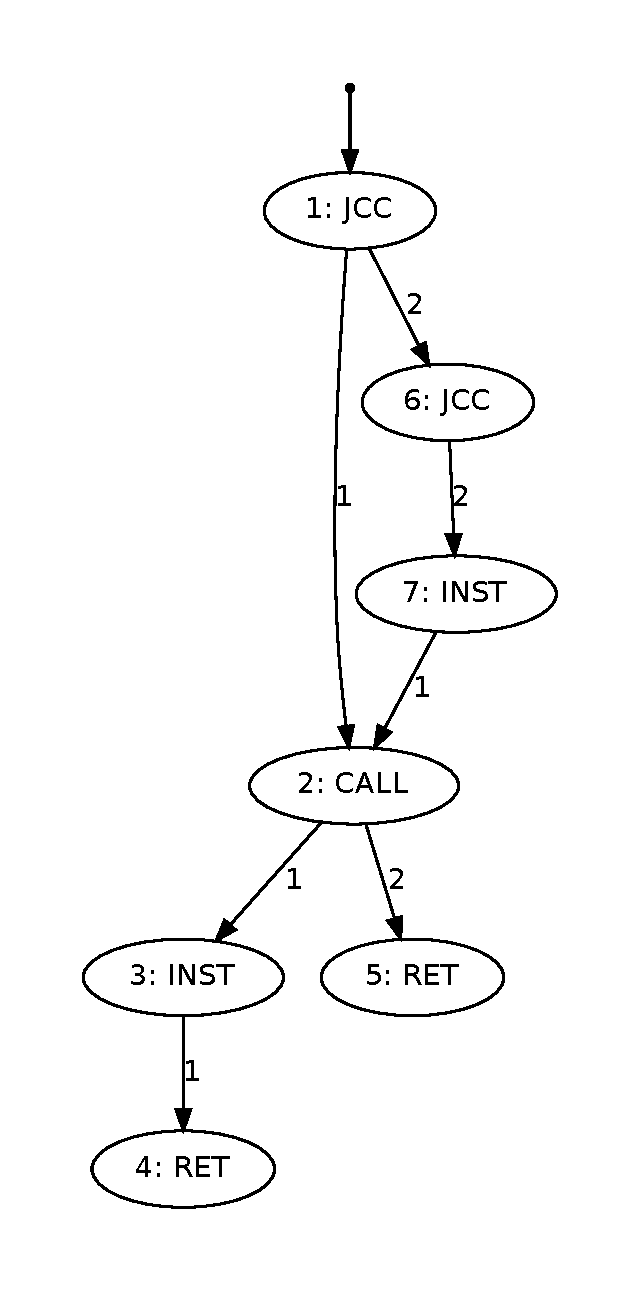
\includegraphics[height=0.4\textheight]{supports/algos/images/g1prof.pdf}
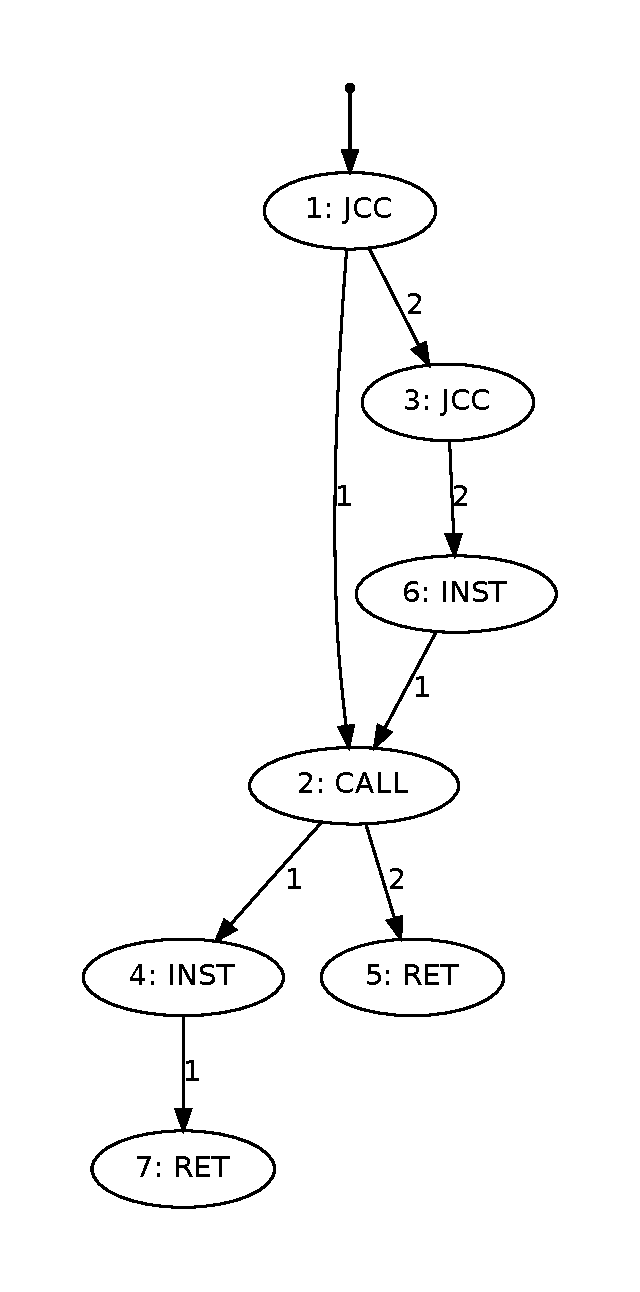
\includegraphics[height=0.4\textheight]{supports/algos/images/g1larg.pdf}
\end{center}
% \end{figure}

On peut représenter le parcours en profondeur de ce site de la manière suivante : On commence par la racine, que l'on numérote 1, c'est un JCC, puis le premier fils nous amène à un nouveau sommet, numéroté 2, c'est un CALL. Son premier fils nous amène à numéroter 3: INST et 4: RET. Une fois au $4^e$ sommet, on retourne au sommet 2 pour prendre le second fils que l'on numéroté 5: RET. On remonte au sommet 1, on numérote le second fils : c'est le sommet 6: JCC puis on prend son seul fils (fils 2) et on numéroté 7: INST. De là on prend le premier fils pour retourner sur le fils 2. Le parcours s'arrête puisqu'on a visité tous les arcs du site.\\
On peut noter le parcours ainsi (avec l'algorithme \ref{algo:codageProf}) :\\
$1: JCC\xrightarrow{1} 2: CALL \xrightarrow{1} 3: INST \xrightarrow{1} 4: RET \xrightarrow{R} 2 \xrightarrow{2} 5: RET \xrightarrow{R} 1 \xrightarrow{2} 6: JCC \xrightarrow{2} 7:INST \xrightarrow{1} 2$.\\
En fait, décrit de cette manière, le parcours définit un site unique que l'on peut reconstruire puisqu'on sait quels sont les labels de chaque sommet, tous les arcs entre les sommets et le choix des fils choisi lors du parcours (ici en profondeur).\\
De même, le parcours en largeur du site peut être décrit ainsi (avec l'algorithme \ref{algo:codageLarg}) :\\
$1: JCC\xrightarrow{1} 2: CALL\xrightarrow{R} 1\xrightarrow{2} 3: JCC\xrightarrow{R} 2\xrightarrow{1} 4: INST\xrightarrow{R} 2\xrightarrow{2} 5: RET\xrightarrow{R} 3\xrightarrow{2} 6: INST\xrightarrow{R} 4\xrightarrow{1} 7: RET$.\\
% \overset{def}



\begin{algorithm}
\caption{Codage du parcours en profondeur d'un site}
\SetAlgoLined
\KwData{Un site de racine R}
\KwResult{Le codage du parcours en profondeur de ce site}
\SetKwProg{Fn}{}{}{}
\SetKwFunction{FRecurs}{parcoursProfondeur}
\Fn(\tcc*[h]{s: sommet, i: dernier numéro attribué, E: sommets déjà explorés, etiq: associe une étiquette à un sommet, num: associe un sommet à son numéro}){\FRecurs{s, i, E, etiq, num}}{
% \Fn(// s: sommet, i: dernier numéro attribué, E: sommets déjà explorés){\FRecurs{s, i, E}}{
     \eIf{$s\notin E$}{
      $E\leftarrow E\cup\{s\}$\\
      $num(s)\leftarrow i$\\
      $C\leftarrow "i: etiq(s)"$\\
      $i\leftarrow i+1$\\
      \For{f fils numéro k de s}{
        $C\leftarrow C+"\xrightarrow{k}"$\\
	$(i, c)\leftarrow parcoursProfondeur(f, i, E, etiq, num)$\\
	$C\leftarrow C+ c$\\
	\If{s a encore au moins un fils}{
	$C\leftarrow C+ "\xrightarrow{R} num(s)"$\\
	}
      }
      	$retourner (i, C)$\\
     }
     {
     $retourner (i, "num(s)")$\\
     }
}
parcoursProfondeur(R, 1, $\emptyset$, etiq, $\emptyset$)
\label{algo:codageProf}
\end{algorithm}

\begin{algorithm}
\caption{Codage du parcours en largeur d'un site}
\SetAlgoLined
\KwData{Un site de racine R}
\KwResult{Le codage du parcours en largeur de ce site}
\SetKwProg{Fn}{}{}{}
\SetKwFunction{FRecurs}{parcoursLargeur}
\Fn(\tcc*[h]{etiq: associe une étiquette à un sommet}){\FRecurs{etiq}}{
% \Fn(// s: sommet, i: dernier numéro attribué, E: sommets déjà explorés){\FRecurs{s, i, E}}{

}
$s_c\leftarrow \epsilon$\tcc*[H]{Le sommet courant devient $\epsilon$.}
% $num(R)\leftarrow 1$\tcc*[H]{Il est numéroté 1.}
$i\leftarrow 1$\tcc*[H]{On numérote à partir de 1.}
$C\leftarrow ""$\\
$A\leftarrow [(\epsilon, 0, R)]$\tcc*[H]{A contient les sommets à visiter.}
$E\leftarrow \{\}$\tcc*[H]{E est l'ensemble des sommets déjà visités.}
\While{il y a un premier élément a=(p, k, s) dans A}{
  Retirer le premier élément de A\\
  \If{$s_c$ n'est ni p ni $\epsilon$}
  {
    $C\leftarrow C+ "\xrightarrow{R} num(p)"$\\
    $s_c\leftarrow p$
  }
  \eIf{s n'est pas dans E}
  {
    \eIf{p est $\epsilon$}{
      $C\leftarrow C+ "1: etiq(R)"$\\
    }
    {
      $C\leftarrow C+ "\xrightarrow{k} i: etiq(s)"$\\
    }
    $num(s)\leftarrow i$\\
    $i\leftarrow i+1$\\
    $s_c\leftarrow s$\\
    \For{fils f numéro k' du sommet s}
    {  
      $A\leftarrow A + (s, k', f)$
    }
    $E\leftarrow E\cup \{s\}$\\
  }
  {
    $C\leftarrow C+ "\xrightarrow{k} num(s)"$\\
    $s_c\leftarrow s$\\
  }
}
\Return C
\label{algo:codageLarg}
\end{algorithm}


On peut reconstuire le site à partir du codage précédent en procédant de manière incrémentale (algorithme \ref{algo:siteDepuisCodage}) si le codage est bien formé (définition \ref{def-codage-bien-forme}).
Par la suite on ne parlera que de codages bien formés sans l'expliciter.
\begin{defi}
\label{def-codage-bien-forme}
 Un codage de parcours est bien formé s'il vérifie :
\begin{enumerate}
 \item Il est de la forme $1:L(\xrightarrow{\alpha}i[:L])*$ avec L une étiquette et $\alpha$ un entier k ou R
 \item L'étiquette de chaque sommet est spécifiée une unique fois : lors la première référence à ce sommet
%  \item S'il y a deux mots de la forme $i:L_1$ et $i:L_2$ alors $L_1=L_2$
 \item Pour tout mot de la forme $\xrightarrow{R}i[:L]$, un mot $i:L$ est présent précédemment dans le codage
 \item Il ne définit qu'une fois chaque fils de chaque sommet : à $i$ et $k$ fixés, il ne doit y avoir qu'une seule occurence de $i[:L]\xrightarrow{k}$
%  \item Toute suite incluse dans le codage de la forme $1:L(\xrightarrow{\alpha}i[:L])*$ est également un parcours
\end{enumerate} 
\end{defi}



\begin{algorithm}[H] %or another one check
\caption{Reconstruction d'un site depuis son codage}
\SetAlgoLined
\KwData{Le codage d'un site}
\KwResult{Un site}
\SetKwProg{Fn}{}{}{}
\SetKwFunction{FRecurs}{reconstructionSite}
\Fn(\tcc*[h]{Le codage est de la forme $1:L(\xrightarrow{\alpha}i[:L])*$}){\FRecurs{codage}}{
% \Fn(// s: sommet, i: dernier numéro attribué, E: sommets déjà explorés){\FRecurs{s, i, E}}{
Création d'un site vide\\
Ajout du sommet 1 d'étiquette L qui est la racine du site et devient le sommet courant\\
  \For{chaque suite de symboles de type $\xrightarrow{\alpha}i[:L]$}{
  \eIf{$\alpha$ est un entier k}{
  Ajout du sommet i d'étiquette L s'il n'existait pas\\
  Ajout d'un arc entre le sommet courant et le sommet i\\
  Le sommet i devient le sommet courant
  }
  {
  Le sommet i devient le sommet courant
  }
  }
}
\label{algo:siteDepuisCodage}
\end{algorithm}
% \begin{prop}
% Soit $S_1$ et $S_2$ deux sites dont les codages de parcours en profondeur (générés par l'algorithme \ref{algo:codageProf}) sont $C_1$ et $C_2$.\\
% $C_1=C_2\Rightarrow S_1$ et $S_2$ sont deux sites isomorphes.
% \end{prop}
% 
% \begin{pr}
%  On a supposé que l'algorithme \ref{algo:siteDepuisCodage} inverse l'algorithme \ref{algo:codageProf} pour des codages bien formés.
% \end{pr}
% 
% \begin{prop}
% \label{prop:isoCodage}
% Soit $C_1$ et $C_2$ deux codages de parcours dont les sites résultants (par l'algorithme \ref{algo:siteDepuisCodage}) sont $S_1$ et $S_2$.\\
% $S_1$ et $S_2$ sont deux sites isomorphes $\Rightarrow C_1=C_2$.\\
% (c'est faux)
% \end{prop}
% 
L'algorithme \ref{algo:parcoursSiteDepuisCodage} tente de trouver le sous-site désigné par un codage dans un graphe de flot T, à partir d'un sommet donné. S'il ne renvoie pas FAIL, il fournit un site qui est effectivement un sous-site du graphe (les sommets et les arcs sont forcément dans T, et ils sont accessibles à partir de la racine vu qu'il s'agit d'un parcours).

\begin{algorithm}[H] %or another one check
\caption{Reconstruction d'un sous-site de graphe de flot à partir d'un sommet donné, depuis son codage}
\SetAlgoLined
\KwData{Le codage d'un site, un graphe de flot T, un sommet R de T}
\KwResult{Un site ou FAIL}
\SetKwProg{Fn}{}{}{}
\SetKwFunction{FRecurs}{reconstructionSousSite}
\Fn(\tcp*[h]{Le codage est de la forme $1:L(\xrightarrow{\alpha}i[:L])*$}){\FRecurs{codage, T, R}}{
\eIf{le sommet R a l'étiquette L}{
  On numérote R par 1.\\
  Le sommet numéroté 1 devient le sommet courant.
}
{
  \Return FAIL
}
  \For{chaque suite de symboles de type $\xrightarrow{\alpha}i[:L]$}{
  \eIf{$\alpha$ est un entier k}{
  \uIf{le sommet courant a un fils k non numéroté, d'étiquette L, et aucun sommet n'est numéroté i}{
  On numérote ce fils k par i.\\
  Le sommet numéroté i devient le sommet courant.
  }
  \uElseIf{le sommet courant a un fils k numéroté i}{
  Le sommet numéroté i devient le sommet courant.
  }
  \Else{
  \tcp{Le parcours n'est pas possible si :\\ un autre sommet est déjà numéroté i,  ou\\ si le sommet à numéroter a déjà une autre numérotation,  ou\\ si l'étiquette n'est pas la bonne, ou\\ s'il n'y a pas de fils k}
  \Return FAIL
  }
  }
  {
  Le sommet i devient le sommet courant
  }
  }
  \Return le site constitué des sommets numérotés et des arcs empruntés.
}
\label{algo:parcoursSiteDepuisCodage}
\end{algorithm}

On voudrait maintenant prouver l'équivalence entre l'existence d'un isomorphisme de sous-site entre un site P et un graphe de flot T d'une part, et la possibilité d'appliquer un parcours bien formé quelconque de P à partir d'un sommet de T. Les deux propositions suivantes vont permettre d'établir l'équivalence statuée au théorème \ref{theo:eqIsoCodage}.

\begin{prop}
 Soit un codage C d'un parcours, $S_C$ son site associé par l'algorithme \ref{algo:siteDepuisCodage}, T un graphe de flot et R un sommet de T.\\
 Si un parcours de T à partir de R renvoie un site S (algorithme \ref{algo:parcoursSiteDepuisCodage}), alors $S_C$ et S sont isomorphes.
 \label{prop:condageDoncIso}
\end{prop}

\begin{pr}
 Les sous-sites restreints à leur racine sont isomorphes (un seul sommet avec la même étiquette), numérotés de la même manière et le sommet courant est le même.\\
 Supposons que les sous sites restreints aux sommets du parcours $1:L_1\xrightarrow{\alpha_1}i_2[:L_2]\xrightarrow{\alpha_2} ...\xrightarrow{\alpha_{p-1}}i_{p}[:L_{p}]$ sont isomorphes.\\
 Lors de l'étape suivante du parcours ($\xrightarrow{\alpha}i[:L]$), le seul cas où un sommet est numéroté est si $\alpha$ est un entier $k$, si le sommet courant dans T a un fils k non numéroté d'étiquette L et aucun sommet n'est déjà numéroté i. Dans cas un sommet est ajouté au site créé par l'algorithme \ref{algo:siteDepuisCodage} à partir du sommet courant. Dans les deux cas la numérotation est la même et le sommet courant est le sommet qui vient d'être numéroté ou ajouté.\\
 Le second cas possible est si le sommet courant a un fils k déjà numéroté i et d'étiquette L. Dans ce cas ce sommet a déjà été ajouté au sité créé par l'algorithme \ref{algo:siteDepuisCodage}, il n'y a ni numérotation ni ajout de site et le sommet courant devient le fils k.\\
  Les arcs sont nécessairement les mêmes puisque les parcours appliqués dans les deux algorithmes sont identiques. \\
 Tous les autres cas provoquent un arrêt du parcours par un FAIL. \\
 On a bien montré que dans les cas ne provoquant pas d'erreur, les deux sites restreints aux sommets du parcours sont isomorphes.
\end{pr}

\begin{prop}
 Si P est un site isomorphe à un sous-site S d'un graphe de flot T alors tout codage de parcours $C_P$ de P peut être parcouru dans T à partir de la racine de S.
 \label{prop:isoDoncCodage}
\end{prop}

\begin{pr}
On va montrer que l'algorithme \ref{algo:parcoursSiteDepuisCodage} appliqué au codage $C_P$, au graphe T, à partir de la racine de S produit un site S' isomorphe à S et P. \\
Le graphe composé uniquement de la racine de P est isomorphe à celui composé de la racine de S ajoutée au graphe à construire dans l'algorithme \ref{algo:parcoursSiteDepuisCodage}. \\
Supposons que les sous sites restreints aux sommets du parcours $1:L_1\xrightarrow{\alpha_1}i_2[:L_2]\xrightarrow{\alpha_2} ...\xrightarrow{\alpha_{p-1}}i_{p}[:L_{p}]$ sont isomorphes et que les numérotations correspondent à l'isomorphisme.\\
Lors de l'étape suivante du parcours ($\xrightarrow{\alpha}i[:L]$), un sommet n'est ajouté dans l'algorithme \ref{algo:siteDepuisCodage} que si $\alpha$ est un entier $k$ et si le sommet $i$ n'a pas déjà été créé. Dans le parcours de T (algorithme \ref{algo:parcoursSiteDepuisCodage}), cela implique qu'aucun sommet n'est déjà numéroté $i$. Puisque le sommet courant dans P a un fils $k$, que les sommets courants de P et S' sont correspondant dans l'isomorphisme et que P et S sont isomorphes, le sommet courant dans S' a un fils $k$ (d'étiquette $L$). Puisque le codage est bien formé, il n'y a qu'un fils $k$ du sommet courant. Ce fils $k$ n'a pas déjà été numéroté, sinon il aurait déjà été créé précédemment dans l'algorithme \ref{algo:siteDepuisCodage}. On est donc nécessairement dans le cas où on numérote le fils $k$ du sommet courant par i, le sommet ajouté dans l'algorithme \ref{algo:siteDepuisCodage} porte le même numéro que celui numéroté dans le parcours de T : ils se correspondent dans un isomorphisme de 
sites.\\
Dans le cas contraire où aucun fils n'est ajouté, comme précédemment le sommet courant a nécessairement un fils $k$ qui a déjà été numéroté puisque c'est le cas dans la reconstruction du site P. Dans les deux cas aucun site n'est ajouté mais le fils $k$ devient le sommet courant.\\
On en déduit que les sommets ajoutés sont toujours deux sommets correspondants dans un isomorphisme et que les arcs ajoutés sont également les mêmes.
\end{pr}

\begin{theo}
 Soit P un site et T un graphe de flot. Les deux propositions suivantes sont équivalents :
 \begin{itemize}
  \item P est isomorphe à un sous-site de T
  \item Il existe C un codage de parcours bien formé de P tel que le parcours de C est possible dans T
 \end{itemize}
\label{theo:eqIsoCodage}
\end{theo}

\begin{pr}
~
 \begin{itemize}
 \renewcommand{\labelitemi}{$\bullet$}
  \item Si P est isomorphe à un sous-site de T, on peut appliquer la proposition \ref{prop:isoDoncCodage} au parcours en profondeur, ce qui donne directement le résultat.
  \item S'il existe un codage C de parcours de P que l'on peut également parcourir dans T, alors on construit son site associé avec l'algorithme \ref{algo:siteDepuisCodage} et on applique la proposition \ref{prop:condageDoncIso} qui donne le résultat.
 \end{itemize}
\end{pr}

L'intérêt de cet équivalence est qu'elle donne un algorithme simple et bien plus efficace que celui d'Ullmann pour résoudre le problème \ref{pbisosg} d'isomorphisme de sous-site entre un site de motif et un graphe de flot de test.

\subsection{Application directe}
\subsubsection{Résolution des problèmes d'isomorphisme}
L'équivalence entre isomorphisme et parcours permet de résoudre le problème \ref{pbisog} de la manière suivante :
Deux sites sont isomorphes si et seulement si leurs codages de parcours en profondeur\footnote{On peut substituer le parcours en profondeur par un parcours en largeur on n'importe quel codage de parcours bien formé} sont identiques.

Le problème \ref{pbisosg} de l'existence d'un isomorphisme entre un site et un sous-site d'un site peut être résolu ainsi :
Il existe un sous-site de T isomorphe au site P si et seulement si il existe un sommet de T à partir duquel le codage du parcours en profondeur\footnotemark[\value{footnote}] de P est possible.

Une solution au problème \ref{pbisosgbase} de l'existence d'un site dans une base $L_S$ isomorphe à un sous-site d'un site T consiste à itérer la solution précédente de l'isomorphisme de sous-site à chaque site de la base $L_S$.

\subsubsection{Complexité}
La résolution du problème de l'isomorphisme de sous-site avec cet algorithme se réalise dans le pire des cas en $O(n_T.n_P)$ puisqu'elle nécessite :
\begin{itemize}
 \item Un parcours en profondeur du site de motif P avec détermination du codage : $O(n_P)$
 \item Un parcours du graphe de flot T à partir de chacun de ses sommets : chaque parcours se fait en $O(n_P)$, cette étape peut alors se réaliser en $O(n_T.n_P)$
\end{itemize}
~\\

Si on a une base de $n$ sites $L_S$ de taille $W$, la complexité dans le pire des cas pour déterminer un site de la base est isomorphe à un sous-site de T est $O(n.n_T.W)$.


\subsection{Codages rangés dans un arbre de décision}
\subsubsection{Création d'un arbre de décision des codages}
On peut générer les codages de parcours en profondeur de chaque site de la base puis les ranger dans un arbre de décision. Par exemple trois sites donnés en figure \ref{fig:troisProf}, dont les parcours en profondeur sont (dans l'ordre):\\
$1: JCC\xrightarrow{1} 2: CALL \xrightarrow{1} 3: INST \xrightarrow{1} 4: RET \xrightarrow{R} 2 \xrightarrow{2} 5: RET \xrightarrow{R} 1 \xrightarrow{2} 6: JCC \xrightarrow{2} 7:INST \xrightarrow{1} 2$
\\
$1: JCC\xrightarrow{1} 2: CALL \xrightarrow{1} 3: INST \xrightarrow{1} 4: RET \xrightarrow{R} 2 \xrightarrow{2} 5: RET \xrightarrow{R} 1 \xrightarrow{2} 6: JCC \xrightarrow{2} 7:INST \xrightarrow{1} 3$
\\
$1: JCC\xrightarrow{1} 2: RET \xrightarrow{R} 1 \xrightarrow{2} 3: JCC \xrightarrow{2} 4: INST \xrightarrow{1} 5: CALL \xrightarrow{1} 6: INST \xrightarrow{1} 2 \xrightarrow{R} 5 \xrightarrow{2} 7: RET$

L'arbre de décision créé à partir de ces trois codages est donné en figure \ref{fig:arbreDecTarjan}. L'ajout d'un codage à l'arbre de décision est standard et ne sera pas détaillée.

\begin{figure}
\begin{center}
\subfigure[]{
\label{fig:troisProf1}
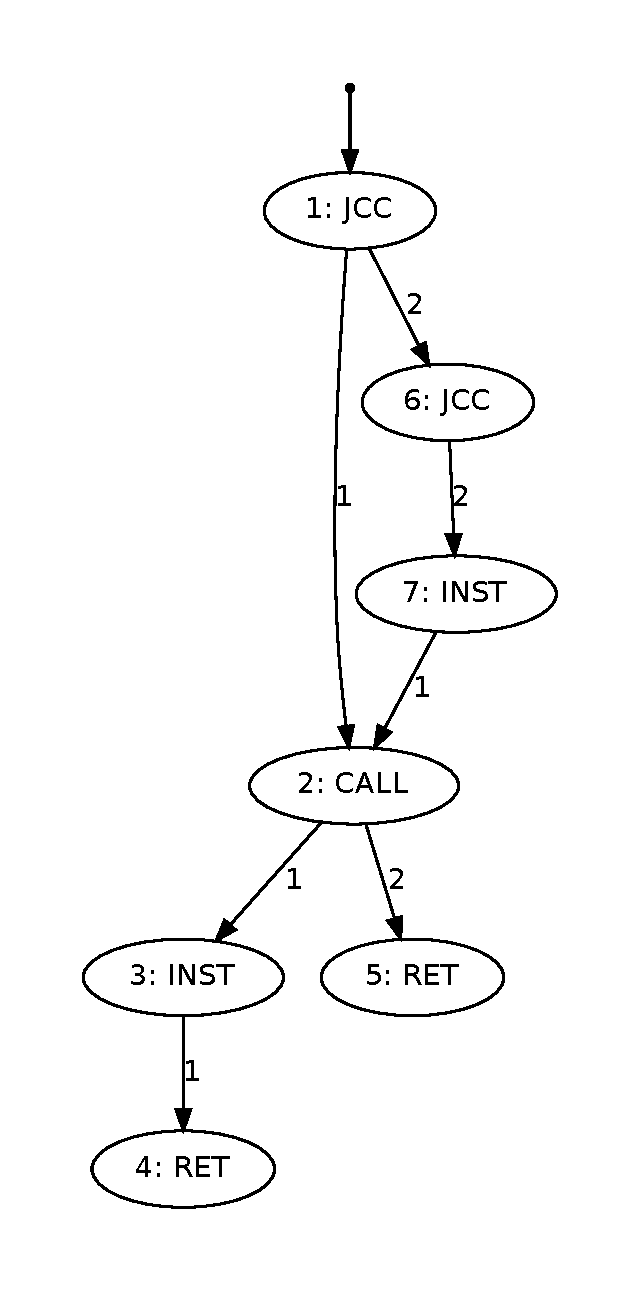
\includegraphics[height=0.4\textheight]{supports/algos/images/g1prof.pdf}}
\subfigure[]{
\label{fig:troisProf2}
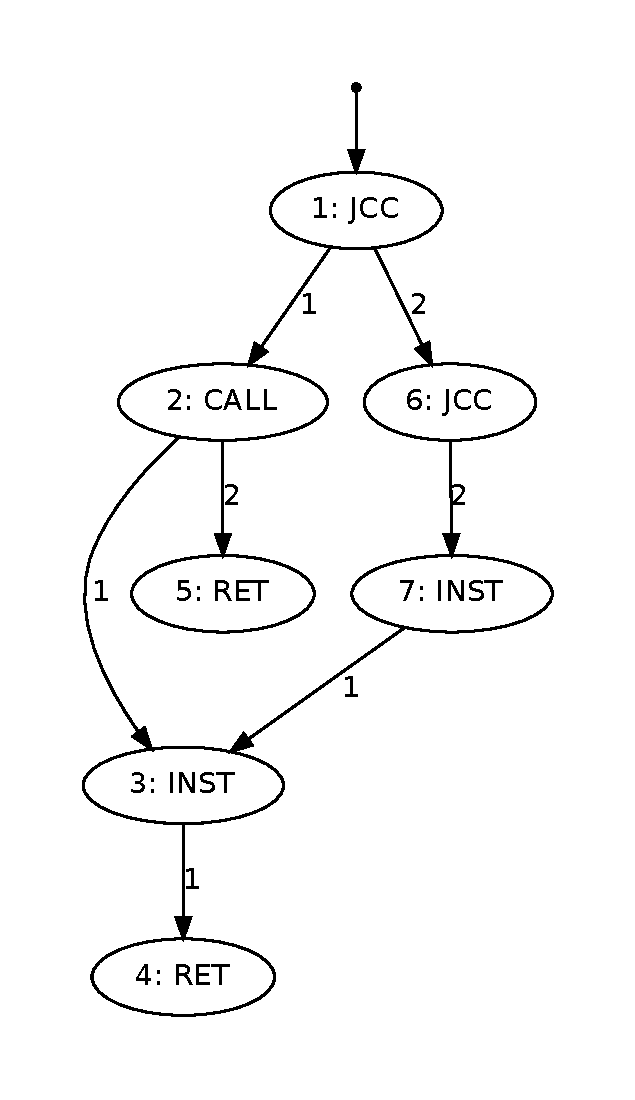
\includegraphics[height=0.4\textheight]{supports/algos/images/g2prof.pdf}}
\subfigure[]{
\label{fig:troisProf3}
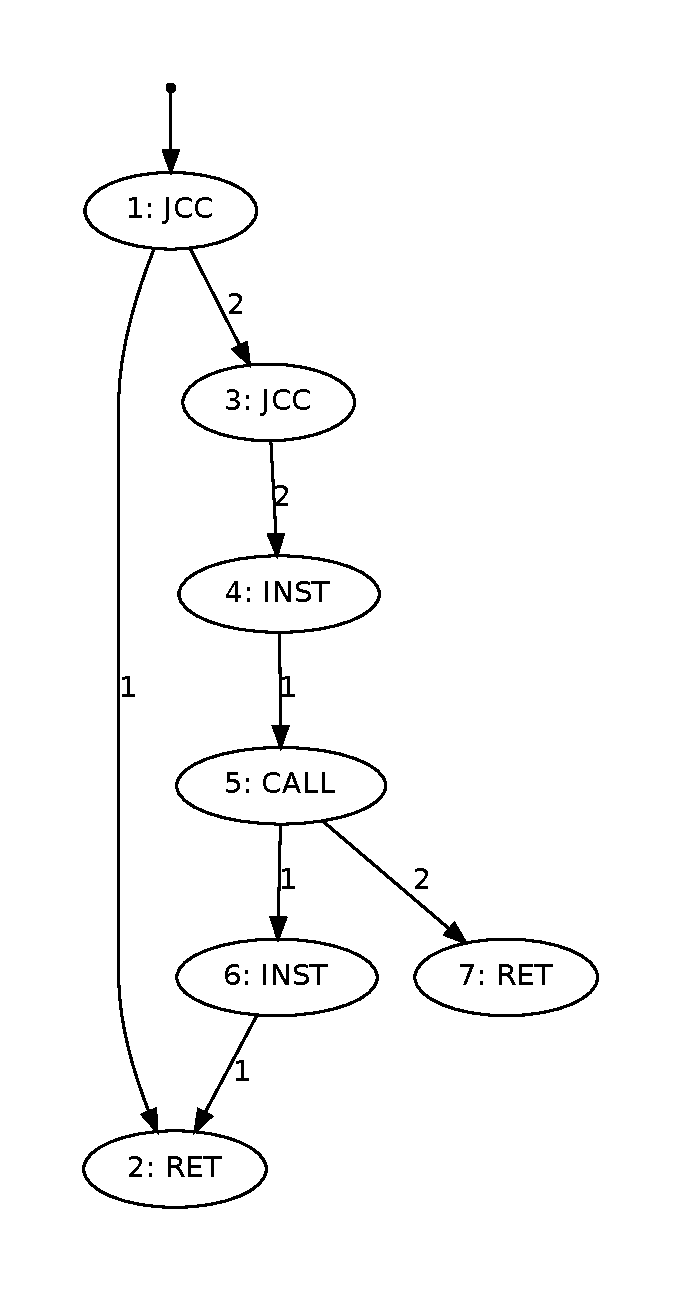
\includegraphics[height=0.4\textheight]{supports/algos/images/g3prof.pdf}}
\end{center}
\caption{Trois sites numérotés selon un parcours en profondeur}
\label{fig:troisProf}
\end{figure}
% $1: JCC\xrightarrow{1} 2: CALL \xrightarrow{1} 3: INST \xrightarrow{1} 4: RET \xrightarrow{R} 2 \xrightarrow{2} 5: RET \xrightarrow{R} 1 \xrightarrow{2} 6: JCC \xrightarrow{2} 7:INST \xrightarrow{1} 2$

\begin{figure}
\begin{center}
\begin{tikzpicture}[
  tlabel/.style={pos=0.4,right=-1pt,font=\footnotesize\color{black!70!black} },
  every node/.style={color=black!25!black, circle, minimum size=6mm, draw=black!75, align=center},
  edge from parent/.style={draw=black!50,thick},
  level 1/.style={sibling distance=50mm, level distance=12mm},
]
\node[rectangle, rounded corners]{$racine$}
child {node {}
       child{node {}
	     child {node {}
	            child {node {}
		           child {node {}
		                  child {node {}
		                         child {node {}
		                                child {node {}
		                                       child {node {}
		                                              child {node {a}
								edge from parent node[tlabel,pos=0.2, left=15pt,draw=none] {$\xrightarrow{1} 2$}
		                                              }
		                                              child {node {b}
								edge from parent node[tlabel,pos=0.2, right=11pt,draw=none] {$\xrightarrow{1} 3$}
		                                              }
		                                              edge from parent node[tlabel,pos=0.3,draw=none] {$\xrightarrow{2} 7:INST$}
		                                       }
		                                       edge from parent node[tlabel,pos=0.3,draw=none] {$\xrightarrow{2} 6: JCC$}
		                                }
		                                edge from parent node[tlabel,pos=0.3,draw=none] {$\xrightarrow{R} 1$}
		                         }
		                         edge from parent node[tlabel,pos=0.3,draw=none] {$\xrightarrow{2} 5: RET$}
		                  }
		                  edge from parent node[tlabel,pos=0.3,draw=none] {$\xrightarrow{R} 2$}
		           }
		           edge from parent node[tlabel,pos=0.3,draw=none] {$\xrightarrow{1} 4: RET$}
	            }
	            edge from parent node[tlabel,pos=0.3,draw=none] {$\xrightarrow{1} 3: INST$}
	     }
	     edge from parent node[tlabel,pos=0.1, left=15pt,draw=none] {$\xrightarrow{1} 2: CALL$}
       }
       child{node {}
	     child {node {}
	            child {node {}
		           child {node {}
		                  child {node {}
		                         child {node {}
		                                child {node {}
		                                       child {node {}
		                                              child {node {c}
		                                              edge from parent node[tlabel,pos=0.3,draw=none] {$\xrightarrow{2} 7: RET$}
		                                              }
		                                              edge from parent node[tlabel,pos=0.3,draw=none] {$\xrightarrow{R} 5$}
		                                       }
		                                       edge from parent node[tlabel,pos=0.3,draw=none] {$\xrightarrow{1} 2$}
		                                }
		                                edge from parent node[tlabel,pos=0.3,draw=none] {$\xrightarrow{1} 6: INST$}
		                         }
		                         edge from parent node[tlabel,pos=0.3,draw=none] {$\xrightarrow{1} 5: CALL$}
		                  }
		                  edge from parent node[tlabel,pos=0.3,draw=none] {$\xrightarrow{2} 4: INST$}
		           }
		           edge from parent node[tlabel,pos=0.3,draw=none] {$\xrightarrow{2} 3: JCC$}
	            }
	            edge from parent node[tlabel,pos=0.3,draw=none] {$\xrightarrow{R} 1$}
	     }
	     edge from parent node[tlabel,pos=0.1, right=5pt,draw=none] {$~~~\xrightarrow{1} 2: RET$}
       }
       edge from parent node[tlabel,pos=0.5,draw=none] {$1: JCC$}
};
\end{tikzpicture}
\end{center}
\caption{Arbre de décision contenant les codages de sites de la figure \ref{fig:troisProf}}
\label{fig:arbreDecTarjan}
\end{figure}

\paragraph{Complexité.}
L'ajout d'un site à la base consiste à ajouter un codage de parcours dans l'arbre de décision, cette opération nécessite un nombre de comparaison en $W.i$ où $i$ est le nombre de fils maximum de chaque sommet de l'arbre. Vue que les étiquettes des arcs de l'arbre sont de la forme $[\xrightarrow{\alpha}]i[:L]$, en notant $K$ le nombre de fils maximum de chaque sommet dans un site et $n_L$ le nombre d'étiquettes différentes pour les sommets des sites, $i\leq (K+2).W.n_L$ soit $n=O(W)$ donc l'ajout d'un site à la base se fait en $O(W^2)$.

\subsubsection{Recherche d'un isomorphisme de sous-sites à partir de l'arbre de décision}
Une fois l'arbre généré à partir de tous les codages des sites de $L_S$, on veut l'utiliser pour trouver tous les parcours de $L_S$ possibles dans le graphe de flot T. Pour compter le nombre de parcours de l'arbre que l'on peut réaliser à partir du sommet $r$ de $T$, on peut chercher à parcourir $T$ à partir de $r$ en parcourant les branches possibles dans l'arbre de décision. À chaque fois qu'on peut parcourir une branche jusqu'en bas c'est qu'un site isomorphe a été trouvé. L'algorithme \ref{algo:rechercheArbreTarjan} compte le nombre de ces branches possibles.

On peut utiliser cet algorithme pour retrouver tous les sous-sites isomorphes en utilisant l'algorithme précédent à partir de chaque sommet de $T$.

\begin{figure}
\begin{algorithm}[H] %or another one check
\caption{Décompte des parcours d'un arbre de parcours possibles dans un graphe de flot, à partir d'un sommet donné}
\SetAlgoLined
\KwData{Un arbre A contenant les parcours de sites, un graphe de flot T, un sommet r de T}
\KwResult{Le nombre de parcours possibles}
\SetKwProg{Fn}{}{}{}
\SetKwFunction{FRecurs}{decompteSousSite}
\Return decompteSousSite(A, racine(A), T, r)\\
~\\

\Fn{\FRecurs{A, a, T, R}}{
  \eIf{a n'a aucun fils dans A}{
    \tcp{Si a n'a aucun fils, on a exactement décrit un parcours}
    \Return 1
  }
  {
    $somme\leftarrow 0$\\
    \For{f fils d'étiquette e de a dans A}{
	$(possible, s', T') \leftarrow etape(e, s, T)$\\
	\If{possible}{
	  $somme\leftarrow somme+decompteSousSite(A, f, T', s')$
	}
    }
  }
}

\SetKwProg{Fn}{}{}{}
\SetKwFunction{FRecurs}{etape}
\Fn(\tcp*[h]{L'étiquette e est de la forme $[\xrightarrow{\alpha}]i[:L]$}){\FRecurs{e, s, T}}{
  \eIf{e est de la forme $1:L$}{
    Numéroter le sommet s de T par 1.\\
    \Return (true, s, T)
  }
  {
    \tcp{Dans ce cas e est de la forme $\xrightarrow{\alpha}i[:L]$}
    \eIf{$\alpha$ est un entier k}{
    \uIf{s a un fils s' d'ordre k non numéroté dans T, d'étiquette L, et aucun sommet n'est numéroté i}{
    On numérote s' par i dans T.\\
    \Return $(true, s', T)$
    }
    \uElseIf{le sommet courant a un fils s' d'ordre k numéroté i}{
    \Return $(true, s', T)$
    }
    \Else{
    \tcp{Le parcours n'est pas possible si :\\ un autre sommet est déjà numéroté i,  ou\\ si le sommet à numéroter a déjà une autre numérotation,  ou\\ si l'étiquette n'est pas la bonne, ou\\ s'il n'y a pas de fils k}
    \Return $(false, s ,T)$
    }
    }
    {
      \tcp{Dans ce cas e est de la forme $\xrightarrow{R}i$}
      On note s' le sommet numéroté i dans T.\\
      \Return $(true, s', T)$
    }
  }
}
\label{algo:rechercheArbreTarjan}
\end{algorithm}
\end{figure}

\paragraph{Complexité.}
Dans le pire des cas il y a $n$ branches à l'arbre A qui partent de la racine où $n$ est le nombre de sites dans la base. Le parcours d'une branche avec au maximum un fils à chaque sommet, à partir de la racine se fait en $O(W)$ au vu de la récursion de l'algorithme  \ref{algo:rechercheArbreTarjan}. Pour chercher les isomorphismes de sous-sites de $T$ il faut répéter l'opération pour chacun de ses sommets : la complexité totale dans le pire des cas pour résoudre le problème \ref{pbisosgbase} d'isomorphisme de sous-sites entre un graphe de flot et une base de sites est de $O(n.n_T.W)$. Ainsi on n'a pas amélioré la complexité dans le pire des cas par rapport à l'utilisation directe du parcours de Tarjan vu dans la section précédente, bien qu'en pratique l'algorithme soit plus rapide comme nous le verrons par la suite.

\clearpage
\section{SIDT : Site Isomorphism Decision Tree}
Le problème \ref{pbisosg} consiste à détecter un site P dans un graphe de flot T. En pratique le site P aura été généré à partir d'un graphe de flot G. Si P est un sous-site de T, puisqu'on a généré le site à partir d'un parcours dans un autre graphe de flot, on peut envisager que le même parcours appliqué à T est susceptible de générer le site P. Ce n'est pas vrai dans le cas général et en ce sens l'algorithme présenté ici n'est pas complet.\\
Inversement il est clair que si le même parcours appliqué à partir de sommets de T et G génèrent le même site P, alors P est bien un sous-site de T.
\\

On se propose donc, pour approcher la solution au problème \ref{pbisosg} de détection d'isomorphisme de sous-site entre un site P (généré par parcours avec un algorithme A à partir d'un sommet d'un graphe de flot G) et un graphe de flot T, de générer tous les sous-sites de T avec l'algorithme de parcours A et de regarder si P est dans cet ensemble.

Pour régler le problème \ref{pbisosgbase} de détection d'un site dans une base de graphes de flot, on va créer un arbre de décision contenant tous les sites générés à partir du parcours par A des graphes de flot de la base.

\subsection{Arbre de décision pour la détection de sites}
Chaque site est généré par un parcours numérotant ses sommets, et chaque sommet a un nombre de fils bornés. On représente alors les sites sous forme matricielle : chaque ligne représente un sommet, le premier élément de la colonne est l'étiquette du sommet et les éléments suivants sont les numéros des fils de ce sommet (0 indique qu'il n'y a pas de sommet). La représentation des sites de la figure \ref{fig:troisProf} est donnée figure \ref{fig:troisProfMatRed}.
On peut ensuite agréger tous les sites générés dans un arbre de décision (figure \ref{fig:arbreDecTarjan}).

\begin{figure}
\begin{center}
\subfigure[]{
\label{fig:troisProfMatRed1}
$\begin{array}{r|ccc} Sommet & Etiquette & Fils 1 & Fils 2 \\
\hline
1 & JCC & 2 & 6\\
2 & CALL & 3 & 5\\
3 & INST & 4 & 0\\ 
4 & RET & 0 & 0\\ 
5 & RET & 0 & 0\\ 
6 & JCC & 0 & 7\\ 
7 & INST & 2 & 0\\ 
\end{array}$
}
\subfigure[]{
\label{fig:troisProfMatRed2}
$\begin{array}{r|ccc} Sommet & Etiquette & Fils 1 & Fils 2 \\
\hline
1 & JCC & 2 & 6\\
2 & CALL & 3 & 5\\
3 & INST & 4 & 0\\ 
4 & RET & 0 & 0\\ 
5 & RET & 0 & 0\\ 
6 & JCC & 0 & 7\\ 
7 & INST & 3 & 0\\ 
\end{array}$
}
\subfigure[]{
\label{fig:troisProfMatRed3}
$\begin{array}{r|ccc} Sommet & Etiquette & Fils 1 & Fils 2 \\
\hline
1 & JCC & 2 & 3\\
2 & RET & 0 & 0\\
3 & JCC & 0 & 4\\ 
4 & INST & 5 & 0\\ 
5 & CALL & 6 & 7\\ 
6 & INST & 2 & 0\\ 
7 & RET & 0 & 0\\ 
\end{array}$
}
\end{center}
\caption{Représentation matricielle des sites de la figure \ref{fig:troisProf}}
\label{fig:troisProfMatRed}
\end{figure}

\begin{figure}
\begin{center}
\begin{tikzpicture}[
  tlabel/.style={pos=0.4,right=-1pt,font=\footnotesize\color{black!70!black} },
  every node/.style={color=black!25!black, circle, minimum size=6mm, draw=black!75, align=center},
  edge from parent/.style={draw=black!50,thick},
  level 1/.style={sibling distance=50mm, level distance=12mm},
]
\node[rectangle, rounded corners]{$racine$}
child{node{}
      child{node {}
	     child {node {}
	            child {node {}
		           child {node {}
		                  child {node {}
		                         child {node {a}
		                                edge from parent node[tlabel,pos=0.2, left=10pt,draw=none] {INST 2 0}
		                         }
		                         child {node {b}
		                                edge from parent node[tlabel,pos=0.2, right=12pt,draw=none] {INST 3 0}
		                         }
		                         edge from parent node[tlabel,pos=0.3,draw=none] {JCC 0 7}
		                  }
		                  edge from parent node[tlabel,pos=0.3,draw=none] {RET 0 0}
		           }
		           edge from parent node[tlabel,pos=0.3,draw=none] {RET 0 0}
	            }
	            edge from parent node[tlabel,pos=0.3,draw=none] {INST 4 0}
	     }
	     edge from parent node[tlabel,pos=0.1, right=5pt,draw=none] {CALL 3 5}
       }
       edge from parent node[tlabel,pos=0.3,left=10pt,draw=none] {JCC 2 6}
      }
child {node {}
       child{node {}
	     child {node {}
	            child {node {}
		           child {node {}
		                  child {node {}
		                         child {node {c}
		                                edge from parent node[tlabel,pos=0.3,draw=none] {RET 0 0}
		                         }
		                         edge from parent node[tlabel,pos=0.3,draw=none] {INST 2 0}
		                  }
		                  edge from parent node[tlabel,pos=0.3,draw=none] {CALL 6 7}
		           }
		           edge from parent node[tlabel,pos=0.3,draw=none] {INST 5 0}
	            }
	            edge from parent node[tlabel,pos=0.3,draw=none] {JCC 0 4}
	     }
	     edge from parent node[tlabel,pos=0.1, right=5pt,draw=none] {RET 0 0}
       }
       edge from parent node[tlabel,pos=0.3,right=12pt,draw=none] {JCC 2 3}
};
\end{tikzpicture}
\end{center}
\caption{Arbre de décision contenant les matrices de la figure \ref{fig:troisProfMatRed}}
\label{fig:arbreDecSIDT}
\end{figure}

\paragraph{Complexité.}
L'apprentissage d'un site nécessite le parcours d'au plus W éléments de l'arbre de décision. Chaque sommet de l'arbre de décision a au plus $n_L.W.W$ fils où $n_L$ est le nombre d'étiquettes possibles. L'apprentissage d'un site se fait donc en $O(W^3)$ où W est le nombre de sommets des sites à apprendre.

\subsection{Recherche d'un isomorphismes de sous-sites}
Rechercher un isomorphisme de sous-sites à partir de l'arbre de décision ainsi créé revient à écrire le site sous forme matricielle et à faire une recherche dans l'arbre de décision.

\paragraph{Complexité.}
La complexité de la recherche d'un site dans l'arbre de décision est la même que pour l'ajout dans d'un site dans l'arbre et se fait en $O(W^3)$. 


\section{Comparaisons des performances}
On a donc trois algorithmes à comparer : l'algorithme d'Ullmann, pris pour référence, l'algorithme de Tarjan avec arbre de décision et l'algorithme incomplet par arbre de décision (SIDT).

\begin{center}
\begin{tabular}{|c|c|c|}
 \hline
 Algorithme & Ajout d'un site dans la base & Détection d'un site\\
 \hline
 Ullmann & (pas de base) & $O(n.(n_T.P)^{n_P})$ \\
 Tarjan avec arbre de décision & $O(W^2)$ & $O(n.n_T.W)$\\
 SIDT & $O(W^3)$ & $O(W^3)$\\
 \hline
\end{tabular} 
\end{center}

Du point de vue la complexité dans le pire des cas, il est clair que l'algorithme d'Ullmann est très inefficace et l'algorithme SIDT devrait s'avérer être le plus rapide avec une complexité constante lors de l'agrandissement de la base.




\DontFrameThisInToc
\chapter{Application à la détection de similarités logicielles\label{chap:libs}}
L'analyse morphologique appliquées aux graphes de flot de contrôle de plusieurs binaires peut également être utilisée pour détecter l'utilisation de fonctionnalités similaires entre ces programmes et faire correspondre précisément des morceaux de code assembleur de l'un et de l'autre.

Dans ce chapitre nous présentons des travaux réalisés en ce sens sur un logiciel malveillant, Waledac, qui utilise une bibliothèque connue de chiffrement, OpenSSL.
Ces travaux ont fait l'objet d'une communication orale à REcon en 2012 \cite{REAT12} et d'une publication à Malware \cite{mal12}.

% \section{Problème : accélérer l'analyse}
\section{Contexte d'analyse de code}
L'analyse manuelle de codes binaires inconnus est à la base de tout travail sur la détection de logiciels malveillants.
L'analyste cherche d'une part à déterminer et comprendre l'ensemble du code du programme afin d'en connaître les fonctionnalités
et le classer comme logiciel malveillant ou légitime.
D'autre part, s'il s'agit d'un logiciel malveillant, il cherche à établir une signature du binaire permettant de détecter sa présence sur une machine infectée et éventuellement de le supprimer.
L'analyse se fait à l'aide de différents outils, dont un désassembleur interactif tel IDA \cite{IDA} ou Radare \cite{radare} pour l'analyse statique et d'un outil pour l'analyse dynamique comme un débogueur, un émulateur ou un logiciel d'instrumentation.

Les logiciels analysés ne présentent en général pas d'informations de compilation permettant d'identifier les bibliothèques logicielles utilisées ni leur version. Nous cherchons à automatiser la recherche de bibliothèques connues dans un logiciel à analyser et à marquer son emplacement dans un désassembleur interactif (IDA) afin d'éviter l'analyse inutile de code documenté et d'accélérer l'analyse manuelle.

\subsection{Waledac et OpenSSL}
Waledac \cite{CRFLSGBA10}, apparu en 2008, est un botnet, c'est à dire un programme malveillant transformant les machines infectées en esclaves (ou \emph{zombies}) recevant des ordres d'un serveur de commande et de contrôle (C\&C).
Les machines esclaves communiquent entre elles sous la forme d'un réseau pair à pair et la charge finale principale du réseau est l'envoi de courrier électronique non sollicité (\emph{spam}).
Il s'agit d'un programme dont les fonctionnalités étaient déjà bien connues et documentées lorsque nous avons commencé à nous y intéresser. Notre objectif était alors de voir s'il était possible d'automatiser une partie de l'analyse, sachant que nous serions capables de vérifier nos résultats à l'aide d'analyses manuelles existantes.

Afin de savoir quelles méthodes de chiffrement le programme utilise, nous avons cherché des chaînes de caractères dans le binaire correspondant à quelques bibliothèques standard à l'aide du l'outil \emph{strings}.
Par chance il a été facile de trouver qu'il utilise la version 0.9.8e d'OpenSSL:
\begin{verbatim}
$ strings "Waledac v48 unpacked.exe" | grep OpenSSL
   EC part of OpenSSL 0.9.8e 23 Feb 2007
   ECDSA part of OpenSSL 0.9.8e 23 Feb 2007
\end{verbatim}

OpenSSL \cite{openssl} est une bibliothèque libre et documentée, elle ne devrait pas nécessiter une analyse de son code binaire ici inclus dans Waledac. Nous voulons aller plus loin afin de connaître précisément les fonctions utilisées ainsi que les parties de code communes.

\section{Analyse morphologique}
% \subsection{Trouver des sites communs}
La technique d'analyse morphologique détaillée aux deux chapitres précédents a été directement utilisée : on détermine les graphes de flot de contrôle de chacun des deux binaires, on leur applique des réductions puis on les découpe en sites.
On cherche ensuite des sites communs entre les Waledac et OpenSSL.

\paragraph{Taille des graphes de flot.}
Les binaires sur lesquels nous avons travaillé ont des graphes de flot de contrôle initiaux allant jusqu'à quelques centaines de milliers de sommets avant réduction et environ quinze mille sommets après réduction. Nous avons initialement trouvé 53 sites communs entre la version 0.9.8x d'OpenSSL et Waledac.
Nous avons initialement pris la version 0.9.8x, la version à jour d'OpenSSL, parce que les versions antérieures n'étaient pas disponibles sous forme binaire pour Windows et nécessitaient d'être compilées.

\begin{figure}[h]
\begin{center}
\begin{tabular}{|l|r|r|r|}
\hline
 Binaire & Taille du GFC & Taille du GFC réduit & Nombre de sites de taille 24 	\\
\hline
 Waledac &  38236 & 14626 & 11141					  	\\
\hline
 OpenSSL 0.9.8x  & 174754 & 28313 & 22171				  	\\
\hline
\end{tabular}
\end{center}
\end{figure}

\paragraph{Influence des options de compilation.}
Nous avons ensuite compilé la version 0.9.8e en utilisant différentes options de compilation utilisées avec le compilateur pour Windows Visual Studio.
Nous avons pu remarquer que l'option donnant le plus sites en commun était celle compilée pour optimiser la taille du binaire. Le tableau suivant donne le nombre de sous-sites communs entre Waledac et chacune des versions d'OpenSSL.

\begin{figure}[h]
\begin{center}
\begin{tabular}{|l|l|r|}
 \hline
Version & Remarque & Sites communs \\
 \hline
0.9.8x & Version de mai 2012 & 53 \\
0.9.8e & Optimise les performances temporelles (/0x /02) & 53 \\
0.9.8e & Optimise la taille du fichier (/01) & 1264 \\
 \hline
\end{tabular}
\end{center}
\end{figure}

\subsection{Correspondance fine entre instructions}
Dans un second temps nous avons voulu être capables de marquer, dans le désassembleur interactif utilisé, les instructions ainsi que les fonctions assembleur qui ont été reconnues.
Nous avons utilisé les techniques précédentes pour qu'en plus de retourner une correspondance entre un site du graphe de motif P et un site du graphe de test T, nous ayons aussi l'information précise donnant la correspondance entre un sommet du sous-site de motif et un sommet du sous-site de test. Tous les algorithmes présentés au chapitre précédent peuvent fournir cette information.

Nous supposons donc que l'on dispose de la fonction \emph{match} qui, à partir d'un sous-site $S_P$ de $P$ et d'un sous-site $S_T$ de $T$, renvoie une liste de couples de correspondance entre un sommet de $S_P$ et un sommet de $S_T$. Dans le cas où les deux sous-sites ne correspondent pas, elle renvoie $\emptyset$.

Comme décrit dans l'algorithme \ref{algo:correspondance_fine}, nous considérons que plus la taille des sous-sites correspondants est grande, plus la correspondance entre les sommets sera précise.
Nous cherchons en premier lieu le plus grand sous-site que l'on retrouve dans P et T et nous associons tous les sommets de P et de T  correspondants dans ce sous-site. Nous récupérons l'ensemble des sous-sites d'une certaine taille de $P$ et $T$ à l'aide de l'algorithme \ref{algo:generation_site_largeur} du chapitre précédent.
Puis nous continuons avec un sous-site commun plus petit, en associant les sommets qui n'ont pas encore été associés, et ainsi de suite jusqu'à atteindre la taille initiale des sites choisis pour la détection, soit W. 

\begin{figure}[h]
\begin{algorithm}[H]
\DontPrintSemicolon
\caption{Association des sommets de deux graphes de flot de contrôle}
\SetAlgoLined
\KwIn{Deux graphes de flot, P et T de taille respective $n_P$ et $n_T$, la taille minimale des sites recherchés, W}
\KwResult{Une liste de correspondances sommet à sommet entre P et T}
\SetKwProg{Fn}{}{}{}
\SetKwFunction{FRecurs}{association}
\Fn(
% \tcc*[h]{C : matrice des associations possibles, i : numéro du prochain sommet de P à associer, F : liste des couples d'associations déjà faites}
){\FRecurs{P, $n_P$, T, $n_T$, W}}{
$L\leftarrow \emptyset$\\
$A_P, A_T \leftarrow (\emptyset, \emptyset)$ \tcc*{ensembles des sites de T et P associés}
$m\leftarrow min(n_P, n_T)$\\
\tcc{On extrait tous les sites :}
\For {$W \leq i\leq m$} {
  $S_{P, i}\leftarrow sites(P, i)$\\
  $S_{T, i}\leftarrow sites(T, i)$
}
$k\leftarrow m$\\
\While{$k\geq W$}{
\For{$S_P\in S_{P, k}$}
{
  \For{$S_T\in S_{T, k}$}
  {
    \tcc{On place dans C les couples de sommets correspondants :}
    $C\leftarrow match(S_P, S_T)$ 
    \For{$(s_P, s_T)\in C$}{
      \If{$s_P\notin A_P$ et $s_T\notin A_T$}{
	$L\leftarrow L\cup \{(s_P, s_T)\}$\\
	$A_P\leftarrow A_P\cup \{s_P\}$\\
	$A_T\leftarrow A_T\cup \{s_T\}$\\
      }
    }
  }
}
$k\leftarrow k-1$
}
\Return{L}
}
\label{algo:correspondance_fine}
\end{algorithm}
\end{figure}

\subsection{Implémentation et résultats}
\paragraph{Correspondance entre sommets.}
La fonction \emph{match} donnant les correspondances a été implémentée pour une variante de l'algorithme d'Ullmann présentée au chapitre précédent, variante adaptée à la comparaison de sites de même taille.
Elle a également été implémentée dans la version d'origine du détecteur fonctionnant par automates d'arbres.
Nous avons ajouté dans le détecteur une possibilité d'export de ces correspondances.

\paragraph{Greffon IDA.}
Un greffon (ou \emph{plugin}) a été développé pour le désassembleur interactif IDA, permettant, lorsque que deux instances du désassembleur sont lancées, chacune analysant un des deux programmes comparés, d'aligner le code comparé selon les correspondances trouvées au préalable par analyse morphologique.
Le greffon surligne les instructions ayant trouvé un correspondant dans l'autre graphe de flot et donne également la correspondance entre les fonctions assembleur du premier programme et du second.

\paragraph{Exemple avec Waledac et OpenSSL.}
La figure \ref{fig:plugin_subroutines} montre un extrait de la page de correspondances entre les fonctions assembleur identifiées par IDA entre la DLL principale d'OpenSSL (\emph{libeay32-098e.dll}) et Waledac (\emph{Waledac48.int}). La première colonne indique les adresses des instructions d'OpenSSL correspondant aux instructions présentes aux adresses de Waledac situées à la troisième colonne. Les deuxième et quatrième colonnes donnent le nom des fonctions assembleur auxquelles ces instructions appartiennent.
OpenSSL ayant été compilé avec des options de débogage, le nom des fonctions est retrouvé par IDA, ce qui n'est pas le cas pour Waledac.
Il est à noter que, puisqu'on a effectué des réductions avant de lancer la comparaison, la plupart des instructions, dont les instructions séquentielles, ne sont pas comparées : ce sont principalement les instructions modifiant le flot de contrôle qui ont été considérées.

% \begin{figure}[h]
% \begin{center}
%  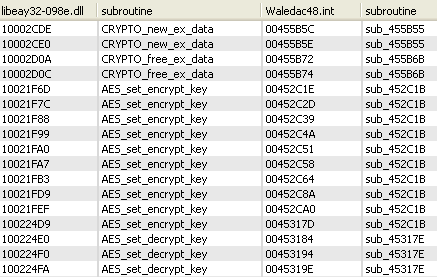
\includegraphics[width=0.8\textwidth]{supports/libs/WalSSLIDA2.png}
% \end{center}
% \caption{Fonctions correspondantes entre OpenSSL à gauche et Waledac à droite}
% \label{fig:plugin_subroutines}
% \end{figure}

\begin{figure}[h]
\begin{center}
\begin{tabular}{|l|l|l|l|}
\hline
\multicolumn{2}{|c|}{OpenSSL (libeay32-098e.dll)} & \multicolumn{2}{c|}{Waledac (Waledac48.int)} \\
\hline
Adresse & Fonction & Adresse & Fonction \\
\hline
 10002CDE & CRYPTO\_new\_ex\_data & 00455B5C & sub\_455B55 \\
 10002CD0 & CRYPTO\_new\_ex\_data & 00455B5E & sub\_455B55 \\
 10002D0A & CRYPTO\_new\_ex\_data & 00455B72 & sub\_455B55 \\
 10002D0C & CRYPTO\_new\_ex\_data & 00455B74 & sub\_455B55 \\
\hline
 10021F6D & AES\_set\_encrypt\_key & 00452C1E & sub\_452C1B \\
 10021F7C & AES\_set\_encrypt\_key & 00452C2D & sub\_452C1B \\
 10021F88 & AES\_set\_encrypt\_key & 00452C39 & sub\_452C1B \\
 10021F99 & AES\_set\_encrypt\_key & 00452C4A & sub\_452C1B \\
 10021FA0 & AES\_set\_encrypt\_key & 00452C51 & sub\_452C1B \\
 10021FA7 & AES\_set\_encrypt\_key & 00452C58 & sub\_452C1B \\
 10021FB3 & AES\_set\_encrypt\_key & 00452C64 & sub\_452C1B \\
 10021FD9 & AES\_set\_encrypt\_key & 00452C8A & sub\_452C1B \\
 10021FEF & AES\_set\_encrypt\_key & 00452CA0 & sub\_452C1B \\
 100224D9 & AES\_set\_encrypt\_key & 0045317D & sub\_452C1B \\
\hline
 100224E0 & AES\_set\_decrypt\_key & 00453184 & sub\_45317E \\
 100224F0 & AES\_set\_decrypt\_key & 00453194 & sub\_45317E \\
 100224FA & AES\_set\_decrypt\_key & 0045319E & sub\_45317E \\
\hline
\end{tabular}
\end{center}
\caption{Fonctions correspondantes entre OpenSSL et Waledac}
\label{fig:plugin_subroutines}
\end{figure}


Nous avons ensuite vérifié dans IDA, grâce à la fonction d'alignement de code du greffon, que le code des instructions correspondantes était bien suffisamment similaire pour valider la méthode.
Une telle correspondance est donnée en exemple à la figure \ref{fig:plugin_code_sync} pour la fonction \emph{AES\_set\_encrypt\_key}.
L'image est constituée d'un bout du graphe de flot de contrôle d'OpenSSL à gauche et d'un bout du GFC de Waledac à droite.
Les instructions surlignées en orange et alignées sont celles pour lesquelles on a trouvé une correspondance.

\begin{figure}[h]
\begin{center}
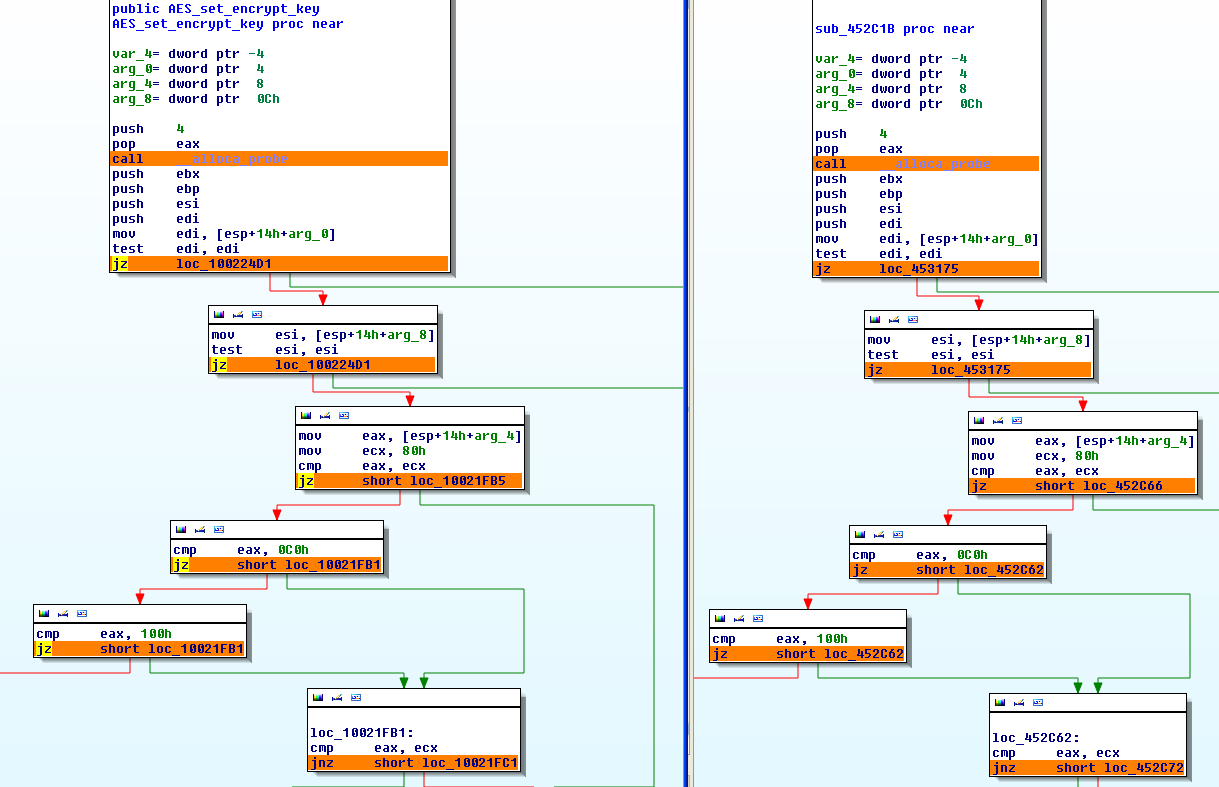
\includegraphics[width=1.0\textwidth]{supports/libs/WalSSLIDAAESgraph.png}
\caption{Capture d'écran d'IDA : Code correspondant entre OpenSSL à gauche et Waledac à droite} 
\label{fig:plugin_code_sync}
\end{center}
\end{figure}

Sur cet exemple nous n'avons pas trouvé de correspondance sommet à sommet qui ne soit pas cohérente mais certaines fonctions n'étaient pas couvertes par suffisamment de sommets pour que l'on soit assuré d'une correspondance.
La figure \ref{fig:tab_fonctionnalites_waledac_openssl} donne un extrait des fonctions d'OpenSSL retrouvées dans Waledac et les fonctionnalités qu'elles fournissent : on y trouve par exemple des méthodes préparant au chiffrement AES, RSA et DSA.

\begin{figure}[h]
\begin{tabular}{|p{9cm}|l|}
\hline
Fonctions 							& Fonctionnalité 			\\
\hline
AES\_set\_encrypt\_key, AES\_set\_decrypt\_key 			& Chiffrement AES 			\\
RSA\_free, DSA\_size, DSA\_new\_method 				& Chiffrement RSA / DSA 		\\
 X509\_PUBKEY\_set, X509\_PUBKEY\_get 				& Certificats X509 			\\
BN\_is\_prime\_fasttest\_ex, BN\_ctx\_new, BN\_mod\_inverse	& Gestion des grands entiers (BN)	\\
CRYPTO\_lock, CRYPTO\_malloc 					& Fonctions génériques d'OpenSSL 	\\
\hline
\end{tabular}
\caption{Fonctions d'OpenSSL retrouvées dans Waledac et fonctionnalités associées}
\label{fig:tab_fonctionnalites_waledac_openssl}
\end{figure}

Il n'est pas surprenant que l'on retrouve ces fonctionnalités puisque Waledac utilise du chiffrement AES et RSA et gère des certificats X509. Notre contribution est l'emploi de la technique d'analyse morphologique pour déterminer automatiquement ces informations sans analyser manuellement le code assembleur.

\section{Limites}
On a vu qu'on retrouve certaines fonctions utilisées lors d'un chiffrement AES.
Pourtant nous n'avons pas retrouvé les fonctions principales servant à chiffrer et déchiffrer à l'aide de l'algorithme AES.
La raison est que notre approche par graphes de flot réduits s'applique très mal aux fonctions de chiffrement qui sont en général très simples du point de vue de leur graphe de flot de contrôle.
Une vue simplifiée du GFC de la fonction \emph{AES\_encrypt} est donnée en figure \ref{fig:AES_encrypt_CFG}.

\begin{figure}[h]
\begin{center}
% \subfigure[AES\_encrypt subroutine]{
% 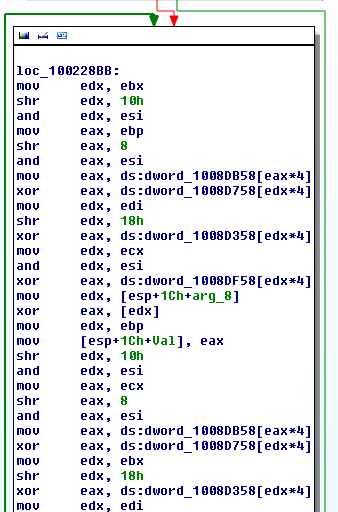
\includegraphics[width=0.4\textwidth]{supports/libs/WalSSLIDAAESencryptnotmatched.png}
% \label{fig:AES_encrypt_IDA}
% }
% \subfigure[]{
\includegraphics[width=0.25\textwidth]{supports/libs/AESsimpleCFG_cropped0.pdf}

% }
\end{center}
\caption{GFC simplifié de la fonction AES\_encrypt}
\label{fig:AES_encrypt_CFG}
\end{figure}

Le GFC réduit est trop petit pour pouvoir être détecté par l'analyse morphologique qui prend des graphes d'une taille 24 au minimum.
En fait beaucoup d'algorithmes de chiffrement ont cette structure une fois réduits et elle n'est pas non plus spécifique aux algorithmes de chiffrement. De ce fait l'analyse morphologique est inadaptée à la détection de ce genre de fonctions.

\section{Application à Duqu et Stuxnet}
Dans cette section nous présentons nos travaux sur deux programmes malveillants particuliers, \duqu\ et \stux.
Lorsque nous avons commencé ces travaux \stux\ était déjà documenté et détecté et \duqu\ venait d'être découvert.
Il a rapidement été dit qu'ils étaient semblables et nous avons donc cherché à détecter \duqu\ connaissant \stux.
% Dans un premier temps nous appliquons les travaux présentés au chapitre précédent sur ces exemples \cite{REAT12,mal12}.

\subsection{Duqu et Stuxnet}
% \paragraph{\stux.}
\stux, découvert en juin 2010, est capable de cibler et de reprogrammer des systèmes industriels.
Sans que cela ait été prouvé, il a été avancé qu'il visait le programme nucléaire iranien. 
Symantec \cite{SymantecStux2011} indique que la plupart des systèmes infectés sont en Iran et que la cible pourrait être un système de contrôle de centrifugeuses.
\\

% \paragraph{\duqu.}
\duqu, découvert en premier par Crysys \cite{CrysysDuquStuxnet} en septembre 2011, laboratoire de sécurité et de cryptographie de l'université de Budapest, a directement été détecté comme apparenté à \stux\ parce que ces deux programmes utilisent des techniques d'infection et de propagation similaires.
\duqu\ est un outil offensif utilisé pour le vol d'informations. Symantec \cite{SymantecDuqu2011} a identifié parmi ses fonctionnalités des enregistreurs de frappes (\emph{keyloggers}), de l'écran, de l'activité réseau ainsi que des outils de détection de machines sur le réseau.
Il est maintenu à jour via des serveurs de commande et de contrôle (C\&C) et dispose d'une fonctionnalité d'auto-destruction après, typiquement, 36 jours sans nouvelles du C\&C.

Les attaques semblent réussies puisque le programme malveillant n'a pas été détecté à chaud alors que certaines opérations ont duré plusieurs mois, mais seulement post-mortem. De nombreuses souches de \duqu\ ont été trouvées dans la natures, chacune avec des binaires différents mais similaires. Kaspersky a publié un historique des versions \cite{KaspDuqu10}, la dernière souche détectée date de février 2012, bien après que les première attaques n'ont été détectées et documentées.

\paragraph{Analyse des similarités.}
Nous avons effectué une analyse similaire à celle décrite au chapitre précédent pour trouver les similarités entre \stux\ et \duqu\ afin de trouver les parties de \stux\ que l'on retrouve dans \duqu.
Pour ces deux programmes malveillants, nous avons analysé la DLL (bibliothèque logicielle au format Windows, ou \emph{Dynamic Link Library}) principale une fois que celle-ci a été déchiffrée.
% Dans les deux cas l'infection est cherche à exploiter une faille de Windows permettant d'installer plusieurs composants qui auront été déchiffrés au préalable.
Nous avons extrait les graphes de flot réduits de \duqu\ et \stux.
Nous avons trouvé 846 sites communs entre \duqu\ et \stux\ : 26.5\% des sites de \duqu\ proviennent de \stux.
Lorsque l'on regarde les sommets correspondants dans les graphes réduits, on s'aperçoit que ces sites contiennent 2215 sommets dans les graphes de flot réduits : 60.3\% des sommets du graphe de flot réduit de \duqu\ correspondent à des sommets  présents dans \stux.

Forts de ces résultats indiquant que \duqu\ et \stux\ partagent beaucoup de code, nous considérons donc qu'un détecteur de programmes malveillants fonctionnant avec la technique d'analyse morphologique connaissant \stux\ serait capable de détecter \duqu.

La principale difficulté que doit résoudre un détecteur est que le programme provocant l'infection de \duqu\ ne ressemble pas à \stux\ ni à aucun autre programme malveillant connu. Ce n'est que lorsque certains composants de \duqu\ sont déchiffrés et installés que l'on peut le détecter.
Nous détaillons dans le chapitre suivant la méthode d'infection de \duqu\ et le travail nécessaire afin de détecter une attaque.
% Nous avons alors cherché à documenter la méthode d'infection de \duqu\ afin de pouvoir détecter une attaque.


\section{Perspectives}
Un approfondissement de cette approche à l'analyse de similarités logicielles serait intéressant. D'une part nous voudrions effectuer des expériences sur plus d'échantillons de code malveillant pour confirmer les résultats prometteurs mis en lumière dans ce chapitre.
D'autre part nous souhaiterions comparer en détail notre approche à celles existantes, notamment par rapport à une comparaison directe des instructions des binaires.

\section*{Conclusion}
Nous avons identifié des similarités entre Waledac et une version spécifique d'OpenSSL, nous avons pu reconstruire automatiquement des correspondances fines afin de déterminer quelles fonctions d'OpenSSL ont été utilisées par Waledac.
L'obstacle principal à une généralisation de cette méthode est qu'elle est sensible aux options de compilation et nécessite de déterminer au préalable les binaires à comparer.
Cette technique n'est pas infaillible puisqu'elle n'est pas adaptée pour détecter certaines structures ou fonctions, telles des fonctions de chiffrement.

Nous avons ensuite développé un greffon pour IDA permettant d'analyser les similarités trouvées afin de permettre à l'analyste de ne pas s'attarder sur du code déjà documenté.
Cette approche, appliquée à \duqu\ et \stux\ nous a permis de mettre en lumière de nombreuses portions de code partagées entre ces deux logiciels malveillants.

\DontFrameThisInToc
\chapter{Cas d'étude : Duqu et Stuxnet\label{chap:duqu-stux}}
Dans ce chapitre nous continuons nos travaux sur deux programmes malveillants particuliers, \duqu\ et \stux, dont nous avons montré qu'ils partageaient du code au chapitre précédent.
Notre objectif est de pouvoir détecter une attaque par \duqu\ connaissant \stux.
% cela nécessite un accès au code déchiffré et injecté par \duqu.

Nous cherchons donc à détecter \duqu\ avant qu'il ne puisse infecter une machine ciblée.
Nous étudions pour cela un composant spécifique de \duqu, son pilote (\emph{driver}) qui permet de charger discrètement le code malveillant en mémoire.
Notre contribution consiste en la rétroingénierie de ce composant, en la reconstitution de son code source et en une analyse de son fonctionnement.
Nous avons détournons ensuite le pilote pour en faire une version défensive capable de détecter d'éventuelles attaques similaires.
En particulier nous montrons comment le pilote de \duqu\ modifié permet de détecter et d'empêcher une attaque par \duqu.
Ces travaux ont fait l'objet d'une publication à SSTIC \cite{sstic13} ainsi qu'à  Malware \cite{mal13}.

\section{Détection d'une infection par Duqu}
\subsection{Déroulement d'une infection}
L'infection détectée par Crysys utilise un document Microsoft Word piégé, incluant \duqu.
Dans un premier temps il exploite une faille jusque là inconnue (\emph{0-day} sur les polices d'écriture TrueType \cite{CVETrueType}) du noyau Windows afin d'installer trois composants sur le système :
\begin{itemize}
 \item Un pilote : \driver
 \item Une DLL chiffrée : \netpDLL
 \item Un fichier de configuration chiffré : \netpCONF
\end{itemize}

Au redémarrage de la machine, le pilote surveille le chargement des processus par le système d'exploitation et injecte la DLL principale de \duqu, une fois déchiffrée, dans un processus spécifié par le fichier de configuration, typiquement \services.
Enfin le pilote modifie \services\ afin qu'il exécute la charge finale, qui est incluse dans la DLL.

Une fois installé sur une première cible \duqu\ reçoit des ordres d'attaque et de propagation d'un serveur C\&C.
Chaque machine infectée peut être configurée pour se connecter à l'attaquant, pas directement mais par la machine qui l'a infectée, créant une sorte de tunnel de routage pour des machines non accessibles directement depuis l'extérieur. Une illustration de ce mécanisme est donnée en figure \ref{fig:propagationDuqu}.

\begin{figure}[h]
\begin{center}
 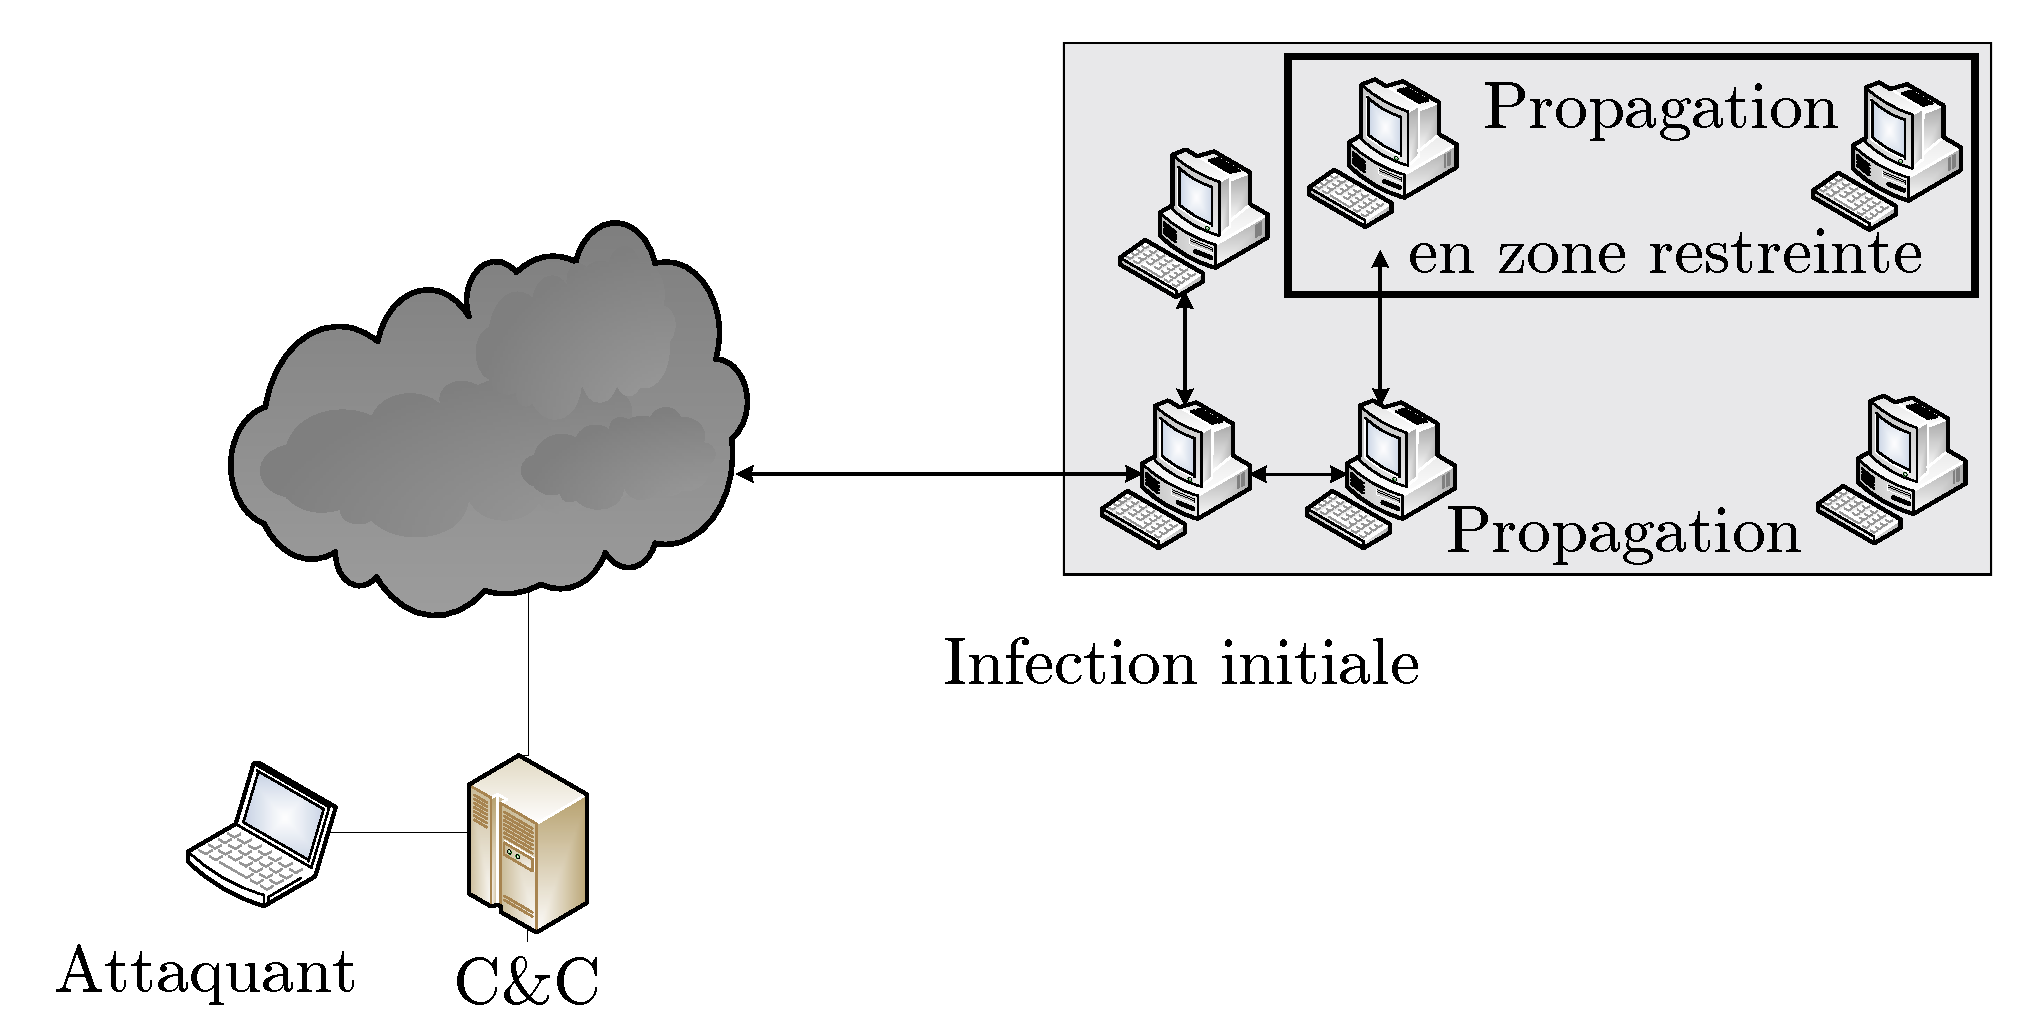
\includegraphics[width=0.8\textwidth]{supports/duqu/propagationDuqu2.pdf}
 % graph11.eps: 0x0 pixel, 300dpi, 0.00x0.00 cm, bb=0 0 384 336
\end{center}
\caption{Schéma de propagation en profondeur de Duqu}
\label{fig:propagationDuqu}
\end{figure}

\paragraph{Difficulté de la détection.}
L'obstacle principal à la détection est que seul le pilote est présent déchiffré sur le disque.
La DLL est chiffrée et empaquetée avec UPX, elle n'apparaît déchiffrée qu'en mémoire, lorsqu'elle est injectée dans \services.

\paragraph{Angle d'attaque pour une détection.}
L'attaque peut être détectée au moment du déchiffrement de la DLL principale et de son injection.
Elle doit prendre place après le déchiffrement mais avant que la charge finale ne soit exécutée.
Nous aurons pour cela besoin de suivre les processus lancés et de pouvoir analyser les DLL qu'ils exécutent.
Étant donné que le pilote de \duqu\ réalise cette opération, nous avons choisi de le modifier de telle sorte qu'il puisse s'interfacer avec le détecteur par analyse morphologique.
Pour mettre ce plan en \oe uvre, nous avons
\begin{itemize}
 \item reconstitué, par rétroingénierie, le code source du pilote de \duqu\ à partir de son binaire.
 \item modifié son code pour qu'il surveille le chargement des processus sans provoquer d'injection.
%  \item Interfacé le nouveau pilote avec notre outil de détection.
\end{itemize}

\subsection{Reconstruction du code du pilote}
Nous savions donc que les DLL principales de \duqu\ et \stux\ partageaient du code.
Le pilote de \stux\ a été décompilé par Amr Thabet \cite{ThabetDriver}.
Nous avons voulu suivre la même route et désassembler le pilote de \duqu\ afin de le documenter.
Nous avons eu à notre disposition la souche du pilote découverte en octobre 2011 en Europe : \driver.

Nous avons donc travaillé sur la rétroingénierie de cette version spécifique du pilote afin d’en documenter les fonctionnalités. 
Notre objectif est d’obtenir un code compréhensible que l'on peut compiler et dont la version compilée soit au plus proche du binaire d'origine.

\subsubsection{Décompilation avec IDA}
Nous avons utilisé le module de décompilation "Hex-Rays Decompiler", intégré à IDA sous la forme d’un greffon \cite{IDADecompiler}.
Il permet de générer un pseudo-code C à partir du fichier binaire en cours d’analyse.
Il produit non seulement du code source mais facilite également sa réécriture directement à l’intérieur de l’interface graphique du greffon. 
Malheureusement le code en sortie n’est, dans notre cas, pas exploitable directement. 
D’une part le code n’est pas compilable parce que des types de variables n’ont pas été correctement reconnus et certaines conventions d’appel ne sont pas standard (non reconnues par le décompilateur). 
De plus le code généré est difficilement lisible en partie parce que certaines structures n’ont pas été identifiées.
Nous détaillons dans les paragraphes suivants ces difficultés et des moyens de résolution.

Nous avons procédé de manière incrémentale afin de reconstruire le code petit à petit en vérifiant à chaque étape que le code compile et qu'une fois compilé il est équivalent à celui du binaire \driver\ original. 
Cela a consisté à :
\begin{itemize}
 \item commenter tout le pseudo-code sauf la fonction du point d'entrée du pilote (\emph{DriverEntry}) et les variables globales s'y rapportant,
 \item régler chaque erreur une par une,
 \item comparer le code compilé au binaire original, modifier le code pour s'en rapprocher,
 \item ajouter du code auparavant commenté et revenir à l'étape de correction d'erreurs.
\end{itemize}

\subsubsection{Identification des structures et des types}
La figure \ref{fig:ParsePEInitial} montre les premières lignes du code C reconstruit par le décompilateur pour une des fonctions du pilote.
Beaucoup d'informations manquent. Par exemple la plupart des types sont décrits comme des entiers (ou des pointeurs) : il n'est pas possible de savoir quel type de données cette fonction manipule.
Nous allons détailler sur cet exemple quelques techniques permettant de récupérer ces informations.

\begin{figure}[h]
\begin{center}
\begin{lstlisting}[language={C}]
signed int __cdecl sub_12F36(int a1, int a2, int a3)
{
  int v4; // eax@3
  unsigned __int16 v5; // cx@4
  int v6; // ecx@7

  v4 = a2 + *(_DWORD *)(a2 + 60);
  if (*(_DWORD *)v4 ^ 0xF750F284 != 0xF750B7D4)
    return 1;
\end{lstlisting}
\end{center}
\caption{Premières lignes de la fonction ParsePE décompilée par IDA\label{fig:ParsePEInitial}}
\end{figure}

Certaines constantes peuvent nous aider : par exemple \texttt{0xF750F284 XOR 0xF750B7D4 = 0x00004550} , qui représente la chaîne de caractères 'PE$\backslash$0$\backslash$0' en ASCII. Le texte est obscurci à l'aide d'une opération de ou exclusif (\emph{XOR}).

Nous soupçonnons alors que cette fonction est utilisée pour le traitement de fichiers binaires au format PE.
La documentation officielle de Microsoft Visual C++ détaille la structure PIMAGE\_NT\_HEADERS dont le premier champ, \emph{Signature}, vaut \PEzz\ pour les binaires Windows.
Ainsi la variable \texttt{v4}, qui est comparée à \PEzz, est probablement du type PIMAGE\_NT\_HEADERS.
Nous forçons ce type pour cette variable au sein d'IDA à la place du type \texttt{int} et IDA trouve automatiquement le nom des champs de ce type de variable à partir de leur décalage (\emph{offset}) en mémoire.
Lorsque les structures sont spécifiques au binaire analysé, il est possible de les définir manuellement dans le décompilateur.
Nous avons retrouvé les types des autres variables de manière similaire.

La figure \ref{fig:ParsePEFinal} donne les premières lignes de la fonction retouchée.
Elle est lisible par un développeur C : on peut voir que la fonction vérifie si un fichier est binaire PE.
Le reste de la fonction parcourt le binaire PE passé en entrée et remplit une structure spécifique avec quelques informations (son point d'entrée, ses sections, etc.).
De plus le code compilé de cette fonction est très similaire au binaire d'origine.


\begin{figure}[h]
\begin{center}
\begin{lstlisting}[language={C}]
NTSTATUS __cdecl ParsePE(__out PEDataPtr pPEData, 
    __in PIMAGE_DOS_HEADER BaseAddress, __in int flag){
PVOID infosPE;
PIMAGE_DOS_HEADER pDosHeader;
PIMAGE_NT_HEADERS pNtHeader;

pNtHeader = (DWORD)infosPE + infosPE->e_lfanew;
if ((pNtHeader->Signature ^ 0xF750F284) 
      != (IMAGE_NT_SIGNATURE ^ 0xF750F284)) 
    return STATUS_WAIT_1; 
\end{lstlisting}
\end{center}
\caption{Premières lignes de la fonction ParsePE reconstruite\label{fig:ParsePEFinal}}
\end{figure}

\subsubsection{Conventions d'appel}

Pour chaque routine IDA cherche à déterminer la convention d'appel utilisée à partir des registres qui sont lus avant d'être écrits (paramètres) et ceux écrits sans être lus après (valeur de retour). Si ces registres correspondent à un appel classique, IDA l'annote dans le code C pour que le compilateur respecte la convention. Les conventions d'appel de Microsoft Visual C++ sont données Figure \ref{fig:callingconvention}, l'appel par défaut étant \emph{thiscall}. Dans le cas où il ne détermine pas la convention, il annote les registres d'entrée et de sortie en notant qu'il s'agit d'un appel non conventionnel (\emph{usercall}) et met la définition de la fonction en commentaire (ici les arguments sont passés dans les registres \texttt{edi} et \texttt{esi}) :
\begin{small}
\begin{lstlisting}[language={C}, escapechar=!]
!//! int __usercall SearchForCode<eax>(int *a1<edi>, int a2<esi>);
\end{lstlisting}
\end{small}

Une convention d'appel non standard est détectée dans le cas où une partie de la fonction a été écrite directement en assembleur ou à la suite d'une optimisation faite par le compilateur. On doit alors réécrire, en partie en assembleur, la fonction sans passer par le décompilateur ou choisir une convention d'appel soi-même.

\begin{figure}[h]
\begin{center}
\begin{tabular}{|l|c|c|c|c|}
\hline 
Convention & Arguments & \emph{this} (C++) & Retour & Nettoie la pile\\
\hline
C (\_\_cdelcl) & pile & (argument) & eax & appelant\\
Standard (\_\_stdcall) & pile & (argument) & eax & appelé\\
Thiscall (\_\_thiscall) & pile & ecx & eax & appelé\\
Fastcall (\_\_fastcall) & ecx, edx, pile & (argument) & eax & appelé\\
\hline
\end{tabular}
\end{center}
\caption{Conventions d'appel dans leur version Visual C++}
\label{fig:callingconvention}
\end{figure}

Nous avons réalisé ce type d'analyse sur l'ensemble du pilote afin d'en reconstruire une version compréhensible et cohérente du code source du pilote.

\section{Analyse fonctionnelle du pilote de Duqu à partir du code source}
Une fois le code du pilote reconstitué, nous l'avons donc analysé.
Il y a deux phases principales, la première consiste en la mise en place du pilote : il demande au système à être notifié en cas de chargement de binaires et initialise ses mécanismes de furtivité.
La seconde phase est lancée lorsqu'une notification est signalée au chargement d'un des binaires ciblés : le pilote infecte alors le binaire en y injectant la DLL du \duqu\ puis celle-ci active la charge finale.

\subsection{Initialisation du pilote lors du démarrage du système}
Sous Windows l'ordre de démarrage des pilotes est déterminé par leur clé de registre \texttt{Group}.
Le pilote \driver\ de \duqu, appartenant au groupe ``network'', est activé avant même que la couche d'abstraction matérielle (\emph{HAL}) ne soit chargée en mémoire.

Le pilote, une fois démarré, commence par allouer un emplacement mémoire de 512 octets destiné à contenir un tableau de pointeurs de fonctions partagées entre les différentes routines de rappel (\emph{callback}) qui seront définies par la suite.
Il passe ensuite au déchiffrement de quelques paramètres internes, révélant le nom et l'emplacement de la clé de registre utilisée pour la configuration de l'injection.

Si le déchiffrement s'est correctement déroulé, vient alors la vérification du mode d'exécution : soit le système s'avère être en mode sans échec ou en mode débogage, dans ce cas le pilote termine prématurément son exécution ; soit il est en mode normal, le pilote crée alors un \emph{device}, \texttt{\{624409B3-4CEF-41c0-8B81-7634279A41E5\}}, et définit la liste des commandes de contrôle qu'il sera amené à traiter.

Cette étape réalisée, le pilote enregistre deux fonctions de rappel auprès du gestionnaire d'événements interne du noyau.
La première est requise par le système : elle est utilisée pour créer un point d'accès ($\backslash$\texttt{Device}$\backslash$\texttt{Gpd0}) et un lien ($\backslash$\texttt{DosDevices}$\backslash$\texttt{GpdDev}) vers le pilote ainsi que pour définir une pile mémoire pour le \emph{device}.
La seconde fonction sera appelée lorsque le pilote sera initialisé ou ré-initialisé. 


Cette seconde fonction attend que le noyau Windows soit complètement chargé en vérifiant si la DLL \texttt{hal.dll} est chargée en mémoire. Lorsque le système est prêt, un point d'accès, $\backslash$\texttt{Device}$\backslash$\texttt{Gpd1}, est créé et lié à une routine de traitement des requêtes. 
À ce stade le pilote est prêt à réaliser l'injection.

\subsubsection{Techniques de furtivité}
Le pilote agit désormais furtivement (on parle de \emph{rootkit}) et évite d'utiliser directement des appels systèmes connus pour être sensibles, utilisés par des logiciels malveillants, et probablement surveillés par un éventuel antivirus.
La fonction \ZwA\ peut être utilisée pour allouer de la mémoire au sein d'un processus au choix, pour y injecter du code arbitraire par exemple.
De plus, afin de détourner le point d'entrée d'un binaire (\emph{hook}), \duqu\ veut également utiliser la fonction \ZwP\ que Microsoft a délibérément omise de la liste des fonctions accessibles en dehors du noyau. Cette fonction permet de modifier les permissions d'une page mémoire et peut être utilisée pour rendre une partie de code accessible en écriture ou rendre une section de données exécutable.

Ces deux fonctions sont implémentées dans le noyau Windows, dans les fichiers \path{Ntoskrnl.exe} ou \path{ntkrnlpa.exe}, selon les versions. 
Le pilote inspecte chaque module, DLL et exécutables, chargés par le système lors du démarrage à la recherche d'un de ces deux fichiers.

Une fois le fichier cible trouvé, le pilote utilise la fonction \emph{ParsePE} pour l'examiner et y retrouver l'adresse de \ZwP.
Pour cela il dispose d'un motif à reconnaître.
Il est à la recherche d'un appel vers \ZwA, dont l'adresse est connue parce qu'elle est présente dans la table d'exports du noyau, suivi par l'instruction \texttt{push 0x104} et par une instruction \texttt{call}.
Si ce motif, représenté en figure \ref{fig:CallZwProtect}, est retrouvé alors l'adresse cible de ce \texttt{call} est considérée comme étant \ZwP.
À partir de cet instant, le pilote connaît les adresses mémoires de ces deux fonctions.

\begin{figure}[h]
\begin{center}
\scriptsize
\begin{lstlisting}[language={[x86masm]Assembler}, escapechar=~]
(01) PAGE:004ED1AD                  loc_4ED1AD: [...]                      
(02) PAGE:004ED1BC 50               push    eax             ; BaseAddress
(03) PAGE:004ED1BD 57               push    edi             ; ProcessHandle
(04) PAGE:004ED1BE E8 19 8C F1 FF   ~\textcolor{red}{\texttt{call    DS:ZwAllocateVirtualMemory}}~
(05) PAGE:004ED1C3 3B C3            cmp     eax, ebx
(06) PAGE:004ED1C5 8B 4D FC         mov     ecx, [ebp+BaseAddress]
(07) PAGE:004ED1C8 89 4E 0C         mov     [esi+0Ch], ecx
(08) PAGE:004ED1CB 7C 2E            jl      short loc_4ED1FB
(09) PAGE:004ED1CD 38 5D 0B         cmp     byte ptr [ebp+ProcessHandle+3], bl
(10) PAGE:004ED1D0 74 27            jz      short loc_4ED1F9
(11) PAGE:004ED1D2 8B 45 D0         mov     eax, [ebp+var_30]
(12) PAGE:004ED1D5 89 45 F8         mov     [ebp+ProtectSize], eax
(13) PAGE:004ED1D8 8D 45 F4         lea     eax, [ebp+OldProtect]
(14) PAGE:004ED1DB 50               push    eax             ; OldProtect
(15) PAGE:004ED1DC 68 04 01 00 00   ~\textcolor{red}{\texttt{push    104h}}~
(16) PAGE:004ED1E1 8D 45 F8         lea     eax, [ebp+ProtectSize]
(17) PAGE:004ED1E4 50               push    eax             ; ProtectSize
(18) PAGE:004ED1E5 8D 45 FC         lea     eax, [ebp+BaseAddress]
(19) PAGE:004ED1E8 50               push    eax             ; BaseAddress
(20) PAGE:004ED1E9 57               push    edi             ; ProcessHandle
(21) PAGE:004ED1EA E8 93 96 F1 FF   ~\textcolor{red}{\texttt{call    loc\_406882}}~ ; ZwProtectVirtualMemory
(22) PAGE:004ED1EF 3B C3            cmp     eax, ebx
\end{lstlisting}
\end{center}
% \end{framed}
\caption{Fonction faisant appel à \ZwP\label{fig:CallZwProtect}}
\end{figure}

\paragraph{Vérification d'intégrité.}
Le pilote cherche à détecter si les fonctions \ZwA\ et \ZwP\ ont été la cible d'un détournement défensif par un antivirus cherchant à les surveiller.
Il vérifie dans un premier temps que les deux fonctions sont présentes dans l'espace mémoire du noyau et non en espace utilisateur.
Dans un second temps il leur applique un masque d'intégrité vérifiant la valeur d'une partie des 20 premières adresses mémoires sur lesquelles les deux fonctions sont codées. Le masque est le même pour les deux fonctions et est donné en figure \ref{fig:masque_integrite}.
Si les fonctions passent le test, leurs adresses sont considérées valides et sont conservées pour une future utilisation discrète.


\begin{figure}[h]
\begin{center}
% Masque d'intégrité :\\
\begin{tabular}{|c|c|c|c|c|c|c|c|c|c|}
\hline
b8\cgris & ~~ & ~~ & ~~ & ~~ & 8d\cgris & 54\cgris & 24\cgris & 04\cgris & 9c\cgris \\
\hline
6a\cgris & 08\cgris & e8\cgris & ~~ & ~~ & ~~ & ~~ & c2\cgris & 14\cgris & ~~\\
\hline
\end{tabular}
\end{center}

\begin{center}
\ZwA:\\
\begin{tabular}{|l|c|c|c|c|c|l|}
\hline
\adr{405ddc} & b8\cgris & 11 & 00 & 00 & 00 & mov eax, 0x11 \\
\hline
\adr{405de1} & 8d\cgris & 54\cgris & 24\cgris & 04\cgris & ~~ & lea edx, [esp+ProcessHandle] \\
\hline
\adr{405de5} & 9c\cgris & ~~ & ~~ & ~~ & ~~ & pushf \\
\hline
\adr{405de6} & 6a\cgris & 08\cgris & ~~ & ~~ & ~~ & push 8 \\
\hline
\adr{405de8} & e8\cgris & b9 & 20 & 00 & 00 & call +0x20be (sub\_407ea6) \\
\hline
\adr{405ded} & c2\cgris & 14\cgris & 00 & ~~ & ~~ & ret 0x14 \\
\hline
\end{tabular}
~\\~\\
\ZwP:\\
\begin{tabular}{|l|c|c|c|c|c|l|}
\hline
\adr{406882} & b8\cgris & 89 & 00 & 00 & 00 & mov eax, 0x89 \\
\hline
\adr{406887} & 8d\cgris & 54\cgris & 24\cgris & 04\cgris & ~~ & lea edx, [esp+ProcessHandle] \\
\hline
\adr{40688b} & 9c\cgris & ~~ & ~~ & ~~ & ~~ & pushf \\
\hline
\adr{40688c} & 6a\cgris & 08\cgris & ~~ & ~~ & ~~ & push 8 \\
\hline
\adr{40688e} & e8\cgris & 13 & 16 & 00 & 00 & call +0x1618 (sub\_407ea6) \\
\hline
\adr{406893} & c2\cgris & 14\cgris & 00 & ~~ & ~~ & ret 0x14 \\
\hline
\end{tabular}
\end{center}

\caption{Masque d'intégrité appliqué à \ZwA\ et \ZwP. Les valeurs grisées sont celles qui sont vérifiées.}
\label{fig:masque_integrite}
\end{figure}

\FloatBarrier
\subsubsection{Initialisation de la mémoire partagée}
Une mémoire partagée est allouée et utilisée comme lien entre les routines de rappel du pilote et le noyau.
Elle contiendra, entre autres, les paramètres pour l'infection déchiffrés depuis les données d'une clé de registre et une table d'imports donnant accès à la DLL \texttt{kernel.dll} et aux fonctions du noyau.
Cette table d'imports sera utilisée à la fois par le code que \duqu\ va injecter dans \services\ et par la charge finale.

La phase d'initialisation prend fin en mettant en place une notification système dès qu'un module (DLL ou exécutable) est chargé en mémoire, via l'appel système \textbf{PsSetLoadImageNotifyRoutine}.

\FloatBarrier
\subsection{Injection de code}
\subsubsection{Traitement de la première notification}
\paragraph{Préparation à l'injection.}
Le pilote est notifié à chaque fois qu'un module (DLL ou exécutable) est chargé en mémoire.
À chaque fois le pilote tente de localiser l'emplacement mémoire du module.
Pour cela il utilise l'identifiant du processus que lui fournit le système d'exploitation lors de la notification.
Il lit l'adresse de base du fichier directement à partir des informations accessibles dans la structure PEB (\emph{Process Environment Block}) et la compare à celle passée en paramètre par le système.
Il vérifie que le fichier de configuration est bien déchiffré dans la mémoire partagée et lit le champ donnant la cible de l'injection.
Comme expliqué dans le document de Crysys \cite{CrysysDuquStuxnet}, la cible est \services\ donc nous nous focalisons sur ce processus et l'injection dont il sera victime.

\paragraph{Injection de la charge finale.}
Le pilote de \duqu\ va maintenant injecter du code malveillant dans \services\ de telle manière que la charge finale soit exécutée par \services\ avant que son code légitime ne soit à son tour exécuté.

Une fois que \services\ est chargé, le pilote détermine son point d'entrée et alloue de la mémoire dans sa section \pdata\ à l'aide de la fonction \ZwA.
Deux fichiers PE dont les entêtes ont été altérés à des fins de furtivité sont injectés.
Ensuite certaines constantes ('\texttt{MZ}', '\texttt{IMAGE\_NT\_SIGNATURE}', '\texttt{IMAGE\_PE\_i386\_MACHINE}, et '\texttt{IMAGE\_PE32\_MAGIC}') du premier code injecté sont restaurées.
Certaines adresses sont recalculées : les adresses cibles de sauts qui étaient codées en dur doivent être recalculées.
Enfin le pilote modifie les permissions du point d'entrée de \services\ de \texttt{RX} (\texttt{PAGE\_EXECUTE\_READ}) à \texttt{RWX} (\texttt{PAGE\_EXECUTE\_WRITECOPY}) en utilisant la fonction \ZwP.

Le pilote \driver\ alloue alors de la mémoire dans le processus \services\ de la taille de la DLL déchiffrée \netpDLL\ augmentée de 57 octets.
Ensuite un gestionnaire d’événements (\emph{handler}) est ouvert sur le pilote et est sauvegardé dans la mémoire partagée afin de pouvoir être utilisé par le code injecté.

\subsubsection{Traitement de la seconde notification}
Le pilote n'est pas uniquement notifié quand le module principal (\services) est chargé mais également lorsque des DLL liées à ce module sont également chargées.
\idone{Les sigles ne prennent pas la marque du pluriel}
En particulier lorsque la DLL \texttt{kernel32.dll} est chargée, le pilote cherche les adresses de 10 de ses fonctions exportées qui seront utilisées par la charge finale.
Toujours dans une optique de furtivité la recherche consiste à comparer un haché cryptographique au nom de chacune des fonctions exportées par la DLL.
Cette étape se termine par une sauvegarde des 12 premiers octets présents au point d'entrée de \services\ et leur remplacement par un saut vers le premier code injecté et restauré.
Les premières instructions du point d'entrée sont changées en l'instruction \texttt{mov eax, @AdresseInjection} suivie de \texttt{call eax}.

Le processus \services\ a ainsi été altéré et est prêt à lancer la charge finale.

\subsubsection{Lancement de la charge finale}
Le système d'exploitation termine l'initialisation de \services\ et procède à son exécution en passant le contrôle au point d'entrée modifié, c'est à dire au premier code injecté par \duqu.

Sa première tâche consiste à déterminer sa propre adresse en mémoire afin de pouvoir recalculer les adresses de certaines cibles de saut.
Cette opération peut être effectuée à l'aide de deux instructions : un \texttt{call +5} vers l'instruction suivante suivi d'un \texttt{pop eax} a pour effet de placer l'adresse de retour (celle de \texttt{pop eax}) en haut de la pile puis de la dépiler dans \eax\ qui contient alors cette même adresse.
Il modifie alors les adresses à partir du nouveau point d'entrée déterminé.

Il restaure ensuite les entêtes du second PE injecté afin de le rendre valide et remplit, dans une structure partagée, une table d'import à partir des 10 fonctions trouvées précédemment de \texttt{kernel32.dll}.
Il crée ensuite un gestionnaire d’événements sur la DLL \texttt{ntdll.dll} qui est enregistré dans une structure partagée.
Il transfert ensuite le contrôle au point d'entrée sur second code injecté.

Ce module additionnel ajoute les données de son propre entête (adresse du module, nombre de sections, adresse de la table d'exports) dans la mémoire partagée.
Enfin ces informations sont utilisées pour charger ce PE manuellement en mémoire : les espaces mémoires sont alloués, l'entête est copié, les sections et les DLL liées sont chargées en mémoire, une table d'imports est créée, les adresses sont recalculées à partir de son point d'entrée.
Puis la DLL principale de \duqu, \netpDLL, est chargée et liée à ce PE et son point d'entrée est appelé.
La figure \ref{fig:ServiceMem} donne l'état du processus \services\ et de la mémoire à cette étape de l'injection.


\begin{figure}[h]
\begin{center}
\scalebox{1}{
\begin{tikzpicture}[->,scale=1,>=stealth',thick]
\node[state, align=left, text width=6cm, minimum size=1cm] (EP){\small Point d'entrée altéré:\\\adr{01012475} \texttt{mov eax, 0x0a18bd}\\\adr{0101247a} \texttt{call eax}};
\node[state, below=-0.05cm of EP.south, anchor=north, text width=6cm, minimum size=1cm] (TEXTP){...};
\node [fit={($(EP.north west) + (0.0, 0.4)$) ($(TEXTP.south east) + (0.0, 0.0)$)}, draw, dash pattern=on \pgflinewidth off 2pt, label={[xshift=1.2cm,yshift=-0.55cm]north west:\small Code}](TEXT) {};

\node[state, below=1cm of TEXTP.south, anchor=north, text width=6cm, minimum size=0.7cm] (PE1){PE injecté avec entêtes restaurés};
\node[state, below=0.1cm of PE1.south, anchor=north, text width=6cm, minimum size=0.7cm] (PE2){PE injecté avec entêtes restaurés};
\node [fit={($(PE1.north west) + (0.0, 0.4)$) ($(PE2.south east) + (0.0, 0.0)$)}, draw, dash pattern=on \pgflinewidth off 2pt, label={[xshift=1.7cm,yshift=-0.55cm]north west:\small Données}](DATA) {};

\node[state, below=1cm of PE2.south, anchor=north, text width=6cm, minimum size=0.7cm] (DLL){DLL déchiffrée};
% \node[state, below=0.1cm of PE1.south, anchor=north, text width=6cm, minimum size=0.7cm] (PE2){PE injecté avec entêtes restaurés};
\node [fit={($(DLL.north west) + (0.0, 0.4)$) ($(DLL.south east) + (0.0, 0.0)$)}, draw, dash pattern=on \pgflinewidth off 2pt, label={[xshift=0.9cm,yshift=-0.55cm]north west:\small Tas}](TAS) {};
\node [fit={($(TEXT.north west) + (0.0, 0.0)$) ($(TAS.south east) + (0.0, 0.0)$)}, draw, label=\services](SERVICES) {};

\node[state, right=1cm of SERVICES.east, anchor=west, text width=6cm, minimum size=0.7cm] (DUQUPE){PE};
\node[state, below=0.1cm of DUQUPE.south, anchor=north, text width=6cm, minimum size=0.7cm] (DUQUDLL){DLL};
\node [fit={($(DUQUPE.north west) + (0.0, 0.0)$) ($(DUQUDLL.south east) + (0.0, 0.0)$)}, draw, label=Charge finale de \duqu](DUQU) {};

% \node[state, text width=2cm, minimum size=3cm] (TEXT){Code};
% \node[state, below = -3cm of TEXT.north, text width=2cm, minimum size=3cm, anchor=north] (DATA){Données};
% \draw ($(BIN.east) + (0.5, 0) $) -- node[below]{\large Enpaquetage} ($(BIN.east) + (3cm, 0) $);
% \node [fit={($(UNPACK.north west) + (-0.1, 0.1)$) ($(BINO.south east) + (0.1, -0.1)$)}, draw, label=Binaire empaqueté] {};
\end{tikzpicture}
}
\end{center}
\caption{Mémoire de \services\ et de \duqu\ une fois que l'injection est complète}
\label{fig:ServiceMem}
\end{figure}

La charge finale contenue dans la DLL est maintenant en place et exécutée.
Une fois qu'elle a fini, elle envoie une requête au pilote via le point d'accès créé précédemment, \texttt{\{624409B3-4CEF-41c0-8B81-7634279A41E5\}}, afin qu'il restaure les 12 premiers octets du point d'entrée de \services.
Une seconde requête est envoyée pour restaurer les droits d'accès d'origine du point d'entrée de \services.

L'attaque ayant été réalisée, le contrôle est maintenant passé à \services, qui a été restauré et s'exécute cette fois normalement.

\section{Réalisation d'une version défensive}
Nous avons précédemment décrit comment la DLL de \duqu\ est injectée dans \services.
Certaines des techniques décrites, telle la mise en place de notifications au lancement de chaque module, peuvent être utilisées à des fin défensives.

Schématiquement, le pilote modifié va calculer des signatures sur les binaires chargés en mémoire.
Lorsqu'un binaire est lancé, dans le cas où sa signature n'est pas reconnue, il sera considéré suspect et stoppé.
Nous détaillons les phases d'initialisation, de mémorisation puis de détection implémentées dans le pilote modifié.
Nous terminerons ce chapitre par une présentation détaillée d'une exécution du binaire modifié en situation d'attaque par \duqu.

\subsection{Phase d'initialisation}
La phase d'initialisation d'origine a été grandement allégée pour notre pilote modifié.
Nous avons gardé la création des points d'accès, enlevé la recherche de la fonction \ZwP, que nous n'utiliserons pas.
Nous avons conservé le système de notification des chargements de modules en mémoire et avons également demandé de recevoir une notification lorsque le système termine la création d'un processus (à l'aide de la fonction \emph{PsSetCreateProcessNotifyRoutine}).

\subsection{Phase de mémorisation}
Nous avons vu que le point d'entrée n'est pas altéré lors de la première notification.
Ainsi si une somme de contrôle est calculée pour le point d'entrée de chaque module, la modification du point d'entrée peut être détectée lorsque la seconde notification sera déclenchée.
Nous avons intégralement repris la fonction de hachage implémentée dans \duqu\ qui était à l'origine utilisée pour obscurcir le nom des fonctions appelées.

Une première notification est reçue lorsque le processus est créé.
% Malheureusement Windows fournit uniquement l'identifiant du processus et son processus parent, mais pas d'informations sur l'emplacement en mémoire du processus.
Nous récupérons la structure PEB (\emph{Process Environment Block}) associée à ce processus et l'utilisons pour récupérer l'adresse mémoire du module chargé.

Afin de détecter \duqu\ nous nous focalisons uniquement sur le processus \services\ ciblé.
Si le nom du processus chargé est ``\services '', nous recherchons son point d'entrée, nous calculons une somme de contrôle sur ses huit premiers octets et l'enregistrons comme signature initiale.
Le pilote défensif est maintenant prêt à détecter l'injection effectuée par \duqu.

\subsection{Phase de détection}
Lorsqu'un module est chargé, le système passe le contrôle au pilote défensif qui vérifie le point d'entrée du module.
Si le module est une DLL, le point d'entrée recherché est celui de l'exécutable auquel la DLL est associée.
Nous avons donc ajouté une vérification de la somme de contrôle.

Cette somme de contrôle est comparée à celle calculée en premier lieu.
Si elles diffèrent, nous considérons qu'une injection a eu lieu sur \services\ entre les deux notifications et, puisque son point d'entrée a été altéré, le processus \services\ est considéré comme suspect.


\subsection{Démonstration}
Pour faciliter la mise au point du pilote de détection, nous l'avons installé, ainsi que celui de \duqu, sur une machine de test en suivant la démarche proposée par Sergei Shevchenko \cite{SShevchenko}.
Nous renommons la calculatrice Windows (\texttt{calc.exe}) en \services\ et observons comment deux pilotes réagissent à son lancement.

Pour cette démonstration, nous avons utilisé deux machines virtuelles sous Windows XP SP3 connectées par un lien série.
Une instance de WinDbg \cite{WinDbg}, débogueur fonctionnant sur le noyau Windows, tourne sur la première machine.
La seconde machine est lancée en mode ``débogage du noyau'' l'autorisant à dialoguer avec la première machine afin que celle-ci puisse déboguer les pilotes du noyau.

Lors de ces tests nous avons observé que le pilote \driver\ de \duqu\ vérifie si le système est en mode débogage ou en mode sans échec : nous l'avons alors modifié pour qu'il se lance tout de même en mode débogage.
Nous avons également configuré les deux pilotes afin que l'on puisse les lancer sur demande (et non automatiquement au lancement de la machine).
Cette configuration nous permet de choisir l'ordre de lancement des pilotes ainsi que de \services.

\paragraph{Lancement du pilote défensif en premier.}
Nous lançons en premier le pilote défensif, puis celui de \duqu\ et enfin \services.
La sortie du débogueur est donnée en figure \ref{fig:Breakpoint1} : on voit le chargement de \services.
Le système notifie le pilote défensif qui enregistre l'identifiant, l'adresse du point d'entrée et la signature des premiers octets du point d'entrée de \services.

\begin{figure}[h]
\begin{center}
\scriptsize
\lstset{
  xleftmargin=.1\textwidth, xrightmargin=.1\textwidth
}
\begin{lstlisting}[language={}]
-----------------------+* Create process 0x914 *+------------------------
ProcessImageInformation: PEB=0x7ffd6000, ImageBaseAddress=0x01000000,
			 UniqueProcessId=0x914 
Entrypoint bytes at 0x01012475: 0x6a 0x70 0x68 0xe0 0x15 0x00 0x01 0xe8
ProcessImageName: Desktop\services.exe
ProcessImageName: save processID=0x914
CreateProcessNotify: ImageBaseAddress=0x01000000, EntryPoint=0x01012475,
		     EntrypointChecksum=0x49af1bf2
\end{lstlisting}
\end{center}
\caption{Sortie de WinDbg. Le processus \services\ est chargé : le pilote défensif enregistre son identifiant (\texttt{0x914}), son point d'entrée (\adr{01012475}) et sa somme de contrôle (\texttt{0x49af1bf2}).\label{fig:Breakpoint1}}
\end{figure}

Lorsque la notification pour \texttt{kernel32.dll} est déclenchée, aucune modification n'a encore été faite puisque \duqu\ reçoit la notification après le pilote défensif, car nous avons lancé le pilote défensif en premier.
La comparaison des sommes de contrôle ne détecte alors pas de différence.
Lorsque d'autres DLL liées à \services\ sont chargées, le pilote défensif vérifie à nouveau le point d'entrée qui a cette fois été altéré.
Le traitement des notifications liées aux DLL \texttt{kernel32.dll} et \texttt{shell32.dll} est montré en figure \ref{fig:Breakpoint2}.
Ainsi l'altération du point d'entrée est détecté et le pilote défensif prend une décision pour protéger le système : le processus \services\ est stoppé, arrêtant la tentative d'infection de la machine.


\begin{figure}[h]
\begin{center}
\scriptsize
\lstset{
  xleftmargin=.1\textwidth, xrightmargin=.1\textwidth
}
\begin{lstlisting}[language={}]
----------* Loaded module \WINDOWS\system32\kernel32.dll *----------
LoadImageNotifyRoutine: ImageBaseAddress=0x7c800000 ProcessId=0x914 
-> Verify services.exe process: 
   Entrypoint at 0x01012475: 0x6a 0x70 0x68 0xe0 0x15 0x00 0x01 0xe8
-> OK!

----------* Loaded module \WINDOWS\system32\shell32.dll *----------
LoadImageNotifyRoutine: ImageBaseAddress=0x7c9d0000 ProcessId=0x914 
-> Verify services.exe process:
   Entrypoint at 0x01012475: 0xb8 0xbd 0x18 0x0a 0x00 0xff 0xd0 0xe8
-> Checksum error !
-> Terminating services.exe
\end{lstlisting}
\end{center}
\caption{Détection de l'altération du point d'entrée (\adr{01012475}) de \services.\label{fig:Breakpoint2}}
\end{figure}

\paragraph{Lancement du pilote de \duqu\ en premier.}
Dans le cas où on lance le pilote du \duqu\ puis le pilote défensif, la première notification ne provocant pas de modification par le pilote de \duqu, la version défensive calcule toujours la somme de contrôle d'origine de \services.
Lors de la seconde notification, pour \texttt{kernel32.dll}, \duqu\ est injecté et le point d'entrée est modifié. Puis le pilote défensif est également notifié du chargement de \texttt{kernel32.dll} et détecte l'altération du point d'entrée, terminant cette fois aussi \services\ avant que la charge finale ne soit activée.

Au final, quel que soit l'ordre de chargement des pilotes, le pilote défensif permet d'éviter l'infection.
Il est à noter que ce comportement vient de l'utilisation par le pilote de \duqu\ de deux notifications pour faire son injection : s'il l'effectuait dès la réception de la première notification, l'ordre de chargement des pilotes deviendrait crucial et, si le pilote de \duqu\ était lancé en premier, nous ne serions pas capables d'empêcher l'infection.

\section{Perspectives}
Nous sommes capables de détecter l'injection de d'empêcher le chargement de \services\ afin d'éviter l'attaque.
Cela dit Windows ne peut pas fonctionner normalement sans \services. La machine ne sera donc pas infectée mais nécessitera une intervention humaine pouvant éventuellement détecter que le programme malveillant injecté est une variante de \stux.
Deux contributions supplémentaires pourraient être effectuées. D'une part nous voudrions analyser automatiquement la mémoire du processus infecté, \services, à la recherche de binaires connus pour être malveillants. 
Cette étape permettrait de trouver la DLL \netpDLL\ de \duqu\ et de la relier à \stux\ puisque l'analyseur morphologique est capable de détecter des similarités. Nous n'avons pas implémenté cette analyse.
D'autre part nous voudrions être capables de restaurer la version d'origine de \services\ afin que le système puisse non seulement éviter l'attaque mais également fonctionner dans un état normal.

\section*{Conclusion}
Des similarités entre \duqu\ et \stux\ nous ont poussés à nous intéresser à une technique de détection permettant de stopper une attaque par \duqu.
Nous avons décrit la technique d'infection ainsi que le fonctionnement du pilote de \duqu\ et ses méthodes pour rester furtif.
Nous avons ensuite reconstruit le code source du pilote de \duqu\ et en avons fait une version défensive capable de détecter l'injection faite par le logiciel malveillant et de stopper le processus infecté.

Ce travail de décompilation, d'analyse et de construction d'une version défensive de \duqu\ a principalement été orchestré et réalisé par Fabrice Sabatier que je tiens à remercier.


\DontFrameThisInToc
\chapter*{Conclusion et perspectives\label{chap:conclusion}}
\section*{Synthèse des travaux réalisés}
% \itodo{pb 0: analyse de programmes obfusqués}
% \itodo{pb 1: analyse du chevauchement de code}
% \itodo{pb 2: analyse/désassemblage des programmes sms}

Notre contribution à l’analyse de programmes obscurcis s'est concentrée sur l'analyse de deux techniques de protection : l'auto-modification et le chevauchement de code.
Nous avons décrit un langage assembleur disposant d’une sémantique concrète compatible avec l’exécution de programmes auto-modifiants.
Nous avons étendu BAP, une plateforme d’analyse de binaires existante, pour lui permettre d’évaluer des programmes auto-modifiants et de séparer des programmes simples en différentes vagues d'exécution.
Nous avons formalisé le problème du chevauchement de code et étudié l’usage que les programmes obscurcis font de cette méthode de protection. 
Enfin nous avons proposé une technique de désassemblage consistant à effectuer une analyse dynamique que l’on complète à l’aide de techniques d’analyse statique. 
Cette technique a pour objectif de reconstruire un graphe de flot de contrôle dont nous avons défini la forme idéale.
Nous avons implémenté un détecteur réalisant l'analyse dynamique à l'aide de l'outil d'instrumentation Pin et reconstruisant le graphe de flot de contrôle paramétré par cette exécution.
La pertinence de cet outil a été démontrée lors de l'analyse de programmes obscurcis.

Notre contribution à l’analyse morphologique consiste en la formalisant du sous-problème d’isomorphisme de sous-graphes qu’elle cherche à résoudre.
Nous avons proposé une alternative à l'algorithme d'Ullmann, fonctionnant par recherche de parcours au sein d'un graphe de flot.
Cette approche est aussi précise que les approches existantes mais est beaucoup plus rapide. Nous l'avons implémentée et avons également décrit et implémenté un second algorithme, incorrect, mais dont le temps d’exécution constant ne dépend pas du nombre de programmes présents dans la base de détection.
Nous avons enfin proposé une application de la technique d’analyse morphologique au domaine de la détection de similarités logicielles \cite{REAT12,mal12} et appliqué cette méthode pour analyser quelques logiciels malveillants spécifiques dont Duqu et Stuxnet \cite{sstic13,mal13}.

% Les programmes malveillants obscurcis sont notre objet d'étude principal.
% Notre objectif principal a été le désassemblage et la reconstruction du graphe de flot de contrôle d'un programme malveillant obscurci.
% Nous cherchions à contrer particulièrement deux méthodes d'obscurcissement. 
% La première est l'auto-modification, technique permettant aux programmes de cacher leur charge utile et de ne la révéler que juste avant son exécution. La seconde est le chevauchement de code, permettant à plusieurs instructions d'être codées sur des adresses communes.
% 
% Nous avons proposé une méthode d'analyse hybride, se basant sur une trace d'exécution, permettant de guider l'analyse statique.
% La trace d'exécution est récupérée, comme dans les travaux de Reynaud \cite{Reynaud2010}, par une analyse dynamique qui découpe l'exécution en parties successives, non auto-modifiantes, du programme, ou vagues.
% La trace restreinte à une vague ne présente pas d'auto-modification, ce qui permet l'emploi de méthodes d'analyse statique sur chacune des vagues.
% Cette analyse statique fait une utilisation intensive des informations contenues dans la vague afin de guider son analyse.
% Elle reprend certaines techniques détaillées par Krügel \cite{KruegelRVV04} mais fonctionne sur des binaires utilisant le chevauchement de code et permet d'en mesurer utilisation : nous avons proposé une sémantique pour le chevauchement de code rangeant les instructions dans des couches de code au sein desquelles il n'y a pas de chevauchement.
% 
% Nous avons implémenté cette technique d'analyse hybride et validé des expériences précédentes, comme celles menées par Calvet  \cite{Calvet2013}, montrant l'utilisation presque systématique de l'auto-modification par les programmes malveillants.
% Nous avons mis en lumière l'utilisation occasionnelle du chevauchement de code par certains logiciels de protection de binaire et quelques familles de logiciels malveillants.
% \\
% 
% La seconde partie de notre travail a été centrée sur la détection de programmes malveillants et la technique d'analyse morphologique \cite{BKM08}, consistant à comparer les graphes de flot de contrôles de programmes connus pour être malveillants à celui du programme que l'on cherche à analyser.
% L'objectif a été de comprendre les mécanismes permettant d'améliorer les performances du détecteur sachant qu'il cherchait à résoudre un cas simplifié du problème NP-complet de l'isomorphisme de sous-graphes.
% 
% Nous avons proposé une formalisation du problème exactement résolu par l'analyse morphologique : il s'agit d'un problème plus simple que celui de l'isomorphisme de sous-graphes et pour lequel il existe des solutions en temps polynomial.
% Nous avons alors réalisé un algorithme de détection dont le temps d'exécution croît linéairement avec le nombre de programmes malveillants connus. Cet algorithme est complet : il résout exactement le problème posé par l'analyse morphologique.
% Nous avons également implémenté un algorithme incomplet mais dont le temps d'exécution ne dépend pas du nombre de programmes malveillants connus.
% \\
% 
% Enfin nous avons cherché à appliquer cette approche à des cas concrets d'analyse de programmes.
% Une possibilité consiste à utiliser l'analyse morphologique pour la détection de similarités logicielles et en particulier l'utilisation de bibliothèques logicielles.
% Nous avons illustré cette idée avec un logiciel malveillant, Waledac, et son emploi d'OpenSSL.
% Ces travaux ont été publiés à REcon \cite{REAT12} et Malware \cite{mal12}.
% 
% Cette idée a également été utilisée sur les programmes malveillants Duqu et Stuxnet dont nous avons montré qu'ils ont du code en commun.
% Dans une optique de détection nous nous sommes alors interrogés sur la possibilité de détecter Duqu connaissant Stuxnet et avons montré qu'il était nécessaire de surveiller l'exécution de Duqu pour réagir à l'injection d'un code en mémoire, code que le détecteur morphologique était capable de relier à Stuxnet.
% Ces travaux ont fait l'objet de publications à Malware \cite{mal13} et SSTIC \cite{sstic13}.



% \itodo{solution1: couches + étude de l'emploi de cette technique}
% \itodo{solution2: le GFC qu'on veut + analyse hybride avec solution 1 + implem + ça marche}

% \itodo{pb 3: détection}
% \itodo{solution3: (littérature) comparaison des GFCs !}

% \itodo{pb 4: comment détecter efficacement avec les GFC ? + optimisation}
% \itodo{solution4: formalisation + algos + efficaces en théorie et en pratique}

% \itodo{cas concrets ?}
% \itodo{analyse de librairies + duqu/stux}

\section*{Perspectives}
% \itodo{pb 0/1/2: interprêtation abstraite pour récupérer les vagues, éventuellement prédire la vague suivante}
L'analyse hybride que nous avons développée n'utilise que des techniques élémentaires d'analyse statique :
elle ne cherche pas à interpréter les instructions trouvées à chaque vague. 
Notre approche ne permet donc pas de gérer les sauts dynamiques qui n'ont pas été parcourus par l'exécution suivie lors de la phase d'analyse dynamique.
Nous voudrions utiliser des techniques d’interprétation abstraite pour reconstruire plus précisément les vagues et éventuellement être capables de déterminer les potentielles vagues suivantes à partir de la vague courante.
D'autre part nous nous sommes concentrés sur l'analyse d'une unique trace d'exécution pour approximer le graphe de flot de contrôle parfait : nous voudrions être capables d'incorporer plusieurs traces différentes dans l'analyse afin de couvrir plus de code potentiellement exécuté.

L'analyse morphologique produit des résultats prometteurs pour la détection de programmes malveillants et de similarités logicielles mais ne prend en compte dans les graphes de flot de contrôle que l'enchaînement des instructions. D'autres critères pourraient être intégrés dans ces graphes, traduisant l'utilisation de certaines méthodes d'obscurcissement : on pourrait ajouter les arcs entre deux sommets illustrant un chevauchement de code.
D'autre part nous avons vu que notre méthode réduit la complexité du problème à résoudre, le rendant polynomial, au prix d'une perte de flexibilité dans les résultats qu'elle produit.
En particulier, l'inversion de certaines branches  dans un graphe conduit à une non détection, ce qui n'aurait pas été le cas si l'on avait gardé le problème d'isomorphisme de sous-graphes.
Nous souhaiterions développer et analyser des techniques de réduction et de détection des graphes de flot de contrôle plus résistantes à ces modifications, afin d'être capables de détecter plus de programmes similaires sans trop perdre en vitesse de détection.
Il serait alors crucial d'étudier de manière détaillée la précision de notre technique de détection dans des réels cas d'utilisation ainsi que sa résistance à des techniques d'obscurcissement spécifiquement élaborées pour la déjouer.
Nous souhaiterions donc déterminer si notre modèle, avec ces modifications, permet de construire un détecteur de logiciels malveillants efficace, précis et rapide lors de la détection, capable de fonctionner sur l'ordinateur d'un utilisateur final.

% \itodo{pb 3: prendre en compte + de choses dans les GFC : chevauchements, liens entre vagues, etc ?}

% \itodo{pb 4: dans l'implem: prendre des sites de taille quelconque, aider à la constitution de listes blanches, prendre en compte certaines inversions}

\PutLineInToc
% \PutNewPageInToc

%-------------------------------------------------------------------
%              L'index (toujours sur deux colonnes)
%-------------------------------------------------------------------
\BeginIndWith{Voici un index}
\PrintIndex

\onecolumn

%-------------------------------------------------------------------
%                       La bibliographie
%-------------------------------------------------------------------

% La bibliographie (comme d'habitude)

\nocite{*}
% \bibliographystyle{unsrt}
% \bibliographystyle{named}
% \bibliography{these}
\DontFrameThisInToc
\printbibliography

\NumberAbstractPages
\begin{ThesisAbstract}
\newpage
  \begin{FrenchAbstract}
    Cette thèse porte en premier lieu sur l'analyse et le désassemblage de programmes malveillants utilisant certaines techniques d'obscurcissement telles que l'auto-modification et le chevauchement de code.
Les programmes malveillants trouvés dans la pratique utilisent massivement l'auto-modification pour cacher leur code utile à un analyste.
Nous proposons une technique d'analyse hybride qui utilise une trace d'exécution déterminée par analyse dynamique.
Cette analyse découpe le programme auto-modifiant en plusieurs sous-parties non auto-modifiantes que nous pouvons alors étudier par analyse statique en utilisant la trace comme guide.
Cette seconde analyse contourne d'autres techniques de protection comme le chevauchement de code afin de reconstruire le graphe de flot de contrôle du binaire analysé.

Nous étudions également un détecteur de programmes malveillants, fonctionnant par analyse morphologique : il compare les graphes de flot de contrôle d'un programme à analyser à ceux de programmes connus comme malveillants.
Nous proposons une formalisation de ce problème de comparaison de graphes, des algorithmes permettant de le résoudre efficacement et détaillons des cas concrets d'application à la détection de similarités logicielles.
    \KeyWords{programmes malveillants, auto-modification, graphe de flot de contrôle, comparaison de graphes}
  \end{FrenchAbstract}
  \begin{EnglishAbstract}
    This dissertation explores tactics for analysis and disassembly of malwares using some obfuscation techniques such as self-modification and code overlapping.
Most malwares found in the wild use self-modification in order to hide their payload from an analyst.
We propose an hybrid analysis which uses an execution trace derived from a dynamic analysis.
This analysis cuts the self-modifying binary into several non self-modifying parts that we can examine through a static analysis using the trace as a guide.
This second analysis circumvents more protection techniques such as code overlapping in order to recover the control flow graph of the studied binary.

Moreover we review a morphological malware detector which compares the control flow graph of the studied binary against those of known malwares.
We provide a formalization of this graph comparison problem along with efficient algorithms that solve it and a use case in the software similarity field.
    \KeyWords{malwares, self-modification, control flow graph, graph comparison}
  \end{EnglishAbstract}
    
  \begin{FrenchAbstract}
    Cette thèse porte sur l'analyse et la détection de programmes malveillants présentant certaines techniques de protection.
Contrairement à un logiciel classique ces programmes modifient leur code au fur et à mesure de leur exécution.
Nous proposons une analyse combinant exécution et observation passive du programme permettant de reconstruire un graphe représentant toutes les actions possibles du programme.

Nous étudions également un détecteur de programmes malveillants, fonctionnant par comparaison de ces graphes reconstruits lors de la phase d'analyse : cet antivirus compare le graphe d'un programme à analyser aux graphes de programmes connus pour être malveillants et en déduit une classification.
Nous proposons une formalisation de ce problème de comparaison de graphes ainsi que des techniques permettant de le résoudre efficacement.
%     \KeyWords{programmes malveillants, auto-modification, graphe de flot de contrôle, comparaison de graphes}
  \end{FrenchAbstract}
  \begin{EnglishAbstract}
    This dissertation tackles the analysis and detection problem of malwares using some protection techniques.
Unlike a regular program, these malwares modify their code during their execution.
We propose an analysis combining execution and passive observation of the program that allows us to recover a graph which represents all the potential actions undertaken by the software.

Moreover we review a malware detector which compares the graphs constructed during the analysis phase. 
This antivirus compares the graph of the studied program against those of known malwares and uses the comparison to classify the program.
We propose a formalization of this problem along with an algorithm that solves it efficiently.
%     \KeyWords{malwares, self-modification, control flow graph, graph comparison}
  \end{EnglishAbstract}
\end{ThesisAbstract}
\end{document}


